% Options for packages loaded elsewhere
\PassOptionsToPackage{unicode}{hyperref}
\PassOptionsToPackage{hyphens}{url}
%
\documentclass[
  a4paper,
]{scrbook}

\usepackage{amsmath,amssymb}
\usepackage{iftex}
\ifPDFTeX
  \usepackage[T1]{fontenc}
  \usepackage[utf8]{inputenc}
  \usepackage{textcomp} % provide euro and other symbols
\else % if luatex or xetex
  \usepackage{unicode-math}
  \defaultfontfeatures{Scale=MatchLowercase}
  \defaultfontfeatures[\rmfamily]{Ligatures=TeX,Scale=1}
\fi
\usepackage{lmodern}
\ifPDFTeX\else  
    % xetex/luatex font selection
    \setmainfont[]{Times New Roman}
    \setsansfont[]{Arial}
    \setmonofont[]{Courier New}
\fi
% Use upquote if available, for straight quotes in verbatim environments
\IfFileExists{upquote.sty}{\usepackage{upquote}}{}
\IfFileExists{microtype.sty}{% use microtype if available
  \usepackage[]{microtype}
  \UseMicrotypeSet[protrusion]{basicmath} % disable protrusion for tt fonts
}{}
\makeatletter
\@ifundefined{KOMAClassName}{% if non-KOMA class
  \IfFileExists{parskip.sty}{%
    \usepackage{parskip}
  }{% else
    \setlength{\parindent}{0pt}
    \setlength{\parskip}{6pt plus 2pt minus 1pt}}
}{% if KOMA class
  \KOMAoptions{parskip=half}}
\makeatother
\usepackage{xcolor}
\ifLuaTeX
  \usepackage{luacolor}
  \usepackage[soul]{lua-ul}
\else
  \usepackage{soul}
  
\fi
\setlength{\emergencystretch}{3em} % prevent overfull lines
\setcounter{secnumdepth}{5}
% Make \paragraph and \subparagraph free-standing
\makeatletter
\ifx\paragraph\undefined\else
  \let\oldparagraph\paragraph
  \renewcommand{\paragraph}{
    \@ifstar
      \xxxParagraphStar
      \xxxParagraphNoStar
  }
  \newcommand{\xxxParagraphStar}[1]{\oldparagraph*{#1}\mbox{}}
  \newcommand{\xxxParagraphNoStar}[1]{\oldparagraph{#1}\mbox{}}
\fi
\ifx\subparagraph\undefined\else
  \let\oldsubparagraph\subparagraph
  \renewcommand{\subparagraph}{
    \@ifstar
      \xxxSubParagraphStar
      \xxxSubParagraphNoStar
  }
  \newcommand{\xxxSubParagraphStar}[1]{\oldsubparagraph*{#1}\mbox{}}
  \newcommand{\xxxSubParagraphNoStar}[1]{\oldsubparagraph{#1}\mbox{}}
\fi
\makeatother

\usepackage{color}
\usepackage{fancyvrb}
\newcommand{\VerbBar}{|}
\newcommand{\VERB}{\Verb[commandchars=\\\{\}]}
\DefineVerbatimEnvironment{Highlighting}{Verbatim}{commandchars=\\\{\}}
% Add ',fontsize=\small' for more characters per line
\usepackage{framed}
\definecolor{shadecolor}{RGB}{241,243,245}
\newenvironment{Shaded}{\begin{snugshade}}{\end{snugshade}}
\newcommand{\AlertTok}[1]{\textcolor[rgb]{0.68,0.00,0.00}{#1}}
\newcommand{\AnnotationTok}[1]{\textcolor[rgb]{0.37,0.37,0.37}{#1}}
\newcommand{\AttributeTok}[1]{\textcolor[rgb]{0.40,0.45,0.13}{#1}}
\newcommand{\BaseNTok}[1]{\textcolor[rgb]{0.68,0.00,0.00}{#1}}
\newcommand{\BuiltInTok}[1]{\textcolor[rgb]{0.00,0.23,0.31}{#1}}
\newcommand{\CharTok}[1]{\textcolor[rgb]{0.13,0.47,0.30}{#1}}
\newcommand{\CommentTok}[1]{\textcolor[rgb]{0.37,0.37,0.37}{#1}}
\newcommand{\CommentVarTok}[1]{\textcolor[rgb]{0.37,0.37,0.37}{\textit{#1}}}
\newcommand{\ConstantTok}[1]{\textcolor[rgb]{0.56,0.35,0.01}{#1}}
\newcommand{\ControlFlowTok}[1]{\textcolor[rgb]{0.00,0.23,0.31}{\textbf{#1}}}
\newcommand{\DataTypeTok}[1]{\textcolor[rgb]{0.68,0.00,0.00}{#1}}
\newcommand{\DecValTok}[1]{\textcolor[rgb]{0.68,0.00,0.00}{#1}}
\newcommand{\DocumentationTok}[1]{\textcolor[rgb]{0.37,0.37,0.37}{\textit{#1}}}
\newcommand{\ErrorTok}[1]{\textcolor[rgb]{0.68,0.00,0.00}{#1}}
\newcommand{\ExtensionTok}[1]{\textcolor[rgb]{0.00,0.23,0.31}{#1}}
\newcommand{\FloatTok}[1]{\textcolor[rgb]{0.68,0.00,0.00}{#1}}
\newcommand{\FunctionTok}[1]{\textcolor[rgb]{0.28,0.35,0.67}{#1}}
\newcommand{\ImportTok}[1]{\textcolor[rgb]{0.00,0.46,0.62}{#1}}
\newcommand{\InformationTok}[1]{\textcolor[rgb]{0.37,0.37,0.37}{#1}}
\newcommand{\KeywordTok}[1]{\textcolor[rgb]{0.00,0.23,0.31}{\textbf{#1}}}
\newcommand{\NormalTok}[1]{\textcolor[rgb]{0.00,0.23,0.31}{#1}}
\newcommand{\OperatorTok}[1]{\textcolor[rgb]{0.37,0.37,0.37}{#1}}
\newcommand{\OtherTok}[1]{\textcolor[rgb]{0.00,0.23,0.31}{#1}}
\newcommand{\PreprocessorTok}[1]{\textcolor[rgb]{0.68,0.00,0.00}{#1}}
\newcommand{\RegionMarkerTok}[1]{\textcolor[rgb]{0.00,0.23,0.31}{#1}}
\newcommand{\SpecialCharTok}[1]{\textcolor[rgb]{0.37,0.37,0.37}{#1}}
\newcommand{\SpecialStringTok}[1]{\textcolor[rgb]{0.13,0.47,0.30}{#1}}
\newcommand{\StringTok}[1]{\textcolor[rgb]{0.13,0.47,0.30}{#1}}
\newcommand{\VariableTok}[1]{\textcolor[rgb]{0.07,0.07,0.07}{#1}}
\newcommand{\VerbatimStringTok}[1]{\textcolor[rgb]{0.13,0.47,0.30}{#1}}
\newcommand{\WarningTok}[1]{\textcolor[rgb]{0.37,0.37,0.37}{\textit{#1}}}

\providecommand{\tightlist}{%
  \setlength{\itemsep}{0pt}\setlength{\parskip}{0pt}}\usepackage{longtable,booktabs,array}
\usepackage{calc} % for calculating minipage widths
% Correct order of tables after \paragraph or \subparagraph
\usepackage{etoolbox}
\makeatletter
\patchcmd\longtable{\par}{\if@noskipsec\mbox{}\fi\par}{}{}
\makeatother
% Allow footnotes in longtable head/foot
\IfFileExists{footnotehyper.sty}{\usepackage{footnotehyper}}{\usepackage{footnote}}
\makesavenoteenv{longtable}
\usepackage{graphicx}
\makeatletter
\def\maxwidth{\ifdim\Gin@nat@width>\linewidth\linewidth\else\Gin@nat@width\fi}
\def\maxheight{\ifdim\Gin@nat@height>\textheight\textheight\else\Gin@nat@height\fi}
\makeatother
% Scale images if necessary, so that they will not overflow the page
% margins by default, and it is still possible to overwrite the defaults
% using explicit options in \includegraphics[width, height, ...]{}
\setkeys{Gin}{width=\maxwidth,height=\maxheight,keepaspectratio}
% Set default figure placement to htbp
\makeatletter
\def\fps@figure{htbp}
\makeatother
% definitions for citeproc citations
\NewDocumentCommand\citeproctext{}{}
\NewDocumentCommand\citeproc{mm}{%
  \begingroup\def\citeproctext{#2}\cite{#1}\endgroup}
\makeatletter
 % allow citations to break across lines
 \let\@cite@ofmt\@firstofone
 % avoid brackets around text for \cite:
 \def\@biblabel#1{}
 \def\@cite#1#2{{#1\if@tempswa , #2\fi}}
\makeatother
\newlength{\cslhangindent}
\setlength{\cslhangindent}{1.5em}
\newlength{\csllabelwidth}
\setlength{\csllabelwidth}{3em}
\newenvironment{CSLReferences}[2] % #1 hanging-indent, #2 entry-spacing
 {\begin{list}{}{%
  \setlength{\itemindent}{0pt}
  \setlength{\leftmargin}{0pt}
  \setlength{\parsep}{0pt}
  % turn on hanging indent if param 1 is 1
  \ifodd #1
   \setlength{\leftmargin}{\cslhangindent}
   \setlength{\itemindent}{-1\cslhangindent}
  \fi
  % set entry spacing
  \setlength{\itemsep}{#2\baselineskip}}}
 {\end{list}}
\usepackage{calc}
\newcommand{\CSLBlock}[1]{\hfill\break\parbox[t]{\linewidth}{\strut\ignorespaces#1\strut}}
\newcommand{\CSLLeftMargin}[1]{\parbox[t]{\csllabelwidth}{\strut#1\strut}}
\newcommand{\CSLRightInline}[1]{\parbox[t]{\linewidth - \csllabelwidth}{\strut#1\strut}}
\newcommand{\CSLIndent}[1]{\hspace{\cslhangindent}#1}

% load packages
%\usepackage{multicol}
\usepackage{fontspec}
\usepackage{emoji}
\usepackage{xltxtra}
%\usepackage{xcolor}
\usepackage{listings}
\usepackage{fvextra}
\usepackage{csquotes}



\definecolor{ycol}{RGB}{230,159,0}
\definecolor{modelcol}{RGB}{86,180,233}
\definecolor{errorcol}{RGB}{0,158,115}
\definecolor{beta0col}{RGB}{213,94,0}
\definecolor{beta1col}{RGB}{0,114,178}
\definecolor{xcol}{RGB}{204,121,167}


\lstset{
  breaklines=true
}

\DefineVerbatimEnvironment{Highlighting}{Verbatim}{breaklines,commandchars=\\\{\}}
\DefineVerbatimEnvironment{OutputCode}{Verbatim}{breaklines,commandchars=\\\{\}}
\usepackage{booktabs}
\usepackage{caption}
\usepackage{longtable}
\usepackage{colortbl}
\usepackage{array}
\usepackage{anyfontsize}
\usepackage{multirow}
\makeatletter
\@ifpackageloaded{tcolorbox}{}{\usepackage[skins,breakable]{tcolorbox}}
\@ifpackageloaded{fontawesome5}{}{\usepackage{fontawesome5}}
\definecolor{quarto-callout-color}{HTML}{909090}
\definecolor{quarto-callout-note-color}{HTML}{0758E5}
\definecolor{quarto-callout-important-color}{HTML}{CC1914}
\definecolor{quarto-callout-warning-color}{HTML}{EB9113}
\definecolor{quarto-callout-tip-color}{HTML}{00A047}
\definecolor{quarto-callout-caution-color}{HTML}{FC5300}
\definecolor{quarto-callout-color-frame}{HTML}{acacac}
\definecolor{quarto-callout-note-color-frame}{HTML}{4582ec}
\definecolor{quarto-callout-important-color-frame}{HTML}{d9534f}
\definecolor{quarto-callout-warning-color-frame}{HTML}{f0ad4e}
\definecolor{quarto-callout-tip-color-frame}{HTML}{02b875}
\definecolor{quarto-callout-caution-color-frame}{HTML}{fd7e14}
\makeatother
\makeatletter
\@ifpackageloaded{bookmark}{}{\usepackage{bookmark}}
\makeatother
\makeatletter
\@ifpackageloaded{caption}{}{\usepackage{caption}}
\AtBeginDocument{%
\ifdefined\contentsname
  \renewcommand*\contentsname{Inhaltsverzeichnis}
\else
  \newcommand\contentsname{Inhaltsverzeichnis}
\fi
\ifdefined\listfigurename
  \renewcommand*\listfigurename{Abbildungsverzeichnis}
\else
  \newcommand\listfigurename{Abbildungsverzeichnis}
\fi
\ifdefined\listtablename
  \renewcommand*\listtablename{Tabellenverzeichnis}
\else
  \newcommand\listtablename{Tabellenverzeichnis}
\fi
\ifdefined\figurename
  \renewcommand*\figurename{Abbildung}
\else
  \newcommand\figurename{Abbildung}
\fi
\ifdefined\tablename
  \renewcommand*\tablename{Tabelle}
\else
  \newcommand\tablename{Tabelle}
\fi
}
\@ifpackageloaded{float}{}{\usepackage{float}}
\floatstyle{ruled}
\@ifundefined{c@chapter}{\newfloat{codelisting}{h}{lop}}{\newfloat{codelisting}{h}{lop}[chapter]}
\floatname{codelisting}{Listing}
\newcommand*\listoflistings{\listof{codelisting}{Listingverzeichnis}}
\usepackage{amsthm}
\theoremstyle{definition}
\newtheorem{exercise}{Übungsaufgabe}[chapter]
\theoremstyle{definition}
\newtheorem{example}{Beispiel}[chapter]
\theoremstyle{definition}
\newtheorem{definition}{Definition}[chapter]
\theoremstyle{remark}
\AtBeginDocument{\renewcommand*{\proofname}{Beweis}}
\newtheorem*{remark}{Anmerkung}
\newtheorem*{solution}{Lösung}
\newtheorem{refremark}{Anmerkung}[chapter]
\newtheorem{refsolution}{Lösung}[chapter]
\makeatother
\makeatletter
\makeatother
\makeatletter
\@ifpackageloaded{caption}{}{\usepackage{caption}}
\@ifpackageloaded{subcaption}{}{\usepackage{subcaption}}
\makeatother
\makeatletter
\@ifpackageloaded{fontawesome5}{}{\usepackage{fontawesome5}}
\makeatother

\ifLuaTeX
\usepackage[bidi=basic]{babel}
\else
\usepackage[bidi=default]{babel}
\fi
\babelprovide[main,import]{ngerman}
\ifPDFTeX
\else
\babelfont{rm}[]{Times New Roman}
\fi
% get rid of language-specific shorthands (see #6817):
\let\LanguageShortHands\languageshorthands
\def\languageshorthands#1{}
\ifLuaTeX
  \usepackage{selnolig}  % disable illegal ligatures
\fi
\usepackage{bookmark}

\IfFileExists{xurl.sty}{\usepackage{xurl}}{} % add URL line breaks if available
\urlstyle{same} % disable monospaced font for URLs
\hypersetup{
  pdftitle={Statistik1},
  pdfauthor={Sebastian Sauer},
  pdflang={de-DE},
  pdfkeywords={Statistik, Prognose, Modellierung, R, Datenanalyse, Regression},
  hidelinks,
  pdfcreator={LaTeX via pandoc}}


\title{Statistik1}
\author{Sebastian Sauer}
\date{2024-10-19}

\begin{document}
\frontmatter
\maketitle

\renewcommand*\contentsname{Inhaltsverzeichnis}
{
\setcounter{tocdepth}{2}
\tableofcontents
}

\mainmatter
\bookmarksetup{startatroot}

\chapter*{Willkommen!}\label{willkommen}
\addcontentsline{toc}{chapter}{Willkommen!}

\markboth{Willkommen!}{Willkommen!}

Willkommen bei \emph{Statistik1}.

Dieses Buch führt Sie in die Grundlagen der Statistik ein mit einem
Schwerpunkt auf Vorhersagen. Es ist ein angewandtes Buch für Anfänger.
Anders gesagt: Sie lernen, Daten mit Hilfe der Programmiersprache R
aufzubereiten und aus Daten mit Hilfe einfacher Modelle Vorhersagen
abzuleiten.

Diese Webseite ist frei verfügbar und unter der
\href{https://creativecommons.org/licenses/by-nc-nd/4.0/deed.de}{CC-BY-NC-ND-4.0-Lizenz}
publiziert.

\bookmarksetup{startatroot}

\chapter*{Vorwort}\label{vorwort}
\addcontentsline{toc}{chapter}{Vorwort}

\markboth{Vorwort}{Vorwort}

Dieses Buch führt in die Statistik ein; es soll Freude am Lernen
bereiten und hat nur ein Thema: Vorhersagen mittels moderner
statistischen Methoden. Alle Inhalte dieses Buch erklären einen Aspekt
der statistischen (Vorhersage-)Modellierung. Es wendet sich an
Studierende ohne Vorkenntnisse in Statistik. Viele Statistikbücher gibt
es schon auf dieser Welt, braucht es da noch eines? Kritische Stimmen
würden vielleicht anmerken, dass schon ein einziges Statistikbuch eines
zu viel wäre. Ja, es gibt viele Statistikbücher, aber (meines Wissens)
in deutscher Sprache keines, dass Freude beim Lernen vermittelt, sich
auf statistische Vohersage-Modellierung konzentriert und moderne
Werkzeuge einsetzt. Diese Lücke soll dieses Buch schließen. Freude am
Lernen, beim Angstgegner Statistik, wie soll das gehen? Viele
Verständnisschwierigkeiten rühren daher, dass Lehrbücher kompliziert
geschrieben sind. Solcher Schreibweise liegt wohl die Überlegung
zugrunde, dass die Konzepte präzise und nuanciert erläutert sein
müssten. Meiner Ansicht nach wird da das Ziel mit dem Weg verwechselt:
Am Anfang darf eine Erklärung ruhig etwas grober und detailärmer sein.
Überblicken die Leser und Leserinnen die Materie einigermaßen, können
sie sich im nächsten Schritt mit den Details vertraut machen, was
Präzision und Tiefe verlangt. Darüber hinaus verwendet dieses Buch eine
lockere Sprache für einen entspannten Lesefluss. Für einigen Komfort
beim Lesen wurde gesorgt: Lernziele, Definitionen, Beispiele, Übungen,
Hinweise, Fehlerquellen, Tipps, Literatur, Querverweise und mehr werden
im Buch hervorgehoben; an Erklärbildern wurde nicht gespart.

Der Inhalt des Buches ist ganz auf statistische Modelle zur Vorhersage
ausgerichtet. ``Statistische Modelle'' ist ein sperriger Begriff, aber
er sagt nur, dass es darum geht, fachliche Fragen in statistisch
greifbare Bausteine zu gießen. Ein Beispiel: Studentin Anna fragt sich,
ob sie die Prüfung besteht, wenn Sie 42 Stunden büffelt? Student Bert
meint, dass motivierte Studis am meisten vom Lernen profitieren.
Studentin Carla ist hingegen überzeugt, dass Lernen nix bringt, sondern
dass die Intelligenz allein für den Prüfungserfolg verantwortlich sei.
Damit haben wir drei (noch recht unpräzise wissenschaftliche) Modelle.
Die Statistik hat nun die Aufgabe, möglichst präzise Antworten zu
liefern; dafür sind Zahlen hilfreich. Wenn Anna, Bert und Carla ihre
Überlegungen fachlich schärfen und dann in statistische Sprache
übersetzen, können wir mit Antworten rechnen, manchmal sogar mit
präzisen. Was nicht heißt, dass diese Antworten immer richtig oder
nützlich sind. Tja, das Leben ist nicht leicht.

Mit Blick auf den Spagat zwischen Theorie und Anwendung irrt das Buch
(bzw. sein Autor) zugunsten der Seite der Anwendung. Ich wollte lieber
befähigen, praktische Probleme zu lösen, als tiefen theoretischen
Einblick zu vermitteln. Meine Hoffnung ist, dass die Freude am Können
beflügelt, sich im nächsten Schritt tiefer mit der Materie zu
beschäftigen. Ist es nicht auch so im Alltag? Was Freude macht, wo sich
Erfolge einstellen, dort arbeiten wir gerne weiter.

Da sich das Buch auf ein Thema, Modellierung, konzentriert, bleiben
andere Themen außen vor, vor allem Inferenzstatistik. Vielleicht freut
sich die eine oder der andere, von diesem Thema verschont zu sein. Ich
denke, dass Modellierung für die Forschung und für die Praxis ein
zentraler Gedanke ist; für zwei große Themen erscheint mir dieses Buch
zu eng. Wenn Sie Fragen oder Feedback haben, bin ich für Ihre Hinweise
dankbar. Stellen Sie sie gerne hier ein:
\url{https://github.com/sebastiansauer/statistik1/issues}.

Ich wünsche Ihnen viel Freude und Erfolg beim Statistik lernen!

Ihr

Sebastian Sauer

\bookmarksetup{startatroot}

\chapter{Organisatorisches}\label{organisatorisches}

\begin{figure}[H]

{\centering 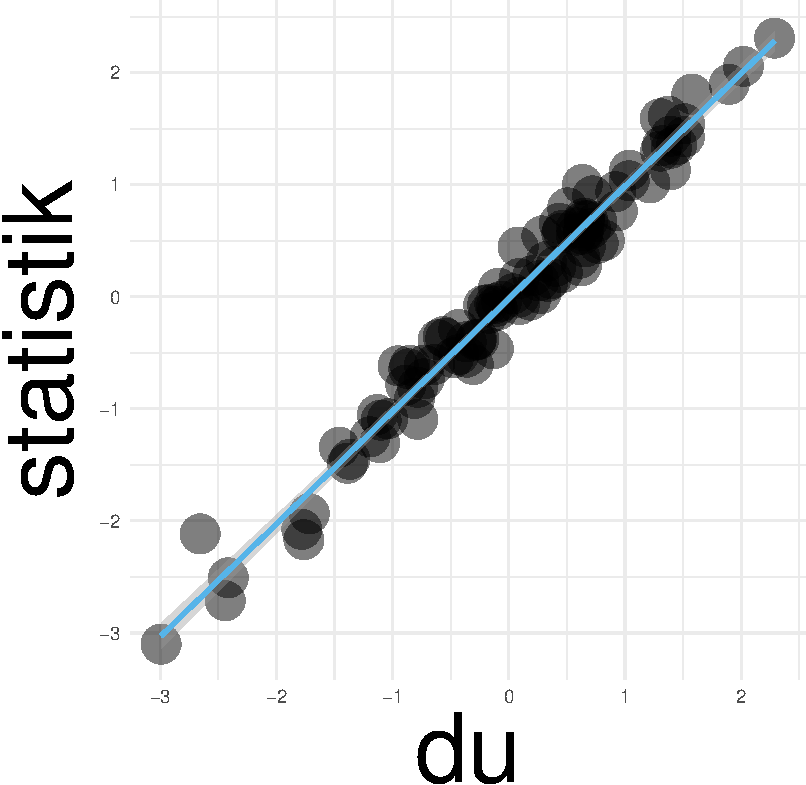
\includegraphics[width=0.33\textwidth,height=\textheight]{005-orga_files/figure-pdf/statistik-und-du-guter-fit-1.pdf}

}

\caption{Statistik und Du: Passt!}

\end{figure}%

\section{Es geht um Ihren Lernerfolg}\label{es-geht-um-ihren-lernerfolg}

Meister Yoda rät: Lesen Sie die folgenden Hinweise, s.
Abbildung~\ref{fig-yoda}.

\begin{figure}

\centering{


\includegraphics[width=0.5\textwidth,height=\textheight]{img/yoda.jpg}

}

\caption{\label{fig-yoda}Lesen Sie die folgenden Hinweise im eigenen
Interesse (imgflip, 2024b)}

\end{figure}%

\href{https://imgflip.com/memegenerator}{Quelle: Imgflip Memengenerator}

\subsection{Lernziele}\label{lernziele}

\begin{itemize}
\item
  Die Studentis sind mit wesentlichen Methoden der explorativen
  Datenanalyse vertraut und können diese selbständig anwenden.
\item
  Die Studentis können gängige Forschungsfragen in lineare Modelle
  übersetzen, diese auf echte Datensätze anwenden und die Ergebnisse
  interpretieren.
\end{itemize}

\subsection{Was lerne ich hier und wozu ist das
gut?}\label{was-lerne-ich-hier-und-wozu-ist-das-gut}

\emph{Was lerne ich hier?}

Sie lernen das \emph{Handwerk der Datenanalyse} mit einem Schwerpunkt
auf Vorhersage. Anders gesagt: Sie lernen, \emph{Daten aufzubereiten}
und aus Daten \emph{Vorhersagen} abzuleiten. Zum Beispiel: Kommt ein
Student zu Ihnen und sagt ``Ich habe 42 Stunden für die Klausur gelernt,
welche Note kann ich in der Klausur erwarten?''. Darauf Ihre Antwort:
``Auf Basis meiner Daten und meines Modells müsstest du eine 2.7
schreiben!''\footnote{Darauf die Studentin: ``Hpmf.''}. Außerdem lernen
Sie, wie man die Güte einer Vorhersage auf Stichhaltigkeit prüft. Denn
Vorhersagen kann man ja in jeder Eckkneipe oder beim Wahrsager bekommen.
Wir wollen aber belastbare Vorhersagen und zumindest wissen, wie gut die
Vorhersagen (von jemanden) bisher waren.

\emph{Warum ist das wichtig?}

Wir wollen nicht auf Leuten vertrauen, die behaupten, sie wüssten, was
für uns richtig und gut ist. Wir wollen selber die Fakten prüfen können.

\emph{Wozu brauche ich das im Job?}

Datenanalyse spielt bereits heute in vielen Berufen eine Rolle. Tendenz
stark zunehmend.

\emph{Wozu brauche ich das im weiterem Studium?}

In Forschungsarbeiten (wie in empirischen Forschungsprojekten, etwa in
der Abschlussarbeit) ist es üblich, statistische Ergebnisse hinsichtlich
quantitativ zu analysieren.

\emph{Ist Statistik nicht sehr abstrakt?}

Der Schwerpunkt dieses Kurses liegt auf Anwenden und Tun; ähnlich dem
Erlernen eines Handwerks. Theorien und Abstraktionen stehen nur am Rand.

\emph{Gibt es auch gute Jobs, wenn man sich mit Daten auskennt?}

Das Forum (2020) berichtet zu den ``Top 20 job roles in increasing and
decreasing demand across industries'' (S. 30, Abb. 22):

\begin{enumerate}
\def\labelenumi{\arabic{enumi}.}
\tightlist
\item
  Data Analysts und Scientists
\item
  AI and Machine Learning Specialists
\item
  Big Data Specialists
\end{enumerate}

\subsection{Was ist hier das
Erfolgsgeheimnis?}\label{was-ist-hier-das-erfolgsgeheimnis}

Das Lesen einer Schwimmfibel ist nur bedingt nützlich, wenn Sie
Freischwimmer werden wollen. Es hilft nichts: Rein in die Fluten! Wenn
das Wasser nicht tief ist, man jederzeit Pause machen kann und die
Erfolge sich schnell einstellen, steht Ihrem Fortschritt beim Lernen
nichts im Weg. Ich gebe zu, der Vergleich ist nicht gerade subtil. Aber
es ist so: Sie lernen durch Tun (Lovett \& Greenhouse, 2000). Dieses
Buch bietet dafür reichhaltige Gelegenheit. Nutzen Sie sie. Jedes
Kapitel führt am Ende eine Reihe von Aufgaben auf, alle mit Lösungen. So
können Sie Ihren Lernfortschritt testen. Das Schwierigkeiten auftreten,
wenn man etwas Neues lernt, ist normal. Das geht fast allen so. Ihren
Lernerfolg kann nur eine Sache gefährden: Wenn Sie aufgaben. Bleiben Sie
dran, und der Erfolg wird sich einstellen! Abbildung~\ref{fig-lernen}
zeigt Daten von N=1646 Studentis, die zeigen, dass regelmäßiges Üben und
Dranbleiben der Schlüssel zum Erfolg ist.

\begin{figure}

\centering{

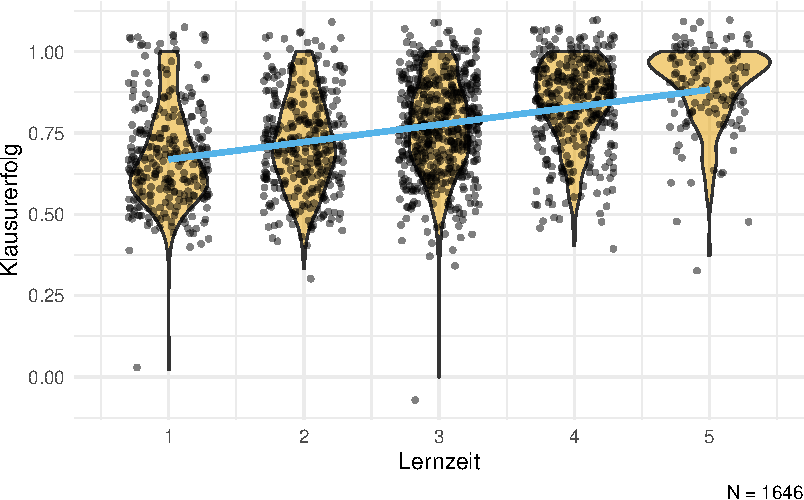
\includegraphics{005-orga_files/figure-pdf/fig-lernen-1.pdf}

}

\caption{\label{fig-lernen}Der Zusammenhang von Lernzeit (1: gering bis
5:hoch) von Klausurerfolg}

\end{figure}%

\begin{tcolorbox}[enhanced jigsaw, titlerule=0mm, left=2mm, toprule=.15mm, opacitybacktitle=0.6, breakable, bottomrule=.15mm, coltitle=black, colframe=quarto-callout-important-color-frame, bottomtitle=1mm, title=\textcolor{quarto-callout-important-color}{\faExclamation}\hspace{0.5em}{Wichtig}, opacityback=0, arc=.35mm, toptitle=1mm, colbacktitle=quarto-callout-important-color!10!white, rightrule=.15mm, leftrule=.75mm, colback=white]

\emph{Dran bleiben} ist der Schlüssel zum Erfolg. Üben Sie regelmäßig.
Geben Sie bei Schwierigkeiten nicht auf.

\emoji{person-lifting-weights} \emoji{clockwise-vertical-arrows}
\emoji{key} \emoji{glowing-star} \(\square\)

\end{tcolorbox}

\subsection{Motivieren Sie mich!}\label{motivieren-sie-mich}

\begin{figure}

\begin{minipage}{0.80\linewidth}
Schauen Sie sich das Video mit einer
\href{https://youtu.be/jtNlzpcPr5Y}{Ansprache zur Motivation}
an.\end{minipage}%
%
\begin{minipage}{0.20\linewidth}

\begin{center}

\includegraphics[width=0.75\textwidth,height=\textheight]{005-orga_files/figure-pdf/unnamed-chunk-2-1.pdf}
\end{center}

\end{minipage}%

\end{figure}%

\subsection{Voraussetzungen}\label{voraussetzungen}

Um von diesem Kurs am besten zu profitieren, sollten Sie Folgendes
mitbringen:

\begin{itemize}
\tightlist
\item
  Bereitschaft, Neues zu lernen
\item
  Bereitschaft, nicht gleich aufzugeben
\item
  Kenntnis grundlegender Methoden wissenschaftlichen Arbeitens
\end{itemize}

Was Sie \emph{nicht} brauchen, sind besondere Mathe- oder
Statistik-Vorkenntnisse.

\subsection{Überblick über das
Buch}\label{uxfcberblick-uxfcber-das-buch}

Abb. Abbildung~\ref{fig-ueberblick} gibt einen Überblick über den
Verlauf und die Inhalte des Buches. Das Diagramm hilft Ihnen zu
verorten, wo welches Thema im Gesamtzusammenhang steht.

\begin{figure}

\centering{

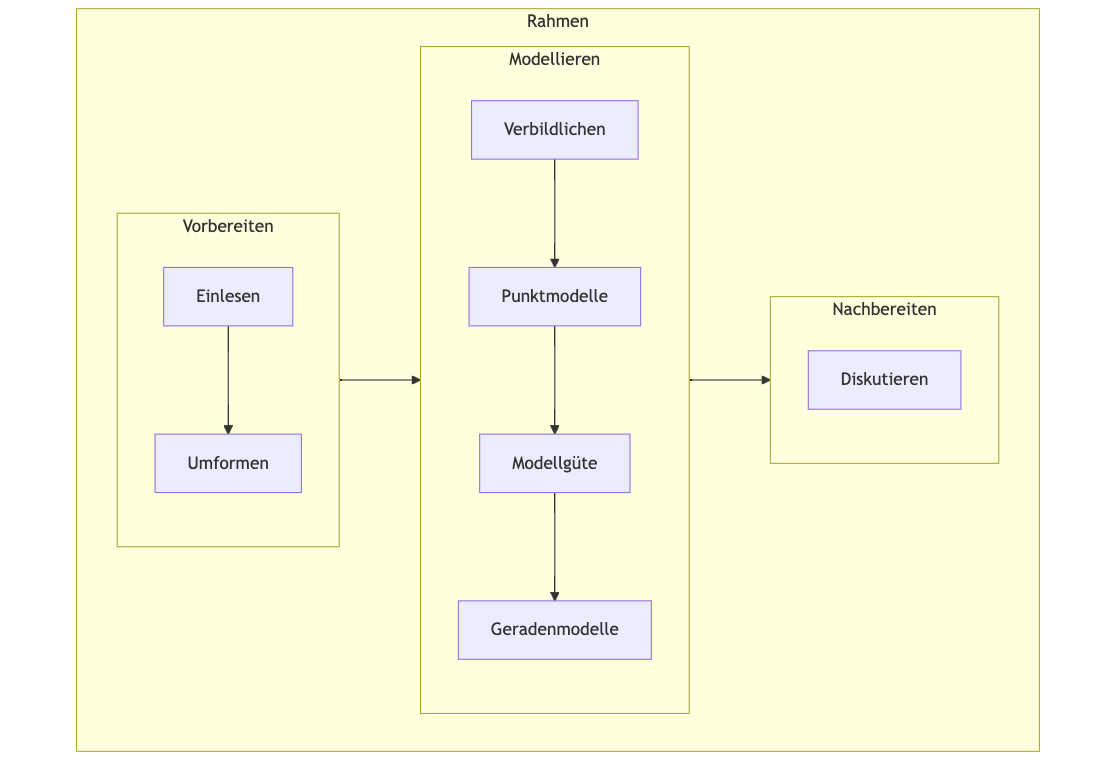
\includegraphics[width=0.7\textwidth,height=\textheight]{img/fig-ueberblick.png}

}

\caption{\label{fig-ueberblick}Überblick über den Inhalt und Verlauf des
Buches}

\end{figure}%

Das Diagramm zeigt auch den Ablauf einer typischen Datenanalyse.
Natürlich kann man sich auch andere sinnvolle Darstellungen dieses
Ablaufs vorstellen.

\section{Lernhilfen}\label{lernhilfen}

\subsection{Aufgaben im Datenwerk}\label{aufgaben-im-datenwerk}

\begin{figure}

\begin{minipage}{0.80\linewidth}
Auf der Webseite \href{https://datenwerk.netlify.app/}{``Datenwerk''}
wird eine große Zahl an Aufgaben bereitgestellt. Am Ende jedes Kapitels
finden Sie eine Auswahl an Aufgabennamen, die Sie im Datenwerk lösen
können.\end{minipage}%
%
\begin{minipage}{0.20\linewidth}

\begin{center}

\includegraphics[width=0.75\textwidth,height=\textheight]{005-orga_files/figure-pdf/unnamed-chunk-3-1.pdf}
\end{center}

\end{minipage}%

\end{figure}%

Außerdem tauchen in jedem Kapitel Übungsaufgaben an verschiedenen
Stellen auf, so dass Sie den jeweiligen Stoff sofort üben und Ihr
Verständnis prüfen können.

\subsection{Videos}\label{videos}

\begin{figure}

\begin{minipage}{0.80\linewidth}
Schauen Sie sich mal den YouTube-Kanal
\texttt{@sebastiansauerstatistics} an und dort die
\href{https://www.youtube.com/playlist?list=PLRR4REmBgpIEaIyeNBgNGPgmhQJ_T1y8_}{Playlist
``R''}. Dort finden Sie einige Videos zum Thema R.\end{minipage}%
%
\begin{minipage}{0.20\linewidth}

\begin{center}

\includegraphics[width=0.75\textwidth,height=\textheight]{005-orga_files/figure-pdf/unnamed-chunk-4-1.pdf}
\end{center}

\end{minipage}%

\end{figure}%

\subsection{Hervorhebungen}\label{hervorhebungen}

Im Buch sind Beispiele, Fehlerquellen, Definitionen und Hinweise visuell
hervorgehoben (und verlinkt), so dass Sie schnell finden können.

\section{Software: R}\label{software-r}

Sie benötigen R, RStudio und einige R-Pakete für diesen Kurs.
\href{https://hinweisbuch.netlify.app/hinweise-software}{Hier} finden
Sie \emph{Installationshinweise.}\footnote{\url{https://hinweisbuch.netlify.app/hinweise-software}}

Dieses Buch enthält ``mittel'' viel R. Auf fortgeschrittene R-Techniken
wurde aber komplett verzichtet. Dem einen Anfänger oder der anderen
Anfängerin mag es dennoch ``viel Code'' erscheinen. Es wäre ja auch
möglich gewesen, auf R zu verzichten und stattdessen eine
``Klick-Software'' zu verwenden. \href{https://jasp-stats.org/}{JASP}
oder \href{https://www.jamovi.org/}{Jamovi} sind Beispiele für tolle
Software aus dieser Kategorie. Ich glaube aber, der Verzicht auf eine
Skriptsprache (R) wäre ein schlechter Dienst an den Studentis. Mit Blick
auf eine ``High-Tech-Zukunft'' sollte man zumindest mit etwas
Computer-Code vertraut sein. Auf Computercode zu verzichten erschiene
mir daher fahrlässig für die ``Zukunftsfestigkeit'' der Ausbildung.

Sie finden den R-Code für jedes Kapitel
\href{https://github.com/sebastiansauer/statistik1/tree/main/R-code-for-all-chapters}{auf
Github}.\footnote{\url{https://github.com/sebastiansauer/statistik1/tree/main/R-code-for-all-chapters}}

\section{Zum Autor}\label{zum-autor}

Nähere Hinweise zum Autor dieses Buch, Sebastian Sauer, finden Sie
\href{https://sebastiansauer-academic.netlify.app/}{hier}.\footnote{\url{https://sebastiansauer-academic.netlify.app/}}
Dort gibt es auch einen Überblick über
\href{https://sebastiansauer-academic.netlify.app/\#ebooks}{weitere
Bücher des Autors zum Themenkreis Datenanalyse}.\footnote{\url{https://sebastiansauer-academic.netlify.app/\#ebooks}}

\section{Griechische Buchstaben}\label{sec-greek}

In diesem Buch werden ein paar (wenige) griechische Buchstaben
verwendet, die in der Statistik üblich sind. Häufig werden
\emph{griechische} Buchstaben verwendet, um eine Grundgesamtheit
(Population) zu beschreiben (die meistens unbekannt ist). Lateinische
(``normale'') Buchstaben werden demgegenüber verwendet, um eine
Stichprobe (Datensatz, vorliegende Daten) zu beschreiben.
Tabelle~\ref{tbl-griech} stellt diese Buchstaben zusammen mit ihrer
Aussprache und Bedeutung vor.

\begin{longtable}[]{@{}lllr@{}}
\caption{Griechische Buchstaben, die in diesem Buch verwendet
werden.}\label{tbl-griech}\tabularnewline
\toprule\noalign{}
Zeichen & Aussprache & Buchstabe & Bedeutung in der Statistik \\
\midrule\noalign{}
\endfirsthead
\toprule\noalign{}
Zeichen & Aussprache & Buchstabe & Bedeutung in der Statistik \\
\midrule\noalign{}
\endhead
\bottomrule\noalign{}
\endlastfoot
\(\beta\) & beta & b & Regressionskoeffizent \\
\(\mu\) & mü & m & Mittelwert \\
\(\sigma\) & sigma & s & Streuung \\
\(\Sigma\) & Sigma & S & Summenzeichen \\
\(\rho\) & rho & r & Korrelation (nach Pearson) \\
\end{longtable}

Mehr griechische Buchstaben finden sich
\href{https://de.wikipedia.org/wiki/Griechisches_Alphabet}{z.B. in
Wikipedia}.\footnote{\url{https://de.wikipedia.org/wiki/Griechisches_Alphabet}}

\section{Reproduzierbarkeit}\label{reproduzierbarkeit}

Die verwendeten R-Pakete sind mit
\href{https://rstudio.github.io/renv/index.html}{renv}
dokumentiert.\footnote{\url{https://rstudio.github.io/renv/index.html}}
Der Quellcode ist \href{https://github.com/sebastiansauer/statistik1}{in
diesem Github-Repo} dokumentiert.\footnote{\url{https://github.com/sebastiansauer/statistik1}}

\part{Vorbereiten}

\chapter{Rahmen}\label{rahmen}

\[
\definecolor{ycol}{RGB}{230,159,0}
\definecolor{modelcol}{RGB}{86,180,233}
\definecolor{errorcol}{RGB}{0,158,115}
\definecolor{beta0col}{RGB}{213,94,0}
\definecolor{beta1col}{RGB}{0,114,178}
\definecolor{xcol}{RGB}{204,121,167}
\]

\section{Lernsteuerung}\label{lernsteuerung}

Abbildung~\ref{fig-ueberblick} zeigt den Standort dieses Kapitels im
Lernpfad und gibt damit einen Überblick über das Thema dieses Kapitels
im Kontext aller Kapitel. Abbildung~\ref{fig-tidy5} zeigt, dass unser
Vorgehen in diesem Buch einem Fließband gleicht: Schritt für Schritt, in
der richtigen Reihenfolge, vom Anfang bis Ende, erarbeiten wir unser
``Datenprodukt''.

\begin{figure}

\centering{

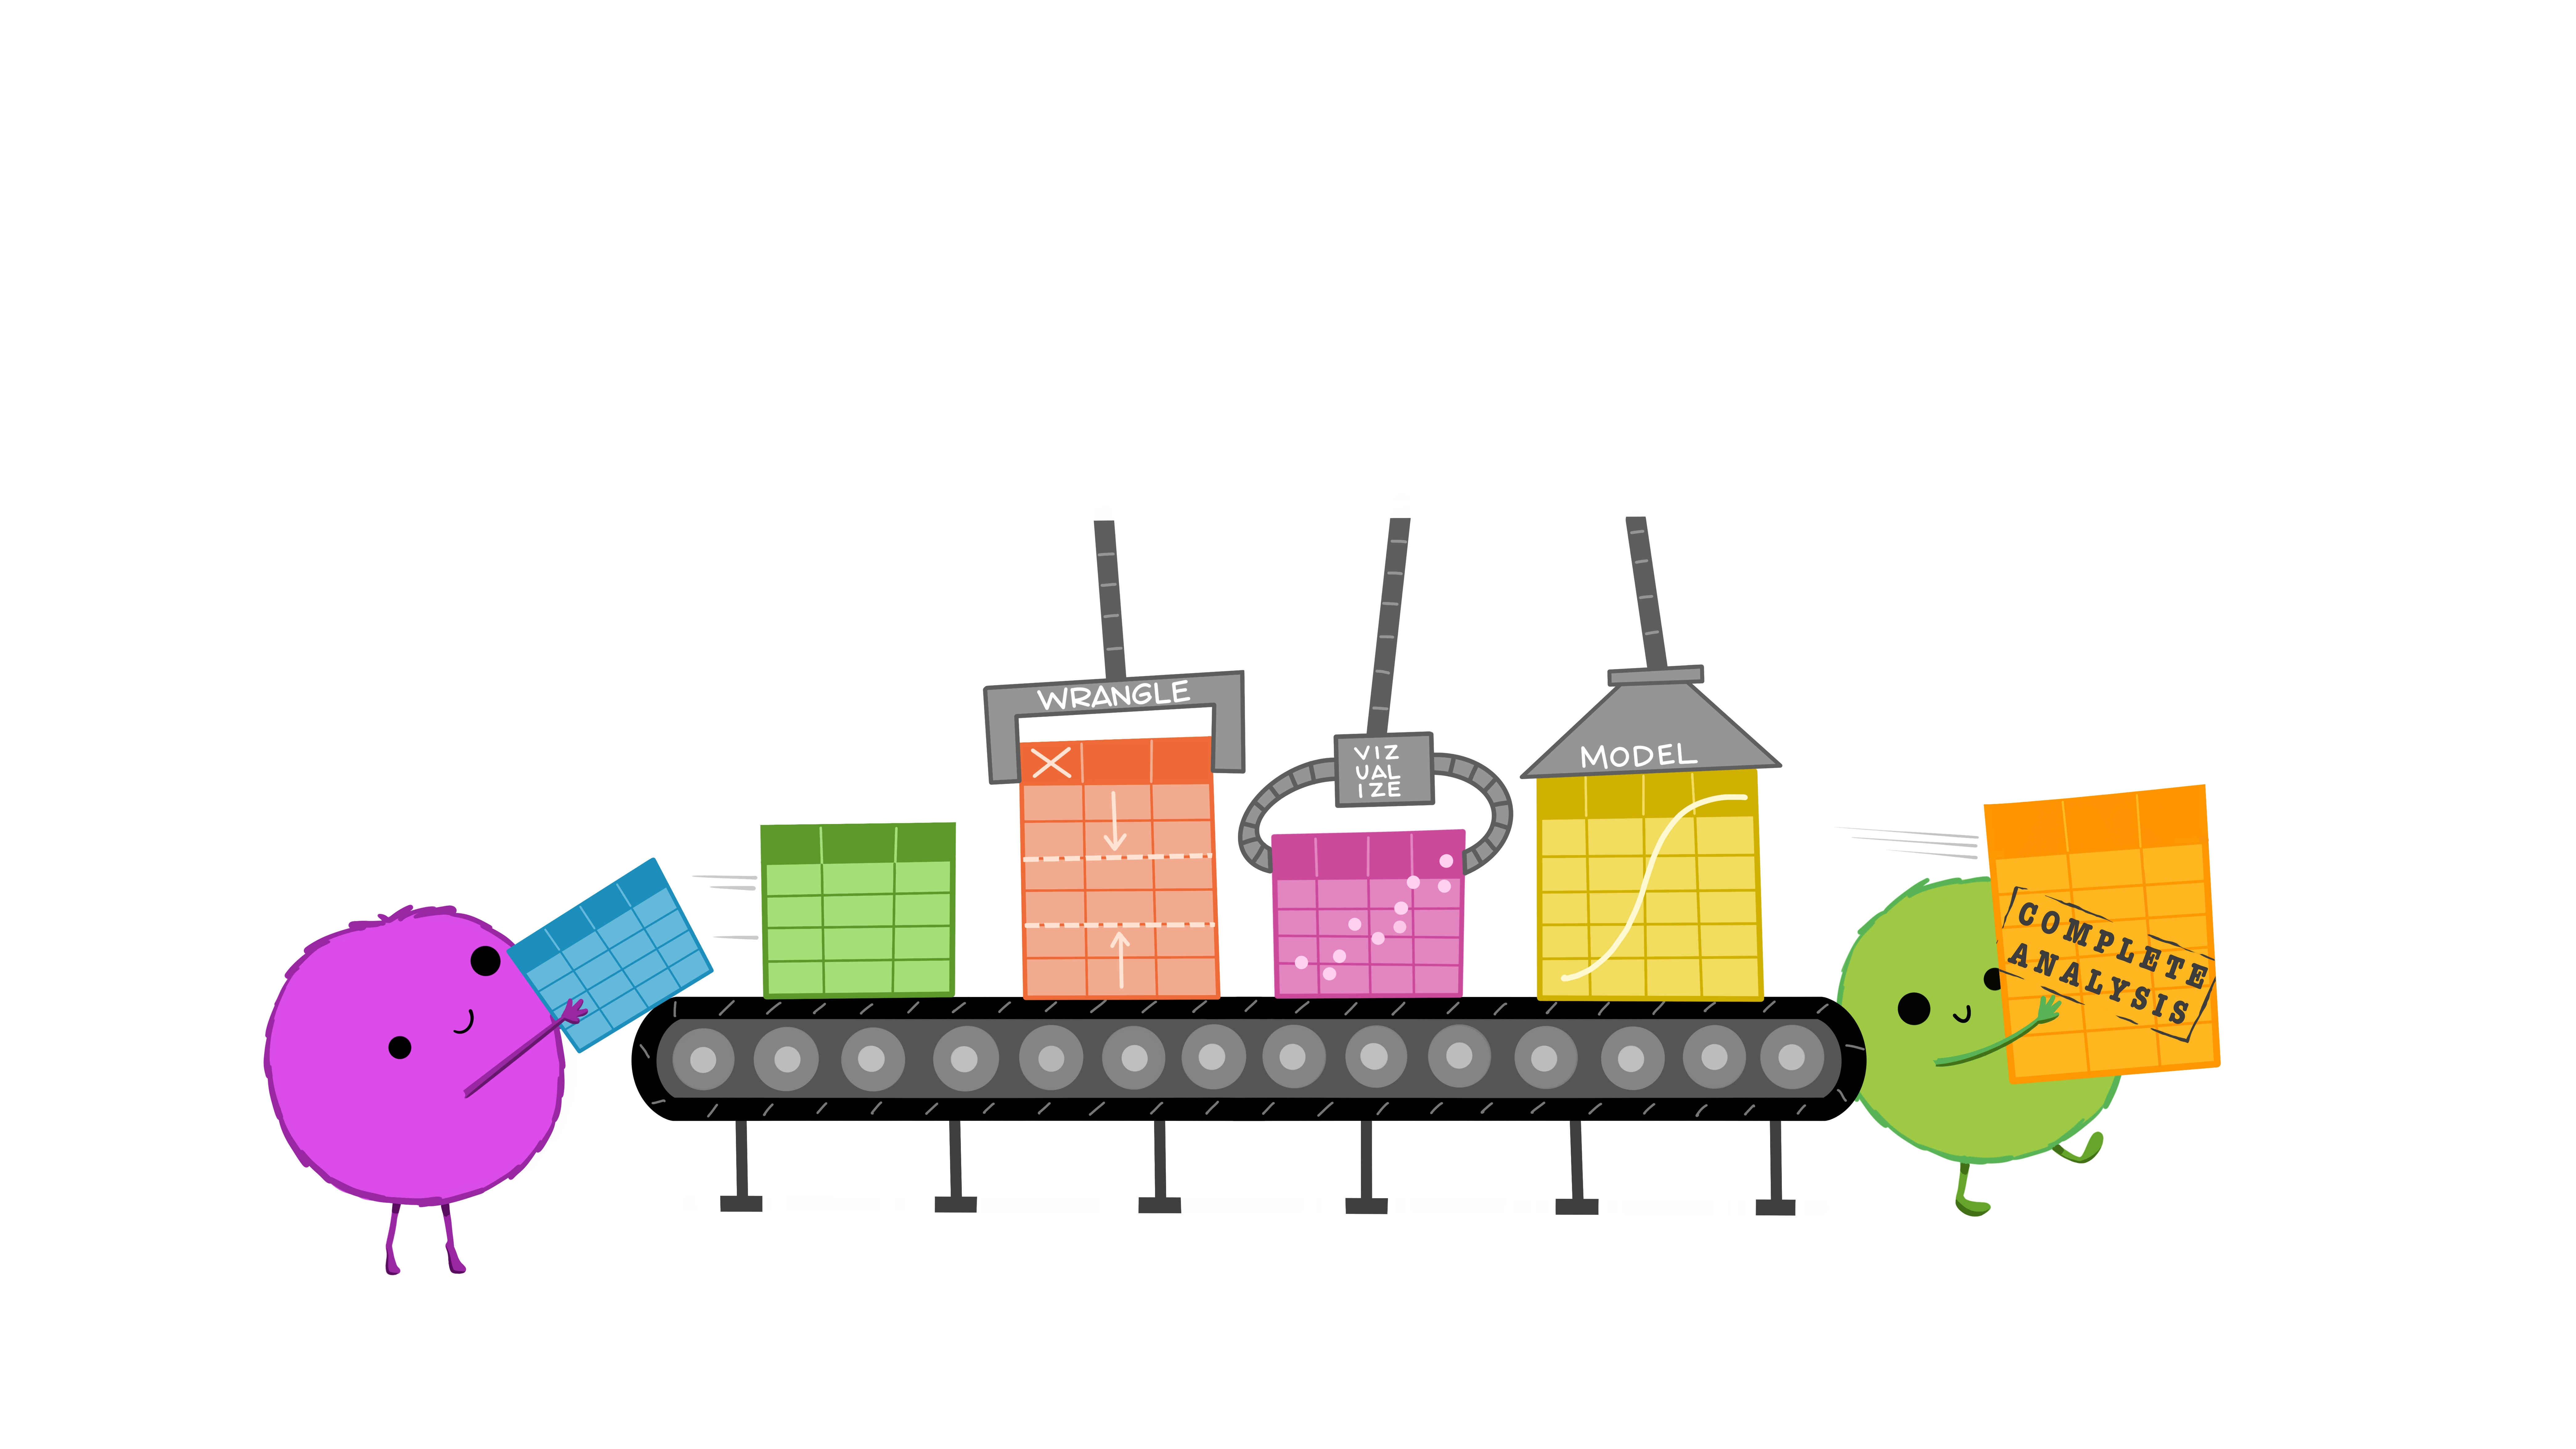
\includegraphics[width=0.75\textwidth,height=\textheight]{img/tidydata_5.jpg}

}

\caption{\label{fig-tidy5}Datenanalyse als eine Abfolge am Fließband
(Horst, 2024)}

\end{figure}%

\subsection{Lernziele}\label{lernziele-1}

\begin{itemize}
\tightlist
\item
  Sie können eine Definition von Statistik wiedergeben.
\item
  Sie können eine Definition von Daten wiedergeben.
\item
  Sie können den Begriff Tidy-Daten erläutern.
\item
  Sie können Beispiele für verschiedene Skalenniveaus nennen.
\end{itemize}

\subsection{Erfolsgrezept}\label{erfolsgrezept}

Ihren Lernerfolg kann man als von drei Faktoren abhängig betrachten: 1)
Ihrer Lehrkraft, 2) Ihrer Mitarbeit im Unterricht und 3) Ihrem
Eigenstudium zuhause (Vor- bzw. Nachbereitung des Unterrichts), s.
Abbildung~\ref{fig-erfolgsrezept}.

\begin{figure}

\centering{

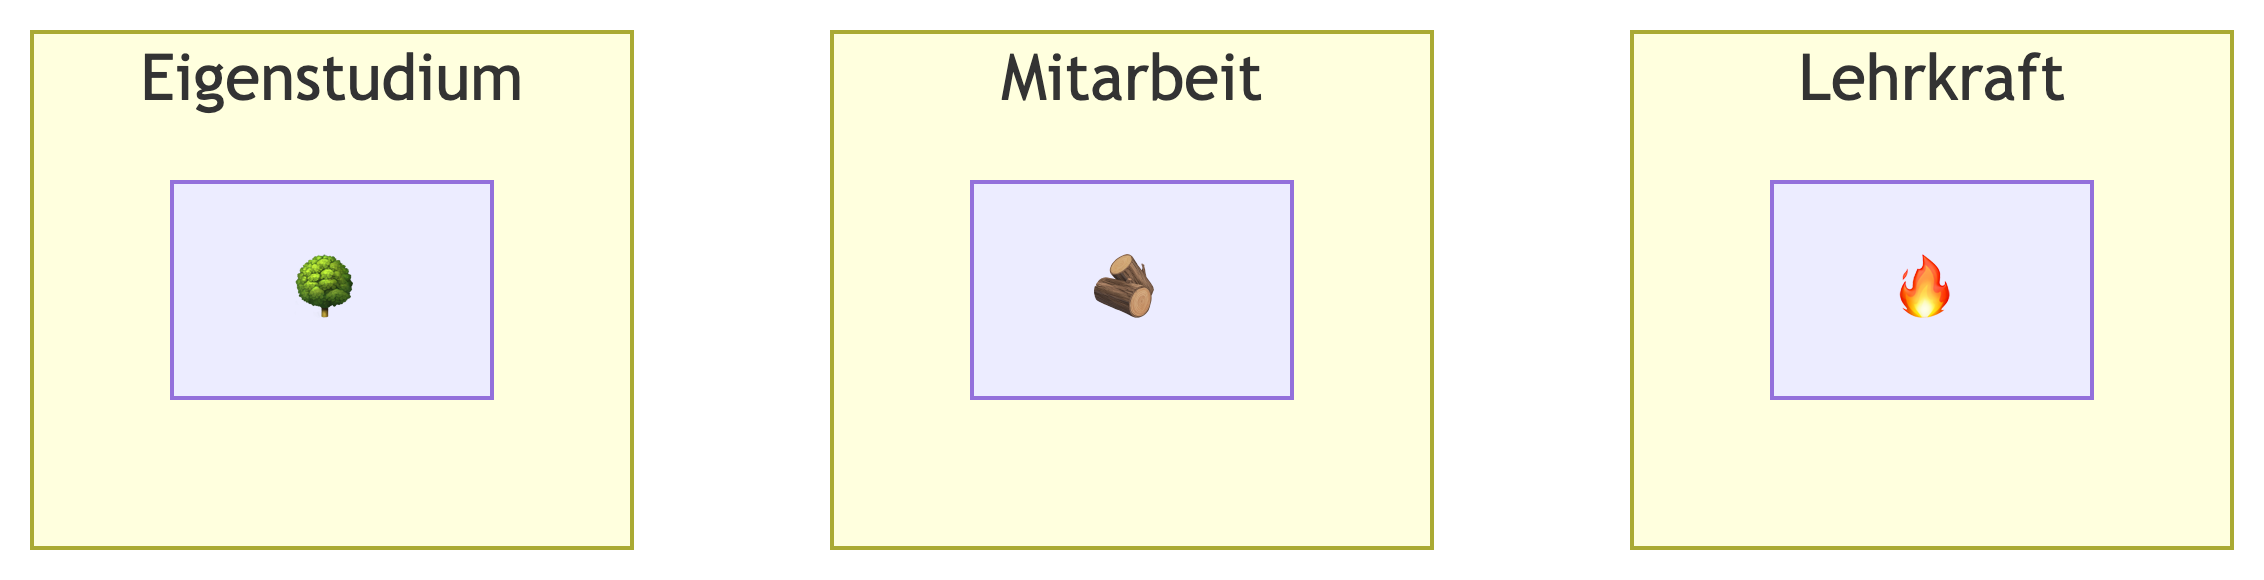
\includegraphics[width=5.42in,height=1.06in]{010-rahmen_files/figure-latex/mermaid-figure-1.png}

}

\caption{\label{fig-erfolgsrezept}Ihr Lernerfolg besteht aus drei
Komponenten: Der Lehrkraft, Ihrer Konzentration im Unterricht und Ihrer
Vor- bzw. Nachbereitung zuhause.}

\end{figure}%

Eine gute Lehrkraft ist wie der Funke, der eine (Lern-)Flamme entzündet.
Aber es braucht Brennmaterial, einen Holzscheit, das ist Ihre
Konzentration im Unterricht. Ein Holzscheit alleine ist aber nicht
nachhaltig, es braucht viel mehr Brennmaterial, um das Feuer am Leben zu
halten: Ihr Eigenstudium, das stetige, selbständige Beschäftigen mit der
Materie.

\section{Was ist Statistik und wozu ist sie
gut?}\label{was-ist-statistik-und-wozu-ist-sie-gut}

In diesem Buch werden die Begriffe \emph{Statistik}, \emph{Datenanalyse}
und \emph{Data Science} synonym verwendet.

\begin{exercise}[Nutzen von
Statistik]\protect\hypertarget{exr-nutzen-statistik}{}\label{exr-nutzen-statistik}

Fragen Sie einen Chatbot (wie ChatGPT), was der Nutzen von Statistik
ist. Diskutieren Sie die Antwort. \(\square\)

\end{exercise}

Hm. Vielleicht fragen wir mal ChatGPT, was es unter Statistik versteht:

\begin{quote}
{\emoji{student}} Was ist Statistik? Bitte definiere verständlich.
\end{quote}

\begin{quote}
{\emoji{robot}} Statistik ist eine Wissenschaft, die sich mit der
Sammlung, Analyse, Interpretation, Präsentation und Übertragung von
Daten beschäftigt. Ziel ist es, Muster und Trends in den Daten zu
erkennen und verlässliche Schlussfolgerungen über eine größere Gruppe
(z.B. Bevölkerung) auf der Basis einer Stichprobe (Teilmenge) zu
treffen. Die Statistik hilft uns bei der Beantwortung von Fragen, indem
sie uns dabei hilft, die Unsicherheit in den Daten zu messen und zu
verstehen\footnote{Release 2023-Jan}.
\end{quote}

Es gibt mehrere Definition von Statistik; hier ist eine, s.
Definition~\ref{def-statistik}.

\begin{definition}[Statistik]\protect\hypertarget{def-statistik}{}\label{def-statistik}

Statistik fasst Daten zusammen, um wesentliche Informationen den Daten
zu entnehmen und beschreibt die Ungewissheit unserer Schlüsse (Kaplan,
2009; Poldrack, 2023) .\(\square\)

\end{definition}

Betrachten wir die zwei Bestimmungsstücke einer Definition von Statistik
genauer:

\begin{enumerate}
\def\labelenumi{\arabic{enumi}.}
\tightlist
\item
  Daten zusammenfassen
\item
  Ungewissheit beschreiben
\end{enumerate}

\subsection{Daten zusammenfassen}\label{daten-zusammenfassen}

Abbildung~\ref{fig-zsmnfassen} verdeutlicht das Prinzip des
Zusammenfassens von Daten. Anschaulich gesprochen: Eine Menge von Zahlen
wird zu einer einzelnen Zahl ``zusammengedampft''. Eine einzelne Zahl
ist wesentlich besser zu verstehen als eine große Menge von Zahlen. Bei
vielen Zahlen würde man den Überblick verlieren.

\begin{figure}

\begin{minipage}{0.45\linewidth}

\centering{

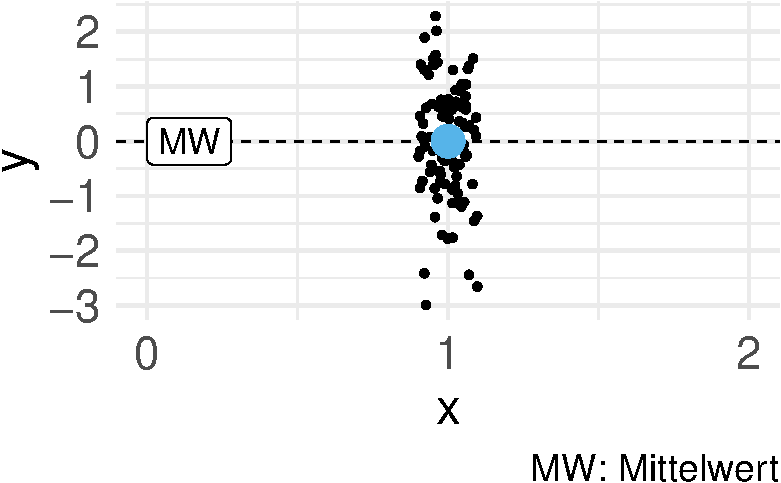
\includegraphics{010-rahmen_files/figure-pdf/fig-zsmnfassen-1.pdf}

}

\subcaption{\label{fig-zsmnfassen-1}Zusammenfassen einer Variable zu
einem Punktwert, hier zum Mittelwert}

\end{minipage}%
%
\begin{minipage}{0.10\linewidth}
~\end{minipage}%
%
\begin{minipage}{0.45\linewidth}

\centering{

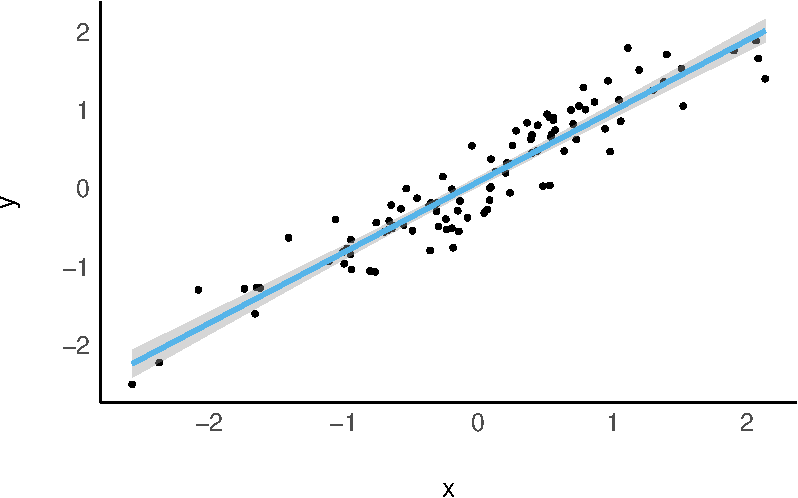
\includegraphics{010-rahmen_files/figure-pdf/fig-zsmnfassen-2.pdf}

}

\subcaption{\label{fig-zsmnfassen-2}Zusammenfassen zweier Variablen zu
einer Geraden}

\end{minipage}%

\caption{\label{fig-zsmnfassen}Daten zusammenfassen}

\end{figure}%

\subsection{Unterschiedlichkeit
messen}\label{unterschiedlichkeit-messen}

Eine allgegenwärtige Tatsache ist, dass die Dinge der Welt sich
unterscheiden, etwa, dass Exemplare einer Gattung sich unterscheiden. So
sind nicht alle Menschen gleich groß, nicht alle Bücher gleich lang oder
nicht alle Tage gleich warm.

Ein zentrales Vorgehen bei statistischen Analysen ist es, die
\emph{Unterschiedlichkeit der Dinge} zu beschreiben, präziser gesagt:
die \emph{Variation zu quantifizieren}. Betrachten wir dazu das Beispiel
in s. Abbildung~\ref{fig-groesse}.

\begin{figure}

\centering{

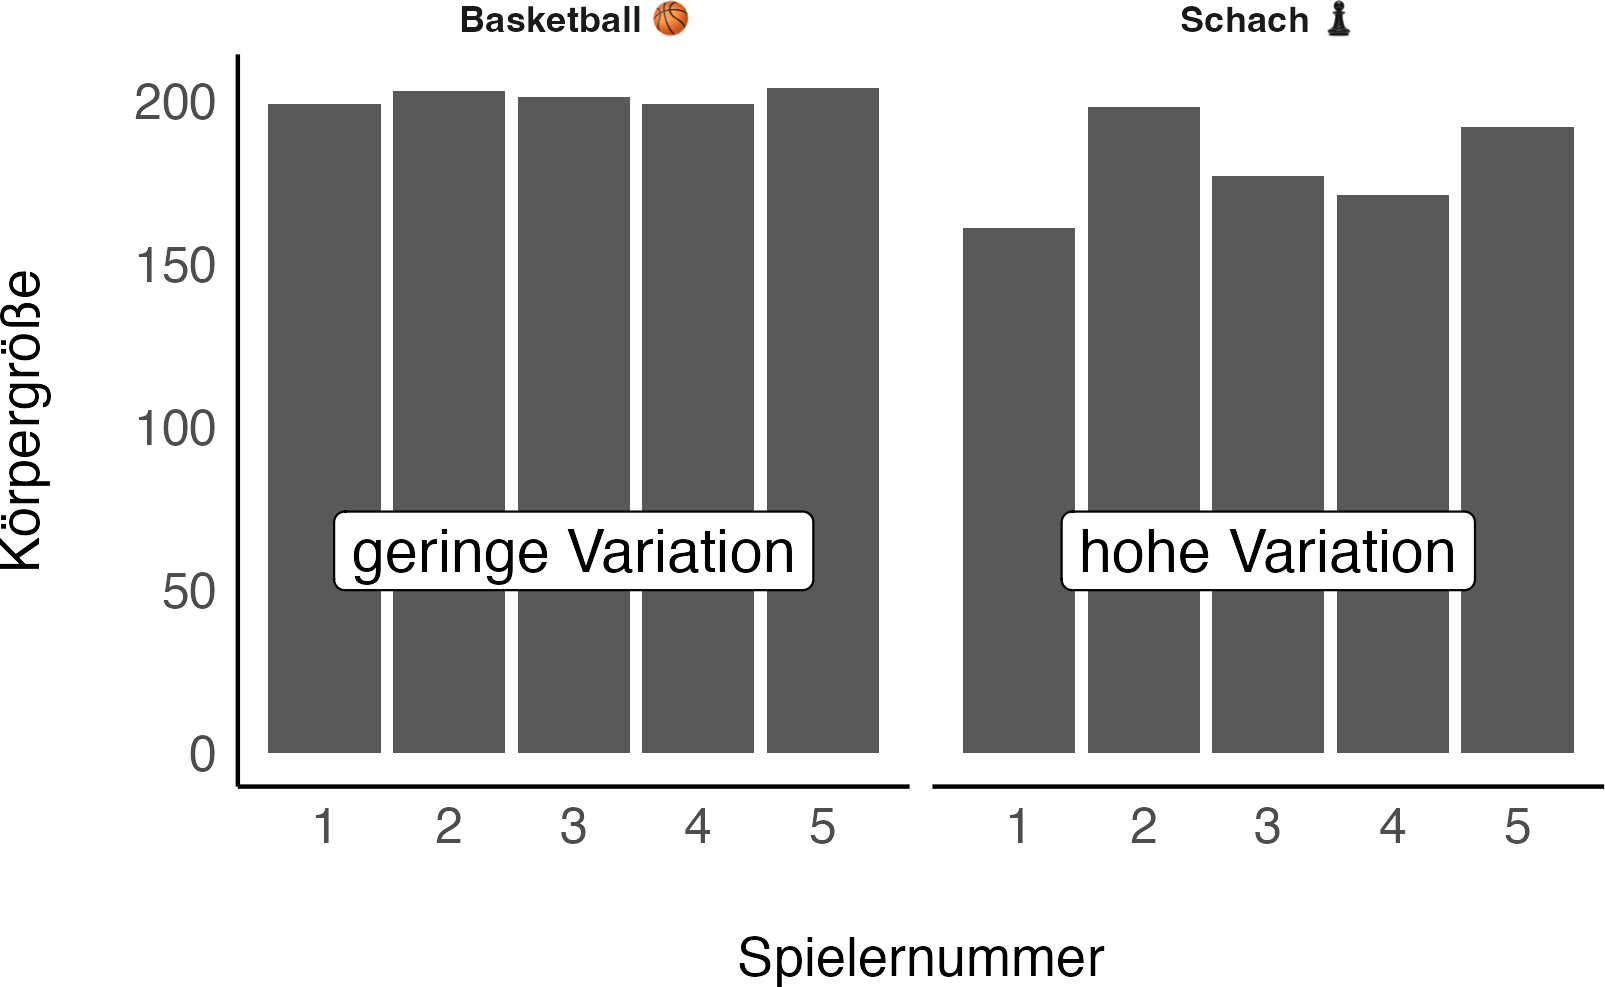
\includegraphics{010-rahmen_files/figure-pdf/fig-groesse-1.png}

}

\caption{\label{fig-groesse}Wenig Variation in der Körpergröße bei den
Basketballern. Alles lange Kerle. Viel Variation bei den Schachspielern:
Manche sind klein, ander groß.}

\end{figure}%

Bei den Basketballern gibt es \emph{geringe} Variation in der
Körpergröße - alle sind groß, ähnlich groß. Bei den Schachspielern gibt
es (im Verhältnis) \emph{hohe} Variation: Einige Personen sind groß,
andere klein.

Die Variation (auch ``Variabilität'' genannt) kann man auch gut so
darstellen wie in s. Abbildung~\ref{fig-variab} gezeigt.

\begin{figure}

\centering{

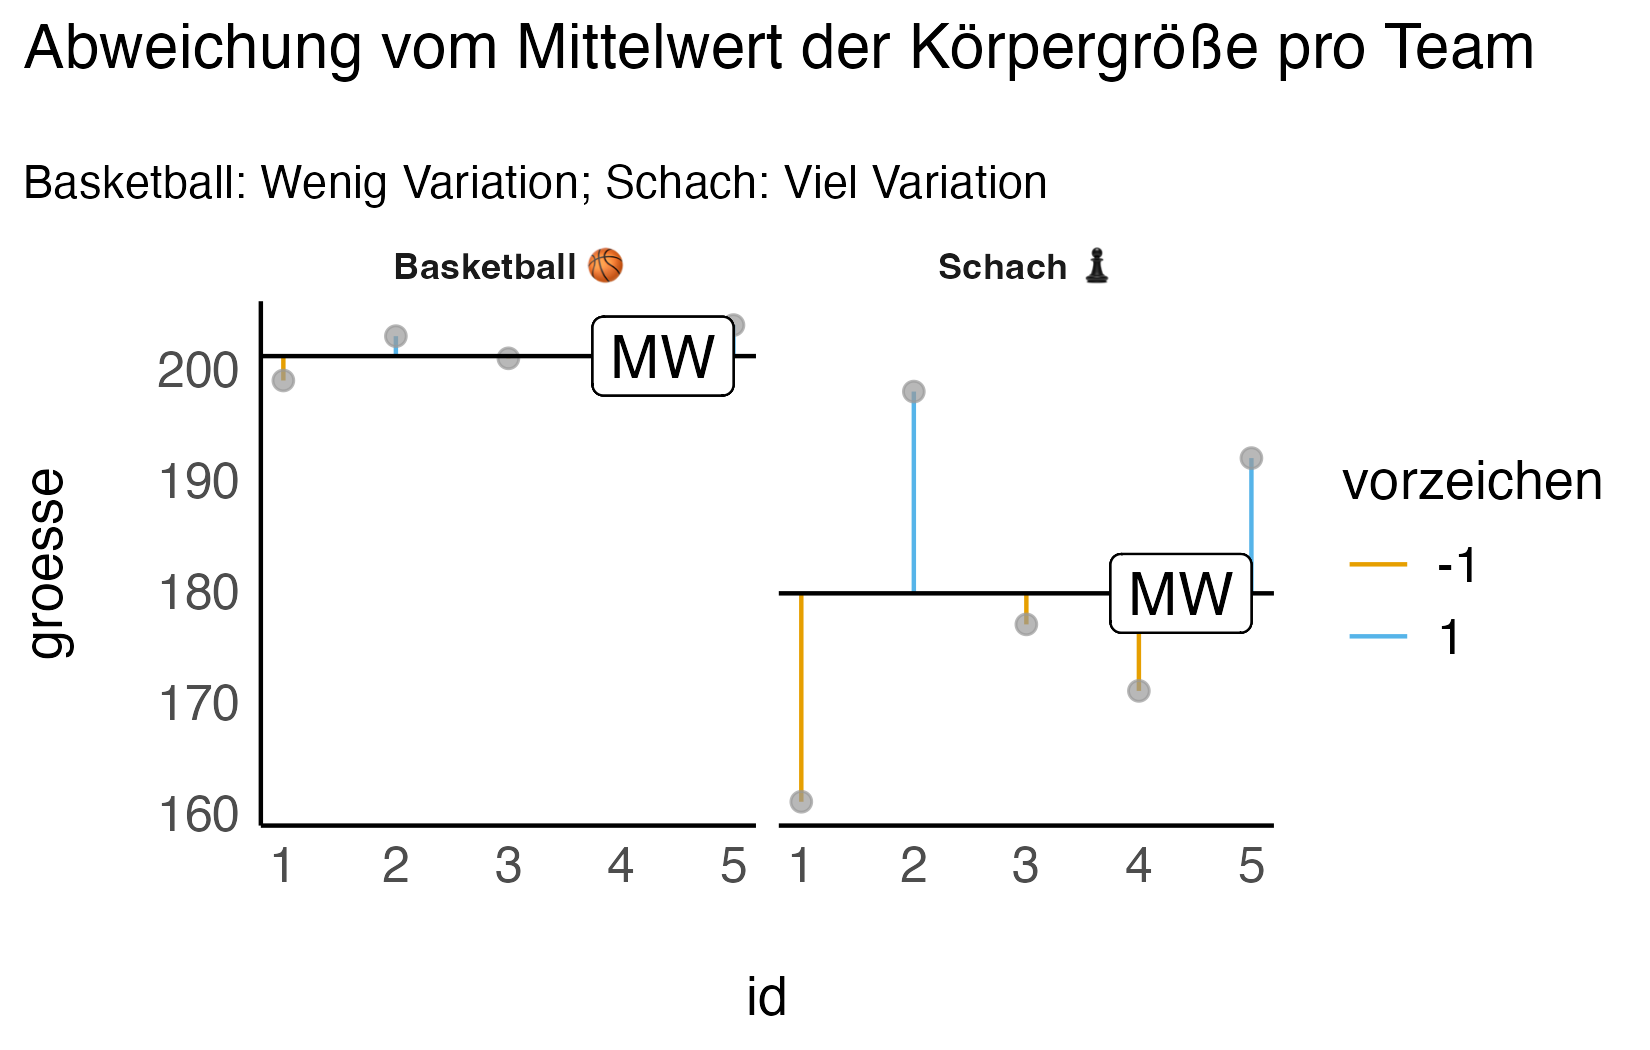
\includegraphics{010-rahmen_files/figure-pdf/fig-variab-1.png}

}

\caption{\label{fig-variab}Die Abweichungen der einzelnen Personen von
der mittleren Körpergröße ihres Teams}

\end{figure}%

Eine \emph{Abweichung} (auch \emph{Residuum}) genannt, zeigt hier die
Differenz von Mittelwert und dem Wert der Körpergröße bei der jeweiligen
Person. Wenn wir allgemein von einer Person \(i\) sprechen, Das Merkmal
\emph{Körpergröße} mit \(X\) bezeichnen und den Mittelwert der
Körpergröße als \(\bar{x}\) (``x quer''), dann können wir knapp und
präzise das Residuum der \(i\)-ten Person mit \(r_i\) bezeichnen und
entsprechend definieren.

\begin{definition}[Residuum]\protect\hypertarget{def-residuum}{}\label{def-residuum}

Das Residuum des Merkmals \(X\) der \(i\)-ten Beobachtung ist definiert
als die Differenz vom Wert \(x_i\) und einem Referenzwert, etwa dem
Mittelwert, \(\bar{x}\):

\(r_i = x_i - \bar{x}\). \(\square\)

\end{definition}

\section{Was ist das Ziel Ihrer
Analyse?}\label{was-ist-das-ziel-ihrer-analyse}

\subsection{Arten von Zielen}\label{arten-von-zielen}

\begin{figure}

\centering{

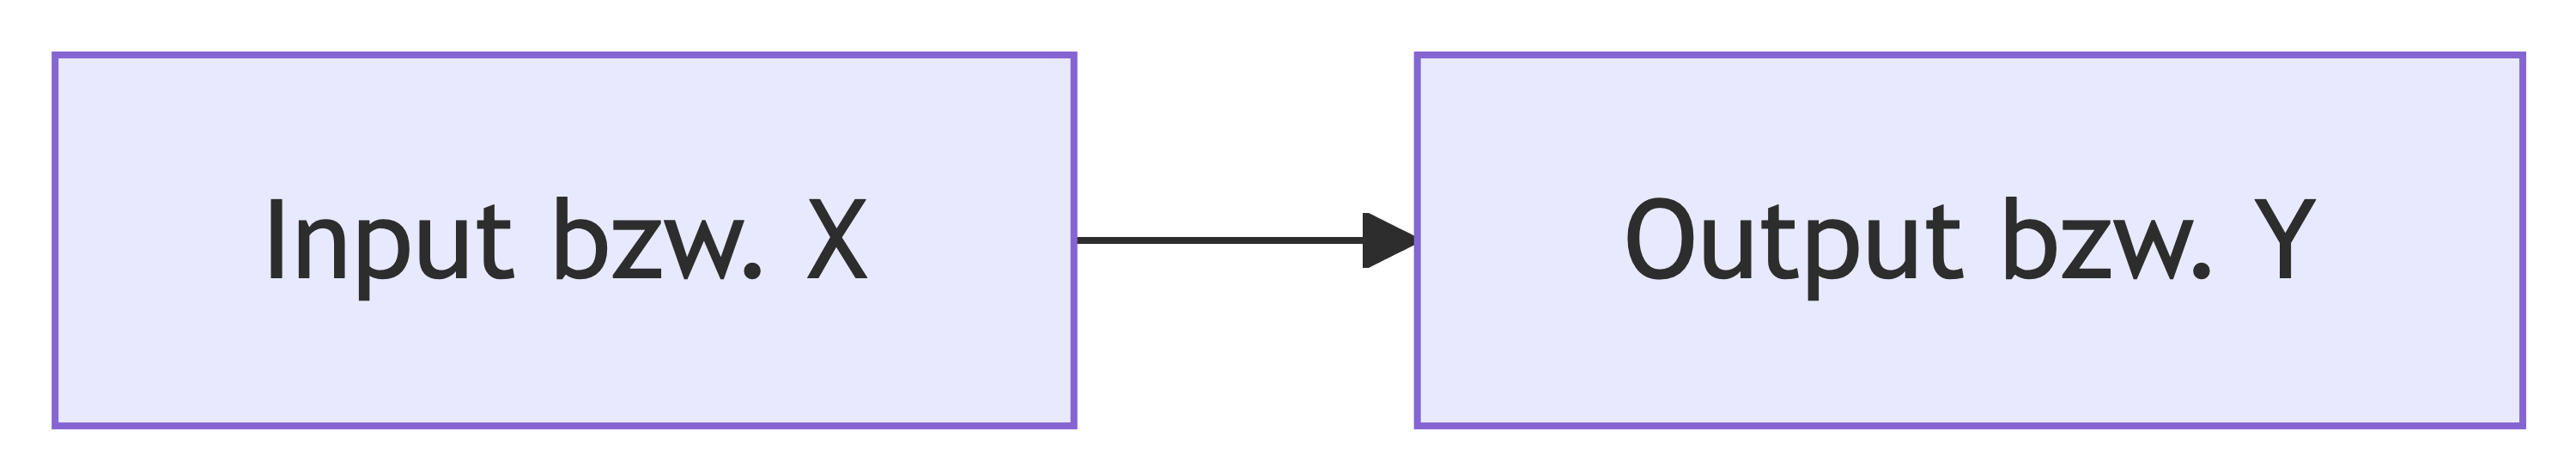
\includegraphics[width=4.84in,height=1.04in]{010-rahmen_files/figure-latex/mermaid-figure-6.png}

}

\caption{\label{fig-ziele}Zielarten einer Datenanalyse}

\end{figure}%

Beispiele für die einzelnen Zielarten der Datenanalyse:

\begin{itemize}
\tightlist
\item
  \emph{Beschreiben}: Wie groß ist der Gender-Paygap in der Branche X im
  Zeitraum Y?
\item
  \emph{Vorhersagen}: Wenn ich 100 Stunden auf die Statistikklausur
  lernen, welche Note kann ich dann erwarten?
\item
  \emph{Erklären}: Wie viel bringt mir das Lernen auf die
  Statistikklausur?
\end{itemize}

\begin{exercise}[]\protect\hypertarget{exr-ziele-stat}{}\label{exr-ziele-stat}

Benennen Sie Beispiele für die die drei Zielarten von Datenanalysen!
\(\square\)

\end{exercise}

\subsection{Forschungsfrage}\label{forschungsfrage}

Eine Forschungsfrage ist die Leitfrage Ihrer Analyse. Sie definiert, was
Sie herausfinden wollen. Häufig sind Forschungsfragen so aufgebaut:

\begin{quote}
Hat X einen Einfluss auf Y?
\end{quote}

Eine Forschungsfrage weist häufig folgende Struktur auf, s.
Abbildung~\ref{fig-fo-struktur}.

\begin{figure}

\centering{

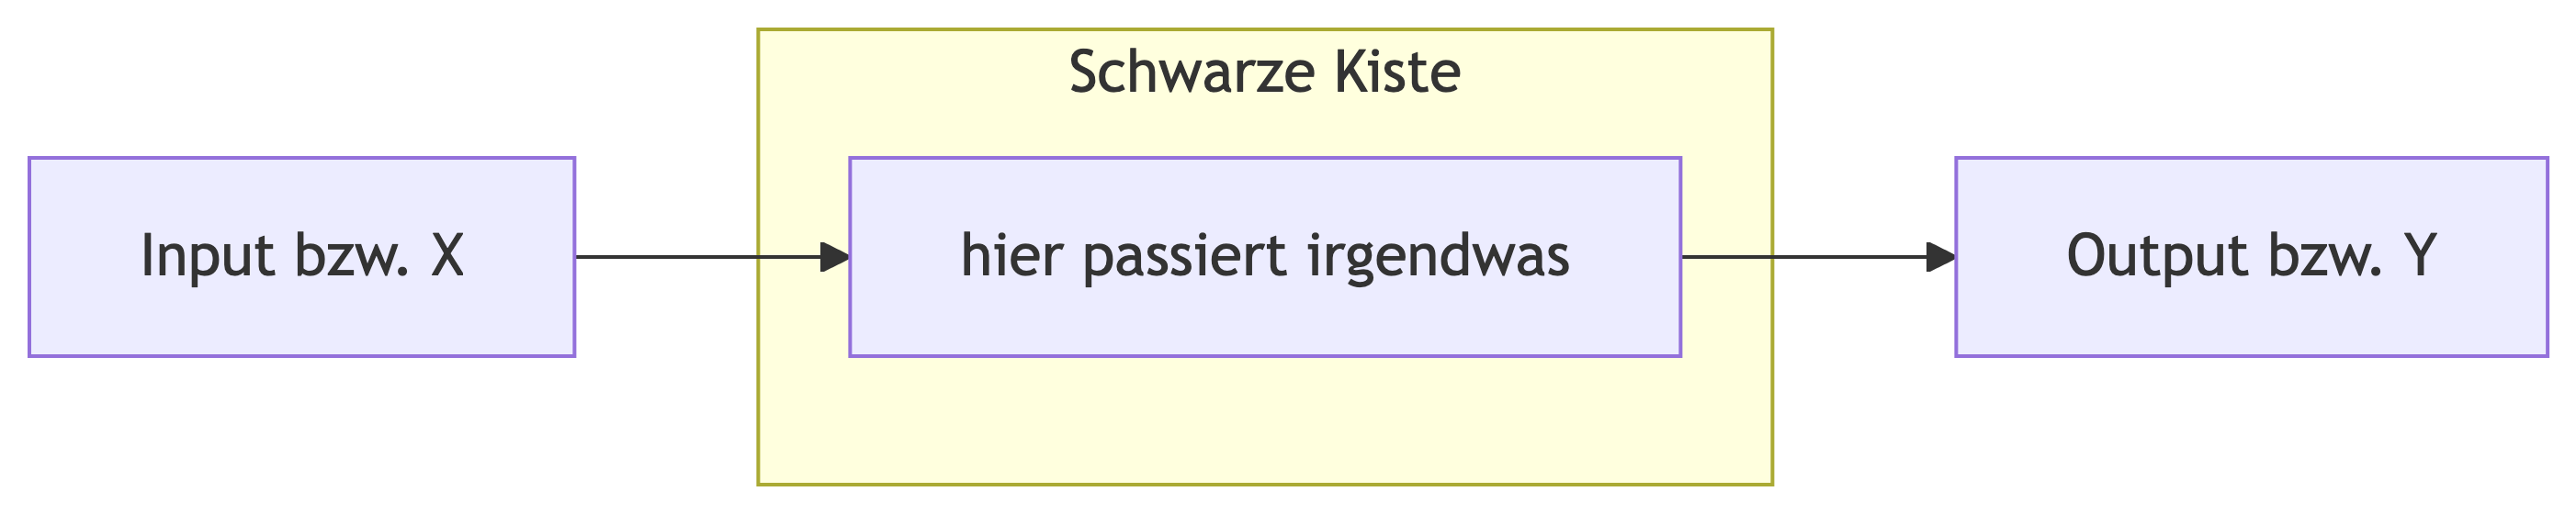
\includegraphics[width=5.9in,height=1.24in]{010-rahmen_files/figure-latex/mermaid-figure-5.png}

}

\caption{\label{fig-fo-struktur}Struktur eine Forschungsfrage}

\end{figure}%

\begin{example}[Forschungsfrage
1]\protect\hypertarget{exm-fofrage1}{}\label{exm-fofrage1}

~

\begin{quote}
Hat Lernen (X) einen Einfluss auf den Prüfungserfolg (Y)? Verringert
Joggen (X) die Menge des Hüftgolds (Y)? Um welchen Betrag erhöht sich
der Umsatz (Y), wenn wir 1000€ mehr Werbung ausgeben? (X)\(\square\)
\end{quote}

\end{example}

\begin{example}[Forschungsfrage
2]\protect\hypertarget{exm-fofrage2}{}\label{exm-fofrage2}

Nach dem Studium haben Sie bei einem großen Online-Auktionshaus
angeheuert. Da Sie angaben, sich im Studium \st{intensiv} etwas mit
Statistik beschäftigt zu haben, hat man Sie in die Abteilung für
Forschung und Entwicklung (F\&E) gesteckt. Heute ist es Ihre Aufgabe,
Auktionen zur Spielekonsole
\href{https://www.nintendo.de/Wii/Wii-94559.html}{Wii} zu
untersuchen,\footnote{\url{https://www.nintendo.de/Wii/Wii-94559.html}}
genauer gesagt geht es um das Spiel
\href{https://www.nintendo.de/Spiele/Wii/Mario-Kart-Wii-281848.html\#_bersicht}{Mariokart}.\footnote{y\url{https://www.nintendo.de/Spiele/Wii/Mario-Kart-Wii-281848.html\#_bersicht}}
Ihre Forschungsfrage lautet:

\begin{quote}
Welche Produktmerkmale stehen mit einem hohen Verkaufserlös in
Zusammenhang?\(\square\)
\end{quote}

\end{example}

\begin{example}[Handynutzung und
Konzentrationsfähigkeit]\protect\hypertarget{exm-braindrain}{}\label{exm-braindrain}

Eine Forschungsfrage könnte lauten zum Thema Handynutzung:

\begin{quote}
Verringert intensive Handynutzung die Konzentrationsfähigkeit?
\(\square\)
\end{quote}

\end{example}

\begin{example}[]\protect\hypertarget{exm-braindrain2}{}\label{exm-braindrain2}

~

\subsection{Aus der Forschung:
Smartphone-Brain-Drain}\label{aus-der-forschung-smartphone-brain-drain-1}

Ward et al. (2017) untersuchten die Forschungsfrage, ob die bloße
Gegenwart eines Handies (z.B. wenn es vor Ihnen auf dem Tisch liegt)
dazu führt, dass man abgelenkt wird und daher schlechtere kognitive
Leistungen zeigt.

Leider schreiben die Autoren Ihre Hypothese nicht glasklar, aber
implizit ist obige Hypothese herauszulesen:

\begin{quote}
First, smartphones may redirect the orientation of conscious attention
away from the focal task and toward thoughts or behaviors associated
with one's phone. Prior research provides ample evidence that \ldots{}
this digital distraction adversely affects both performance \ldots{} and
enjoyment.
\end{quote}

Später formulieren Sie Ihre Hypothese noch genauer:

\begin{quote}
In two experiments, we test the hypothesis that the mere presence of
one's own smartphone reduces available cognitive capacity.
\end{quote}

Die Ergebnisse unterstützen Ihre Hypothese, s.
Abbildung~\ref{fig-braindrain}. Im Diagramm ist ersichtlich, dass die
kognitive Leistung (Y-Achse) sowohl in der Kapazität des
Arbeitsgedächtnisses (links) als auch in der fluiden Intelligenz
(rechts) am geringsten ist, wenn das Handy auf dem Schreibtisch (Desk)
liegt. Am besten ist die kognitive Leistung, wenn das Handy nicht im
Raum ist.\(\square\)

\begin{figure}

\centering{

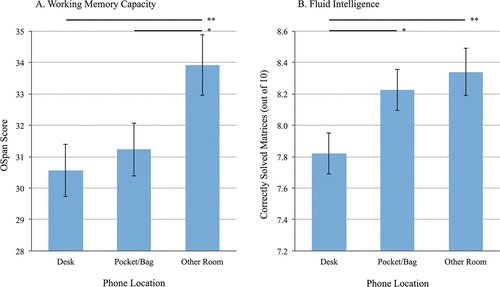
\includegraphics{img/braindrain1.jpg}

}

\caption{\label{fig-braindrain}Handy in Sichtweite verringert die
kognitiven Ressourcen, Ward et al. (2017)}

\end{figure}%

\end{example}

\begin{exercise}[]\protect\hypertarget{exr-braindrain1}{}\label{exr-braindrain1}

Benennen Sie X und Y in Beispiel~\ref{exm-braindrain2}! \(\square\)

\end{exercise}

\begin{exercise}[]\protect\hypertarget{exr-braindrain-chatgpt}{}\label{exr-braindrain-chatgpt}

Fragen Sie einen Bot (z.B. ChatGPT) zum Stand der Forschung hinsichtlich
der Braindrain-Forschungsfrage. Diskutieren Sie die Antwort, auch in
ihren Grenzen. \(\square\)

\end{exercise}

\begin{tcolorbox}[enhanced jigsaw, titlerule=0mm, left=2mm, toprule=.15mm, opacitybacktitle=0.6, breakable, bottomrule=.15mm, coltitle=black, colframe=quarto-callout-caution-color-frame, bottomtitle=1mm, title=\textcolor{quarto-callout-caution-color}{\faFire}\hspace{0.5em}{Vorsicht}, opacityback=0, arc=.35mm, toptitle=1mm, colbacktitle=quarto-callout-caution-color!10!white, rightrule=.15mm, leftrule=.75mm, colback=white]

Es ist ein häufiger Fehler, in der Forschungsfrage zu formulieren ``X
führt zu Y'', aber in der Analyse keine Methode zu verwenden, die
geeignet ist, kausale Zusammenhänge aufzudecken. Es reicht nicht, dass
man z.B. einen (negativen) Zusammenhang zwischen der Häufigkeit von
Smartphone-Nutzung und Konzentrationsfähigkeit findet (Schwaiger \&
Tahir, 2022), um zu sagen: ``Daddeln macht dumm!''. Es könnte ja z.B.
auch umgekehrt sein. Platt gesagt: ``Dummheit führt zu Daddeln''.
Weitere Erklärungen sind möglich. Vorsicht also mit (vor)schnellen
Aussagen zu kausalen Abhängigkeiten.

\end{tcolorbox}

\subsection{Der Prozess der
Datenanalyse}\label{der-prozess-der-datenanalyse}

Datenanalyse ist eine Art des Problemlösens. Anders gesagt, man macht es
nicht zum Spaß (jedenfalls nicht alle von uns), sondern um ein Ziel zu
erreichen, d.h. ein Problem zu lösen. Daher analysiert man nicht gleich
zu Anfang wild drauf los. Zunächst 1) klärt man das Problem und das
Ziel. Dann 2) plant man das Vorgehen, z.B. welche Daten man erheben
möchte. Als nächstes 3) erhebt man die Daten und bereitet sie auf.
Schließlich kann man sie 4) endlich analysieren. Aber Daten sprechen
nicht für sich, man muss sie 5) interpretieren und Schlüsse daraus
ziehen. Dazu gehört auch, dass man die Schwächen der eigenen Analyse
kritisch beleuchtet, vgl. Abbildung~\ref{fig-ppdac}. Diesen Ablauf nennt
man auch das PPDAC-Modell (MacKay \& Oldford, 2000):

\begin{itemize}
\tightlist
\item
  P: \emph{Problem} (Problem und Ziel und Sachgegenstand verstehen)
\item
  P: \emph{Plan} (Vorgehen planen)
\item
  D: \emph{Data} (Daten erheben und aufbereiten)
\item
  A: \emph{Analysis} (Daten analysieren)
\item
  C: \emph{Conclusions} (Schlussfolgerungen ziehen; Daten interpretieren
  )
\end{itemize}

\begin{figure}

\centering{

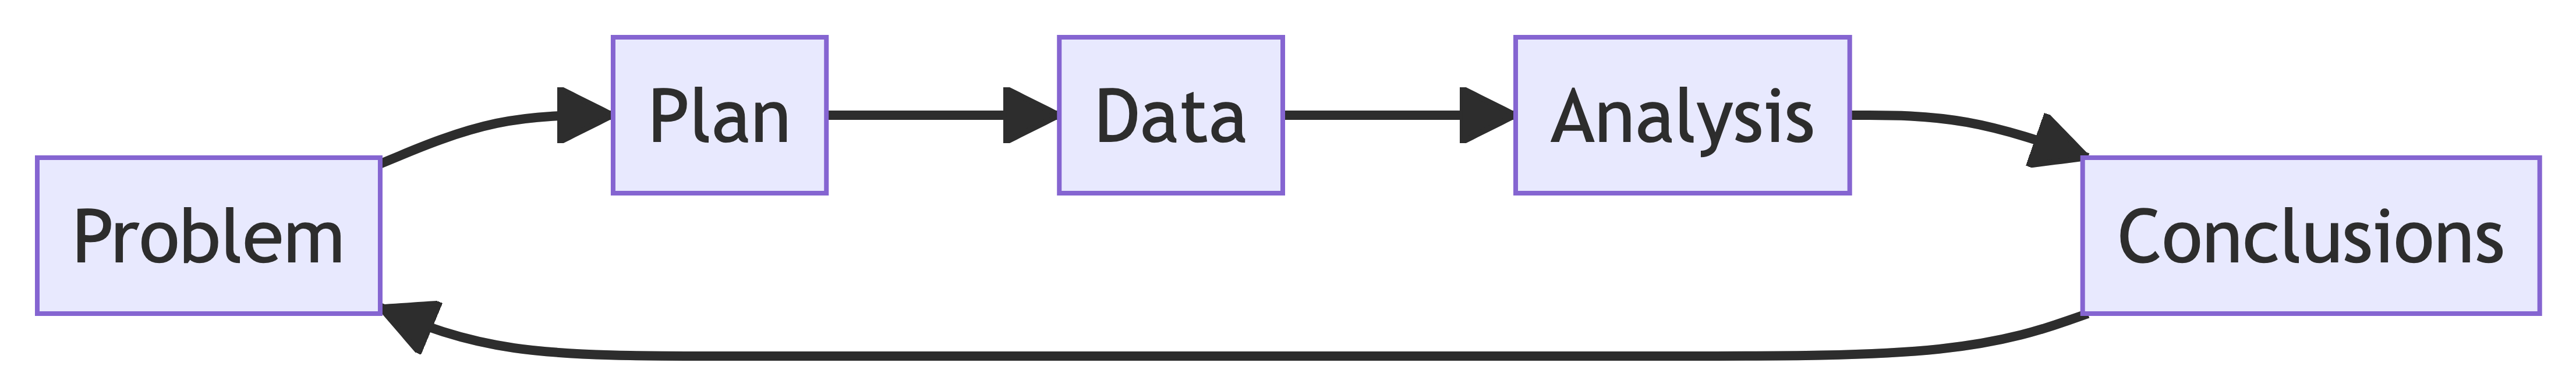
\includegraphics[width=5.76in,height=0.88in]{010-rahmen_files/figure-latex/mermaid-figure-4.png}

}

\caption{\label{fig-ppdac}Datenanalyse als Prozess: Das PPDAC-Modell}

\end{figure}%

\section{Was sind Daten?}\label{was-sind-daten}

\begin{definition}[Hallo,
Daten]\protect\hypertarget{def-daten}{}\label{def-daten}

Daten kann man als eine geordnete Folge von Zeichen
definieren.\(\square\)

\end{definition}

Daten kommen häufig in Tabellenform vor; so sind sie (oft) am besten zu
untersuchen, s. Tabelle~\ref{tbl-daten}. Die erste Spalte \texttt{id}
ist nur eine laufende Nummer. Sie dient dazu, die einzelnen
Beobachtungen (hier Studentis) identifizieren zu können und birgt
ansonsten keine Information. Beispiele für ID-Variablen sind z.B.
Matrikulationsnummer, Personalausweisnummern oder Bestellnummern.

\begin{table}

\caption{\label{tbl-daten}So sehen Daten in Form einer Tabelle aus.}

\centering{

\fontsize{12.0pt}{14.4pt}\selectfont
\begin{tabular*}{\linewidth}{@{\extracolsep{\fill}}rlr}
\toprule
id & name & note \\ 
\midrule\addlinespace[2.5pt]
1 & Anna & 1.3 \\ 
2 & Berta & 2.3 \\ 
3 & Carla & 3.0 \\ 
\bottomrule
\end{tabular*}

}

\end{table}%

\begin{example}[Daten zur Forschungsfrage
2]\protect\hypertarget{exm-daten}{}\label{exm-daten}

Hier ist ein Auszug der Daten zur Tabelle \texttt{mariokart}, s.
Tabelle~\ref{tbl-mariokart}.

\begin{longtable}[]{@{}
  >{\raggedleft\arraybackslash}p{(\columnwidth - 18\tabcolsep) * \real{0.1011}}
  >{\raggedleft\arraybackslash}p{(\columnwidth - 18\tabcolsep) * \real{0.0787}}
  >{\raggedright\arraybackslash}p{(\columnwidth - 18\tabcolsep) * \real{0.0562}}
  >{\raggedleft\arraybackslash}p{(\columnwidth - 18\tabcolsep) * \real{0.1011}}
  >{\raggedleft\arraybackslash}p{(\columnwidth - 18\tabcolsep) * \real{0.0899}}
  >{\raggedleft\arraybackslash}p{(\columnwidth - 18\tabcolsep) * \real{0.1011}}
  >{\raggedright\arraybackslash}p{(\columnwidth - 18\tabcolsep) * \real{0.1236}}
  >{\raggedleft\arraybackslash}p{(\columnwidth - 18\tabcolsep) * \real{0.1348}}
  >{\raggedright\arraybackslash}p{(\columnwidth - 18\tabcolsep) * \real{0.1348}}
  >{\raggedleft\arraybackslash}p{(\columnwidth - 18\tabcolsep) * \real{0.0787}}@{}}

\caption{\label{tbl-mariokart}Auszug aus der Tabelle mariokart}

\tabularnewline

\toprule\noalign{}
\begin{minipage}[b]{\linewidth}\raggedleft
duration
\end{minipage} & \begin{minipage}[b]{\linewidth}\raggedleft
n\_bids
\end{minipage} & \begin{minipage}[b]{\linewidth}\raggedright
cond
\end{minipage} & \begin{minipage}[b]{\linewidth}\raggedleft
start\_pr
\end{minipage} & \begin{minipage}[b]{\linewidth}\raggedleft
ship\_pr
\end{minipage} & \begin{minipage}[b]{\linewidth}\raggedleft
total\_pr
\end{minipage} & \begin{minipage}[b]{\linewidth}\raggedright
ship\_sp
\end{minipage} & \begin{minipage}[b]{\linewidth}\raggedleft
seller\_rate
\end{minipage} & \begin{minipage}[b]{\linewidth}\raggedright
stock\_photo
\end{minipage} & \begin{minipage}[b]{\linewidth}\raggedleft
wheels
\end{minipage} \\
\midrule\noalign{}
\endhead
\bottomrule\noalign{}
\endlastfoot
3 & 20 & new & 0.99 & 4.0 & 52 & standard & 1580 & yes & 1 \\
7 & 13 & used & 0.99 & 4.0 & 37 & firstClass & 365 & yes & 1 \\
3 & 16 & new & 0.99 & 3.5 & 46 & firstClass & 998 & no & 1 \\
3 & 18 & new & 0.99 & 0.0 & 44 & standard & 7 & yes & 1 \\
1 & 20 & new & 0.01 & 0.0 & 71 & media & 820 & yes & 2 \\
3 & 19 & new & 0.99 & 4.0 & 45 & standard & 270144 & yes & 0 \\

\end{longtable}

Eine Erklärung (Data-Dictionary) aller Variablen des Datensatzes
\texttt{mariokart} findet sich
\href{https://www.openintro.org/data/index.php?data=mariokart}{hier}.\footnote{\url{https://www.openintro.org/data/index.php?data=mariokart}}
\(\square\)

\end{example}

\begin{definition}[Data-Dictionary]\protect\hypertarget{def-datadict}{}\label{def-datadict}

Eine Erklärung, was die Namen einer Datentabelle bedeuten, nennt man
\emph{Code Book} or \emph{Data-Dictionary}.\(\square\)

\end{definition}

\subsection{Was ist eine Variable?}\label{was-ist-eine-variable}

\begin{definition}[Variable]\protect\hypertarget{def-var}{}\label{def-var}

Eine Variable ist ein Platzhalter, der für ein Merkmal steht, das
verschiedene Werte annehmen kann.\(\square\)

\end{definition}

Man kann sich eine Variable wie einen Behälter vorstellen, auf dem mit
einem Stift geschrieben steht, was für eine Art Inhalt darin ist, s.
Abbildung~\ref{fig-var-zuweisen}.

\begin{figure}

\centering{

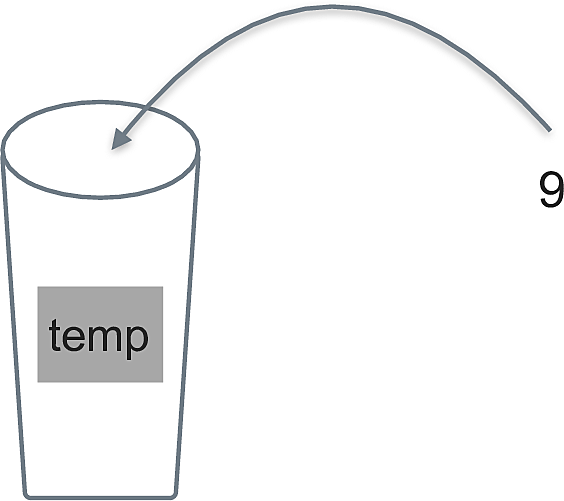
\includegraphics[width=0.25\textwidth,height=\textheight]{img/Variablen_zuweisen.png}

}

\caption{\label{fig-var-zuweisen}Wir definieren eine Variable ``temp''
mit dem Inhalt ``9''}

\end{figure}%

\subsection{Beobachtungseinheit}\label{beobachtungseinheit}

\begin{definition}[Beobachtungseinheit]\protect\hypertarget{def-beobeinheit}{}\label{def-beobeinheit}

Beobachtungseinheiten sind die Dinge, die wir untersuchen (beobachten).
Beobachtungseinheiten sind die Träger von Variablen.\(\square\)

\end{definition}

In Tabelle~\ref{tbl-daten} gibt es drei Variablen: \texttt{id},
\texttt{Name} und \texttt{Note}. Es gibt auch drei
Beobachtungseinheiten: \emph{Anna}, \emph{Berta} und \emph{Carla.}

\subsection{Wert}\label{wert}

\begin{definition}[Wert]\protect\hypertarget{def-wert}{}\label{def-wert}

Ein \emph{Wert} ist der Inhalt einer Variablen.\(\square\)

\end{definition}

In Abbildung~\ref{fig-var-zuweisen} ist der Wert von \texttt{temp} 9. In
Tabelle~\ref{tbl-daten} hat die Variable \texttt{name} drei Elemente:
Anna, Berta, Carla. Der Wert des 2. Elements ist Berta.

\begin{definition}[Ausprägung]\protect\hypertarget{def-auspraegung}{}\label{def-auspraegung}

Als \emph{Ausprägungen} bezeichnet man die verschiedenen Werte einer
Variablen. \(\square\)

\end{definition}

\begin{example}[]\protect\hypertarget{exm-geschlecht}{}\label{exm-geschlecht}

In einer Studie wurden zehn Probanden untersucht. Die Variable
\texttt{geschlecht} dokumentiert die Geschlechter der Personen:

\begin{Shaded}
\begin{Highlighting}[]
\NormalTok{geschlecht }\OtherTok{\textless{}{-}} \FunctionTok{c}\NormalTok{(}\StringTok{"Mann"}\NormalTok{, }\StringTok{"Frau"}\NormalTok{, }\StringTok{"Frau"}\NormalTok{, }\StringTok{"Frau"}\NormalTok{, }\StringTok{"Mann"}\NormalTok{,}
                \StringTok{"Frau"}\NormalTok{, }\StringTok{"Mann"}\NormalTok{, }\StringTok{"Mann"}\NormalTok{, }\StringTok{"divers"}\NormalTok{, }\StringTok{"Frau"}\NormalTok{)}
\NormalTok{geschlecht}
\DocumentationTok{\#\#  [1] "Mann"   "Frau"   "Frau"   "Frau"   "Mann"   "Frau"  }
\DocumentationTok{\#\#  [7] "Mann"   "Mann"   "divers" "Frau"}
\end{Highlighting}
\end{Shaded}

In dieser Variable (die aus 10 Werten besteht) finden sich drei
Ausprägungen: divers, Frau, Mann.\(\square\)

\end{example}

\begin{tcolorbox}[enhanced jigsaw, titlerule=0mm, left=2mm, toprule=.15mm, opacitybacktitle=0.6, breakable, bottomrule=.15mm, coltitle=black, colframe=quarto-callout-tip-color-frame, bottomtitle=1mm, title=\textcolor{quarto-callout-tip-color}{\faLightbulb}\hspace{0.5em}{Tipp}, opacityback=0, arc=.35mm, toptitle=1mm, colbacktitle=quarto-callout-tip-color!10!white, rightrule=.15mm, leftrule=.75mm, colback=white]

Gerade haben Sie etwas Computer-Syntax gesehen, genauer gesagt, Befehle
aus der Programmiersprache \emph{R}. Bisher haben wir diese Befehle
nicht kennengelernt. Sie verstehen Sie vermutlich (nicht ganz).
Ignorieren Sie diese Befehle einfach erstmal.

\end{tcolorbox}

\subsection{Tidy Data}\label{tidy-data}

\begin{definition}[Tidy
Data]\protect\hypertarget{def-tidy}{}\label{def-tidy}

Unter \emph{Tidy-Data} (tidy data, ``Normalform'') versteht man eine
Tabelle, in der jede Zeile eine Beobachtungseinheit darstellt, jede
Spalte eine Variable und jede Zelle der Tabelle einen Wert, s.
Abbildung~\ref{fig-tidy1}. (Zusätzlich ist noch eine ``Kopfzeile''
erlaubt, in der die Namen der Variablen stehen.)\(\square\)

\end{definition}

Tabelle~\ref{tbl-daten} ist ein Beispiel für Tidy-Data.
Abbildung~\ref{fig-tidy1} zeigt ein Sinnbild für Tidy-Data (Wickham \&
Grolemund, 2018). Und Abbildung~\ref{fig-tidy-hadley} erläutert das
Tidy-Prinzip genauer.

\begin{figure}

\begin{minipage}{0.50\linewidth}

\centering{

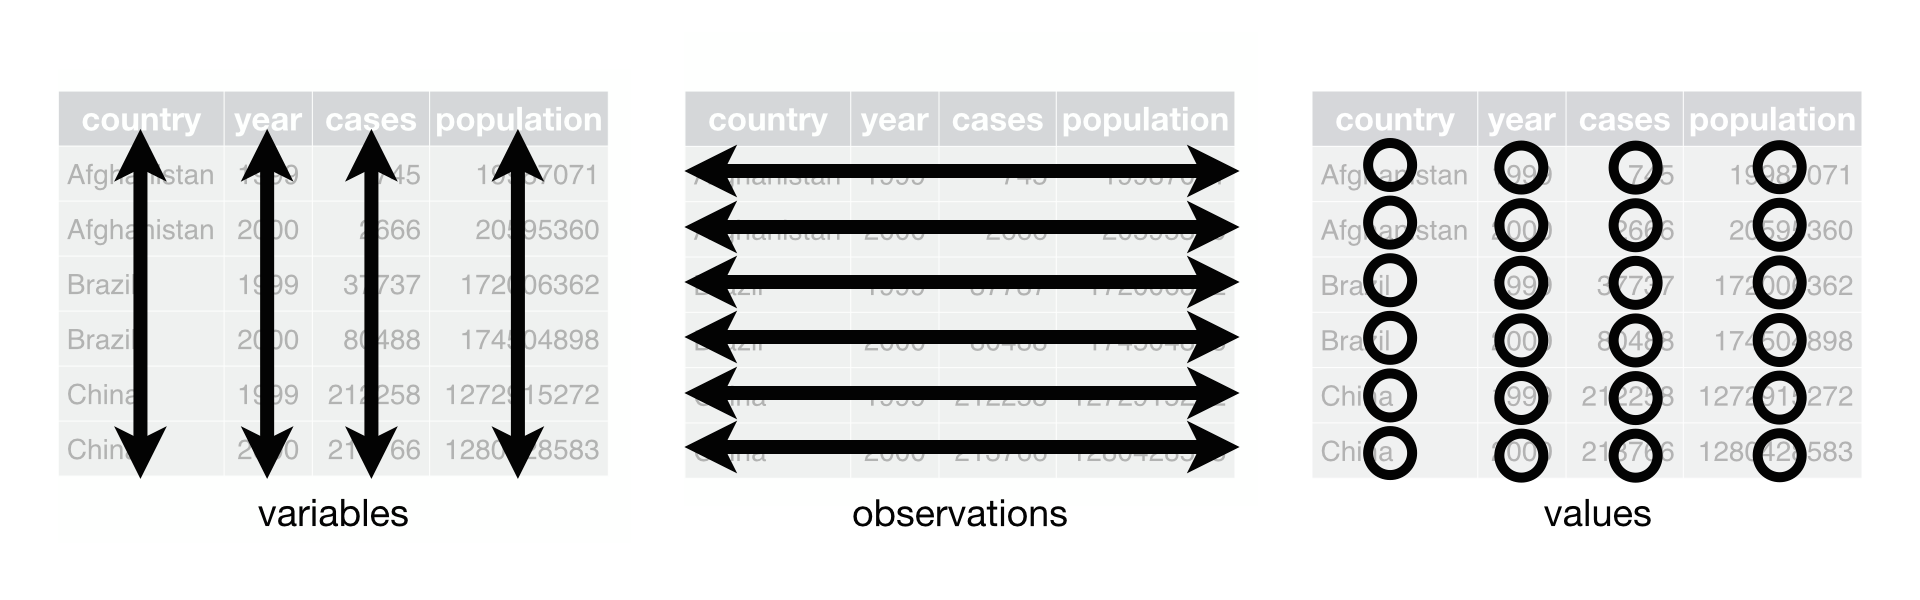
\includegraphics{img/tidy-1.png}

}

\subcaption{\label{fig-tidy1}Tidy-Data-Sinnbild (Wickham, 2023)}

\end{minipage}%
%
\begin{minipage}{0.50\linewidth}

\centering{

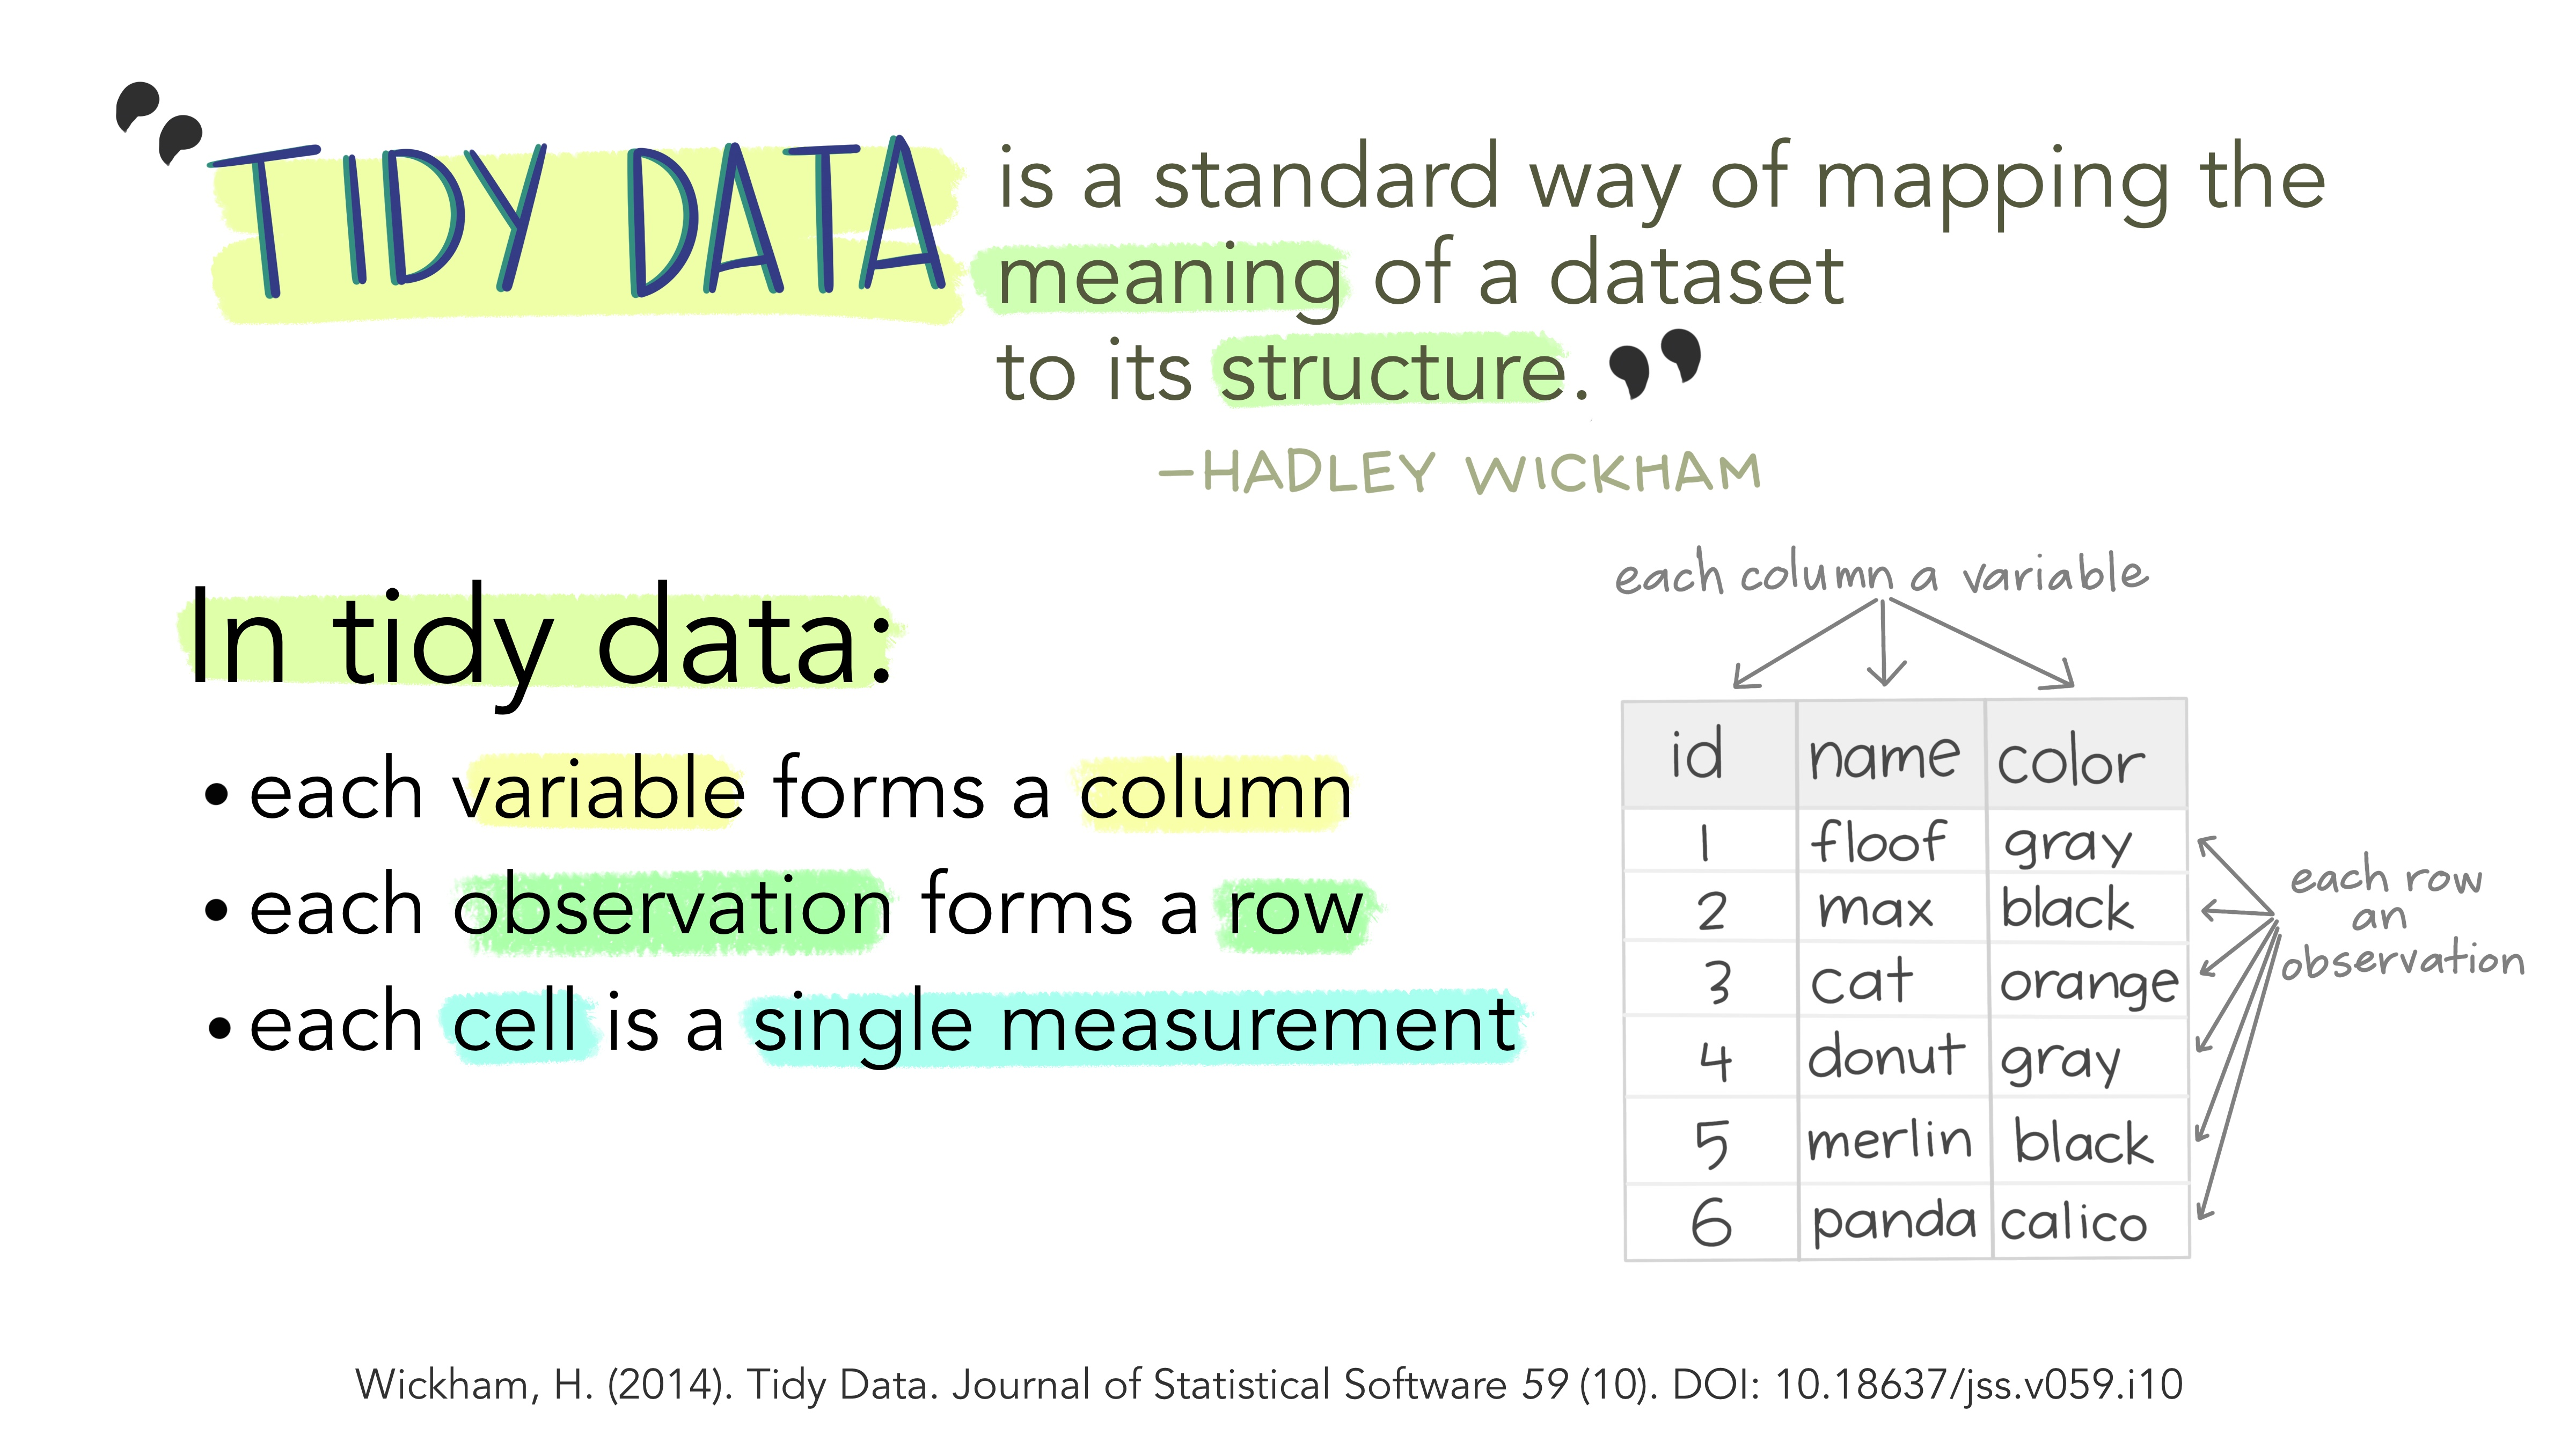
\includegraphics{img/tidydata_1.jpg}

}

\subcaption{\label{fig-tidy-hadley}Was ist Tidy-Data, fragt Horst
(2023)}

\end{minipage}%

\caption{\label{fig-tidy-all}Stay Tidy!}

\end{figure}%

\begin{tcolorbox}[enhanced jigsaw, titlerule=0mm, left=2mm, toprule=.15mm, opacitybacktitle=0.6, breakable, bottomrule=.15mm, coltitle=black, colframe=quarto-callout-important-color-frame, bottomtitle=1mm, title=\textcolor{quarto-callout-important-color}{\faExclamation}\hspace{0.5em}{Wichtig}, opacityback=0, arc=.35mm, toptitle=1mm, colbacktitle=quarto-callout-important-color!10!white, rightrule=.15mm, leftrule=.75mm, colback=white]

Für eine statistische Analyse ist es oft sinnvoll, dass die Daten im
Tidy-Format vorliegen.

\end{tcolorbox}

Der Vorteil des Tidy-Formats ist es, dass man weiß, wie die Daten
aufgebaut sind. Außerdem können Statistikprogramme oft mit dieser Form
am besten umgehen, s. Abbildung~\ref{fig-tidy3}.

\begin{figure}

\centering{

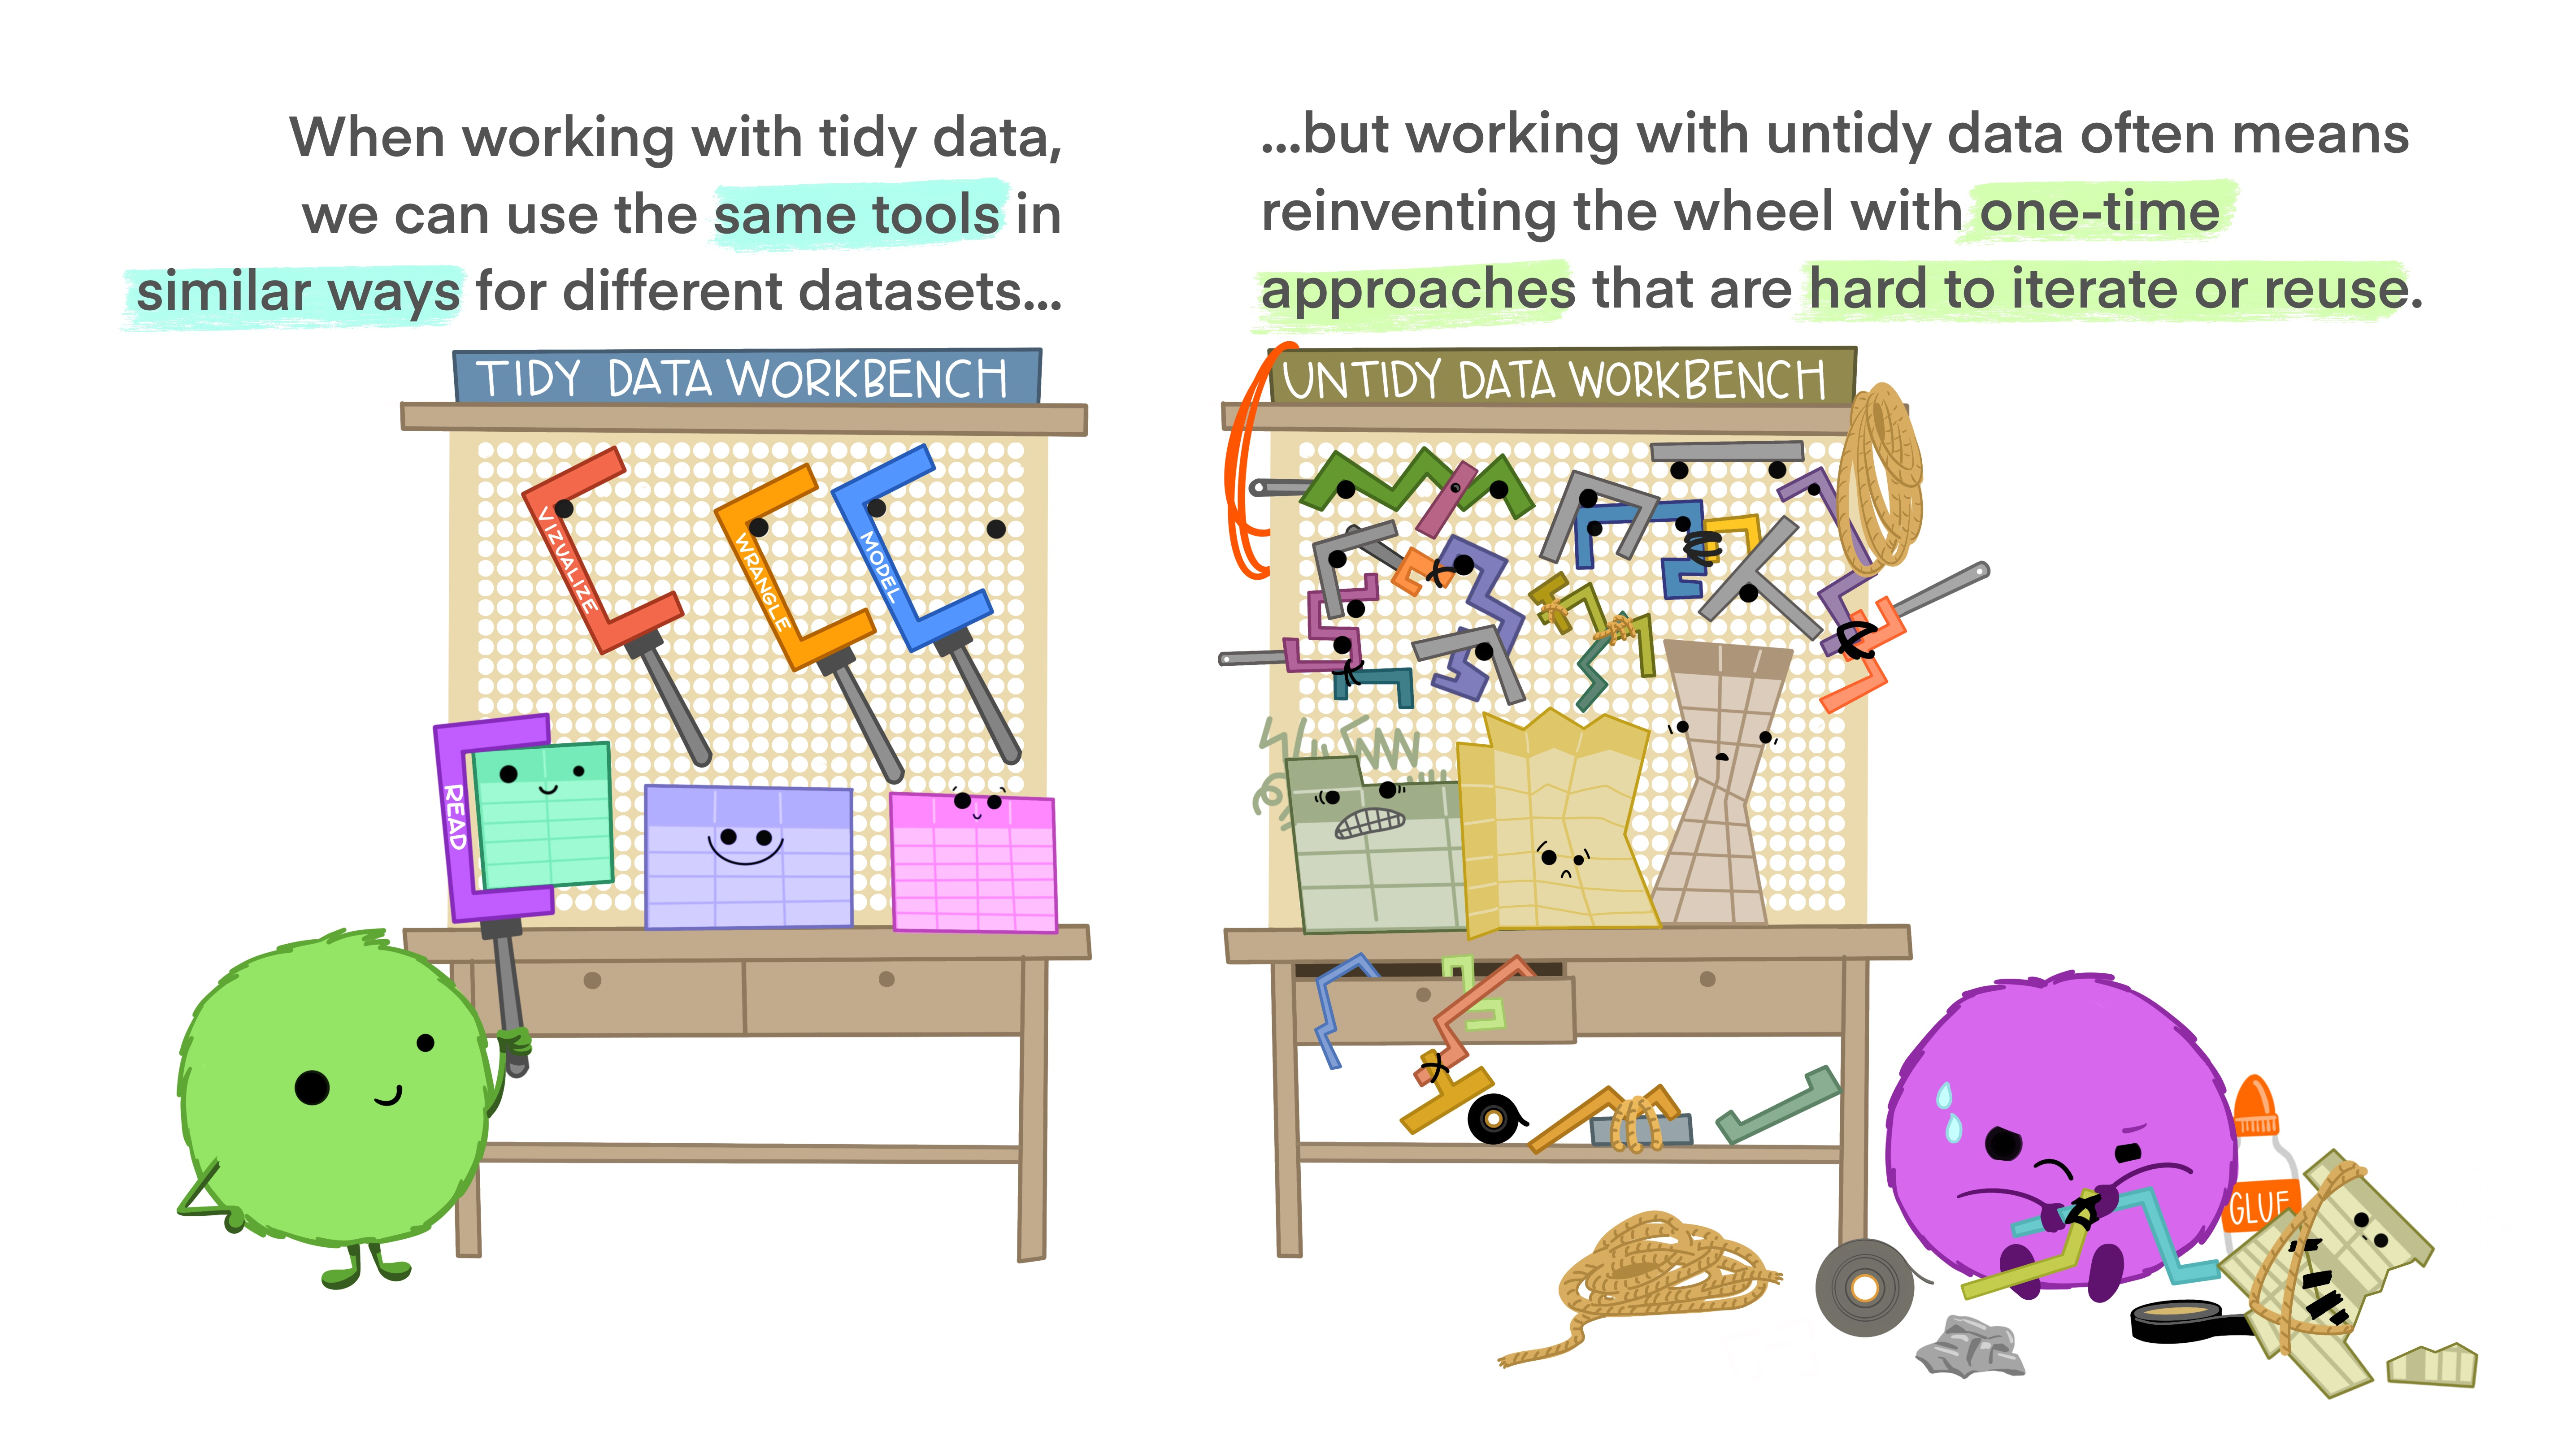
\includegraphics[width=0.75\textwidth,height=\textheight]{img/tidydata_3.jpg}

}

\caption{\label{fig-tidy3}Immer schön Ordnung halten\ldots{} (Horst,
2023)}

\end{figure}%

Das Tidy-Format wird auch als ``langes'' Format bezeichnet.

Abbildung~\ref{fig-long-wide-anim} zeigt einen Datensatz in der
``langen'' Form, also tidy, und den gleichen Datensatz, umformatiert in
der ``breiten'' Form, nicht-tidy.

\begin{figure}

\centering{

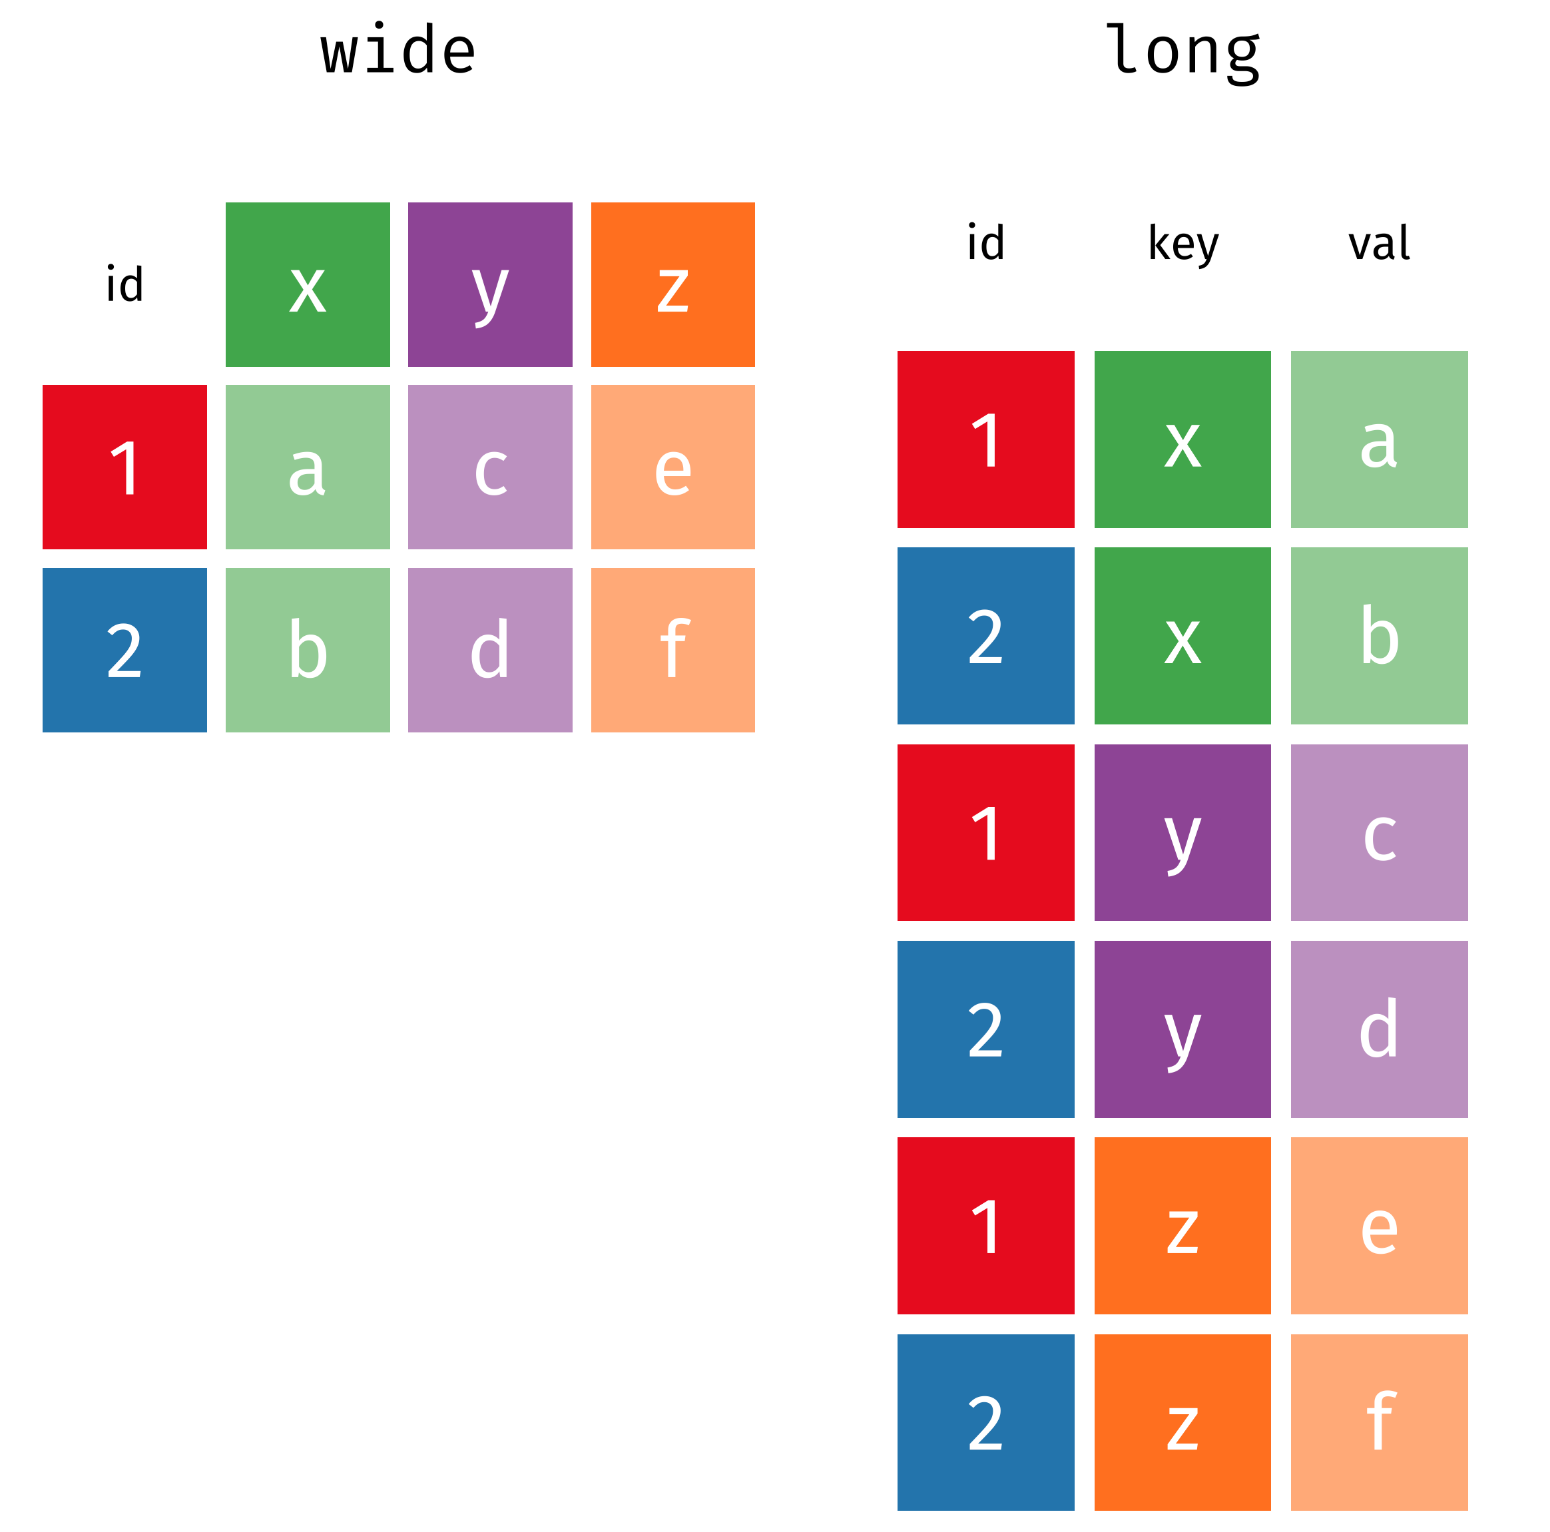
\includegraphics[width=0.5\textwidth,height=\textheight]{img/wide-long.png}

}

\caption{\label{fig-long-wide-anim}Links: Eine Tabelle mit Format
``wide'' - nicht ``tidy''. Rechts: Das ``Langformat'' (``long'') ist
``tidy''.}

\end{figure}%

\begin{example}[]\protect\hypertarget{exm-widelong}{}\label{exm-widelong}

Ihre Firmat proudziert zwei Produkte: Hämmer und Nägel. Im Folgenden
sind zwei Tabellen dargestellt, die die gleichen Informationen
darstellen: den Umsatz für die Jahre 2021 und 2022. Einmal ist dazu eine
Nicht-Tidy-Tabelle (Tabelle~\ref{tbl-untidy1}) und einmal eine
Tidy-Tabelle (Tabelle~\ref{tbl-tidy1}) verwendet. \(\square\)

\end{example}

\begin{longtable}[]{@{}lrrr@{}}

\caption{\label{tbl-untidy1}Beispiel für eine NICHT-Tidy-Tabelle
(Breitformat)}

\tabularnewline

\toprule\noalign{}
Produkt & Umsatz\_2021 & Umsatz\_2022 & Umsatz\_2023 \\
\midrule\noalign{}
\endhead
\bottomrule\noalign{}
\endlastfoot
Hämmer & 10 & 11 & 12 \\
Nägel & 15 & 10 & 5 \\

\end{longtable}

\begin{longtable}[]{@{}llr@{}}

\caption{\label{tbl-tidy1}Beispiel für eine Tidy-Tabelle (Langformat)}

\tabularnewline

\toprule\noalign{}
Produkt & Jahr & Umsatz \\
\midrule\noalign{}
\endhead
\bottomrule\noalign{}
\endlastfoot
Hämmer & 2021 & 10 \\
Hämmer & 2022 & 11 \\
Hämmer & 2023 & 12 \\
Nägel & 2021 & 15 \\
Nägel & 2022 & 10 \\
Nägel & 2023 & 5 \\

\end{longtable}

\begin{exercise}[]\protect\hypertarget{exr-widelong}{}\label{exr-widelong}

Suchen Sie ein Beispiel für eine Konfiguration einer Tabelle im Long-
vs.~Wide-Format. \(\square\)

\end{exercise}

\begin{quote}
{\emoji{student}} Wozu braucht man das Tidy-Format?
\end{quote}

\begin{quote}
{\emoji{woman-teacher}} In vielen Software-Programmen der Datenanalyse
weißt man z.B. der X- oder Y-Variable eine Spalte einer Tabelle zu.
Möchte man etwa die Veränderung des Umsatzes im Verlauf der Jahre
visualisieren oder analysieren, so braucht es die Spalten `Jahr' und
`Umsatz', also ein Tidy-Format, Tabelle~\ref{tbl-untidy1} bzw.
Tabelle~\ref{tbl-tidy1}.
\end{quote}

Abbildung~\ref{fig-tidy} stellt auf Basis einer ``Tidy-Tabelle''
(Tabelle~\ref{tbl-tidy1}) ein Diagramm dar. Ohne Tidy-Daten wäre dieses
Diagramm nicht (so einfach) zu erstellen gewesen.

\begin{figure}

\centering{

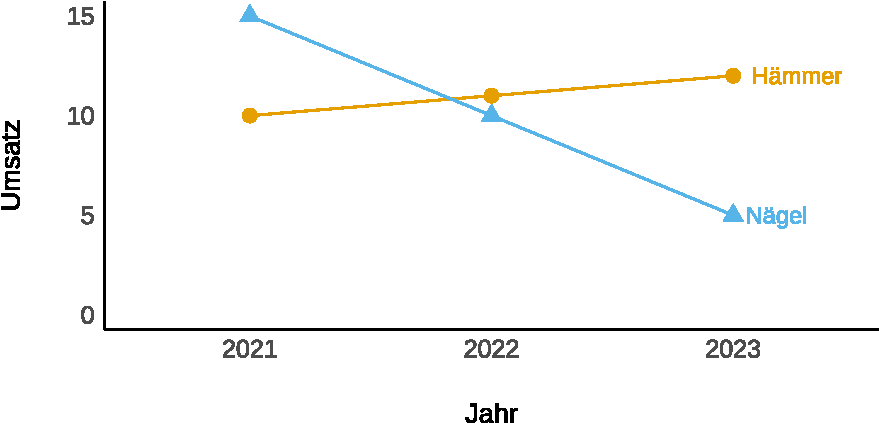
\includegraphics{010-rahmen_files/figure-pdf/fig-tidy-1.pdf}

}

\caption{\label{fig-tidy}Beispiel für eine Visualisierung auf Basis
einer Tidy-Tabelle, vgl. Tabelle~\ref{tbl-tidy1}}

\end{figure}%

\subsection{Je mehr, desto besser (?)}\label{je-mehr-desto-besser}

Was Daten betrifft, könnte man behaupten: ``Viel hilft viel'' oder ``Je
mehr, desto besser''. Natürlich unter sonst gleichen
Umständen.\footnote{Ceteris paribus, auf Latein, hört sich gleich viel
  schlauer an} Viel Datenmüll ist natürlich nicht besser als ein paar
knappe, wasserdichte Fakten!

\begin{example}[]\protect\hypertarget{exm-samplesize}{}\label{exm-samplesize}

Um Ihre eigene Lehraktivität zu organisieren, wollen Sie sich ein Bild
machen, wie viel Ihre Nebensitzerinner und Nebensitzer im Hörsaal so
lernen. Sie blicken nach links und fragen ``wie viel lernst du so?''.
Sie blicken nach recht und wiederholen die Frage gerichtet an den
Kommilitonen, der rechts neben Ihnen sitzt. Dann addieren Sie die zwei
Zahlen (unter der Annahme, dass Sie zwei Zahlen bekommen haben), und
teilen durch zwei, um den Mittelwert zu erhalten.\(\square\)

\end{example}

Ein kritischer Geist könnte anmerken, dass Sie besser die Untersuchung
nicht gemacht hätten (auch wenn Sie, vielleicht ohne zu wollen, eine
statistische Untersuchung angestellt haben). Denn bei so wenig befragten
Personen ist die Ungenauigkeit Ihrer Schätzung der typischen Lernzeit
bei Studentis einfach zu hoch.

Abbildung~\ref{fig-sample-estimate} veranschaulicht, dass man einen
Mittelwert genauer schätzen kann, wenn man auf eine größere Stichprobe
zurückgreift. Das Teilbild links zeigt den Mittelwert einer Stichprobe
mit \(n=20\) Beobachtungen. Das Teilbild rechts zeigt den Mittelwert
einer Stichprobe mit \(n=200\) Beobachtungen (jeweils aus der gleichen
Grundgesamtheit). Wie man sieht, ist im linken Teilbild die Streuung
(Variation) höher als im rechten Teilbild:

\begin{figure}

\centering{

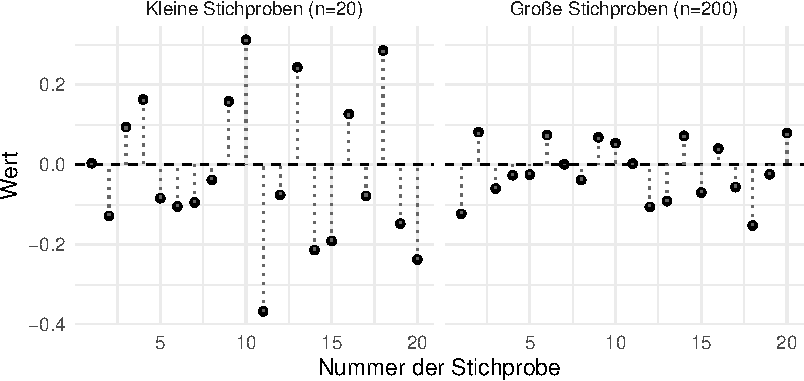
\includegraphics{010-rahmen_files/figure-pdf/fig-sample-estimate-1.pdf}

}

\caption{\label{fig-sample-estimate}Schätzgenauigkeit als Funktion der
Stichprobengröße. Jeder Punkt stellt eine Stichprobe dar, entweder mit
n=20 (links) oder mit n=200 (rechts). Kleine Stichproben (links) haben
im Schnitt eine größere Abweichung vom wahren Mittelwert als größere
Stichproben (rechts).}

\end{figure}%

\begin{tcolorbox}[enhanced jigsaw, titlerule=0mm, left=2mm, toprule=.15mm, opacitybacktitle=0.6, breakable, bottomrule=.15mm, coltitle=black, colframe=quarto-callout-important-color-frame, bottomtitle=1mm, title=\textcolor{quarto-callout-important-color}{\faExclamation}\hspace{0.5em}{Wichtig}, opacityback=0, arc=.35mm, toptitle=1mm, colbacktitle=quarto-callout-important-color!10!white, rightrule=.15mm, leftrule=.75mm, colback=white]

Mehr Daten = genauere Ergebnisse (unter sonst gleichen Umständen)
\(\square\)

\end{tcolorbox}

\begin{exercise}[Live-Experiment zum Effekt der
Stichprobengröße]\protect\hypertarget{exr-kleine-grosse-stipro}{}\label{exr-kleine-grosse-stipro}

In diesem Live-Experiment untersuchen wir den Effekt der
\emph{Stichprobengröße} auf die Streuung des Mittelwerts in der
\emph{Stichprobe.} Streuen die Ergebnisse mehr in kleinen Stichproben
als in großen? Probieren wir es aus!

In diesem Experiment werfen Sie (in kleinen Gruppen) eine Münze (auf
faire Art und Weise) und notieren das Ergebnis (Kopf oder Zahl). Uns
interessiert dabei die Frage, ob die Ergebnisse bei kleinen Stichproben
(n=5 Münzwürfe) anders streuen als in großen Stichproben (n=20
Münzwürfe).

\begin{figure}

\begin{minipage}{0.80\linewidth}
Sie brauchen nur experimentierfreudige Partner (Kleingruppen mit 2-4
Personen), eine faire Münze und dann kann's los gehen!
\href{https://docs.google.com/forms/d/e/1FAIpQLSeAwqNyZtyQwttq5JrQdQ2AO7w5vzcVDXjiejKnyFNxiWtEag/viewform?usp=sf_link}{Klicken
Sie hier, um mit dem Experiment zu starten}.\end{minipage}%
%
\begin{minipage}{0.20\linewidth}

\begin{center}

\includegraphics[width=0.75\textwidth,height=\textheight]{010-rahmen_files/figure-pdf/unnamed-chunk-16-1.pdf}
\end{center}

\end{minipage}%

\end{figure}%

Die Daten aller Versuche können Sie
\href{https://docs.google.com/spreadsheets/d/11mKFFpr-Y1CMPpq4dGA-JA_Z9jRkPbXolo54Y0G_2gE/edit?usp=sharing}{hier}
einsehen.\footnote{\url{https://tinyurl.com/3w8ke2n2}} \(\square\)

\end{exercise}

\begin{example}[Dorfschulen machen die schlauesten
Schüler!]\protect\hypertarget{exm-schule-samplesize}{}\label{exm-schule-samplesize}

In einer Pressemitteilung sei zu lesen, dass die besten Schüler in den
Dorfschulen zu finden seien (Das ist eine fiktive Geschichte). Mit etwas
Recherche finden Sie heraus, dass diese Aussage für belastbaren Daten
beruht: Tatsächlich sind die Notendurchschnitte auf den kleinen
Dorfschulen deutlich besser als in den großen Schulen in der Stadt. Also
stimmt die Behauptung der Pressemitteilung? Die gute Landluft lässt das
Hirn wachsen? Sie recherchieren noch etwas weiter in den Daten. Dann
fällt Ihnen auf: Die \emph{schlechtesten} Schüler kommen auch aus den
Dorfschulen! Eine statistische Erklärung bietet sich an: In den
Dorfschulen gibt es nur wenig Kinder und kleine Klassen -- die
Stichproben sind also klein. Bei kleinen Stichproben gibt es viel
Variation um den Mittelwert herum, s.
Abbildung~\ref{fig-sample-estimate}, und zwar nach oben (guter
Notenschnitt) und nach unten (schlechter Notenschnitt). \(\square\)

\end{example}

\section{Arten von Variablen}\label{sec-arten-variablen}

\subsection{Nach Position in der
Forschungsfrage}\label{nach-position-in-der-forschungsfrage}

Angenommen, Ihre Forschungsfrage lautet:

\begin{quote}
Hat Lernen einen Einfluss auf den Prüfungserfolg?
\end{quote}

In dem Fall gilt:

\begin{itemize}
\tightlist
\item
  \emph{Lernen} ist die Inputvariable/X-Variable/Ursache/unabhängig
  Variable (UV)
\item
  \emph{Prüfungserfolg} ist die
  Outputvariable/Y-Variable/Wirkung/abhängige Variable (AV)
\end{itemize}

Abbildung~\ref{fig-ueberblick-fragen} stellt diese beiden ``Positionen''
einer Variable dar. Die erste Position ist vor dem Pfeil. Die zweite
Position ist nach dem Pfeil.

\begin{figure}

\centering{

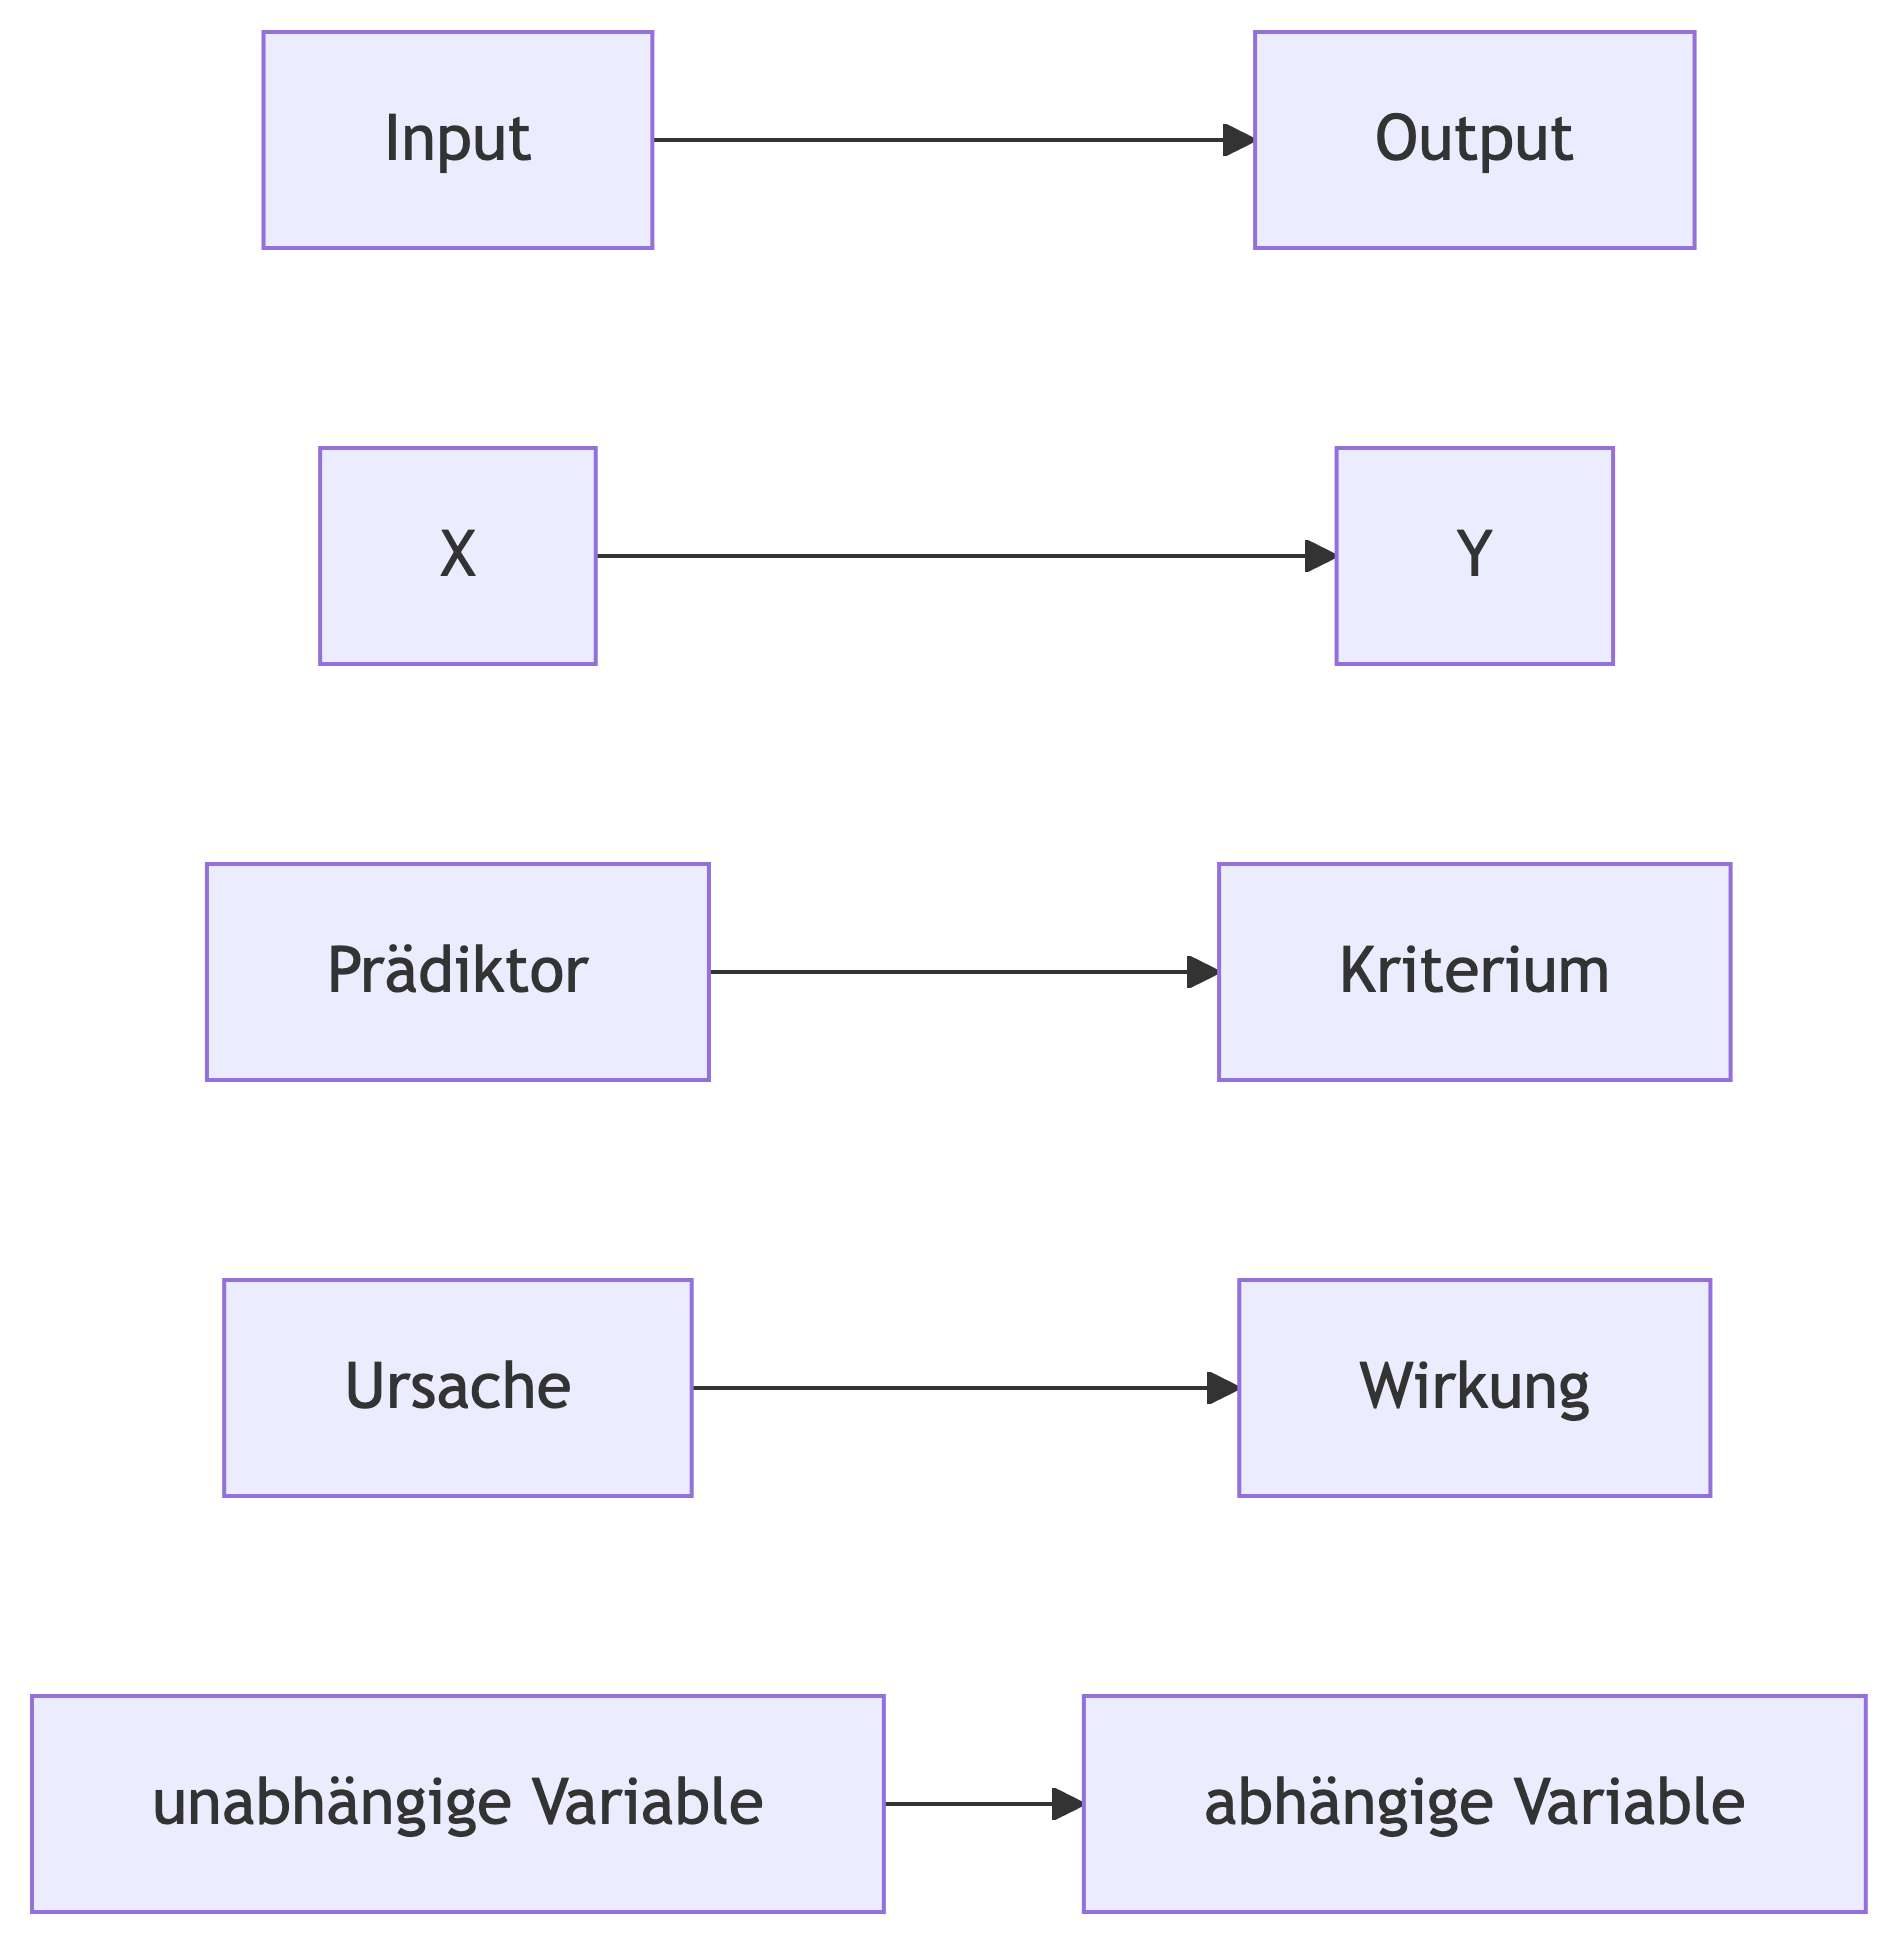
\includegraphics[width=4in,height=3.99in]{010-rahmen_files/figure-latex/mermaid-figure-3.png}

}

\caption{\label{fig-ueberblick-fragen}Synonyme Bezeichnungen für Input-
und Output-Variablen einer Forschungsfrage}

\end{figure}%

\begin{exercise}[]\protect\hypertarget{exr-uvav}{}\label{exr-uvav}

Überlegen Sie sich eine Forschungsfrage, die eine UV und eine AV
enthält. Nennen Sie einer anderen Person diese Forschungsfrage und
fragen Sie, was die UV und die AV ist. Bei richtiger Antwort belohnen
Sie großzügig. \(\square\)

\end{exercise}

\subsection{Nach dem Skalenniveau}\label{nach-dem-skalenniveau}

\begin{definition}[Skalenniveau]\protect\hypertarget{def-skalenniveau}{}\label{def-skalenniveau}

Der Begriff \emph{Skalenniveau} wird verwendet, um die Art und Menge der
Information, die in Variablen enthalten ist, zu benennen. Diese
Klassifikation basiert auf den Eigenschaften der Daten und den
mathematischen Operationen, die sinnvoll auf diese Daten angewendet
werden können. \(\square\)

\end{definition}

Abbildung~\ref{fig-skalenniveau} gibt einen Überblick über typisch
verwendete Skalenniveaus.

\begin{figure}

\centering{

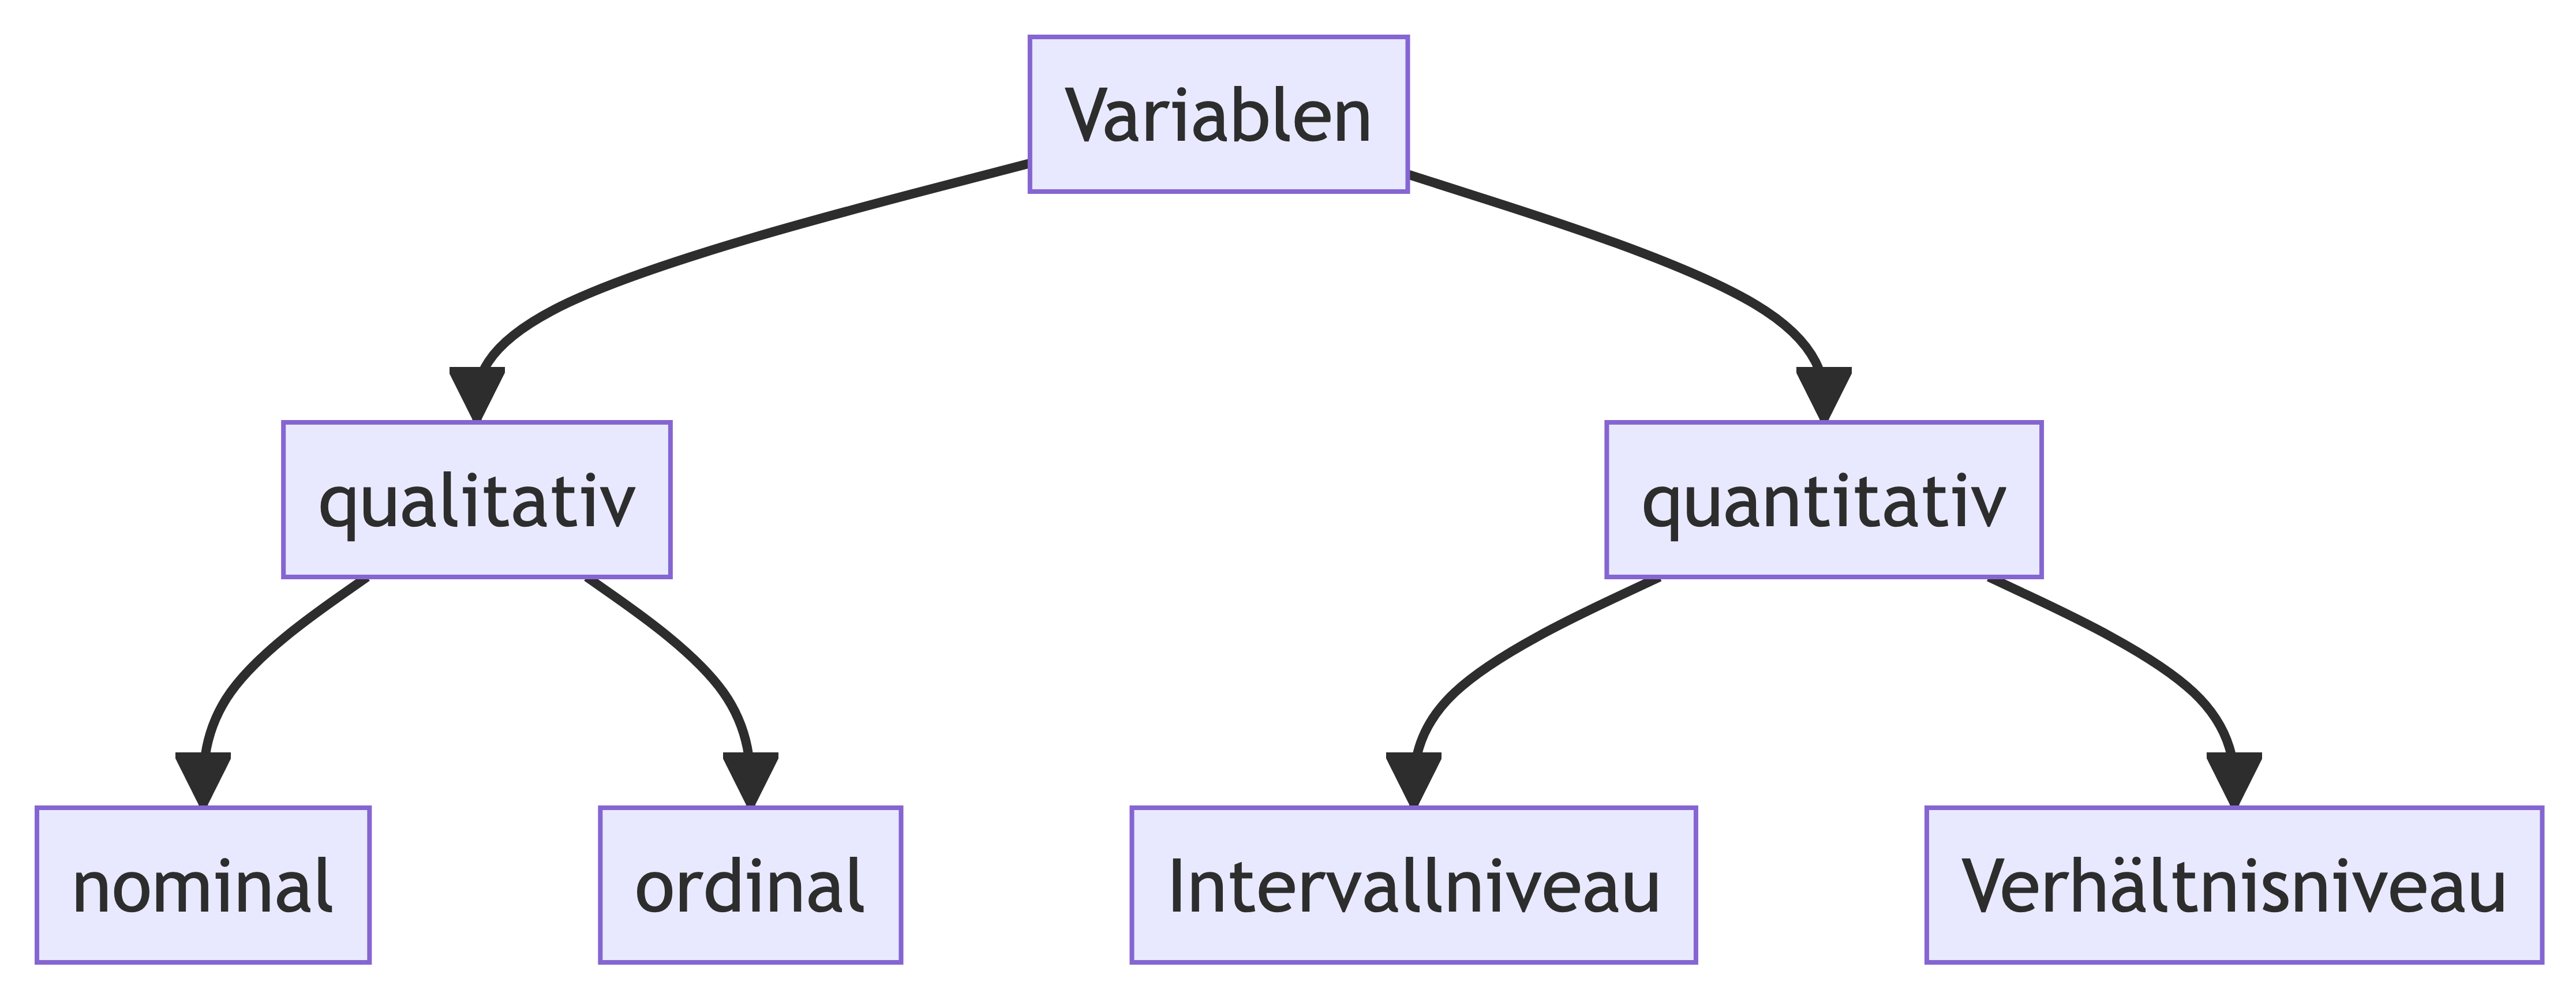
\includegraphics[width=5.82in,height=2.26in]{010-rahmen_files/figure-latex/mermaid-figure-2.png}

}

\caption{\label{fig-skalenniveau}Skalenniveaus}

\end{figure}%

\subsection{Beispiele für
Skalenniveaus}\label{beispiele-fuxfcr-skalenniveaus}

Beispiele zu den Skalenniveaus sind in Tabelle~\ref{tbl-skalen-bsps}
aufgeführt. \(\square\)

\begin{longtable}[]{@{}ll@{}}

\caption{\label{tbl-skalen-bsps}Beispiele für Skalenniveaus}

\tabularnewline

\toprule\noalign{}
Variable & Skalenniveau \\
\midrule\noalign{}
\endhead
\bottomrule\noalign{}
\endlastfoot
Haarfarbe & Nominalskala \\
Augenfarbe & Nominalskala \\
Geschlecht & Nominalskala \\
Automarke & Nominalskala \\
Partei & Nominalskala \\
Lieblingsessen & Ordinalskala \\
Medaillen beim 100-Meter-Lauf & Ordinalskala \\
Uniranking & Ordinalskala \\
IQ & Intervallskala \\
Extraversion & Intervallskala \\
Temperatur in Celcius & Intervallskala \\
Temperatur in Fahrenheit & Intervallskala \\
Temperatur in Kelvin & Verhältnisskala \\
Körpergröße & Verhältnisskala \\
Geschwindigkeit & Verhältnisskala \\
Länge & Verhältnisskala \\

\end{longtable}

Jenachdem über welches Skalenniveau eine Variable verfügt, sind
verschiedenen Rechenoperationen erlaubt, s.
{Tabelle~\ref{tbl-skalenniveaus-pdf}}.

\begin{longtable}[]{@{}
  >{\raggedright\arraybackslash}p{(\columnwidth - 10\tabcolsep) * \real{0.2237}}
  >{\raggedright\arraybackslash}p{(\columnwidth - 10\tabcolsep) * \real{0.1579}}
  >{\raggedright\arraybackslash}p{(\columnwidth - 10\tabcolsep) * \real{0.1447}}
  >{\raggedright\arraybackslash}p{(\columnwidth - 10\tabcolsep) * \real{0.1579}}
  >{\raggedright\arraybackslash}p{(\columnwidth - 10\tabcolsep) * \real{0.1184}}
  >{\raggedright\arraybackslash}p{(\columnwidth - 10\tabcolsep) * \real{0.1974}}@{}}

\caption{\label{tbl-skalenniveaus-pdf}Erlaubte Rechenoperationen nach
Skalenniveau}

\tabularnewline

\toprule\noalign{}
\begin{minipage}[b]{\linewidth}\raggedright
Skalenniveau
\end{minipage} & \begin{minipage}[b]{\linewidth}\raggedright
Quantitativ
\end{minipage} & \begin{minipage}[b]{\linewidth}\raggedright
Gleichheit
\end{minipage} & \begin{minipage}[b]{\linewidth}\raggedright
Reihenfolge
\end{minipage} & \begin{minipage}[b]{\linewidth}\raggedright
Addition
\end{minipage} & \begin{minipage}[b]{\linewidth}\raggedright
Multiplikation
\end{minipage} \\
\midrule\noalign{}
\endhead
\bottomrule\noalign{}
\endlastfoot
Nominalniveau & nein & ja & nein & nein & nein \\
Ordinalniveau & nein & ja & ja & nein & nein \\
Intervallniveau & ja & ja & ja & ja & nein \\
Verhältnisniveau & ja & ja & ja & ja & ja \\

\end{longtable}

Was soll das bedeuten, ``Rechenoperationen''? Schauen wir uns für jedes
Skalenniveau ein ``Rechenbeispiel'' an.

\emph{Nominalskala}: Die Variable \emph{Geschlecht} ist nominalskaliert.
Das bedeutet, dass ihre Ausprägungen \emph{Frau} und \emph{Mann} z.B.
nicht (sinnvoll) addiert oder sonstwie ``verrechnet'' werden können. Man
könnte, z.B. um das Eintippen zu erleichtern, Frauen mit \texttt{1}
kodieren und Männer mit \texttt{2}. Damit darf man aber nicht rechnen!
Nicht addieren, multiplizieren \ldots{} Es macht keinen Sinn zu sagen:
``Ich habe eine Frau und einen Mann in meiner Tabelle, das ist im
Schnitt ein diverses Geschlecht, weil der Mittelwert von 1 und 2 ist
1,5!'' Die \emph{einzige} ``Rechenoperation'', die man auf der
Nominalskala machen darf, ist die Prüfung auf \emph{Gleichheit}: Mann
kann feststellen, ob ein Objekt gleich zu einem anderen ist oder
unterschiedlich. Also ob zwei Personen das gleiche Geschlecht haben oder
von unterschiedlichem Geschlecht sind. Anders ausgedrückt:

\begin{itemize}
\tightlist
\item
  FRAU \(\ne\) MANN
\item
  FRAU \(=\) FRAU
\item
  MANN \(=\) MANN
\end{itemize}

\emph{Ordinalskala}: Diese Skala entspricht einer Rangordnung. Eine
Rangordnung ist etwa die geordnete Abfolge Ihres Leibgerichte (1. Pizza,
2. Spagetthi, 3. Schnitzel). Etwas ``formaler'' ausgedrückt:

\begin{itemize}
\tightlist
\item
  \(\text{Pizza} \succ \text{Spagetthi} \succ \text{Schnitzel}\)
\end{itemize}

Das komische Zeichen \(\succ\) soll heißen: ``Ist auf meiner Liste von
Leibgerichten weiter oben, mag ich lieber''. Man kann aber \emph{nicht}
sagen, ``Ich mag aber Pizza um 42\% mehr als die Spagetthi und die
wieder um 73\% mehr als ein Schnitzel!''. Zumindest kann man das nicht
ohne weitere Informationen und Annahmen. Es gibt also Dinge auf der
Welt, die man leicht in eine Rangordnung bringen kann, aber die man nur
schwer in der Größe der Unterschiede bemessen kann. Das ist die
Ordinalskala.

\begin{tcolorbox}[enhanced jigsaw, titlerule=0mm, left=2mm, toprule=.15mm, opacitybacktitle=0.6, breakable, bottomrule=.15mm, coltitle=black, colframe=quarto-callout-important-color-frame, bottomtitle=1mm, title=\textcolor{quarto-callout-important-color}{\faExclamation}\hspace{0.5em}{Wichtig}, opacityback=0, arc=.35mm, toptitle=1mm, colbacktitle=quarto-callout-important-color!10!white, rightrule=.15mm, leftrule=.75mm, colback=white]

Die Ordinalskale erlaubt, Objekte zu ordnen (hinsichtlich eines
Merkmals). Die Abstände zwischen den Objekten können nicht quantifiziert
werden. \(\square\)

\end{tcolorbox}

\emph{Intervallskala}: Das ist vielleicht eine Überraschung für Sie:
Wenn es heute 10°C hat und morgen 5°C -- dann ist es heute \emph{nicht}
doppelt so warm wie morgen. Ja, 10 ist das Doppelte von 5. Aber
\emph{10° Celcius} ist \emph{nicht} doppelt so warm wie 20° Celcius.
Wenn Sie das verwundert: Das ist normal, so geht es vielen Leuten, wenn
sie das zum ersten Mal hören. Der Grund, dass es nicht erlaubt ist,
Verhältnisse (wie doppelt/halb so viel etc.) auf der Celcius-Skala zu
bilden, ist, dass der Nullpunkt der Skala, 0° C, kein echter,
physikalischer Nullpunkt ist. Bei 0° C liegt eben nicht Null
Wärmeenergie vor. Stattdessen wurde eine Wärmenergiemenge gewählt, die
für uns Menschen ganz praktisch, da augenfällig ist: der Gefrierpunkt
von Wasser. Was bei der Intervallskala erlaubt ist, ist das Addieren
(und Subtrahieren): heute 10°C, morgen 5°C, das ist ein Unterschied von
5°C. Oder: Im Schnitt waren es 7,5°C, das ist genau in der Mitte von 5
und 10°C. Abbildung~\ref{fig-intervall} versinnbildlicht die
Intervallskala.

\begin{figure}

\centering{

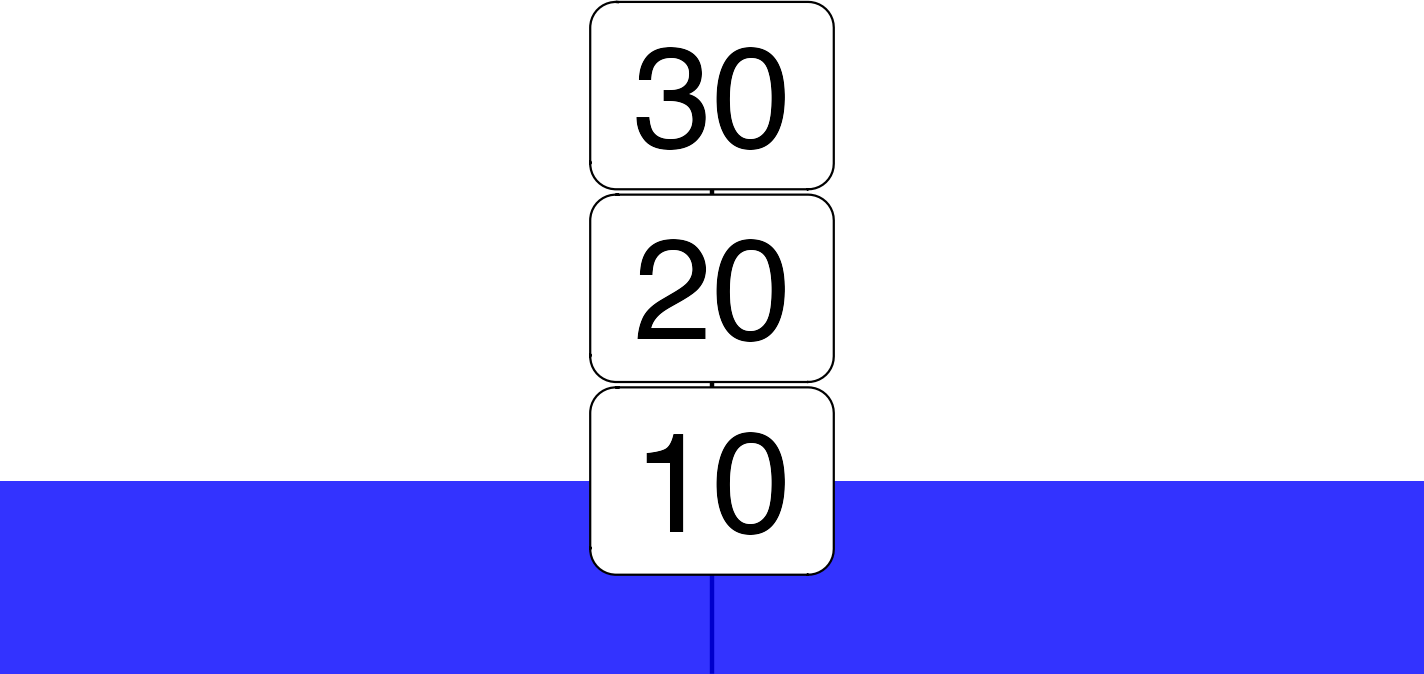
\includegraphics[width=1\textwidth,height=\textheight]{010-rahmen_files/figure-pdf/fig-intervall-1.png}

}

\caption{\label{fig-intervall}Ein Metermaß steckt im trüben Wasser. Auf
dem Metermaß können wir die aufgedruckten Zahlen ablesen. Aber wir
wissen nicht, ob der Metermaß auf dem Boden steht. Wir wissen demnach
nicht, ob der vom Metermaß angegebene Nullpunkt der wahre Nullpunkt
(Meeresboden) ist.}

\end{figure}%

\emph{Verhältnisskala}: Eine Verhältnisskala ist das, was man sich
gemeinhin unter einer metrische Variable vorstellt: Man kann ``normal''
rechnen, alle Rechenoperationen sind erlaubt. Zuzüglich zu denen, die
auch in anderen, ``niedrigeren'' Skalenniveaus erlaubt sind, ist das das
Bilden von Verhältnissen -- Multiplizieren, s.
Abbildung~\ref{fig-verhaeltnis}.

\begin{figure}

\centering{

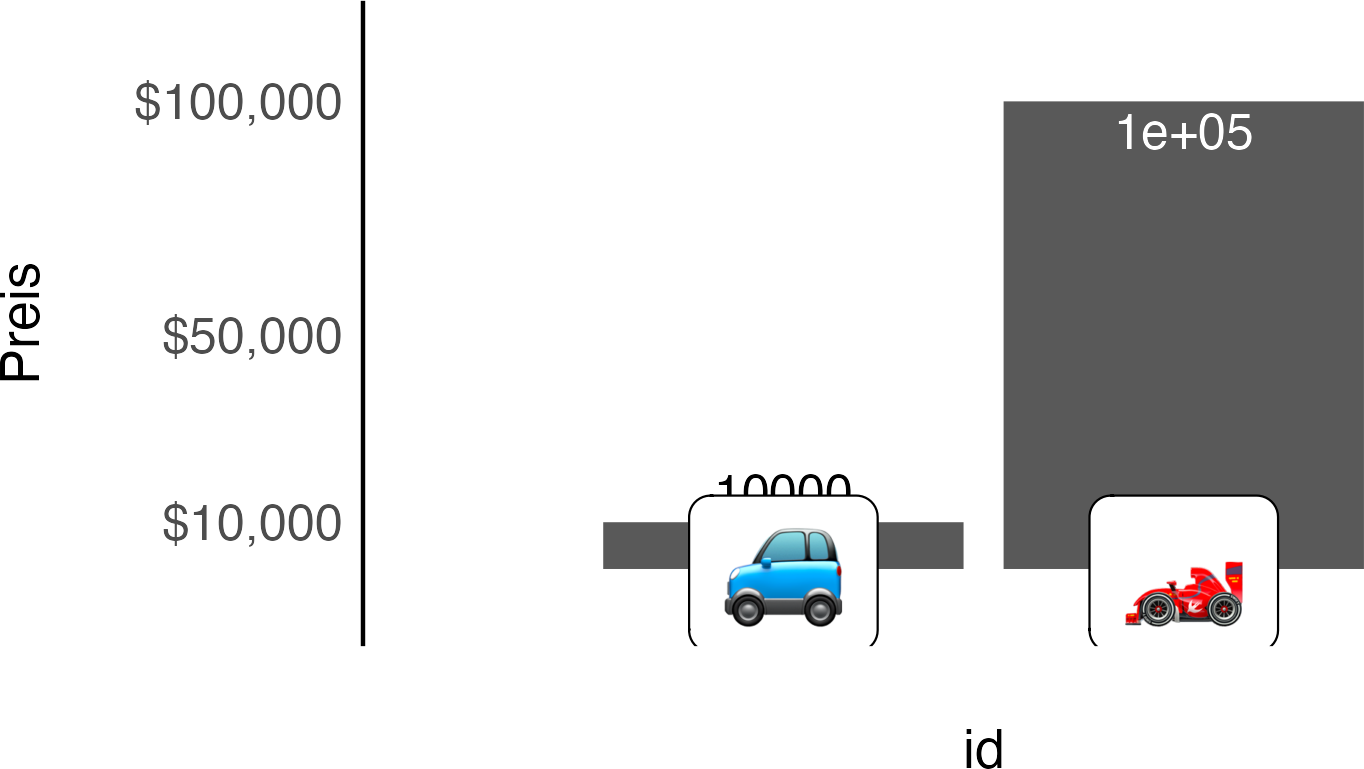
\includegraphics{010-rahmen_files/figure-pdf/fig-verhaeltnis-1.png}

}

\caption{\label{fig-verhaeltnis}Puh! Der rote Flitzer ist 10 Mal so
teuer wie die blaue Möhre. Kohlen zusammenkratzen.}

\end{figure}%

\begin{figure}

\begin{minipage}{0.80\linewidth}
In \href{https://www.youtube.com/watch?v=_mN3kFe56ng}{diesem Video} gibt
es noch ausführlichere Erklärung zum Thema Skalenniveaus.\end{minipage}%
%
\begin{minipage}{0.20\linewidth}

\begin{center}

\includegraphics[width=0.75\textwidth,height=\textheight]{010-rahmen_files/figure-pdf/unnamed-chunk-25-1.pdf}
\end{center}

\end{minipage}%

\end{figure}%

Außerdem können quantitative Variablen untergliedert werden in:

\begin{itemize}
\tightlist
\item
  \emph{stetige} Variablen, das sind Variablen, bei denen man zwischen
  zwei Ausprägungen immer noch eine weitere quetschen kann. So gibt es
  einen Wert für die Köpergröße zwischen 1.60\,m und 1.61\,m. Und einen
  Wert zwischen 1.601\,m und 1.602\,m, etc.
\item
  \emph{diskrete} Variablen, das sind metrische Variablen, die nur
  bestimmte Ausprägungen haben, häufig sind das die natürlichen Zahlen:
  \(1,2,...\). Ein Beispiel wäre die Anzahl der Kinder in einer Familie.
\end{itemize}

\begin{tcolorbox}[enhanced jigsaw, titlerule=0mm, left=2mm, toprule=.15mm, opacitybacktitle=0.6, breakable, bottomrule=.15mm, coltitle=black, colframe=quarto-callout-tip-color-frame, bottomtitle=1mm, title=\textcolor{quarto-callout-tip-color}{\faLightbulb}\hspace{0.5em}{Tipp}, opacityback=0, arc=.35mm, toptitle=1mm, colbacktitle=quarto-callout-tip-color!10!white, rightrule=.15mm, leftrule=.75mm, colback=white]

Fragen nach Skalenniveaus gehören zu den Lieblingsprüfungsfragen in
diesem Themenbereich. Sie sind gut beraten, sich gerade mit dieser Frage
intensiver zu beschäftigen. Auch in thematisch angrenzenden Fächern wird
immer wieder die Frage nach dem Skalennvieau aufgeworfen. Das zeigt
natürlich auch die hohe Relevanz des Themas.

\end{tcolorbox}

\begin{exercise}[]\protect\hypertarget{exr-skalenniveaus}{}\label{exr-skalenniveaus}

Überlegen Sie sich für einige Variablen die Skalenniveaus und befragen
Sie dann eine:n Kommilitonen dazu. \(\square\)

\end{exercise}

\section{Modelle}\label{modelle}

Woran denken Sie beim Wort ``Modell''? Vielleicht an Spielzeugautos, s.
Abbildung~\ref{fig-matchbox}.

\begin{figure}

\centering{

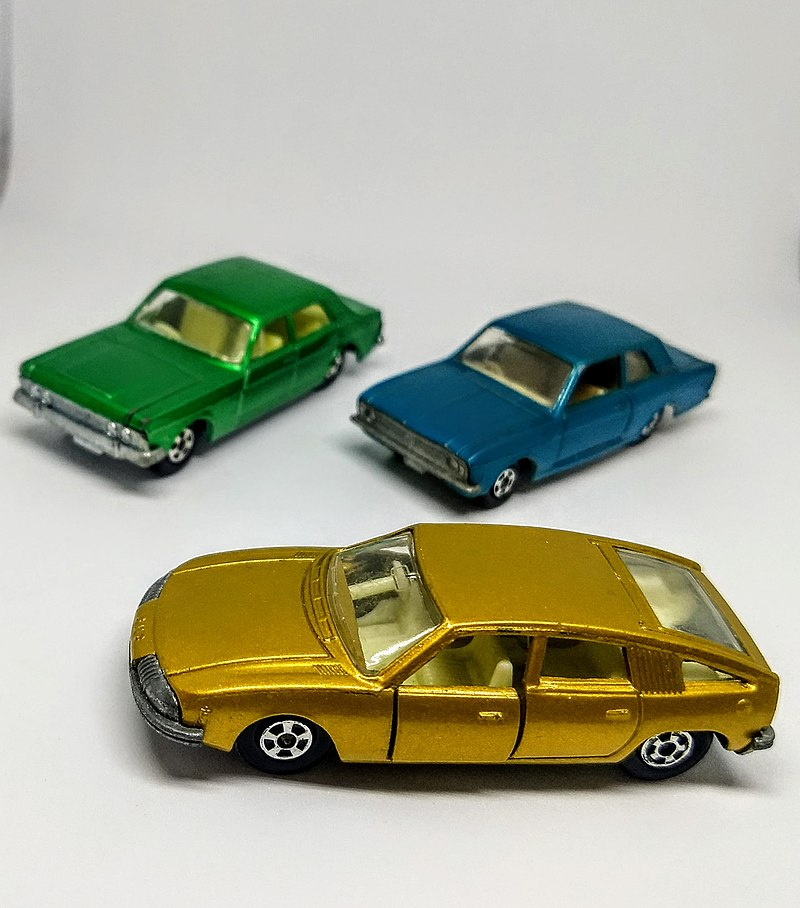
\includegraphics[width=0.25\textwidth,height=\textheight]{img/matchbox.jpg}

}

\caption{\label{fig-matchbox}Matchbox-Autos sind Modelle für Autos}

\end{figure}%

\begin{definition}[Modelle]\protect\hypertarget{def-modelle}{}\label{def-modelle}

Modelle sind ein vereinfachtes Abbild der Realität, eine
\emph{Repräsentation} (Kaplan, 2009).\(\square\)

\end{definition}

\begin{example}[Beispiele für
Modelle]\protect\hypertarget{exm-Modelle}{}\label{exm-Modelle}

Puppen sind Modelle für Babies, Landkarten für Landstriche und
\href{https://de.wikipedia.org/wiki/Bohrsches_Atommodell}{das Atommodell
von Nils Bohr} ist ein Modell für Atome.\footnote{\url{https://de.wikipedia.org/wiki/Bohrsches_Atommodell}}\(\square\)

\end{example}

Auch in der Statistik nutzen wir Modelle. Helfen Sie Prof.~Weiss-Ois: Er
blickt nicht durch. Gerne würde er wissen, wie viele Stunden seine
Studentis auf die Prüfung lernen. Aber mit so vielen Zahlen kann er
nicht umgehen \ldots{} Geben Sie ihm ein Modell: Sagen Sie ihm, wie lang
die Studis typischerweise lernen (sagen Sie ihm ein einfach den
\emph{Mittelwert} der Lernzeiten, 9.6 Stunden).

\begin{figure}

\begin{minipage}{0.46\linewidth}


\includegraphics[width=0.25\textwidth,height=\textheight]{img/teacher.png}

\subcaption{\label{}Vorher: 12, 8, 10, 11, 10, 9, 13, 9, 14, 9, 12, 14,
7, 9, 9, 11, 9, 4, 5, 12, 9, 6, 9, 12, 13, 9, 9, 6, 10\ldots{} Oh je, so
viele Zahlen! Ich check nix! Wie viel lernen denn jetzt meine Studis?!
(flaticon, 2024)}
\end{minipage}%
%
\begin{minipage}{0.09\linewidth}
~\end{minipage}%
%
\begin{minipage}{0.46\linewidth}


\includegraphics[width=0.25\textwidth,height=\textheight]{img/teacher.png}

\subcaption{\label{}Nachher: Ah, 9.6 Stunden! Yeah, jetzt weiß ich, wie
viel die Studis so typischerweise lernen. Viel zu wenig natürlich!
(flaticon, 2024)}
\end{minipage}%

\caption{\label{fig-prof}Prof.~I. Ch. Weiss-Ois hat den Mittelwert
verstanden.}

\end{figure}%

Der Nutzen von Modellen ist, dass sie komplexe Sachverhalte vereinfachen
und damit oft überhaupt erst dem Verständnis oder einer Untersuchung
zugänglich machen: Modelle ermöglichen Verständnis. In der Datenanalyse
bzw. Statistik (die beiden Begriffe werden hier weitgehend synonym
gebraucht) fassen sie oft viele Daten prägnant zusammen, z.B. zu einer
einzelnen Kennzahl. Das Verrückte an Modellen ist, dass man
Informationen wegwirft, um eine (andere, hoffentlich nützlichere)
Information zu bekommen (Stigler, 2016). Weniger ist mehr?!

\section{Praxisbezug}\label{praxisbezug}

Wir leben im Datenzeitalter; Daten durchdringen alle Bereiche des
beruflichen, gesellschaftlichen und privaten Lebens. Die Datenanalyse
hat sich in den letzten Jahren massiv verändert, da Datenmengen und
Methoden einen regelrechten Boom erlebt haben.

Diese Entwicklung ist durchaus auch kritisch zu betrachten; viele
Menschen betrachten die Entwicklung im Datenzeitalter -- Stichwort
künstliche Intelligenz -- mit Sorge. Egal ob man Daten als Segen oder
Fluch betrachtet, in beiden Fällen ist es wichtig, mit Daten umgehen zu
können. Mit der wachsenden Bedeutung von Daten wächst in gleichem Maße
die Bedeutung von Datenanalyse. Denn Daten ohne Sinn sind nutzlos. Aus
diesem Grund kann man sagen, dass Datenanalyse (und damit auch Statistik
als eine spezielle Art von Datenanalyse) zu stark nachgefragten Jobs
gehören.

\section{Wie man mit Statistik
lügt}\label{wie-man-mit-statistik-luxfcgt}

Das \emph{File-Drawer-Problem}: Sie haben ein tolles Experiment
durchgeführt, viel Arbeit, viel Stress, endlich geschafft, puh. Von den
20 Variablen (als AV, s. Kapitel~\ref{sec-arten-variablen}), die Sie
untersucht haben, zeigt nur 1 einen interessanten Effekt, leider. 1 von
20, das hört sich nicht so toll an. Wäre es da nicht ``elegant'', die 19
Variablen ohne schönen Effekt einfach in der Schublade liegen zu lassen
bis zum Sankt-Nimmerleins-Tag? Dann könnten Sie stattdessen als Ergebnis
nur die eine Variable mit schönen Ergebnis präsentieren, ganz ohne
widersprechende Befunde.

Dieser Versuchung nicht zu erliegen, kann schwer sein. Es ist aber
gefährlich, missliebige Ergebnisse zu verschweigen: Die anderen Menschen
bekommen dann ein falsches Bild der Ergebnislage; man spricht von
\href{https://de.wikipedia.org/wiki/Publikationsbias}{Publikationsbias}
(Marks‐Anglin \& Chen, 2020). Wer Ergebnisse verschweig, verzerrt die
insgesamte Befundlage (Rothstein, 2014) -- klarer Fall von
wissenschaftlichem Fehlverhalten.

\section{Fazit}\label{fazit-1}

Die Aufgabe von Statistik ist es, durch Zusammenfassen von Daten Modelle
zu bilden, die es uns einfacher machen, schwierige Sachverhalte zu
verstehen. Zentral ist dabei, die Analyse von Variabilität der Daten.
Daten kommen in verschiedenen Varianten vor, typischerweise in
Tabellenform, möglichst im Tidy-Format.

\section{Aufgaben}\label{aufgaben}

Die Webseite \href{https://datenwerk.netlify.app}{datenwerk.netlify.app}
stellt eine Reihe von einschlägigen Übungsaufgaben bereit. Sie können
die Suchfunktion der Webseite nutzen, um die Aufgaben mit den folgenden
Namen zu suchen:

\begin{enumerate}
\def\labelenumi{\arabic{enumi}.}
\tightlist
\item
  \href{https://datenwerk.netlify.app/posts/variation01/variation01.html}{variation01}
\item
  \href{https://datenwerk.netlify.app/posts/def-statistik01/def-statistik01}{Def-Statistik01}
\item
  \href{https://datenwerk.netlify.app/posts/tidy1/tidy1.html}{tidy1}
\item
  \href{https://datenwerk.netlify.app/posts/skalenniveau1a/skalenniveau1a}{Skalenniveau1a}
\item
  \href{https://datenwerk.netlify.app/posts/ziele-statistik/ziele-statistik}{Ziele-Statistik}
\item
  \href{https://datenwerk.netlify.app/posts/variation02/variation02.html}{variation02}
\item
  \href{https://datenwerk.netlify.app/posts/skalenniveau1b/skalenniveau1b}{Skalenniveau1b}
\item
  \href{https://datenwerk.netlify.app/posts/tidydata1/tidydata1.html}{tidydata1}
\end{enumerate}

\section{Vertiefung}\label{vertiefung}

\subsection{Excel für Könner}\label{excel-fuxfcr-kuxf6nner}

In vielen Organisationen werden Exceltabellen für bestimmte Zwecke der
Datenverarbeitung verwendet. Excel (und ähnliche Programme) hat
bestimmte Stärken und Vorteile, aber auch gewisse Nachteile und
Schwäche; das liegt z.T. daran, dass Excel für bestimmte Aufgaben besser
und für andere weniger gut geeignet ist. Wenn man mit Excel arbeitet,
wiederholen sich erfahrungsgemäß immer wieder die gleichen Fehler bzw.
suboptimalen Vorgehensweise zum Aufbau einer Exceltabelle.

\href{https://www.tandfonline.com/doi/full/10.1080/00031305.2017.1375989}{Dieser
Artikel} von Broman \& Woo (2018) zeigt anhand einiger praktischer
Tipps, wie man Exceltabellen so aufbaut, dass Fehler minimiert werden.

\begin{exercise}[Fassen Sie den Artikel von Broman \& Woo (2018)
zusammen]\protect\hypertarget{exr-xls-paper}{}\label{exr-xls-paper}

Die Lehrkraft teilt Sie dazu in Gruppen ein und weist jeder Gruppe einen
Abschnitt des Artikels zu. Fassen Sie das \emph{Wesentliche} (und nur
das Wesentliche) an einem geeigneten Ort zusammen (z.B. auf einem
Miro-Board). \(\square\)

\end{exercise}

\subsection{Sind wir süchtig nach dem
Handy?}\label{sind-wir-suxfcchtig-nach-dem-handy}

\begin{figure}

\begin{minipage}{0.80\linewidth}
Sind Sie süchtig nach Ihrem Handy? Lassen Sie uns eine kleine Studie
dazu (ggf. live im Hörsaal) durchführen. Füllen Sie
\href{https://forms.gle/PP8yb6Ubqq3JU78F9}{diese Umfrage} zum Thema
Smartphonse-Sucht aus (anonym und kein Muss).\end{minipage}%
%
\begin{minipage}{0.20\linewidth}

\begin{center}

\includegraphics[width=0.75\textwidth,height=\textheight]{010-rahmen_files/figure-pdf/unnamed-chunk-26-1.pdf}
\end{center}

\end{minipage}%

\end{figure}%

Kernstück der Umfrage ist die Smartphone-Sucht-Skala (Kwon et al.,
2013). Eine Studie fand, dass ca. ein Siebtel der Studierenden süchtig
nach ihrem Smartphone sind (Haug et al., 2015); demnach könnte dem Thema
eine hohe Bedeutsamkeit zukommen.

Wir werden die Daten im weiteren Verlauf auswerten. \(\square\)

\subsection{Datenprofi plaudert aus dem
Nähkästchen}\label{datenprofi-plaudert-aus-dem-nuxe4hkuxe4stchen}

Inspiration von einer Praktikerin der Datenanalyse: Caitlin Hudon verrät
\href{https://www.youtube.com/watch?v=O5lP6XcopdQ&list=PL9HYL-VRX0oQchs7dqFICoxMgnvFO10tC&index=15&t=1s}{in
diesem Video}, welche Fehler Sie sie in in den acht Jahren ihrer
Berufserfahrung gemacht hat und was sie daraus gelernt hat.\footnote{\url{https://youtu.be/O5lP6XcopdQ?si=7UsS6xbeYjnorGhx}}

\url{https://www.youtube.com/watch?v=O5lP6XcopdQ&list=PL9HYL-VRX0oQchs7dqFICoxMgnvFO10tC&index=15&t=1s}

\section{Literaturhinweise}\label{literaturhinweise}

Einen Einblick in die Fundamente statistischer Analyse bietet Stigler
(2016). Cetinkaya-Rundel \& Hardin (2021), stellen grundlegende Konzepte
der Analyse von Daten im Kapitel 1, ``Hello data'', vor. Downey (2023)
illustriert statistische Überraschungsmoment auf unterhaltsame, und vor
allem: sofataugliche Art.

\chapter{Daten einlesen}\label{daten-einlesen}

\section{Lernsteuerung}\label{lernsteuerung-1}

Abb. Abbildung~\ref{fig-ueberblick} den Standort dieses Kapitels im
Lernpfad und gibt damit einen Überblick über das Thema dieses Kapitels
im Kontext aller Kapitel.

\subsection{Lernziele}\label{lernziele-2}

\begin{itemize}
\tightlist
\item
  Sie können R und RStudio starten.
\item
  Sie können R-Pakete installieren und starten.
\item
  Sie können Variablen in R zuweisen und auslesen.
\item
  Sie können Daten in R importieren.
\item
  Sie können den Begriff \emph{Reproduzierbarkeit} definieren.
\end{itemize}

\subsection{Ab diesem Kapitel benötigen Sie
R}\label{ab-diesem-kapitel-benuxf6tigen-sie-r}

Bitte stellen Sie sicher, dass Sie R rechtzeitig einsatzbereit haben.
Weiter unten in diesem Kapitel finden Sie Installationshinweise
(Kapitel~\ref{sec-install-r}). Falls Sie dieses Kapitel zum ersten Mal
bzw. sich noch nicht mit R auskennen, werden Sie vielleicht einigen
Inhalten begegnen, die Sie noch nicht gleich verstehen. Keine Sorge, das
ist normal. Mit etwas Übung wird Ihnen bald alles schnell von der Hand
gehen.

\section{Errrstkontakt}\label{errrstkontakt}

\subsection{Warum R?}\label{warum-r}

Gründe, die für den Einsatz von R sprechen:

\begin{enumerate}
\def\labelenumi{\arabic{enumi}.}
\item
  R ist kostenlos, andere Softwarepakete für Datenanalyse sind teuer.
\item
  R und R-Befehle sind quelloffen, d.h. man kann sich die
  zugrundeliegenden Computerbefehle anschauen. Jeder kann prüfen, ob R
  vernünftig arbeitet. Alle können beitragen.
\item
  R hat die neuesten Methoden.
\item
  R hat eine große Community.
\item
  R ist maßgeschneidert für Datenanalyse.
\end{enumerate}

Allerdings gibt es auch abweichende Meinungen, s.
Abbildung~\ref{fig-bill-excel}.

\begin{figure}

\centering{


\includegraphics[width=0.5\textwidth,height=\textheight]{img/bill-gates-excel.jpg}

}

\caption{\label{fig-bill-excel}Manche finden Excel cooler als R, nicht
wahr, Bill Gates? (imgflip, 2024a)}

\end{figure}%

\subsection{R und Reproduzierbarkeit}\label{r-und-reproduzierbarkeit}

\begin{definition}[Reproduzierbarkeit]\protect\hypertarget{def-repro}{}\label{def-repro}

Ein (wissenschaftlicher) Befunde ist reproduzierbar, wenn andere
Analystis mit dem gleichen experimentellen Setup zum gleichen Ergebnis
(wie in der ursprünglichen Analyse) kommen (Plesser, 2018). \(\square\)

\end{definition}

Definition~\ref{def-repro} ist, etwas überspitzt, in
Abbildung~\ref{fig-repro} wiedergegeben.

\begin{figure}

\centering{


\includegraphics[width=0.5\textwidth,height=\textheight]{img/repro-star-struck.png}

}

\caption{\label{fig-repro}Daten + Syntax + genaue Beschreibung der
Messungen = reproduzierbar}

\end{figure}%

\begin{example}[Aus der Forschung: Reproduzierbarkeit in der
Psychologie]\protect\hypertarget{exm-repro}{}\label{exm-repro}

~

\begin{quote}
{\emoji{student}} Wie ist es um unsere Wissenschaft, Psychologie,
bestellt? Haben die Befunde Hand und Fuß?
\end{quote}

Obels et al. (2020) haben die Reproduzierbarkeit in psychologischen
Studien untersucht. Sie berichten folgendes Ergebnis

\begin{quote}
We examined data and code sharing for Registered Reports published in
the psychological literature from 2014 to 2018 and attempted to
independently computationally reproduce the main results in each
article. Of the 62 articles that met our inclusion criteria, 41 had data
available, and 37 had analysis scripts available. Both data and code for
36 of the articles were shared. We could run the scripts for 31
analyses, and we reproduced the main results for 21 articles.
\(\square\)
\end{quote}

\end{example}

\subsection{R \& RStudio}\label{r-rstudio}

Wenn wir sagen, ``wir arbeiten mit R'', dann heißt das in unserem Fall
``wir arbeiten mit R und mit RStudio''.

\begin{figure}

\begin{minipage}{0.40\linewidth}


\includegraphics[width=0.4\textwidth,height=\textheight]{img/rstudio-logo-small.png}

\subcaption{\label{}R}
\end{minipage}%
%
\begin{minipage}{0.20\linewidth}


\includegraphics[width=0.4\textwidth,height=\textheight]{img/sparkling_heart.png}

\subcaption{\label{}und}
\end{minipage}%
%
\begin{minipage}{0.40\linewidth}


\includegraphics[width=0.7\textwidth,height=\textheight]{img/rlogo.png}

\subcaption{\label{}RStudio}
\end{minipage}%

\caption{\label{fig-rlove}R und eine GUI wie RSTudio arbeiten gut
zusammen.}

\end{figure}%

Ismay \& Kim (2020) zeigen eine schöne Analogie, was der Unterschied von
\emph{R} und \emph{RStudio} ist, s. Abbildung~\ref{fig-r-rstudio}.
(Streng genommen ist RStudio für die Datenanalyse irrelevant, aber
RStudio ist praktisch, Sie werden es nicht missen wollen.)

\begin{figure}

\centering{

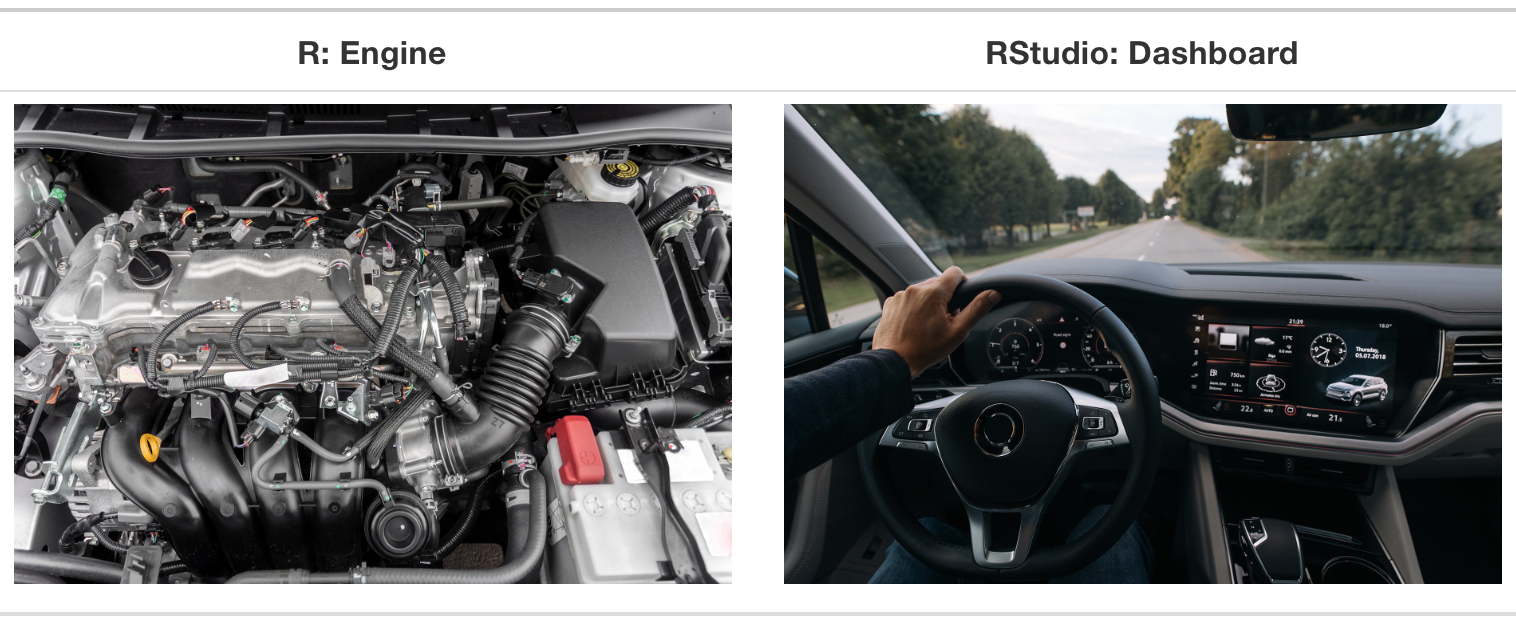
\includegraphics{img/r_vs_rstudio_1.png}

}

\caption{\label{fig-r-rstudio}R vs.~RStudio: R macht die Arbeit, RStudio
ist für Komfort und Übersicht (Ismay \& Kim, 2020).}

\end{figure}%

Kurz gesagt: Das eigentlich Arbeiten besorgt R. Für den Komfort und die
Schönheit ist RStudio zuständig. Auch eine Art von Arbeitsteilung! Hier
sehen Sie einen Screenshot von der Oberfläche von RStudio, s.
\textbf{?@fig-rstudio}.

\section{Installation von R und RStudio}\label{sec-install-r}

\subsection{Installation von R}\label{installation-von-r}

R ist ein Softwarepaket für statistische Berechnungen\footnote{Mehr
  Infos finden sich hier:
  \url{https://de.wikipedia.org/wiki/R_\%28Programmiersprache\%29}}.
Laden Sie es für Ihr Betriebssytem herunter unter
\url{https://cloud.r-project.org}.

Mehr Infos zu R finden Sie unter \url{https://cloud.r-project.org/}.
(Wenn Sie gefragt werden, dass Sie einen ``Mirror'' auswählen sollen,
heißt das, Sie sollen einen Computer (Server) wählen, von dem Sie R
herunterladen. Der sollte möglichst nicht zu weit weg stehen, dann spart
es vielleicht etwas Zeit und Bandbreite.)

Wenn Sie die Installationsdatei heruntergeladen haben, öffnen Sie diese
Datei (Doppelklick) und Sie werden durch die Installation geführt. (Sie
benötigen Admin-Rechte auf Ihrem Computer.)

\subsection{Installation von RStudio
Desktop}\label{installation-von-rstudio-desktop}

RStudio ist eine \emph{graphische Benutzeroberfläche} (graphical user
interface, GUI) für R, plus ein paar Goodies\footnote{in Form einer
  \emph{intergrierten Entwicklungsumgebung} (integrated development
  environment, IDE:
  \url{https://en.wikipedia.org/wiki/Integrated_development_environment}))}.

Laden Sie die \emph{Desktop-Version} von RStudio herunter für Ihr
Betriebssystem (Windows, MacOS, Linux) vom Anbieter (Posit) herunter.
\footnote{\url{https://posit.co/download/rstudio-desktop/}}.

Wenn Sie die Installationsdatei heruntergeladen haben, öffnen Sie diese
Datei (Doppelklick) und Sie werden durch die Installation geführt. (Sie
benötigen u.U. Admin-Rechte auf Ihrem Computer.)

\subsection{RStudio Cloud}\label{rstudio-cloud}

\subsubsection{RStudio Cloud als Alternative zu
RStudio}\label{rstudio-cloud-als-alternative-zu-rstudio}

RStudio Cloud (\url{https://rstudio.cloud/}), neuerdings auch ``Posit
Cloud'' genannt, ist ein Webdienst von Posit/RStudio (zum Teil
kostenlos), also \emph{RStudio online}: Man kann damit online mit R
arbeiten. Die Oberfläche ist praktisch identisch zur Desktop-Version, s.
Abbildung~\ref{fig-rstudio-cloud}. Sie können es als Alternative zur
Installation von RStudio auf Ihrem Computer verwenden. Ein Vorteil von
RStudio Cloud ist, dass man als Nutzer \emph{nichts installieren} muss
und dass es \emph{auch auf Tablets} läuft (im Gegensatz zur
Desktop-Version von RStudio). Ein Nachteil ist, dass es etwas langsamer
ist und nur für ein gewisses Zeitvolumen kostenlos. Sie müssen sich ein
Konto anlegen, um den Dienst nutzen zu können.

\begin{figure}

\centering{

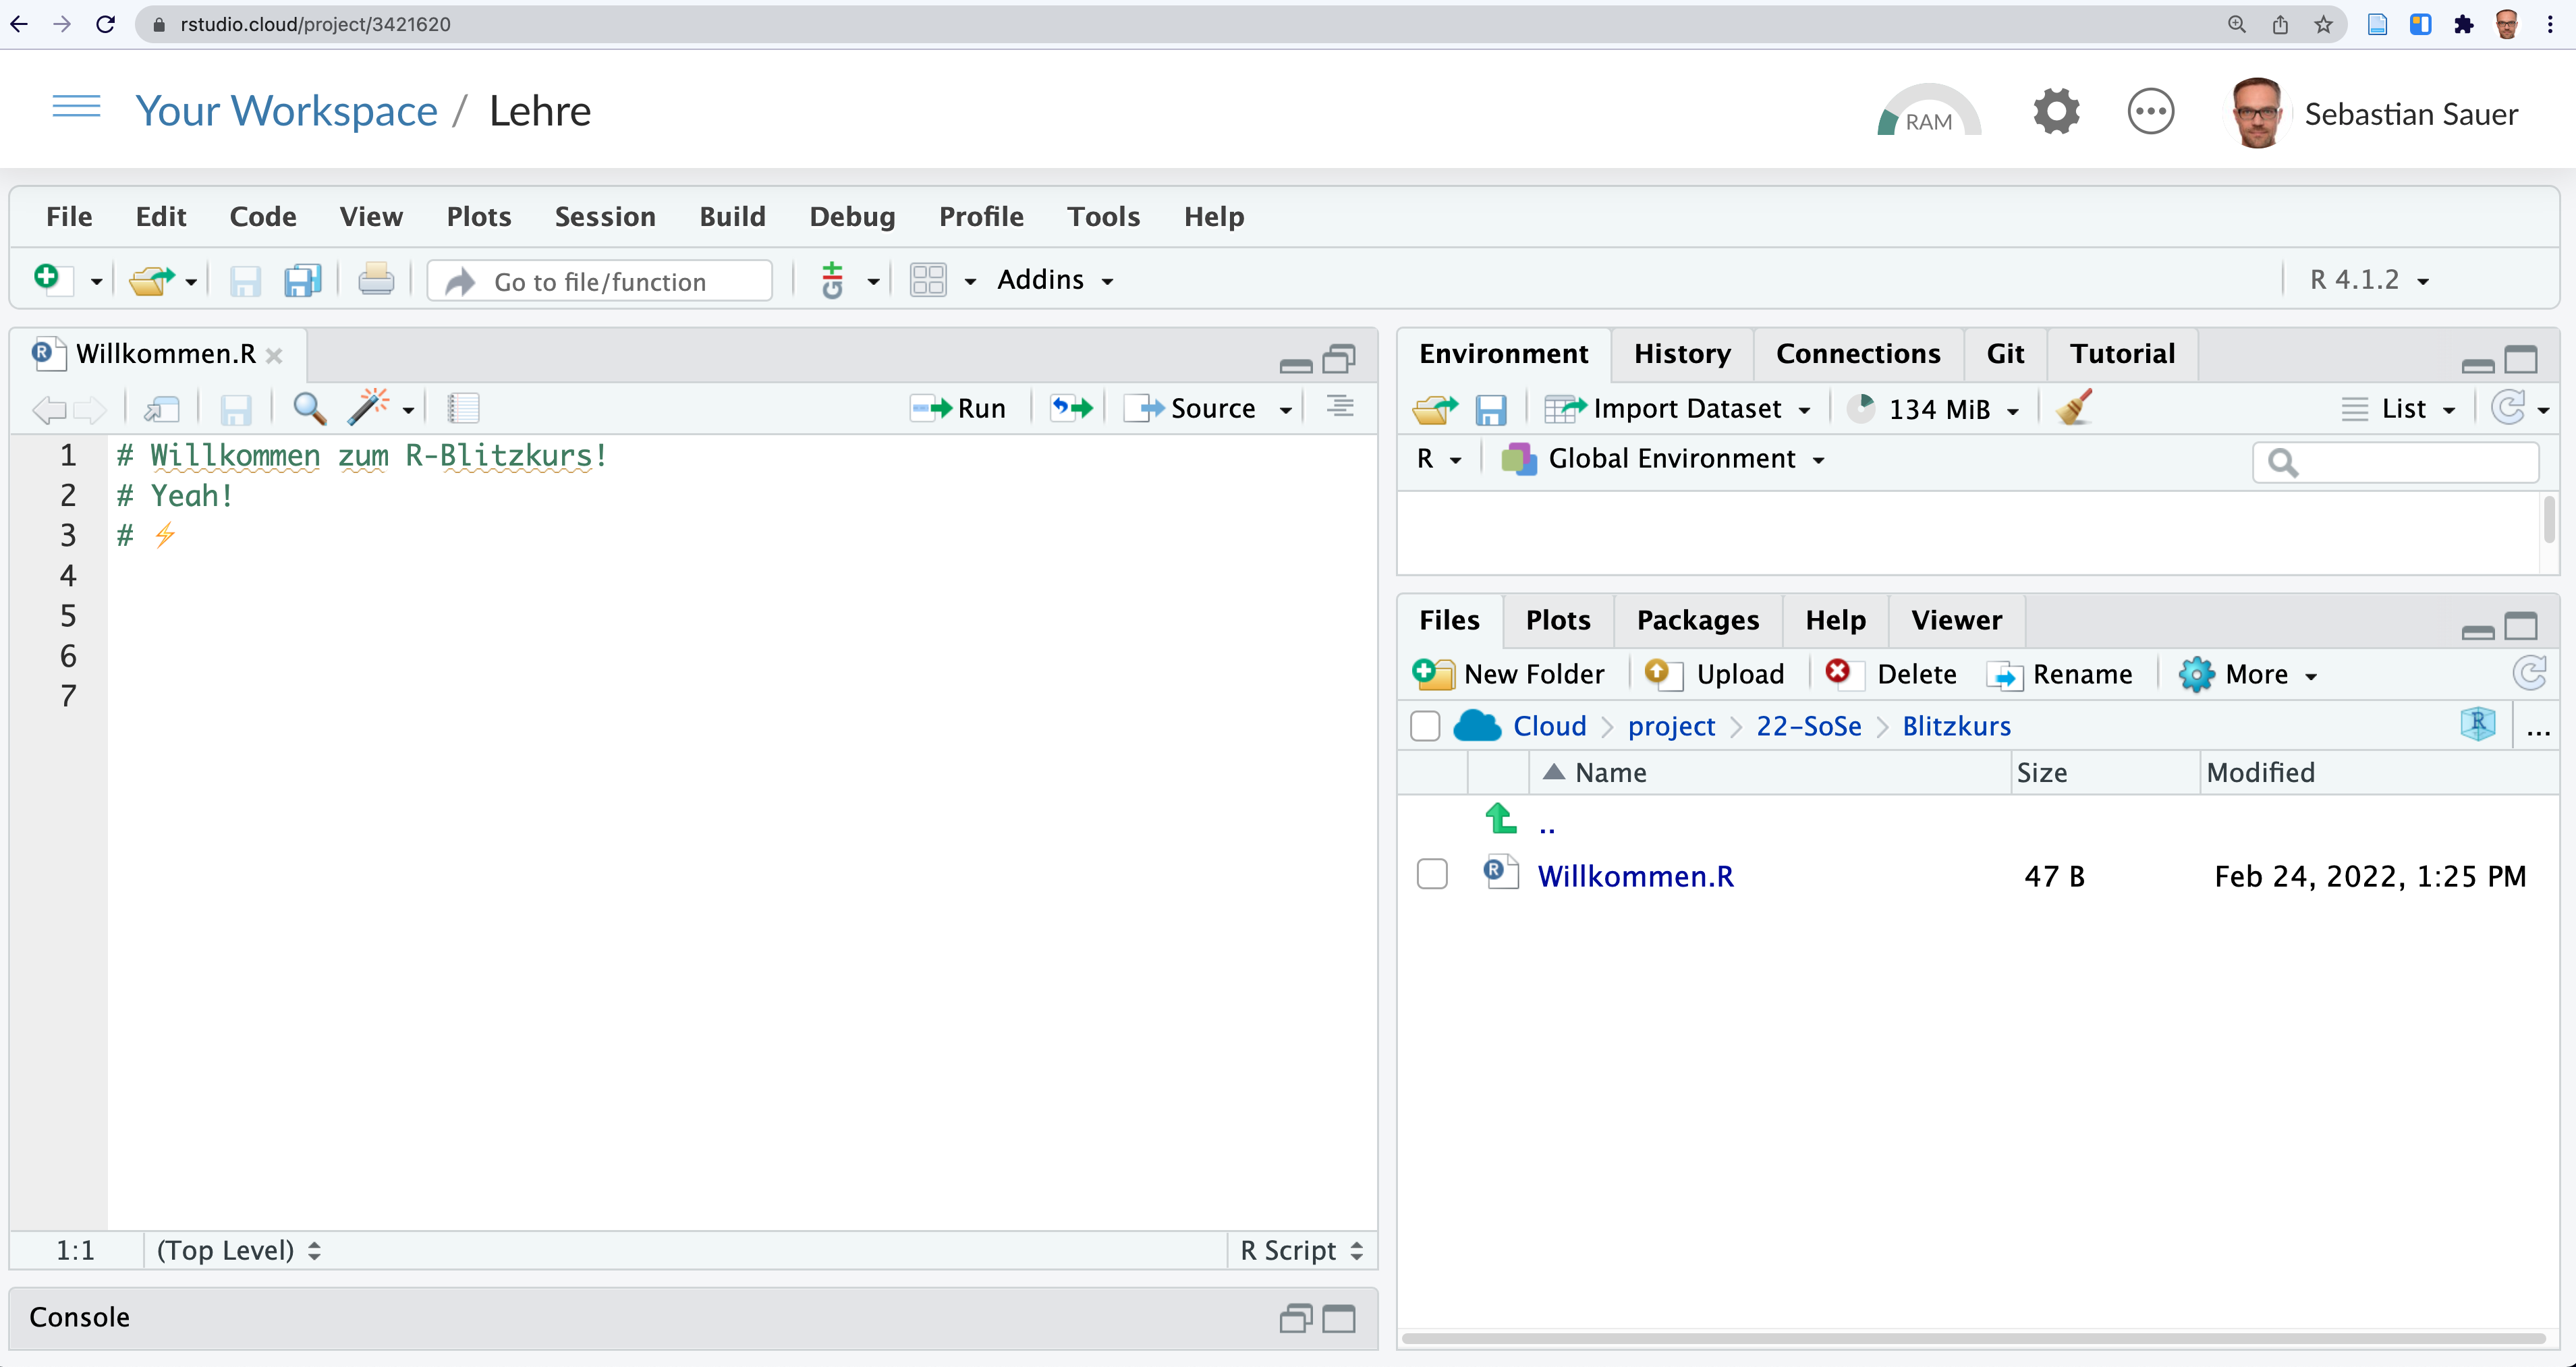
\includegraphics[width=0.75\textwidth,height=\textheight]{img/rstudio-cloud.png}

}

\caption{\label{fig-rstudio-cloud}So sieht RStudio Cloud aus. Fast genau
wie RStudio Desktop}

\end{figure}%

\subsubsection{Vertiefung}\label{vertiefung-1}

Wenn Ihr Dozent Ihnen einen Projektordner bzw. einen Link dazu
bereitstellt, ist das komfortabel, da der Dozent dann schon Pakete
installieren, Daten bereitstellen und andere Nettigkeit vorbereiten kann
für Sie. Allerdings müssen Sie den Projektordner in Ihrem Konto
abspeichern, wenn Sie etwas speichern möchten, da Sie vermutlich keine
Schreibrechte im Projektordner Ihres Dozenten haben. Klicken Sie dazu
auf ``Save a permanent copy'', s. Abbildung~\ref{fig-perm-copy}.

\begin{figure}

\centering{


\includegraphics{img/rstudio-save-a-permanent-copy.png}

}

\caption{\label{fig-perm-copy}Einen Projektordner im eigenen Konto
abspeichern, um Schreibrechte zu haben}

\end{figure}%

Sie können auch von der Cloud exportieren, also Ihre Syntaxdatei
herunterladen. Klicken Sie dazu im Reiter ``Files'' auf
\texttt{More\ \textgreater{}\ Export\ ...}.

\section{RStudio starten, nicht R}\label{rstudio-starten-nicht-r}

Wir verwenden beide Programme (R und RStudio). Aber wir \emph{öffnen
nur} RStudio. RStudio findet selbständig R und öffnet dieses
``heimlich''. Öffnen Sie nicht noch extra R (sonst wäre R zweifach
geöffnet). Anstelle von \emph{RStudio Desktop} (auf Ihrem
Computer/Desktop) können Sie auch die \emph{RStudio Cloud} (die
Online-Version ) starten.

\section{R-Pakete}\label{r-pakete}

\subsection{Was sind R-Pakete?}\label{was-sind-r-pakete}

Typisch für R ist sein modularer Aufbau: Man kann eine große Zahl an
Erweiterungen (``Pakete'', engl. \emph{packages}) installieren, alle
kostenlos. In R Paketen ``wohnen'' R-Befehle, also Dinge, die R kann,
``Skills'' sozusagen. Außerdem können in R-Paketen auch Daten
bereitgestellt werden. Damit man die Inhalte eines R-Pakets nutzen kann,
muss man es zuerst installieren und dann starten. Man kann sich daher
ein R-Paket vorstellen wie ein Buch: Wenn R es gelesen hat, dann kennt
es die Inhalte. Diese Inhalte könnten irgendwelche Formeln, also
Berechnungen sein. Es könnte aber die ``Bauanleitung'' für ein schönes
Diagramm sein. Ist ein spezielles R-Paket auf Ihrem Computer
installiert, so können Sie diese Funktionalität nutzen.

\emph{Erweiterungen} kennt man von vielen Programmen, sie werden auch
\emph{Add-Ons}, \emph{Plug-Ins} oder sonstwie genannt. Man siehe zur
Verdeutlichung Erweiterungen beim Broswer Chrome,
Abbildung~\ref{fig-chrome}.

\begin{figure}

\centering{

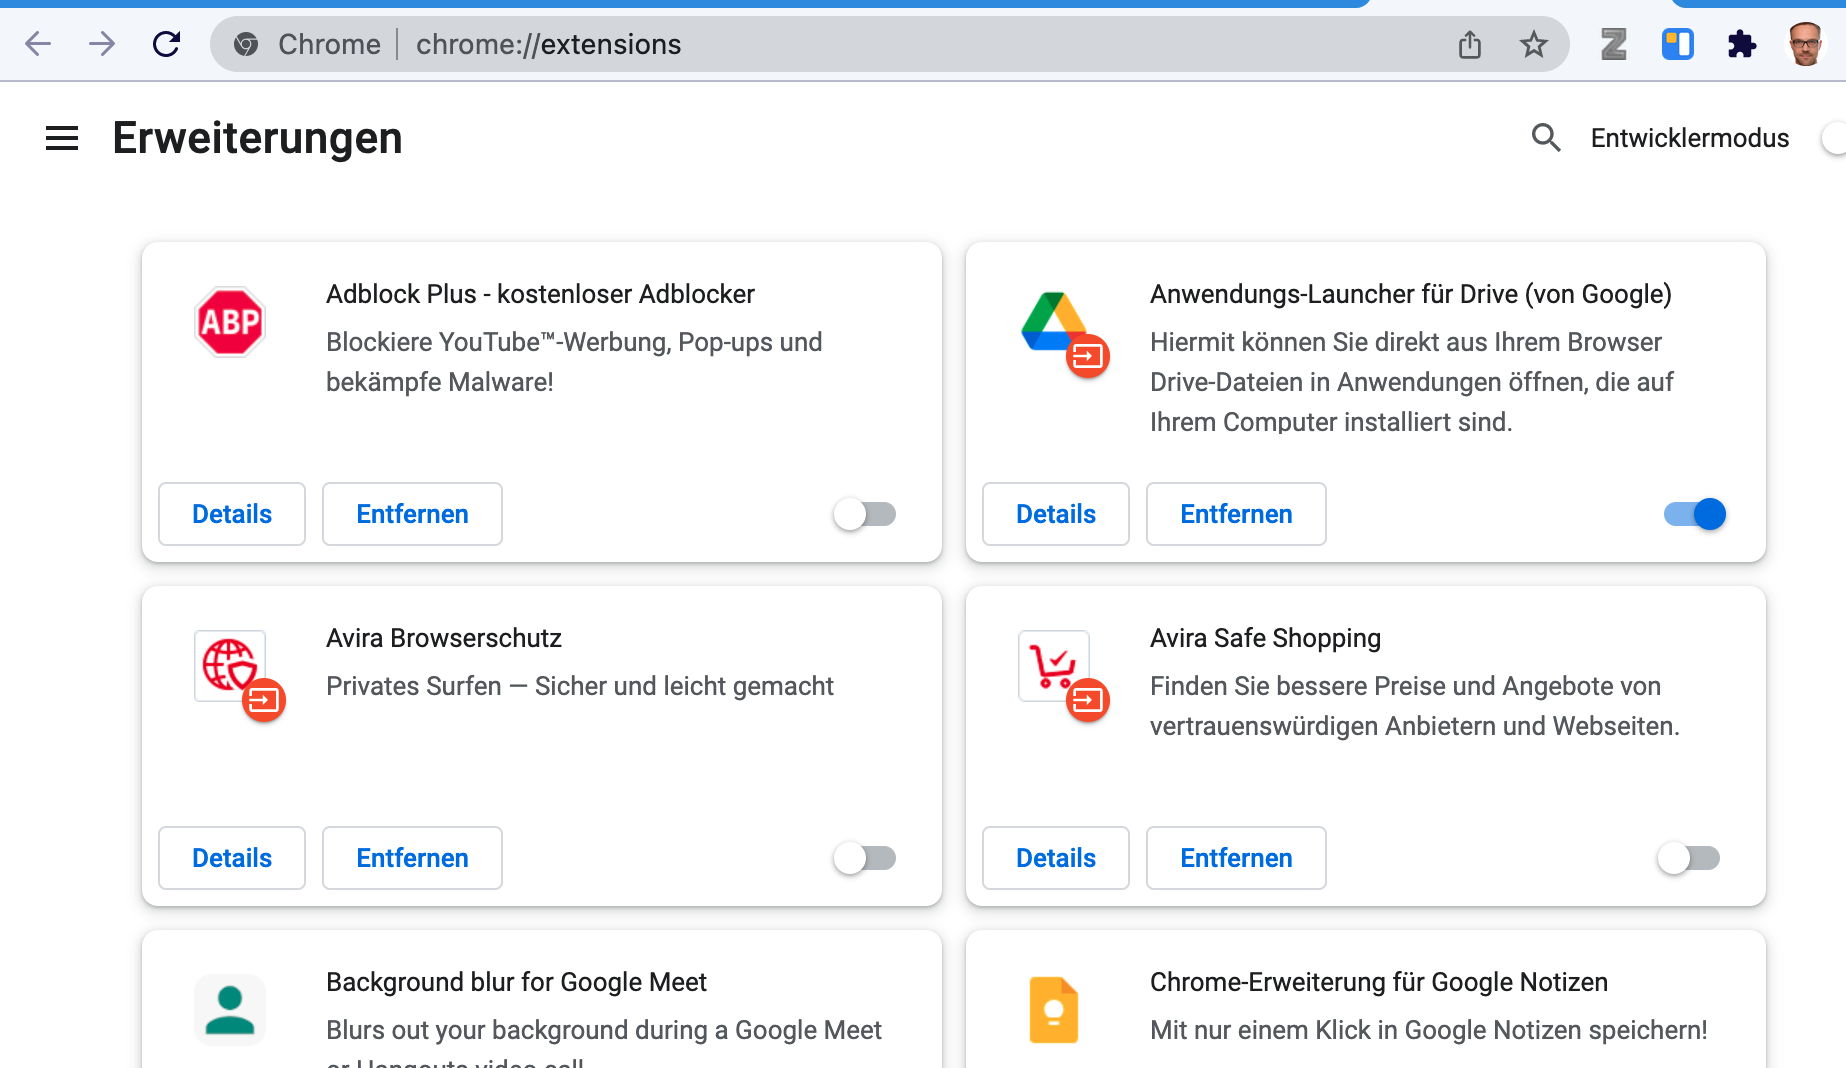
\includegraphics[width=0.5\textwidth,height=\textheight]{img/chrome-extensions.png}

}

\caption{\label{fig-chrome}Erweiterungen beim Browser Chrome}

\end{figure}%

Die Anzahl der R-Pakete ist groß; allein auf dem ``offiziellen
Web-Store'' (nennt sich ``CRAN'') von R gibt es ca. 20,000 Pakete (vgl.
Abbildung~\ref{fig-cran});
\href{https://gist.github.com/daroczig/3cf06d6db4be2bbe3368}{Stand:
2022; Quelle}). Und es kommen immer mehr dazu.

\begin{figure}

\centering{

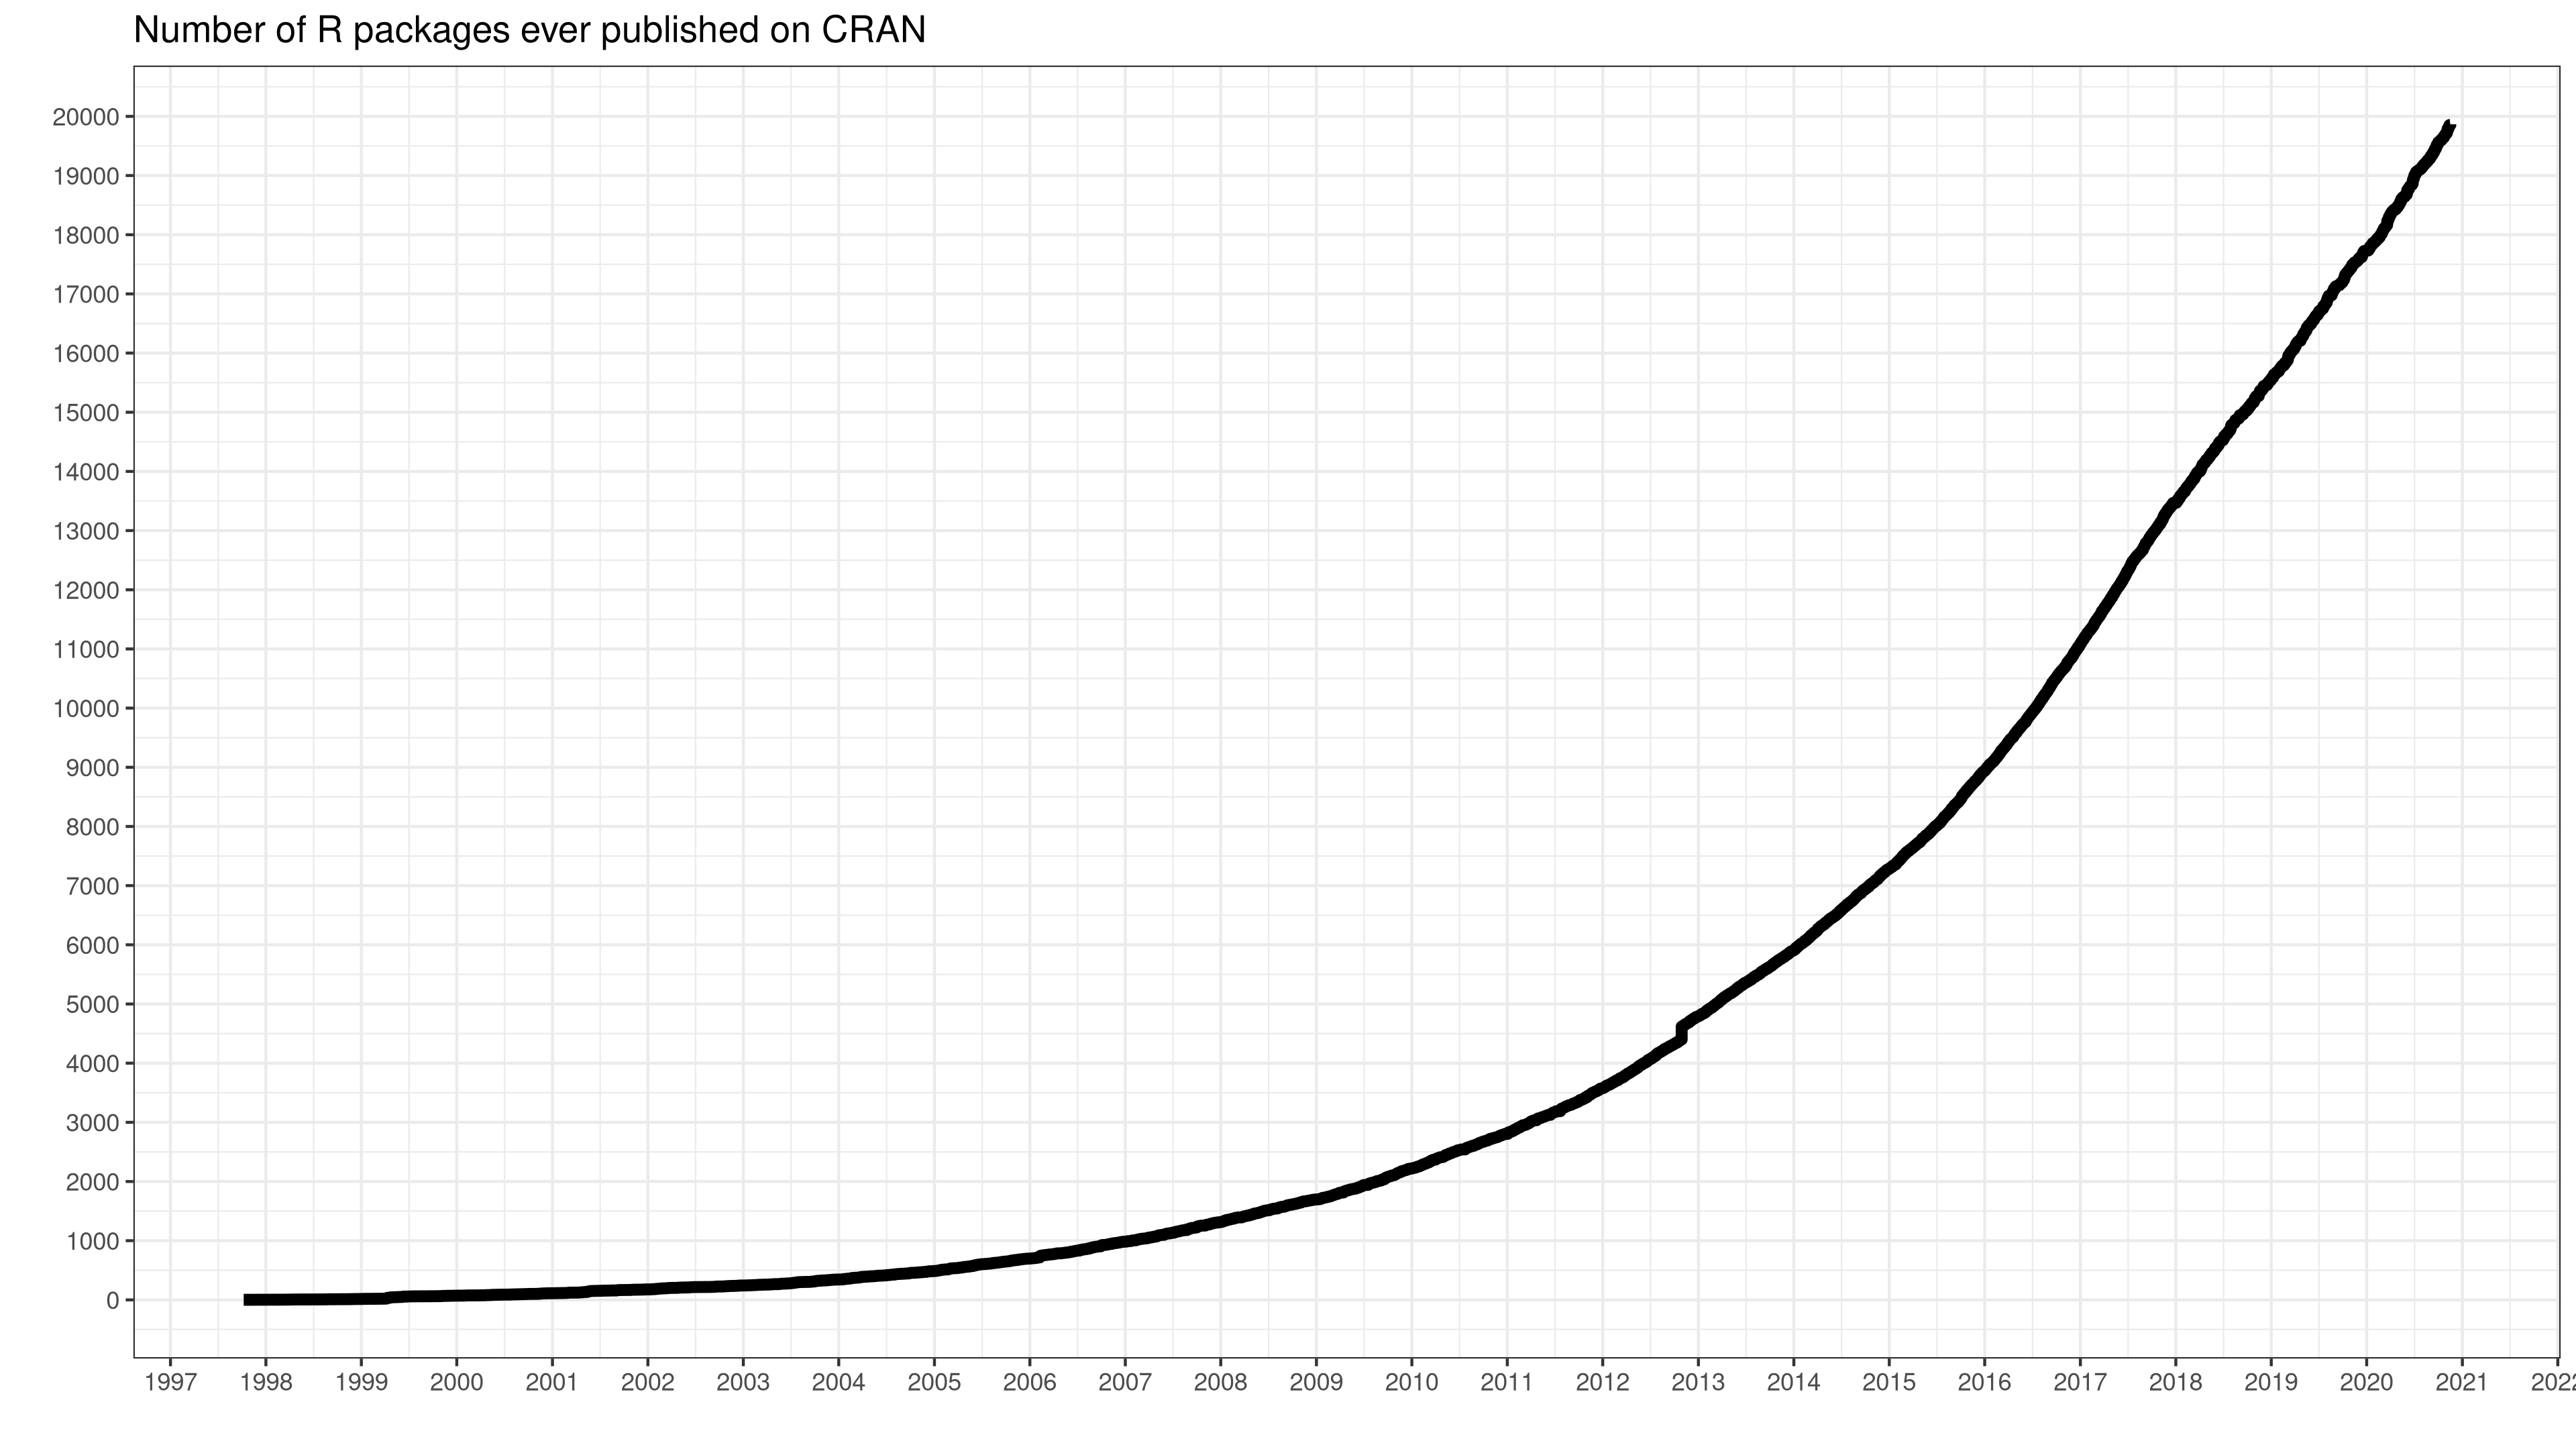
\includegraphics{img/number-of-submitted-packages-to-CRAN.png}

}

\caption{\label{fig-cran}Die Anzahl der R-Pakete ist exponenziell
gewachsen}

\end{figure}%

\subsection{Pakete installieren}\label{sec-install-r-pckgs}

Wie jede Software muss man Pakete (Erweiterungen für R) erst einmal
installieren, bevor man sie verwenden kann. Ja, einmal installieren
reicht.

Das geht komfortabel, wenn man beim Reiter \emph{Packages} auf
\emph{Install} klickt (s. Abbildung~\ref{fig-pckgs}) und dann den Namen
des zu installierenden Pakets eingibt.

\begin{figure}

\begin{minipage}{0.40\linewidth}

\centering{

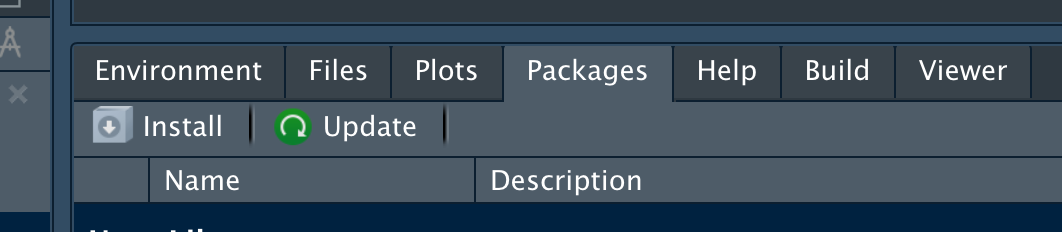
\includegraphics{img/install-packages.png}

}

\subcaption{\label{fig-install-packages}Klicken Sie auf ``Install'' im
Reiter ``Packages'', um R-Pakete zu installieren}

\end{minipage}%
%
\begin{minipage}{0.20\linewidth}
\end{minipage}%
%
\begin{minipage}{0.40\linewidth}

\centering{

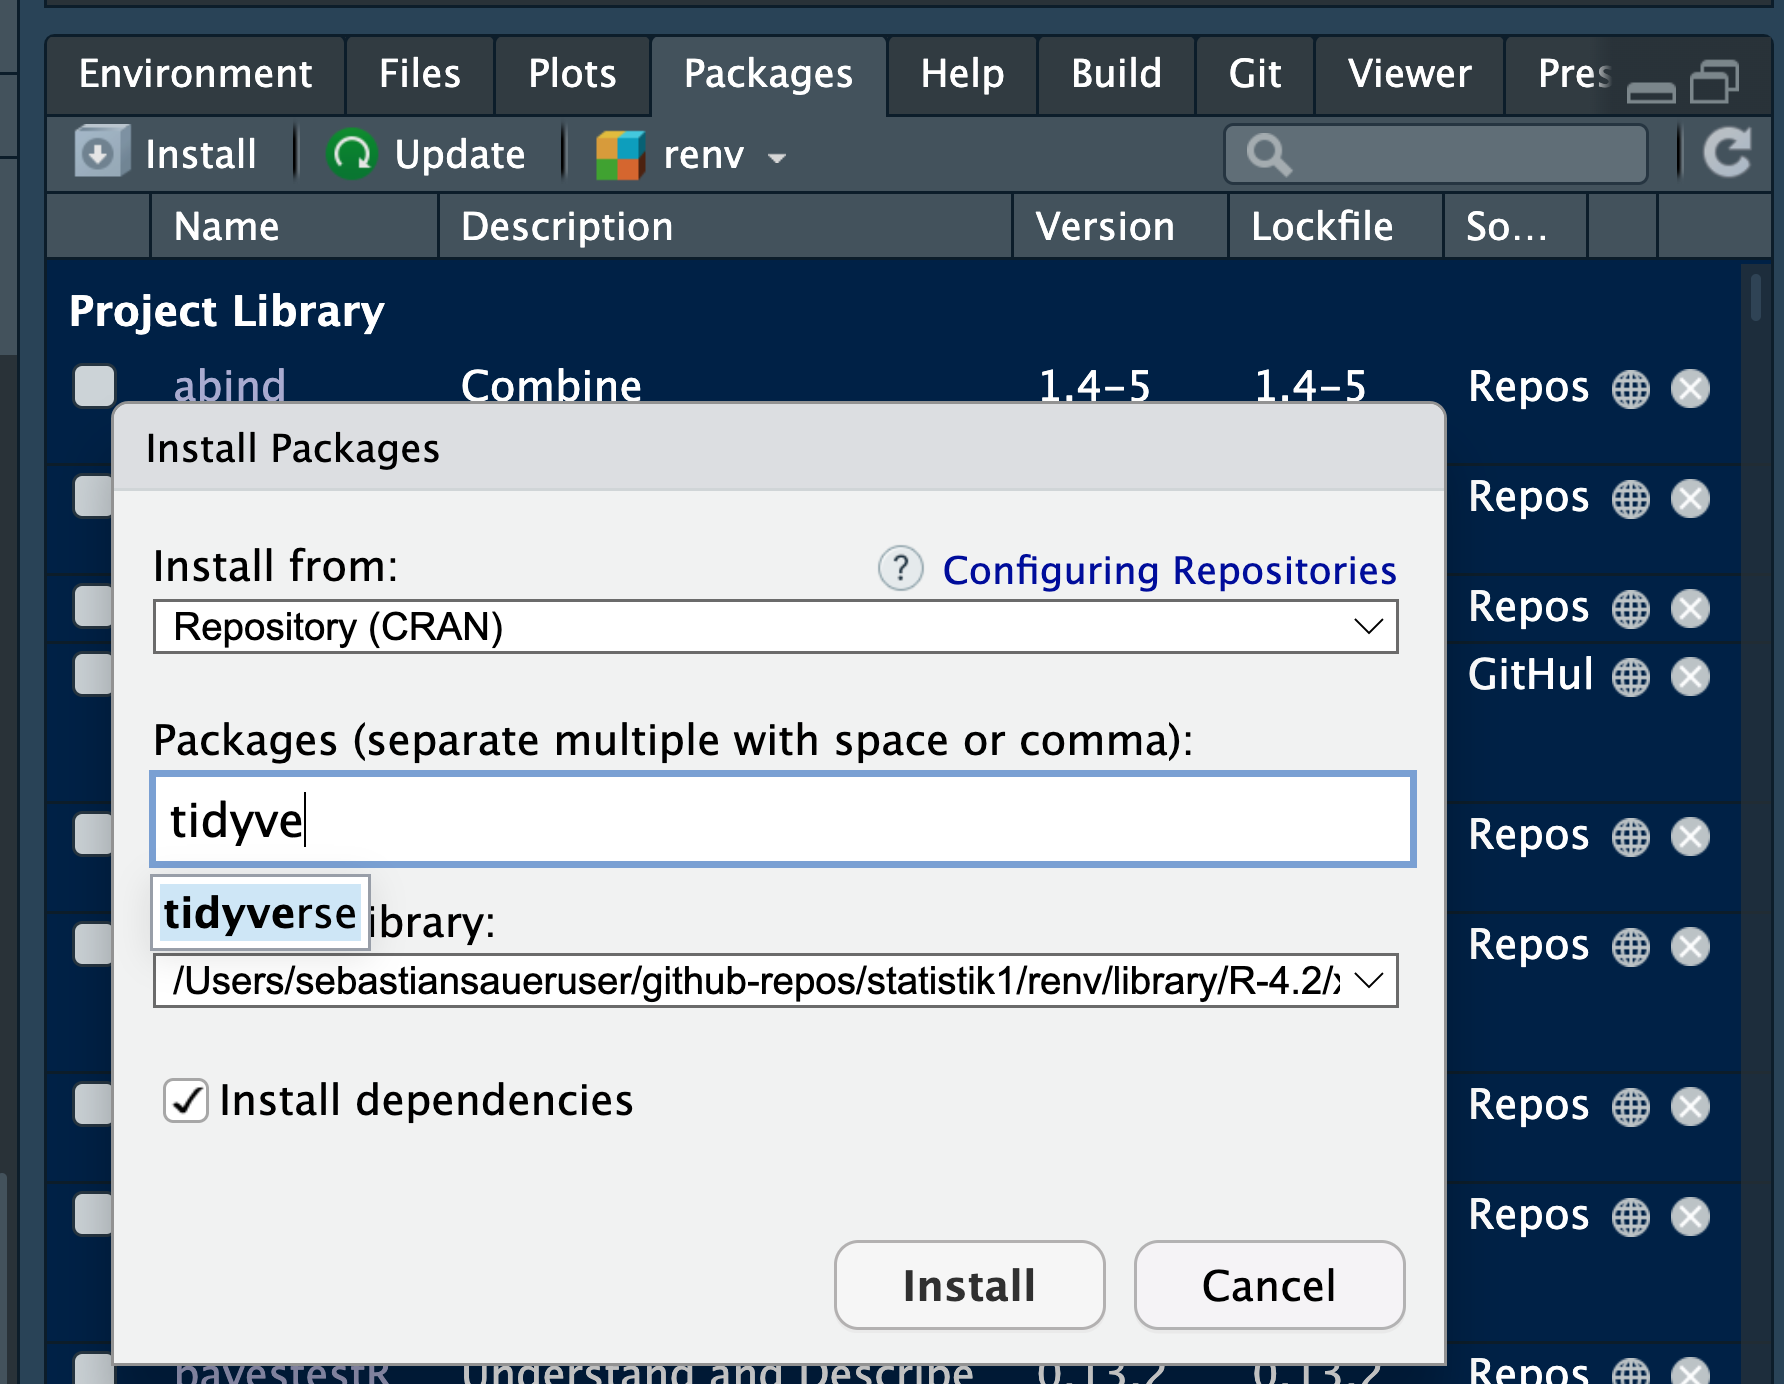
\includegraphics{img/install-packages3.png}

}

\subcaption{\label{fig-so-installieren}Geben Sie den Namen des zu
installierenden R-Pakets in dieser Maske ein}

\end{minipage}%

\end{figure}%

\begin{quote}
{\emoji{student}} Welche R-Pakete sind denn schon installiert?
\end{quote}

Im Reiter \emph{Packages} können Sie nachschauen, welche Pakete auf
Ihrem Computer schon installiert sind. Diese Pakete brauchen Sie
logischerweise dann \emph{nicht} noch mal installieren, s.
Abbildung~\ref{fig-paket-installiert}; es sei denn, Sie wollen das Paket
updaten.

\begin{figure}

\centering{

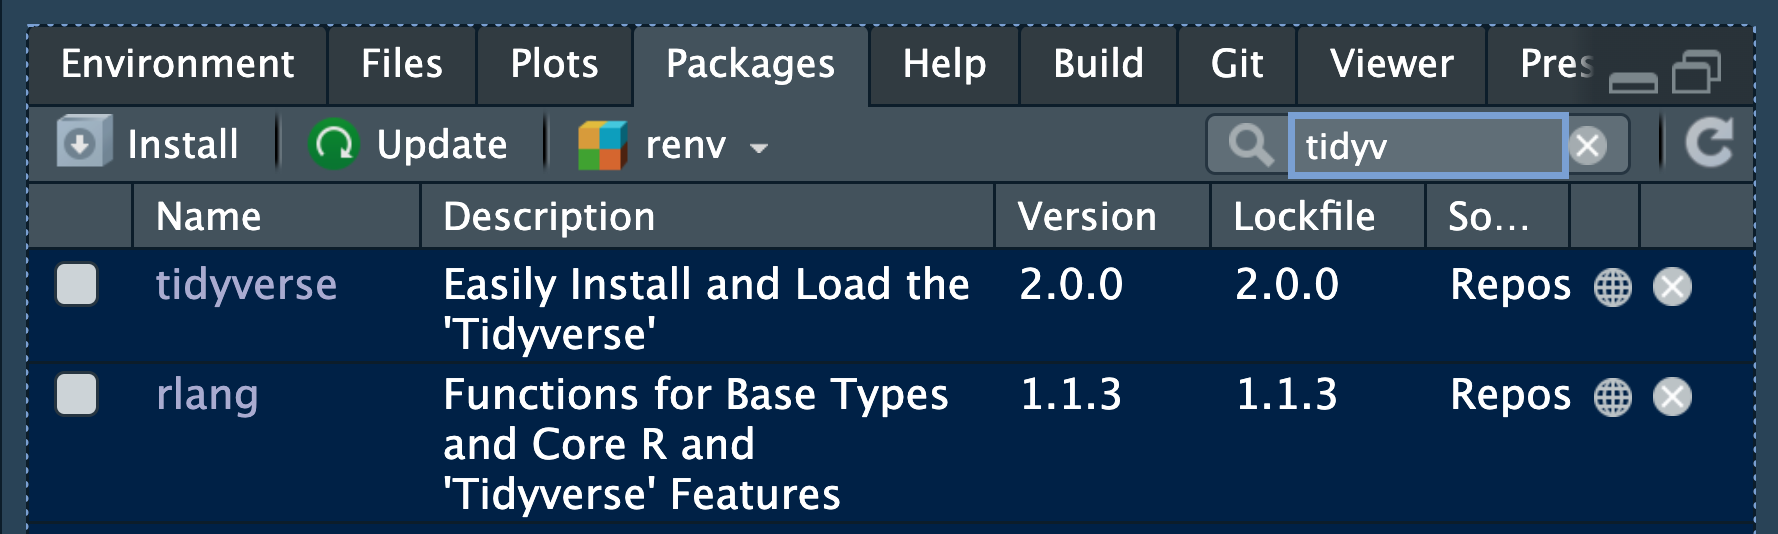
\includegraphics{img/paket-installiert.png}

}

\caption{\label{fig-paket-installiert}So sehen Sie, ob ein R-Paket auf
Ihrem System installiert ist}

\end{figure}%

Alternativ können Sie zum Installieren von Paketen auch den Befehl
\texttt{install.packages()} verwenden. Also zum Beispiel
\texttt{install.packages(tidyverse)} um das Paket \texttt{tidyverse} zu
installieren.

\begin{quote}
{\emoji{student}} Ja, aber welche R-Pakete ``soll'' ich denn
installieren, welche brauch ich denn?
\end{quote}

Im Moment sollten Sie die folgenden Pakete installiert haben:

\begin{itemize}
\tightlist
\item
  \texttt{tidyverse}
\item
  \texttt{easystats}
\end{itemize}

Wenn Sie die noch nicht installiert haben sollten, dann können Sie das
jetzt ja nachholen. (Übrigens sind \texttt{tidyverse} und
\texttt{easystats} Pakete, die nur dafür da sind, mehrere Pakete zu
installieren. So gehören z.B. zu \texttt{tidyverse} die Pakete
\texttt{ggplot} (Daten verbildlichen) und \texttt{dplyr} (Datenjudo).
Damit wir nicht alle Pakete einzeln installieren und starten müssen,
bietet uns das Paket \texttt{tidyverse} den Komfort, alle die Pakete
dieser ``Sammlung'' auf einmal zu starten. Praktisch.)

\begin{tcolorbox}[enhanced jigsaw, titlerule=0mm, left=2mm, toprule=.15mm, opacitybacktitle=0.6, breakable, bottomrule=.15mm, coltitle=black, colframe=quarto-callout-caution-color-frame, bottomtitle=1mm, title=\textcolor{quarto-callout-caution-color}{\faFire}\hspace{0.5em}{Vorsicht}, opacityback=0, arc=.35mm, toptitle=1mm, colbacktitle=quarto-callout-caution-color!10!white, rightrule=.15mm, leftrule=.75mm, colback=white]

Bevor Sie ein R-Paket (oder überhaupt irgendwelche Software)
installieren/updaten, sollten Sie das R-Paket schließen/beenden. Sonst
schrauben Sie an einem elektrischen Gerät herum, das noch unter Strom
steht (nicht gut). Die einfachste Art, alle Pakete zu beenden ist,
\texttt{Session\ \textgreater{}\ Restart\ R} zu klicken (in
RStudio).\(\square\)

\end{tcolorbox}

\subsection{Pakete starten}\label{pakete-starten}

Wenn Sie ein Softwareprogramm -- nichts anderes sind R-Pakete --
installiert haben, müssen Sie es noch \emph{starten}. Sie erkennen
leicht, ob ein Paket gestartet ist, wenn Sie ein Häkchen vor dem Namen
des Pakets in der Paketliste (Reiter \emph{Packages}) sehen, s.
Abbildung Abbildung~\ref{fig-install-packages}.\footnote{Dieses Video
  \url{https://www.youtube.com/watch?v=Yej9xzKQ3yI&list=PLRR4REmBgpIEaIyeNBgNGPgmhQJ_T1y8_&index=26}
  verdeutlicht den Unterschied zwischen \emph{Installation} und
  \emph{Starten} eines R-Pakets.}

\begin{tcolorbox}[enhanced jigsaw, titlerule=0mm, left=2mm, toprule=.15mm, opacitybacktitle=0.6, breakable, bottomrule=.15mm, coltitle=black, colframe=quarto-callout-note-color-frame, bottomtitle=1mm, title=\textcolor{quarto-callout-note-color}{\faInfo}\hspace{0.5em}{Hinweis}, opacityback=0, arc=.35mm, toptitle=1mm, colbacktitle=quarto-callout-note-color!10!white, rightrule=.15mm, leftrule=.75mm, colback=white]

Ein bestimmtes R-Paket muss man nur \emph{einmalig installieren}. Aber
man muss es \emph{jedes Mal neu starten}, wenn man R (bzw. RStudio)
startet. \(\square\)

\end{tcolorbox}

\section{Mit R arbeiten}\label{mit-r-arbeiten}

\subsection{Projekte in R}\label{projekte-in-r}

Ein \emph{Projekt} in RStudio (s. Abbildung~\ref{fig-projects}) ist
letztlich ein Ordner, der als ``Basis'' für eine Reihe von Dateien
verwendet wird. Sagen wir, Sie nennen Ihr Projekt \texttt{cool\_stuff}.
RStudio legt uns diesen Ordner an einem von uns gewählten Platz auf
unserem Computer an. Das ist ganz praktisch, weil man dann sagen kann
``Hey R, nimmt die Datei `daten.csv'\,'', ohne einen Pfad anzugeben.
Vorausgesetzt, die Datei liegt auch im Projektordner
(\texttt{cool\_stuff}).

Projekte kann anlegen mit Klick auf das Icon, das einen Quader mit dem
Buchstaben R darin anzeigt (s. Abbildung~\ref{fig-rstudio-projekte}).
RStudio-Projekte machen Ihr Leben leichter (s.
Abbildung~\ref{fig-projects}).

Nutzen Sie RStudio-Projekte, das macht Ihr Leben leichter.

\begin{figure}

\centering{

\begin{figure}[H]

\begin{minipage}{0.80\linewidth}

\centering{

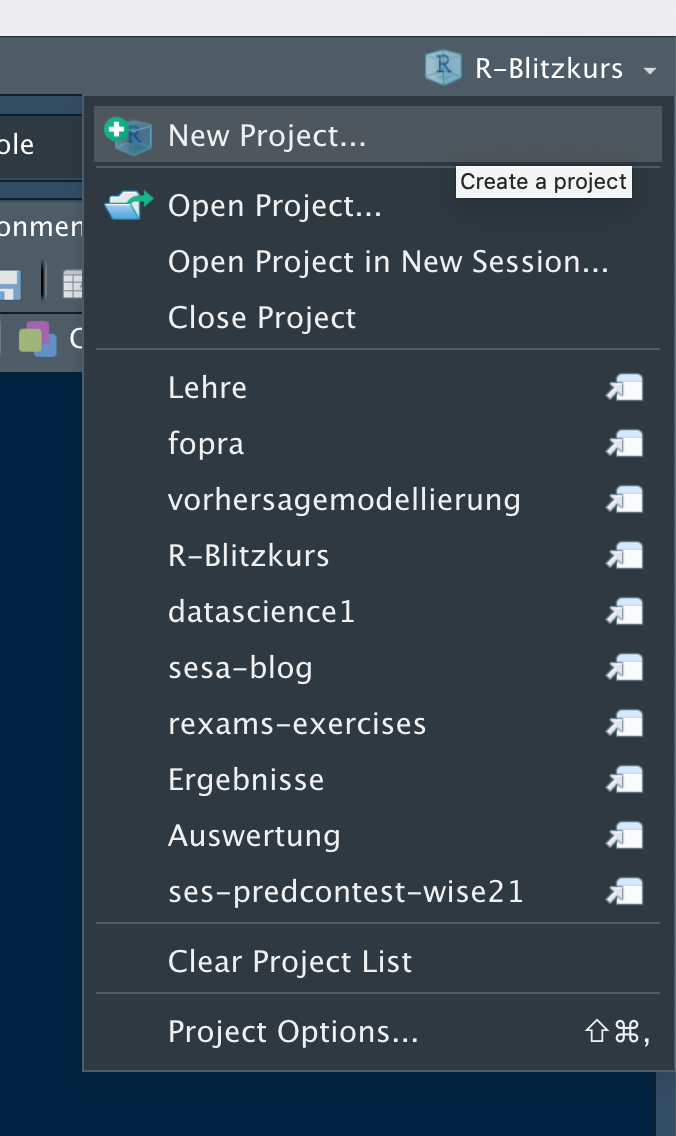
\includegraphics[width=0.5\textwidth,height=\textheight]{img/rstudio-projekte.png}

}

\subcaption{\label{fig-rstudio-projekte}RStudio-Projekte, Beispiele}

\end{minipage}%
%
\begin{minipage}{0.20\linewidth}

\centering{

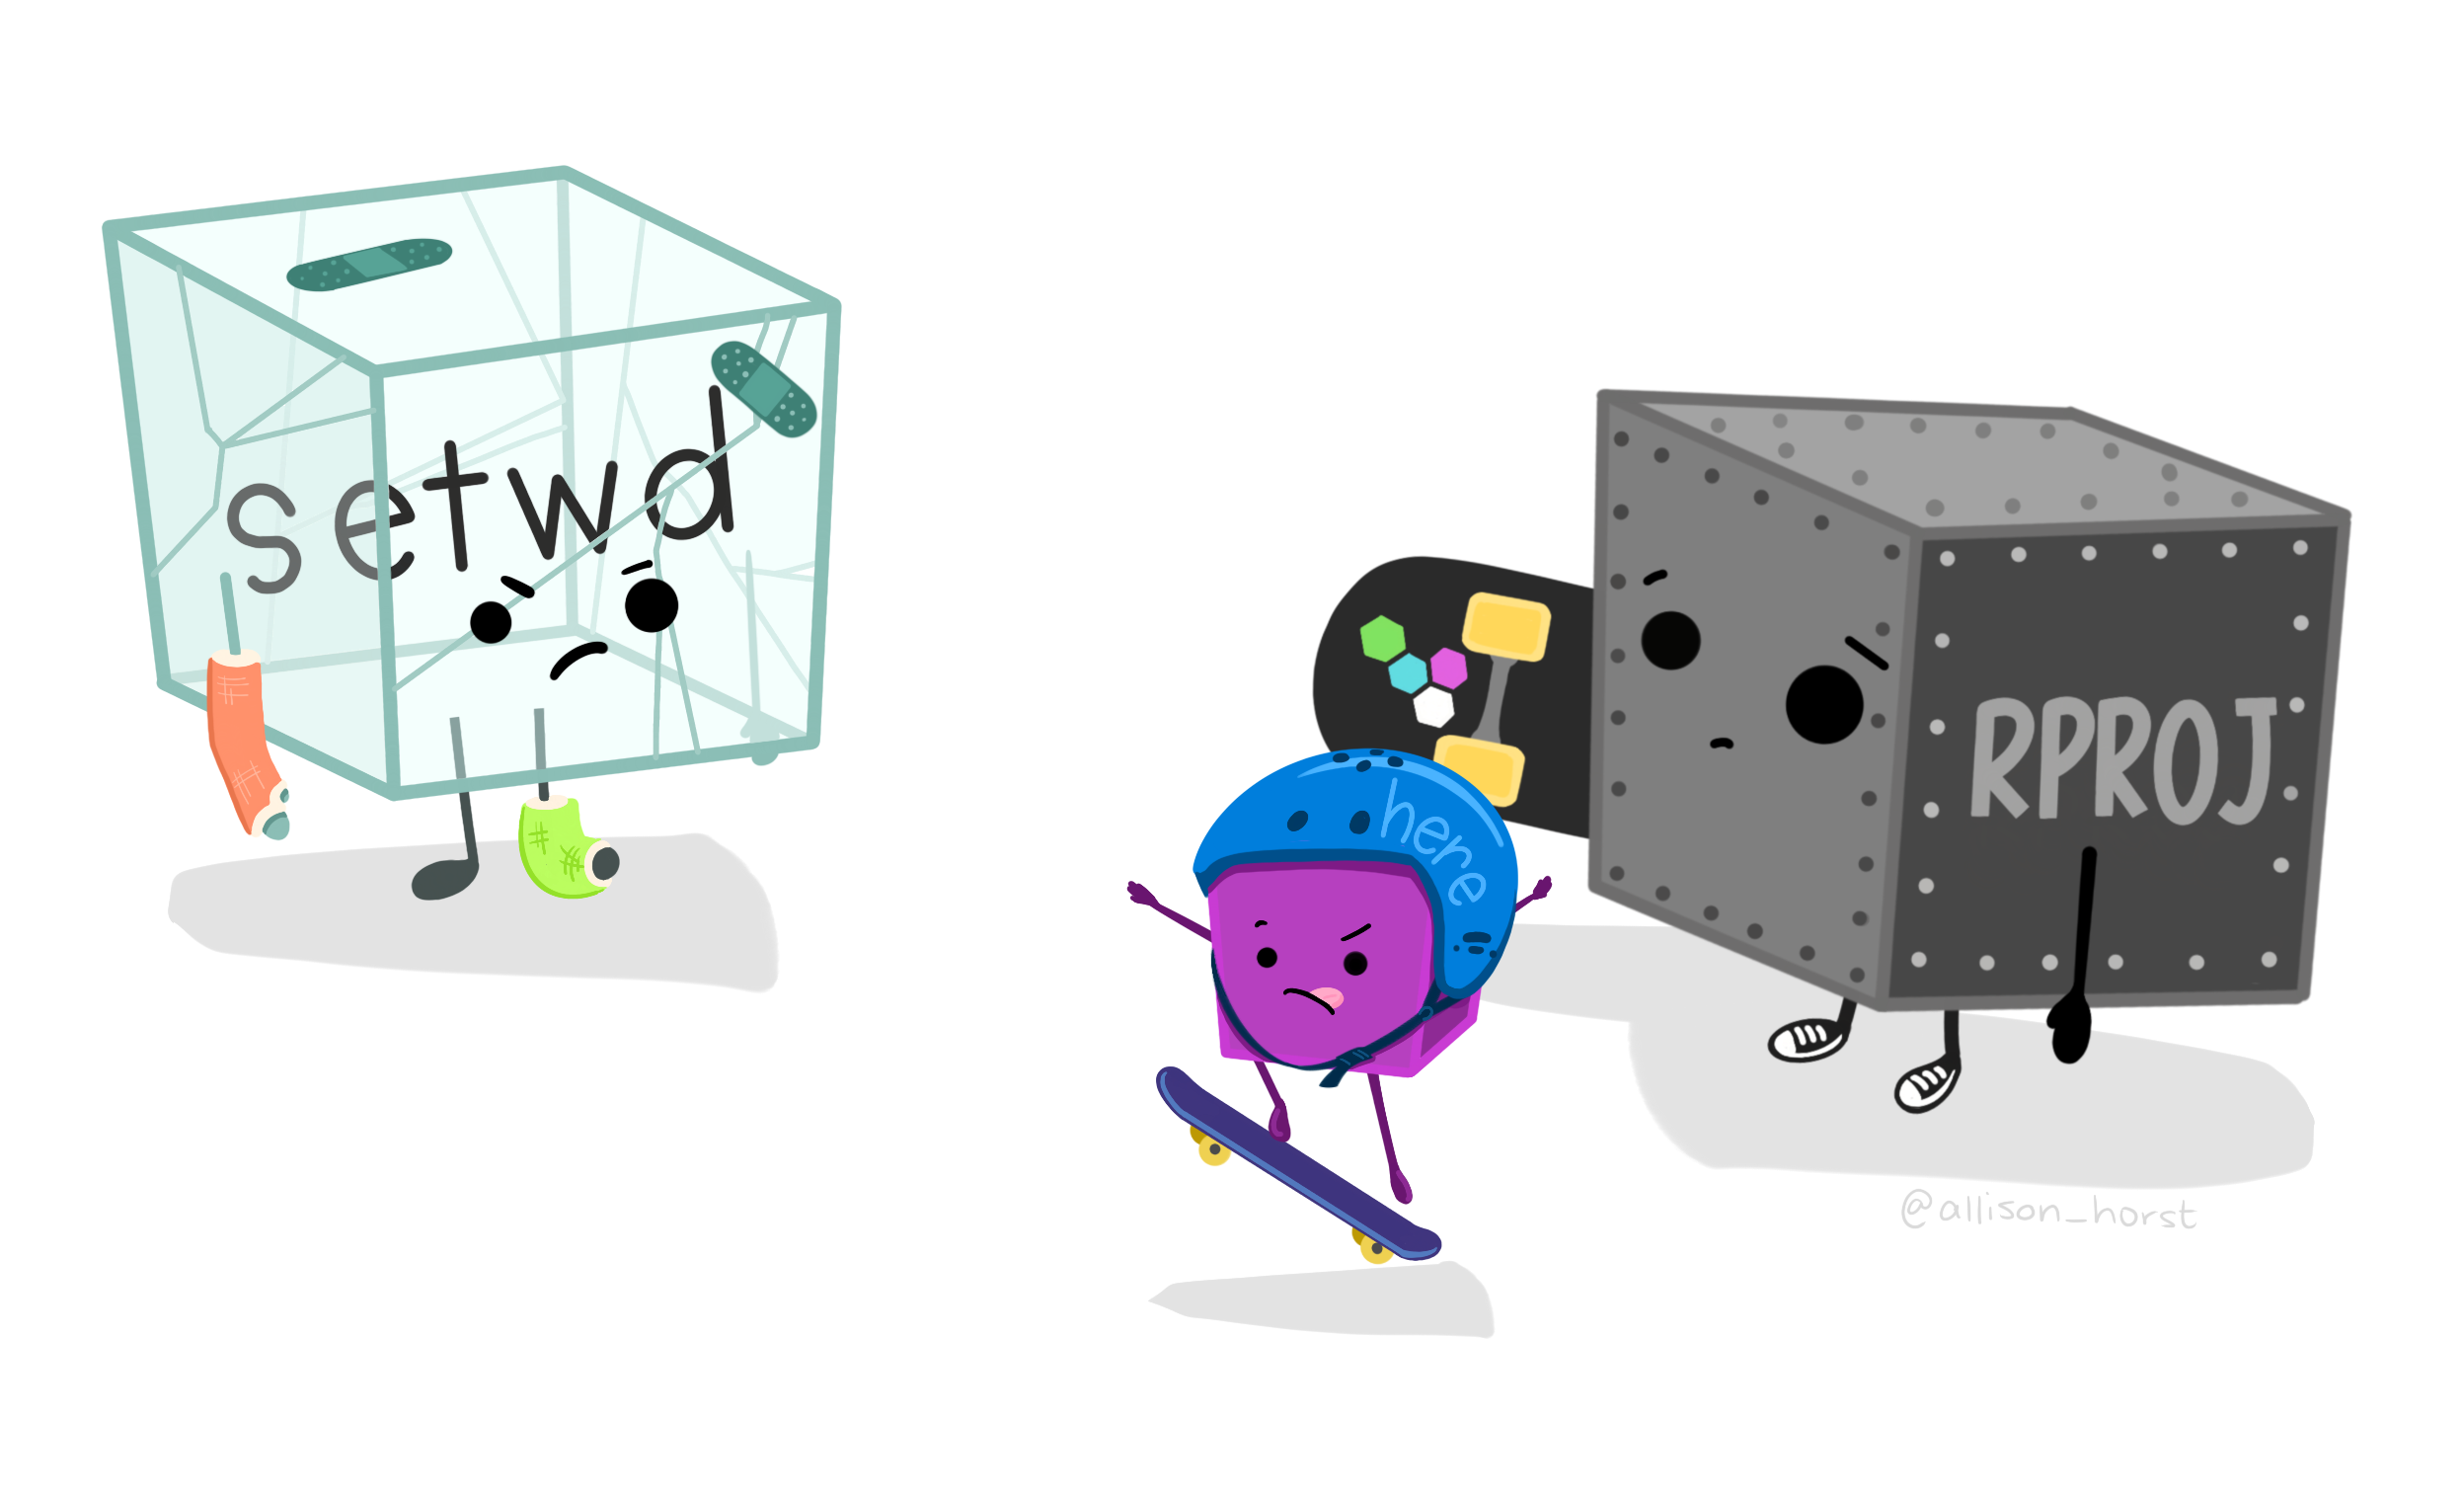
\includegraphics{img/cracked_setwd.png}

}

\subcaption{\label{fig-setwd}RStudio-Projekte sind viel sicherer als das
Arbeitsverzeichnis von Hand zu wählen oder mit Pfaden herumzubasteln
(Horst, 2024)}

\end{minipage}%

\end{figure}%

}

\caption{\label{fig-projects}}

\end{figure}%

\subsection{Skriptdateien}\label{skriptdateien}

Die R-Befehle (``Syntax'') schreiben Sie am besten in eine speziell
dafür vorgesehene Textdatei in RStudio. Eine Sammlung von
(R-)Computer-Befehlen nennt man auch ein \emph{Skript}, daher spricht
man auch von einer \emph{Skriptdatei}.

\subsubsection{So erstellen Sie eine neue
Skriptdatei}\label{so-erstellen-sie-eine-neue-skriptdatei}

Um eine neue R-Skriptdatei zu erstellen, klicken Sie auf das Icon, das
ein weißes Blatt mit einem grünen Pluszeichen zeigt, s.
Abbildung~\ref{fig-script-new}.

\begin{figure}

\begin{minipage}{0.50\linewidth}

\centering{

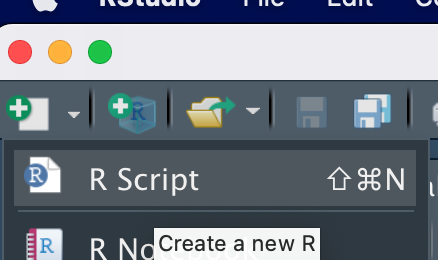
\includegraphics[width=0.5\textwidth,height=\textheight]{img/script-new.png}

}

\subcaption{\label{fig-script-new1}So erstellen Sie eine neue
Skriptdatei}

\end{minipage}%
%
\begin{minipage}{0.50\linewidth}

\centering{

\includegraphics{img/neue-skriptdatei.png}

}

\subcaption{\label{fig-script-new2}Klicken Sie auf das Icon mit dem
leeren Blatt und dem grünen Plus}

\end{minipage}%

\caption{\label{fig-script-new}Es gibt verschiedene Wege, um eine neue
R-Skript-Datei in RStudio zu öffnen.}

\end{figure}%

\subsubsection{So speichern Sie Ihre
Skripdatei}\label{so-speichern-sie-ihre-skripdatei}

Vergessen Sie nicht zu \emph{speichern}, wenn Sie ein tolles Skript
geschrieben haben. Dafür gibt es mehrere Möglichkeiten:

\begin{enumerate}
\def\labelenumi{\arabic{enumi}.}
\tightlist
\item
  Tastaturkürzel \emph{Strg+S}
\item
  Menü: \texttt{File\ \textgreater{}\ Save}
\item
  Klick auf das Icon mit der Diskette, s.
  Abbildung~\ref{fig-script-new}.
\end{enumerate}

\subsubsection{So öffnen Sie eine
Skriptdatei}\label{so-uxf6ffnen-sie-eine-skriptdatei}

Eine existierende Skriptdatei können Sie in typischer Manier
\emph{öffnen}:

\begin{enumerate}
\def\labelenumi{\arabic{enumi}.}
\tightlist
\item
  Strg+O
\item
  Klick auf das Icon mit der Akte und dem grünen Pfeil (vgl.
  Abbildung~\ref{fig-script-new})
\item
  Menü: \texttt{File\ \textgreater{}\ Open\ File...}
\end{enumerate}

\subsection{Quarto-Dokumente}\label{quarto-dokumente}

\href{https://quarto.org/}{Quarto}\footnote{\url{https://quarto.org/}}
ist ein Programm zum Erstellen von Texten, in die man R-Syntax einfügen
kann. Die Ausgaben der R-Befehle werden dann direkt im Dokument
eingebunden. Abbildung~\ref{fig-exm-quarto} zeit ein Beispiel für ein
Quarto-Dokument.

\begin{tcolorbox}[enhanced jigsaw, titlerule=0mm, left=2mm, toprule=.15mm, opacitybacktitle=0.6, breakable, bottomrule=.15mm, coltitle=black, colframe=quarto-callout-note-color-frame, bottomtitle=1mm, title=\textcolor{quarto-callout-note-color}{\faInfo}\hspace{0.5em}{Hinweis}, opacityback=0, arc=.35mm, toptitle=1mm, colbacktitle=quarto-callout-note-color!10!white, rightrule=.15mm, leftrule=.75mm, colback=white]

Quarto ist eine komfortable und leistungsfähige Methode, um Dokumente
mit R-Syntax zu schreiben. Sie sind aber nicht verpflichtet, Quarto zu
nutzen. Stattdessen können Sie Ihre Syntax auch in Skriptdateien
schreiben. \(\square\)

\end{tcolorbox}

\begin{figure}

\centering{

\includegraphics{index_files/mediabag/rstudio-hello.png}

}

\caption{\label{fig-exm-quarto}Dokumente schreiben mit Quarto}

\end{figure}%

Wenn Sie Quarto nutzen möchten, müssen Sie es zunächst installieren,
d.h. \href{https://quarto.org/docs/get-started/}{herunterladen}. Dann
können Sie in RStudio Quarto-Dateien erstellen.\footnote{\url{https://quarto.org/docs/get-started/}}
Ein neues Quarto-Dokument können Sie erstellen mit Klick auf \emph{File
\textgreater{} New File \textgreater{} Quarto Document
\ldots{}}.\footnote{Dieses Video \url{https://youtu.be/_f3latmOhew} gibt
  Ihnen Einstiegshilfe in Quarto.}

\section{Errisch für Einsteiger}\label{errisch-fuxfcr-einsteiger}

\begin{tcolorbox}[enhanced jigsaw, titlerule=0mm, left=2mm, toprule=.15mm, opacitybacktitle=0.6, breakable, bottomrule=.15mm, coltitle=black, colframe=quarto-callout-note-color-frame, bottomtitle=1mm, title=\textcolor{quarto-callout-note-color}{\faInfo}\hspace{0.5em}{Hinweis}, opacityback=0, arc=.35mm, toptitle=1mm, colbacktitle=quarto-callout-note-color!10!white, rightrule=.15mm, leftrule=.75mm, colback=white]

Sie finden den R-Code für jedes Kapitel
\href{https://github.com/sebastiansauer/statistik1/tree/main/R-code-for-all-chapters}{hier}:
\url{https://github.com/sebastiansauer/statistik1/tree/main/R-code-for-all-chapters}.
\(\square\)

\end{tcolorbox}

\subsection{Variablen}\label{sec-rvars}

In jeder Programmiersprache kann man Variablen definieren, so auch in R:

\begin{Shaded}
\begin{Highlighting}[]
\NormalTok{richtige\_antwort }\OtherTok{=} \DecValTok{42}
\NormalTok{falsche\_antwort }\OtherTok{=} \DecValTok{43}
\NormalTok{typ }\OtherTok{=} \StringTok{"Antwort"}
\NormalTok{ist\_korrekt }\OtherTok{=} \ConstantTok{TRUE}
\end{Highlighting}
\end{Shaded}

Alternativ zum Gleichheitszeichen \texttt{=} können Sie auch (synonym)
den Zuweisungspfeil \texttt{\textless{}-} verwenden. Beides führt zum
gleichen Ergebnis. Allerdings ist der Zuweisungspfeil präziser, und
sollte daher \emph{bevorzugt} werden.

Der \emph{Zuweisungspfeil} \texttt{\textless{}-} bzw. das
Gleichheitszeichen \texttt{=} definiert eine neue \emph{Variable} (oder
überschreibt den Inhalt, wenn die Variable schon existiert).\footnote{Dieses
  Video
  \url{https://www.youtube.com/watch?v=TKQk-tEF9YQ&list=PLRR4REmBgpIEaIyeNBgNGPgmhQJ_T1y8_&index=28}
  und dieses Video
  \url{https://www.youtube.com/watch?v=Nal0m_AmMwg&list=PLRR4REmBgpIEaIyeNBgNGPgmhQJ_T1y8_&index=48}
  geben eine Einführung in das Definieren von Variablen in R}

\begin{Shaded}
\begin{Highlighting}[]
\NormalTok{richtige\_antwort }\OtherTok{\textless{}{-}} \DecValTok{42}
\NormalTok{falsche\_antwort }\OtherTok{\textless{}{-}} \DecValTok{43}
\NormalTok{typ }\OtherTok{\textless{}{-}} \StringTok{"Antwort"}
\NormalTok{ist\_korrekt }\OtherTok{\textless{}{-}} \ConstantTok{TRUE}
\end{Highlighting}
\end{Shaded}

Sie können sich eine Variable wie einen Becher oder Behälter vorstellen,
der bestimmte Werte enthält. Auf dem Becher steht (mit Edding
geschrieben) der Name des Bechers. Natürlich können Sie die Werte aus
dem Becher entfernen und sie durch neue ersetzen (vgl.
Abbildung~\ref{fig-def-vars}).

\begin{figure}

\centering{

\includegraphics[width=0.25\textwidth,height=\textheight]{img/Variablen_zuweisen.png}

}

\caption{\label{fig-def-vars}Variablen zuweisen}

\end{figure}%

R kann übrigens auch rechnen. Probieren Sie es doch gleich mal hier aus!

\begin{Shaded}
\begin{Highlighting}[]
\NormalTok{die\_summe }\OtherTok{\textless{}{-}}\NormalTok{ falsche\_antwort }\SpecialCharTok{+}\NormalTok{ richtige\_antwort}
\end{Highlighting}
\end{Shaded}

Aber was ist jetzt der Wert, der ``Inhalt'' der Variable
\texttt{die\_summe}?

Um den Wert, d.h. den Inhalt einer Variablen in R \emph{auszulesen},
geben wir einfach den Namen des Objekts ein:

\begin{Shaded}
\begin{Highlighting}[]
\NormalTok{die\_summe}
\DocumentationTok{\#\# [1] 85}
\end{Highlighting}
\end{Shaded}

Was passiert wohl, wenn wir \texttt{die\_summe} jetzt wie folgt
definieren?

\begin{Shaded}
\begin{Highlighting}[]
\NormalTok{die\_summe }\OtherTok{\textless{}{-}}\NormalTok{ falsche\_antwort }\SpecialCharTok{+}\NormalTok{ richtige\_antwort }\SpecialCharTok{+} \DecValTok{1}
\end{Highlighting}
\end{Shaded}

Wer hätt's geahnt:

\begin{Shaded}
\begin{Highlighting}[]
\NormalTok{die\_summe}
\DocumentationTok{\#\# [1] 86}
\end{Highlighting}
\end{Shaded}

Variablen können auch ``leer'' sein:

\begin{Shaded}
\begin{Highlighting}[]
\NormalTok{alter }\OtherTok{\textless{}{-}} \ConstantTok{NA}
\NormalTok{alter}
\DocumentationTok{\#\# [1] NA}
\end{Highlighting}
\end{Shaded}

\texttt{NA} steht für \emph{not available}, nicht verfügbar und macht
deutlich, dass hier ein Wert fehlt.

\begin{quote}
{\emoji{student}} Wozu brauche ich bitte fehlende Werte?!
\end{quote}

Fehlende Werte sind ein häufiges Problem in der Praxis. Vielleicht hat
sich die befragte Person geweigert, ihr Alter anzugeben (Datenschutz!).
Oder als Sie die Daten in Ihren Computer eingeben wollten, ist Ihre
Katze über die Tastatur gelaufen und alles war futsch\ldots{}

\subsection{Funktionen (``Befehle'')}\label{funktionen-befehle}

Das, was R kann, ist in ``Funktionen'' hinterlegt. Genauer gesagt ist
ein ``Befehl'' eine Funktion.

\begin{definition}[Funktion]\protect\hypertarget{def-fun}{}\label{def-fun}

Eine Funktion ist eine Regel, die jedem Eingabewert (auch Argument
genannt) einen Ausgabewert zuordnet. Man kann sich Funktionen als
Maschinen vorstellen, die Eingabedaten in Ausgabedaten umwandeln, vgl.
Abbildung~\ref{fig-function-schema}. \(\square\)

\end{definition}

\subsubsection{Eine erste Funktion: Vektoren
erstellen}\label{eine-erste-funktion-vektoren-erstellen}

Ein Beispiel für eine solche Funktion könnte sein: ``Berechne den
Mittelwert dieser Datenreihe'' (schauen wir uns gleich an).

Das geht so:

\begin{Shaded}
\begin{Highlighting}[]
\NormalTok{Antworten }\OtherTok{\textless{}{-}} \FunctionTok{c}\NormalTok{(}\DecValTok{42}\NormalTok{, }\DecValTok{43}\NormalTok{)}
\end{Highlighting}
\end{Shaded}

Der Befehl \texttt{c} (c wie \emph{c}ombine) fügt mehrere Werte zusammen
zu einer ``Liste'' (einem Vektor). (Streng genommen sollte man nicht von
einer Liste sprechen, da es in R noch einen anderen Objekttyp gibt, der
\texttt{list} heißt, und eine verallgemeinerte Form eines Vektors ist.)

\begin{definition}[Vektor]\protect\hypertarget{def-vektor}{}\label{def-vektor}

Als \emph{Vektor} (Datenreihe) bezeichnen wir eine geordnete Folge von
Werten. In R kann man sie mit der Funktion \texttt{c()} erstellen. Die
Werte eines Vektors bezeichnet man als \emph{Elemente}. \(\square\)

\end{definition}

Mit dem Zuweisungspfeil geben wir diesem Vektor einen Namen, hier
\texttt{Antworten}. Dieser Vektor besteht aus zwei Werten, zuerst
\texttt{42}, dann kommt \texttt{43}.

\begin{example}[Beispiele für
Vektoren]\protect\hypertarget{exm-vektoren}{}\label{exm-vektoren}

Vektoren können (praktisch) beliebig lang sein, z.B. drei Elemente.

\begin{Shaded}
\begin{Highlighting}[]
\NormalTok{x }\OtherTok{\textless{}{-}} \FunctionTok{c}\NormalTok{(}\DecValTok{1}\NormalTok{, }\DecValTok{2}\NormalTok{, }\DecValTok{3}\NormalTok{)}
\NormalTok{y }\OtherTok{\textless{}{-}} \FunctionTok{c}\NormalTok{(}\DecValTok{2}\NormalTok{, }\DecValTok{1}\NormalTok{, }\DecValTok{3}\NormalTok{)  }\CommentTok{\# x und y sind ungleich (Reihenfolge der Werte)}
\NormalTok{z }\OtherTok{\textless{}{-}} \FunctionTok{c}\NormalTok{(}\FloatTok{3.14}\NormalTok{, }\FloatTok{2.71}\NormalTok{)  }
\NormalTok{namen }\OtherTok{\textless{}{-}} \FunctionTok{c}\NormalTok{(}\StringTok{"Anni"}\NormalTok{, }\StringTok{"Bert"}\NormalTok{, }\StringTok{"Charli"}\NormalTok{) }\CommentTok{\# Text{-}Vektor}
\end{Highlighting}
\end{Shaded}

\end{example}

Zwei wichtige Typen von Vektoren sind numerische Vektoren (reelle
Zahlen; in R auch als \emph{numeric} oder \emph{double} bezeichnet) und
Textvektoren, in R auch als \emph{String} oder \emph{character}
bezeichnet.

\begin{example}[]\protect\hypertarget{exm-funs}{}\label{exm-funs}

Weitere Beispiel für Funktionen sind:

\begin{itemize}
\tightlist
\item
  ``Erstelle eine Liste (Vektor) von Werten''.
\item
  ``Lade dieses R-Paket.''
\item
  ``Gib den größten Wert dieser Datenreihe aus.'' \(\square\)
\end{itemize}

\end{example}

\subsection{Unsere erste statistische Funktion}\label{sec-first-fun}

Jetzt wird's ernst. Jetzt kommt die Statistik. Berechnen wir also unsere
erste statistische Funktion: Den Mittelwert. Puh.

\begin{Shaded}
\begin{Highlighting}[]
\FunctionTok{mean}\NormalTok{(Antworten)}
\DocumentationTok{\#\# [1] 42}
\end{Highlighting}
\end{Shaded}

Sie hätten \texttt{Antworten} auch durch \texttt{c(42,\ 43)} ersetzen
können, so haben Sie ja schließlich die Variable gerade definiert.

R arbeitet so einen ``verschachtelten'' Befehl \emph{von innen nach
außen} ab:

Start: \texttt{mean(Antworten)}

{\(\downarrow\)}

Schritt 1: \texttt{mean(c(42,\ 43))}

{\(\downarrow\)}

Schritt 2: \texttt{42.5}

Abbildung~\ref{fig-function-schema} stellt eine Funktion schematisch
dar.

\begin{figure}

\centering{

\includegraphics[width=0.5\textwidth,height=\textheight]{img/function-schema.pdf}

}

\caption{\label{fig-function-schema}Schema einer Funktion}

\end{figure}%

Eine Funktion hat einen oder mehrere \emph{Inputs} (s.
Abbildung~\ref{fig-function-schema}), das sind Daten oder
Verarbeitungshinweise, die man in die Funktion \texttt{fun}
\emph{eingibt}, bevor sie loslegt. Eine Funktion hat immer (genau) eine
\emph{Ausgabe} (Output), in der das Ergebnis einer Funktion ausgegeben
wird.

\begin{definition}[Argumente einer
Funktion]\protect\hypertarget{def-args}{}\label{def-args}

Die ``Trichter'' einer (R-)Funktion, in denen man die Eingaben
``einfüllt'', nennt man auch \emph{Argumente}.\(\square\)

\end{definition}

So hat die Funktion \texttt{mean()} z.B. folgende Argumente, s.
Listing~\ref{lst-mean}.

\begin{codelisting}

\caption{\label{lst-mean}Die Argumente der R-Funktion \texttt{mean}}

\centering{

\begin{Shaded}
\begin{Highlighting}[]
\FunctionTok{mean}\NormalTok{(x, }\AttributeTok{trim =} \DecValTok{0}\NormalTok{, }\AttributeTok{na.rm =} \ConstantTok{FALSE}\NormalTok{, ...)}
\end{Highlighting}
\end{Shaded}

}

\end{codelisting}%

\begin{itemize}
\tightlist
\item
  \texttt{x}: das ist der Vektor, für den der Mittelwert berechnet
  werden soll
\item
  \texttt{trim\ =\ 0}: Sollen die extremsten Werte von \texttt{x} lieber
  ``abgeschnitten'' werden, also nicht in die Berechnung des Mittelwerts
  einfließen?
\item
  \texttt{na.rm\ =\ FALSE}: Wie soll mit fehlenden Werten \texttt{NA}
  umgegangen werden? Im Standard liefert \texttt{mean} (und viele andere
  arithmetische Funktionen in R) \texttt{NA} zurück. R schwenkt
  sozusagen die rote Fahne, um zu signalisieren, Achtung, Mensch, hier
  ist irgendwas nicht in Ordnung. Setzt man aber
  \texttt{na.rm\ =\ TRUE}, dann entfernt (remove, rm) R die fehlenden
  Werte und berechnet den Mittelwert, ohne weitere Hinweise zu den
  fehlenden Werten.
\item
  \texttt{...} heißt ``sonstiges Zeugs, das manchmal eine Rolle spielen
  könnte''; darum kümmern wir uns jetzt nicht.
\end{itemize}

Einige Argumente haben einen \emph{Standardwert} bzw. eine
\emph{Voreinstellung} (engl. \emph{default}). So wird bei der Funktion
\texttt{mean} im Standard nicht getrimmt (\texttt{trim\ =\ 0}) und
fehlende Werte werden nicht entfernt (\texttt{na.rm\ =\ FALSE)}.

\begin{tcolorbox}[enhanced jigsaw, titlerule=0mm, left=2mm, toprule=.15mm, opacitybacktitle=0.6, breakable, bottomrule=.15mm, coltitle=black, colframe=quarto-callout-note-color-frame, bottomtitle=1mm, title=\textcolor{quarto-callout-note-color}{\faInfo}\hspace{0.5em}{Hinweis}, opacityback=0, arc=.35mm, toptitle=1mm, colbacktitle=quarto-callout-note-color!10!white, rightrule=.15mm, leftrule=.75mm, colback=white]

Wenn ein R-Befehl ein Argument mit Voreinstellung hat, brauchen Sie
dieses Argument \emph{nicht} zu befüllen. In dem Fall wird auf den Wert
der Voreinstellung zurückgegriffen. Argumente ohne Voreinstellung -- wie
\texttt{x} bei \texttt{mean()} -- müssen Sie aber auf jeden Fall mit
einem Wert befüllen. Man würde also \texttt{mean} zumeist so aufrufen:
\texttt{mean(x)}. \(\square\)

\end{tcolorbox}

Bei jedem R-Befehl haben die Argumente eine bestimmte Reihenfolge, etwa
bei \texttt{mean()}:
\texttt{mean(x,\ trim\ =\ 0,\ na.rm\ =\ FALSE,\ ...)}.

(Nur) wenn man die Argumente in ihrer vorgegebenen Reihenfolge
anspricht, muss man \emph{nicht} den Namen des Arguments anführen:

\emoji{check-mark-button} \texttt{mean(Antworten,\ 0,\ FALSE)}

Hält man sich aber nicht an die vorgebene Reihenfolge, so weiß R nicht,
was zu tun ist und flüchtet sich in eine Fehlermeldung:

\begin{Shaded}
\begin{Highlighting}[]
\FunctionTok{mean}\NormalTok{(Antworten, }\ConstantTok{FALSE}\NormalTok{, }\DecValTok{0}\NormalTok{)  }\CommentTok{\# FALSCH, DON\textquotesingle{}T DO IT }
\DocumentationTok{\#\# Error in mean.default(Antworten, FALSE, 0): \textquotesingle{}trim\textquotesingle{} must be numeric of length one}
\end{Highlighting}
\end{Shaded}

Wenn man die Namen der Argumente anspricht, ist die Reihenfolge egal:

\begin{Shaded}
\begin{Highlighting}[]
\FunctionTok{mean}\NormalTok{(}\AttributeTok{na.rm =} \ConstantTok{FALSE}\NormalTok{, }\AttributeTok{x =}\NormalTok{ Antworten)  }\CommentTok{\# ok}
\FunctionTok{mean}\NormalTok{(}\AttributeTok{trim =} \DecValTok{0}\NormalTok{, }\AttributeTok{x =}\NormalTok{ Antworten, }\AttributeTok{na.rm =} \ConstantTok{TRUE}\NormalTok{)  }\CommentTok{\# ok}
\end{Highlighting}
\end{Shaded}

Übrigens: Leerzeichen sind R fast immer egal. Aus Gründen der
Übersichtlichkeit sollte man aber Leerzeichen verwenden. In diesen
Fällen sind Leerzeichen nicht erlaubt:

\begin{itemize}
\tightlist
\item
  \texttt{\textless{}-}
\item
  \texttt{\textless{}=} etc.
\item
  Variablennamen
\end{itemize}

\subsubsection{Achtung bei fehlenden
Werten}\label{achtung-bei-fehlenden-werten}

Sagen wir, wir haben einen fehlenden Wert in unseren Daten:

\begin{Shaded}
\begin{Highlighting}[]
\NormalTok{Antworten }\OtherTok{\textless{}{-}} \FunctionTok{c}\NormalTok{(}\DecValTok{42}\NormalTok{, }\DecValTok{43}\NormalTok{, }\ConstantTok{NA}\NormalTok{)}
\NormalTok{Antworten}
\DocumentationTok{\#\# [1] 42 43 NA}
\end{Highlighting}
\end{Shaded}

Wenn wir jetzt den Mittelwert berechnen wollen, quittiert R das mit
einem schnöden \texttt{NA}. \texttt{NA} steht für \emph{not available},
ist also ein Hinweis, dass Werte fehlen.

\begin{Shaded}
\begin{Highlighting}[]
\FunctionTok{mean}\NormalTok{(Antworten)}
\DocumentationTok{\#\# [1] NA}
\end{Highlighting}
\end{Shaded}

R meint es gut mit Ihnen\footnote{{\emoji{robot}} Naja, manchmal.}.
Stellen Sie sich vor, dass R Sie auf dieses Problem aufmerksam machen
möchte:

\begin{quote}
{\emoji{robot}} Achtung, NAs, fehlende Werte, lieber Herr und Gebieter,
du hast nicht mehr alle Latten am Zaun, will sagen, alle Daten im
Vektor!
\end{quote}

(Danke, R.)

Möchten Sie aber lieber R dieses Verhalten austreiben, so befüllen Sie
das Argument \texttt{na.rm} mit dem Wert \texttt{TRUE} (\texttt{na.rm}
steht für \emph{r}e\emph{m}ove die NA, also fehlenden Werte).

\begin{Shaded}
\begin{Highlighting}[]
\FunctionTok{mean}\NormalTok{(Antworten, }\AttributeTok{na.rm =} \ConstantTok{TRUE}\NormalTok{)}
\DocumentationTok{\#\# [1] 42}
\end{Highlighting}
\end{Shaded}

\begin{exercise}[Geben Sie neue Bedeutungen an, was ``NA'' noch bedeuten
könnte!]\protect\hypertarget{exr-na}{}\label{exr-na}

~

\begin{quote}
{\emoji{robot}} Wie wäre es mit ``nebulöse Anomalie'' oder
``nix-checkender Angeber'' oder ``nölender Automat''.
\end{quote}

\begin{quote}
{\emoji{woman-student}} Hm\ldots{}
\end{quote}

\(\square\)

\end{exercise}

\subsection{Vektorielles Rechnen}\label{sec-veccalc}

\begin{definition}[Vektorielles
Rechnen]\protect\hypertarget{def-veccalc}{}\label{def-veccalc}

Das Rechnen mit Vektoren in R bezeichnen wir als \emph{vektorielles
Rechnen}. \(\square\)

\end{definition}

Vektorielles Rechnen ist ein praktische Angelegenheit, man kann z.B.
folgende Dinge einfach in R ausrechnen.

Gegeben sei \texttt{x} als Vektor \texttt{(1,\ 2,\ 3)}. Dann können wir
die Differenz (Abweichung) jedes Elements von \texttt{x} zum Mittelwert
von \texttt{x} komfortabel so ausrechnen:

\begin{Shaded}
\begin{Highlighting}[]
\NormalTok{x }\SpecialCharTok{{-}} \FunctionTok{mean}\NormalTok{(x)}
\DocumentationTok{\#\# [1] {-}1  0  1}
\end{Highlighting}
\end{Shaded}

Etwas fancier ausgedrückt: Wir haben die Funktion mit Namen
``Differenz'' (``Minus-Rechnen'') auf jedes Element von \texttt{x}
angewandt. Im Einzelnen haben wir also folgenden drei Differenzen
ausgerechnet:

\begin{Shaded}
\begin{Highlighting}[]
\DecValTok{1} \SpecialCharTok{{-}} \DecValTok{2}
\DecValTok{2} \SpecialCharTok{{-}} \DecValTok{2}
\DecValTok{3} \SpecialCharTok{{-}} \DecValTok{2}
\end{Highlighting}
\end{Shaded}

Diese drei Rechenschritte sind symbolisch in
Abbildung~\ref{fig-vektoriell} dargestellt.

\begin{figure}

\centering{

\includegraphics[width=0.5\textwidth,height=\textheight]{020-R_files/figure-pdf/fig-vektoriell-1.pdf}

}

\caption{\label{fig-vektoriell}Schema des vektoriellen Rechnens: Eine
Funktion wird auf jedes Element eines Vektors angewandt. Hier: 1-2=-1;
2-2=0; 3-2=1}

\end{figure}%

\subsection{R-Quiz}\label{r-quiz}

\begin{exercise}[]\protect\hypertarget{exr-rquiz}{}\label{exr-rquiz}

~

\begin{figure}

\begin{minipage}{0.80\linewidth}
Ihre R-Muskeln sind gestählt? Oder doch noch nicht so ganz ausdefiniert?
Macht nichts! Trainieren Sie sich mit dem R-Quiz auf der
\href{https://datenwerk.netlify.app/posts/r-quiz/r-quiz}{Datenwerk-Webseite}!
\(\square\)\end{minipage}%
%
\begin{minipage}{0.20\linewidth}

\begin{center}
\includegraphics[width=0.75\textwidth,height=\textheight]{020-R_files/figure-pdf/unnamed-chunk-24-1.pdf}
\end{center}

\end{minipage}%

\end{figure}%

\end{exercise}

\subsection{Ich brauche R-Hilfe!}\label{r-faq}

\begin{itemize}
\tightlist
\item
  \emph{Wo finde ich Hilfe zu einer bestimmten Funktion, z.B.
  \texttt{fun()}?} Geben Sie dazu folgenden R-Befehl ein:
  \texttt{help(fun)}. Alternativ geben Sie den Namen der Funktion in
  RStudio im Suchfeld beim Reiter \texttt{Help} ein.
\item
  \emph{Wenn ich ein R-Paket installiere, fragt mich R manchmal, ob ich
  auch Pakete installieren, will, die ``kompiliert'' werden müssen. Soll
  ich das machen?} Nein, das ist zumeist nicht nötig; geben Sie ``no''
  ein.
\item
  \emph{In welchem Paket wohnt meine R-Funktion}? Suchen Sie nach der
  Funktion auf der Webseite \emph{RDocumentation}\footnote{\url{https://www.rdocumentation.org/}}.
\item
  \emph{Ich weiß nicht, wie der R-Befehl funktioniert!} Vermutlich haben
  andere Ihr Problem auch, und meistens hat irgendwer das Problem schon
  gelöst. Am besten suchen Sie mal auf Stackoverflow\footnote{\url{https://www.stackoverflow.com}}.
\item
  \emph{Ich muss mal grundlegend verstehen, wozu ein bestimmten R-Paket
  gut ist. Was tun?} Lesen Sie die Dokumenation (``Vignette'') eines
  R-Pakets durch. Für das Paket \texttt{dplyr} bekommen Sie so einen
  Überblick über die verfügbaren Vignetten diese Pakets:
  \texttt{vignette(package\ =\ "dplyr")}. Dann suchen Sie sich aus der
  angezeigten Liste eine Vignette raus; mit \texttt{vignette("rowwise")}
  können Sie sich dann die gewünschte Vignette (z.B. \texttt{rowwise})
  anzeigen lassen.
\item
  \emph{Oh nein, ich seh rot, das heißt, R zeigt mir irgendwas in roter
  Schrift an. Ist jetzt was kaputt?} Keine Sorge, R ist in seiner
  Ausgabe nicht sparsam mit roter Frabe. Solange es nicht als
  Fehlermeldung (\texttt{ERROR}) erscheint, ist es meist kein Problem.
\item
  \emph{R hat sich aufgehängt oder bringt einen Fehler an einer Stelle,
  wo sonst alles funktioniert hat.} Probieren Sie auf jeden Fall mal das
  AEG-Prinzip (Aus-Ein-Gut): sprich R neu starten.
\item
  \emph{Ich suche schon seit einer Stunde einen Fehler und find ihn
  nicht. Ich habe schon verschiedene Gegenstände vor Wut an die Wand
  geworfen. Was soll ich tun?} Machen Sie eine Pause. Doch, das ist
  ernst gemeint. Meine Erfahrung: Mit etwas Abstand wird der Kopf klarer
  und man findet das Problem viel einfacher. (Und manchmal ist einem das
  Problem danach schlichtweg egal.)
\item
  \emph{Irgendwie reagiert R komisch, vielleicht hat es sich
  aufgehängt?} Starten Sie R neu. Klicken Sie auf \emph{Session
  \textgreater{} Restart R}.
\item
  \emph{Ich muss mal klar Schiff machen und alle (oder einige) Variablen
  löschen. Wie werd ich das Zeug wieder los?} Beim Neustart von R werden
  alle Objekte (Variablen) gelöscht. Einzelne Objekte können Sie
  selektiv löschen mit dem Befehl \texttt{rm}, so löscht
  \texttt{rm(mariokart)} das Objekt namens \texttt{mariokart}.
\end{itemize}

\begin{tcolorbox}[enhanced jigsaw, titlerule=0mm, left=2mm, toprule=.15mm, opacitybacktitle=0.6, breakable, bottomrule=.15mm, coltitle=black, colframe=quarto-callout-caution-color-frame, bottomtitle=1mm, title=\textcolor{quarto-callout-caution-color}{\faFire}\hspace{0.5em}{Vorsicht}, opacityback=0, arc=.35mm, toptitle=1mm, colbacktitle=quarto-callout-caution-color!10!white, rightrule=.15mm, leftrule=.75mm, colback=white]

R ist penibel: So sind \texttt{name} und \texttt{Name} zwei verschiedene
Variablen für R. Groß- und Kleinschreibung wird von R streng beachtet!
Hingegen ist es R egal, ob Sie zur besseren Übersichtlichkeit
Leerzeichen in Ihre Syntax tippen. Ausnahme sind spezielle Operatoren
wie \texttt{\textless{}-} oder \texttt{\textless{}=}.

Eine gute Nachricht: Wenn R etwas von \texttt{WARNING} (bzw. Warnung)
sagt, können Sie das zumeist ignorieren. Eine \emph{Warnung} ist kein
Fehler (\texttt{ERROR}) und meistens nicht gravierend oder nicht
dringend. Ihre Syntax läuft trotzdem durch. Im Zweifel ist Googeln eine
gute Idee. Nur wenn R von \texttt{Error} spricht, ist es auch ein Fehler
und Ihre Syntax läuft nicht durch.\(\square\)

\end{tcolorbox}

\section{Mit Daten arbeiten}\label{mit-daten-arbeiten}

\subsection{Wo sind meine Daten?}\label{wo-sind-meine-daten}

Damit Sie eine Datendatei importieren können, müssen Sie wissen, wo die
Datei ist. Schauen wir uns zwei Möglichkeiten an, wo Ihre Datei liegen
könnte.

\begin{enumerate}
\def\labelenumi{\arabic{enumi}.}
\tightlist
\item
  Irgendwo im Internet\footnote{z.B. hier:
    \url{https://vincentarelbundock.github.io/Rdatasets/csv/openintro/mariokart.csv}}
\item
  Irgendwo auf Ihrem Computer, z.B. in Ihrem R-Projektordner
\end{enumerate}

In beiden Fällen wird der ``Aufenthaltsort'' der Datei durch den
\emph{Pfad} (Der Pfad einer Datei sagt, in welchem Ordner und Unterorder
und Unter-Unterordner die gesuchte Datei liegt. Ein Pfad könnte z.B. so
aussehen: ``/Users/sebastiansaueruser/github-repos/statistik1/''.) und
den Namen der Datei definiert.

\begin{tcolorbox}[enhanced jigsaw, titlerule=0mm, left=2mm, toprule=.15mm, opacitybacktitle=0.6, breakable, bottomrule=.15mm, coltitle=black, colframe=quarto-callout-note-color-frame, bottomtitle=1mm, title=\textcolor{quarto-callout-note-color}{\faInfo}\hspace{0.5em}{Hinweis}, opacityback=0, arc=.35mm, toptitle=1mm, colbacktitle=quarto-callout-note-color!10!white, rightrule=.15mm, leftrule=.75mm, colback=white]

Wir werden in diesem Kurs häufiger mit dem Daten \texttt{mariokart}
arbeiten; Sie finden ihn
\href{https://vincentarelbundock.github.io/Rdatasets/csv/openintro/mariokart.csv}{hier}.\footnotemark{}

\end{tcolorbox}

\footnotetext{Auf dieser Webseite
\url{https://vincentarelbundock.github.io/Rdatasets/articles/data.html}
finden Sie eine große Zahl an Datensätzen. Nur für den Fall, dass Ihnen
langweilig ist.}

\subsection{Gebräuchliche
Datenformate}\label{gebruxe4uchliche-datenformate}

Daten werden in verschiedenen Formaten im Computer abgespeichert;
Tabellen häufig als

\begin{itemize}
\tightlist
\item
  Excel-Datei
\item
  CSV-Datei
\end{itemize}

In der Datenanalyse ist das gebräuchlichste Format für Daten in
Tabellenform die \emph{CSV-Datei}. Das hat den Grund, weil dieses Format
technisch schön einfach ist. Für uns Endverbraucher tut das nichts groß
zur Sache, die CSV-Datei beherbergt einfach eine brave Tabelle in einer
\emph{Textdatei}, sonst nichts.

In diesem Buch werden wir mit einem Datensatz namens \texttt{mariokart}
arbeiten; hallo Mario (s. Abbildung~\ref{fig-mario})!

\begin{figure}

\centering{

\includegraphics[width=0.25\textwidth,height=\textheight]{img/mario.jpg}

}

\caption{\label{fig-mario}Hallo, Mario}

\end{figure}%

\begin{exercise}[CSV-Datei von
innen]\protect\hypertarget{exr-texteditor}{}\label{exr-texteditor}

~

\textbf{Aufgabe}

Öffnen Sie die CSV-Datei \texttt{mariokart.csv} mit einem
\emph{Texteditor} (nicht mit Word und auch nicht mit Excel). Schauen Sie
sich gut an, was Sie dort sehen und erklären Sie die Datenstruktur.

\textbf{Lösung}

Eine CSV-Datei repräsentiert eine Datentabelle. Eine Spaltengrenze wird
mittels eines Kommas dargestellt (man kann auch andere Zeichen wählen,
um Spalten voneinander abzugrenzen).

\end{exercise}

\subsection{Daten importieren}\label{daten-importieren}

\subsubsection{Importieren von einem
R-Paket}\label{importieren-von-einem-r-paket}

Ihr Datensatz schon in einem R-Paket gespeichert, können Sie ihn aus
diesem R-Paket starten. Das ist die bequemste Option. Zum Beispiel
``wohnt'' der Datensatz \texttt{mariokart} im R-Paket
\texttt{openintro}.

\begin{tcolorbox}[enhanced jigsaw, titlerule=0mm, left=2mm, toprule=.15mm, opacitybacktitle=0.6, breakable, bottomrule=.15mm, coltitle=black, colframe=quarto-callout-tip-color-frame, bottomtitle=1mm, title=\textcolor{quarto-callout-tip-color}{\faLightbulb}\hspace{0.5em}{Tipp}, opacityback=0, arc=.35mm, toptitle=1mm, colbacktitle=quarto-callout-tip-color!10!white, rightrule=.15mm, leftrule=.75mm, colback=white]

Ein häufiger Fehler ist, dass man vergisst, dass man zuerst ein R-Paket
installieren muss, bevor man es nutzen kann. Auf der anderen Seite muss
man ein R-Paket (wie andere Software auch) nur ein Mal installieren --
das Paket muss man ein Paket nach jedem Neustart von RStudio mit
\texttt{library()} starten.

\end{tcolorbox}

\begin{Shaded}
\begin{Highlighting}[]
\FunctionTok{data}\NormalTok{(}\StringTok{"mariokart"}\NormalTok{, }\AttributeTok{package =} \StringTok{"openintro"}\NormalTok{)}
\end{Highlighting}
\end{Shaded}

\subsubsection{Importieren von einer
Webseite}\label{importieren-von-einer-webseite}

Hier ist eine Möglichkeit, Daten (in Form einer Tabelle) von einer
Webseite (URL) in R zu importieren:

\begin{Shaded}
\begin{Highlighting}[]
\NormalTok{mariokart }\OtherTok{\textless{}{-}} \FunctionTok{read.csv}\NormalTok{(}\FunctionTok{paste0}\NormalTok{(}
  \StringTok{"https://vincentarelbundock.github.io/Rdatasets/"}\NormalTok{,}
  \StringTok{"csv/openintro/mariokart.csv"}\NormalTok{))}
\end{Highlighting}
\end{Shaded}

Es ist egal, welchen Namen Sie der Tabelle geben. Ich nehme oft
\texttt{d}, \emph{d} die Daten. Außerdem ist \texttt{d} kurz, muss man
nicht so viel tippen. Auf der anderen Seite ist \texttt{d} nicht gerade
präzise und vielsagend.

Werfen Sie einen Blick in die Tabelle (engl. \emph{to glimpse}).

\begin{Shaded}
\begin{Highlighting}[]
\FunctionTok{glimpse}\NormalTok{(d)}
\end{Highlighting}
\end{Shaded}

\href{https://vincentarelbundock.github.io/Rdatasets/doc/openintro/mariokart.html}{Hier}
findet sich eine Erklärung (Data-Dictionary) des Datensatzes.\footnote{\url{https://vincentarelbundock.github.io/Rdatasets/doc/openintro/mariokart.html}}

\subsubsection{Importieren von Ihrem Computer in RStudio
Desktop}\label{importieren-von-ihrem-computer-in-rstudio-desktop}

Gehen wir davon aus, dass sich die Datendatei im gleichen Ordner wie die
R-Datei (\texttt{.R}- oder \texttt{.qmd}-Datei) befindet, in der Sie den
Befehl zum Importieren schreiben. Dann können Sie die Datei einfach so
importieren:

\begin{Shaded}
\begin{Highlighting}[]
\NormalTok{d }\OtherTok{\textless{}{-}} \FunctionTok{read.csv}\NormalTok{(}\StringTok{"mariokart.csv"}\NormalTok{)}
\end{Highlighting}
\end{Shaded}

\begin{figure}

\begin{minipage}{0.80\linewidth}
\href{https://youtu.be/B_nuN-M0pQM}{Dieses Video} erklärt die Schritte
des Importierens einer Datendatei von Ihrem Computer.\end{minipage}%
%
\begin{minipage}{0.20\linewidth}

\begin{center}
\includegraphics[width=0.75\textwidth,height=\textheight]{020-R_files/figure-pdf/unnamed-chunk-31-1.pdf}
\end{center}

\end{minipage}%

\end{figure}%

\subsubsection{Importieren von Ihrem Computer in RStudio
Cloud}\label{importieren-von-ihrem-computer-in-rstudio-cloud}

Das Importieren in von Ihrem Computer zu RStudio Cloud ist identisch zum
Importieren von Ihrem Computer in RStudio Desktop. Nur dass Sie die
Datendatei vorab hochladen müssen, schließlich ist RStudio Cloud in der
Cloud und nicht auf Ihrem Computer. Klicken Sie dazu auf das Icon
\texttt{Upload} im Reiter \texttt{Files}, s.
Abbildung~\ref{fig-upload-to-posit-cloud}. Wählen Sie am besten den
Ordner als Ziel, in dem sich auch die R-Datei, von der aus Sie den
Befehl zum Daten importieren schreiben, befindet.

\begin{figure}

\centering{

\includegraphics[width=0.5\textwidth,height=\textheight]{img/upload-to-posit-cloud.png}

}

\caption{\label{fig-upload-to-posit-cloud}}

\end{figure}%

\begin{tcolorbox}[enhanced jigsaw, titlerule=0mm, left=2mm, toprule=.15mm, opacitybacktitle=0.6, breakable, bottomrule=.15mm, coltitle=black, colframe=quarto-callout-note-color-frame, bottomtitle=1mm, title=\textcolor{quarto-callout-note-color}{\faInfo}\hspace{0.5em}{Hinweis}, opacityback=0, arc=.35mm, toptitle=1mm, colbacktitle=quarto-callout-note-color!10!white, rightrule=.15mm, leftrule=.75mm, colback=white]

Es gibt verschiedene Formate, in denen (Tabellen-)Dateien in einem
Computer abgespeichert werden. Die gebräuchlichsten sind CSV und Excel.
Es gibt auch mehrere R-Befehle, um Daten in R zu importieren, z.B.
\texttt{read.csv()} oder \texttt{data\_read()}. Praktischerweise kann
der R-Befehl \texttt{data\_read()} viele verschiedene Formate
automatisch einlesen, so dass wir uns nicht weiter um das Format kümmern
brauchen. Der Vorteil von \texttt{read.csv} ist, dass Sie kein
Extra-Paket installiert bzw. gestartet haben müssen.

\end{tcolorbox}

\subsubsection{Daten importieren per
Klick}\label{daten-importieren-per-klick}

RStudio Desktops GUI (Benutzeroberfläche) erlaubt es Ihnen auch, Daten
per Klick, also ohne R-Befehle, zu importieren, s.
Abbildung~\ref{fig-daten-rstudio}. Sie können über diese Maske sowohl
CSV-Dateien, Excel-Dateien oder Daten-Dateien aus anderen
Statistik-Programmen (z.B. SPSS) importieren auf diese Weise. Zur
Erinnerung: CSV-Dateien sind Textdateien, wählen Sie in dem Fall also
\texttt{From\ Text}. Ich empfehle die Variante
\texttt{From\ Text\ (readr)\ ...}.

\begin{figure}

\centering{

\includegraphics[width=0.5\textwidth,height=\textheight]{img/import-rstudio.png}

}

\caption{\label{fig-daten-rstudio}Daten importieren per Klick}

\end{figure}%

In der folgenden Maske können Sie unter \texttt{Browse} die zu
importierende Datendatei auswählen. Mit Klick auf \texttt{Import} wird
die Datei schließlich in R importiert.

\subsection{Dataframes}\label{dataframes}

Eine in R importierte Tabelle (mit bestimmten Eigenschaften) heißt
\emph{Dataframe}. Dataframes sind in der Datenanalyse von großer
Bedeutung. Tabelle~\ref{tbl-mariokart} ist die Tabelle mit den
Mariokart-Daten; etwas präziser gesprochen ein Dataframe mit Namen
\texttt{mariokart}. Übrigens ist Tabelle~\ref{tbl-mariokart} in
Normalform (Tidy-Format), vgl. Definition~\ref{def-tidy}.

\begin{definition}[Dataframe]\protect\hypertarget{def-dataframe}{}\label{def-dataframe}

Ein Dataframe (data frame; auch ``Tibble'' genannt; von ``tbl'' wie
Table) ist ein Datenobjekt in R zur Darstellung von Tabellen. Dataframes
bestehen aus einer oder mehreren Spalten. Spalten haben einen Namen,
sozusagen einen ``Spaltenkopf''. Alle Spalten müssen die gleiche Länge
haben; anschaulich gesprochen ist eine Tabelle (in R) rechteckig. Jede
Spalte einzeln betrachtet kann als Vektor aufgefasst werden. \(\square\)

\end{definition}

\begin{tcolorbox}[enhanced jigsaw, titlerule=0mm, left=2mm, toprule=.15mm, opacitybacktitle=0.6, breakable, bottomrule=.15mm, coltitle=black, colframe=quarto-callout-note-color-frame, bottomtitle=1mm, title=\textcolor{quarto-callout-note-color}{\faInfo}\hspace{0.5em}{Hinweis}, opacityback=0, arc=.35mm, toptitle=1mm, colbacktitle=quarto-callout-note-color!10!white, rightrule=.15mm, leftrule=.75mm, colback=white]

Geben Sie den Namen eines Dataframes ein, um sich den Inhalt anzeigen zu
lassen. Beachten Sie, dass Sie die Daten auf diese Weise nur anschauen,
nicht ändern können. \(\square\)

\end{tcolorbox}

\subsection{Tabellen in R betrachten}\label{sec-viewtab}

Wenn Sie in R z.B. die Tabelle \texttt{mariokart} in einer
Excel-typischen Ansicht betrachten wollen, klicken Sie am besten auf das
Tabellen-Icon im Reiter \emph{Environment}, gleich neben dem Namen
\texttt{mariokart}, s. Abbildung~\ref{fig-view-mariokart}.

\begin{figure}

\centering{

\includegraphics[width=0.5\textwidth,height=\textheight]{img/rstudio-environment-mariokart.png}

}

\caption{\label{fig-view-mariokart}Per Klick auf das Tabellen-Icon
können Sie eine Tabellenansicht der Tabelle \texttt{mariokart} öffnen}

\end{figure}%

Alternativ öffnet der Befehl \texttt{View(mariokart)} die gleiche
Ansicht.

\section{Logikprüfung}\label{sec-logic}

\begin{quote}
{\emoji{student}} Wer will schon wieder wen prüfen?!
\end{quote}

In diesem Abschnitt schauen wir uns \emph{Logikprüfungen} an: Wir lassen
R prüfen, ob eine Variable einen bestimmten Wert hat oder größer/kleiner
als ein Referenzwert ist.

Definieren wir zuerst eine Variable, \texttt{x}.

\begin{Shaded}
\begin{Highlighting}[]
\NormalTok{x }\OtherTok{\textless{}{-}} \DecValTok{42}
\end{Highlighting}
\end{Shaded}

Dann fragen wir R, ob diese Variable den Wert \texttt{42} hat.

\begin{Shaded}
\begin{Highlighting}[]
\NormalTok{x }\SpecialCharTok{==} \DecValTok{42}
\DocumentationTok{\#\# [1] TRUE}
\end{Highlighting}
\end{Shaded}

\begin{quote}
{\emoji{robot}} Hallo, Mensch. Ja, diese Variable hat den Wert 42.
\end{quote}

(Danke, R.)

Möchte man mit R prüfen, ob eine Variable \texttt{x} einen bestimmten
\texttt{Wert} (``Inhalt'') hat, so schreibt man:

\texttt{x\ ==\ Wert}.

\begin{tcolorbox}[enhanced jigsaw, titlerule=0mm, left=2mm, toprule=.15mm, opacitybacktitle=0.6, breakable, bottomrule=.15mm, coltitle=black, colframe=quarto-callout-important-color-frame, bottomtitle=1mm, title=\textcolor{quarto-callout-important-color}{\faExclamation}\hspace{0.5em}{Wichtig}, opacityback=0, arc=.35mm, toptitle=1mm, colbacktitle=quarto-callout-important-color!10!white, rightrule=.15mm, leftrule=.75mm, colback=white]

Man beachte das \emph{doppelte} Gleichheitszeichen. Zur Prüfung auf
Gleichheit muss man das doppelte Gleichheitszeichen verwenden.

\end{tcolorbox}

\begin{tcolorbox}[enhanced jigsaw, titlerule=0mm, left=2mm, toprule=.15mm, opacitybacktitle=0.6, breakable, bottomrule=.15mm, coltitle=black, colframe=quarto-callout-caution-color-frame, bottomtitle=1mm, title=\textcolor{quarto-callout-caution-color}{\faFire}\hspace{0.5em}{Vorsicht}, opacityback=0, arc=.35mm, toptitle=1mm, colbacktitle=quarto-callout-caution-color!10!white, rightrule=.15mm, leftrule=.75mm, colback=white]

Ein beliebter Fehler ist es, bei der Prüfung auf Gleichheit, nur ein
Gleichheitszeichen zu verwenden, z.B. so: \texttt{x\ =\ 73}. Mit einem
Gleichheitszeichen prüft man aber \emph{nicht} auf Gleichheit, sondern
man definiert die Variable oder bestimmt ein Funktionsargument, s.
Kapitel~\ref{sec-rvars}. \(\square\)

\end{tcolorbox}

Tabelle~\ref{tbl-lgl} gibt einen Überblick über wichtige Logikprüfungen
in R. (Um das Zeichen für das logische ODER, \texttt{\textbar{}} auf
einer Mac-Tastatur zu erhalten, drückt man \emph{Option+7}.)

\begin{table}

\caption{\label{tbl-lgl}Logische Prüfungen in R}

\centering{

\fontsize{12.0pt}{14.4pt}\selectfont
\begin{tabular*}{\linewidth}{@{\extracolsep{\fill}}ll}
\toprule
Prüfung.auf & R-Syntax \\ 
\midrule\addlinespace[2.5pt]
Gleichheit & x == Wert \\ 
Ungleichheit & x != Wert \\ 
Größer als Wert & x > Wert \\ 
Größer oder gleich Wert & x >= Wert \\ 
Kleiner als Wert & x < Wert \\ 
Kleiner oder gleich Wert & x <= Wert \\ 
Logisches UND & (x < Wert1) \& (x > Wert2) \\ 
Logisches ODER & (x < Wert1) | (x > Wert2) \\ 
\bottomrule
\end{tabular*}

}

\end{table}%

\section{Praxisbezug}\label{praxisbezug-1}

\begin{quote}
{\emoji{student}} R in der Praxis wirklich genutzt? Oder ist R nur der
Traum von (vielleicht verwirrten) Profs im Elfenbeinturm?
\end{quote}

Schauen wir uns dazu die Suchanfragen bei
\href{www.stackoverflow.com}{stackoverflow.com} an, dem größten
FAQ-Forum für Software-Entwicklung. Wir vergleichen Suchanfragen mit dem
Tag \texttt{{[}r{]}} zu Suchanfragen mit dem Tag
\texttt{{[}spss{]}}(SPSS ist eine an Hochschulen verbreitete
Statistik-Software). Die Ergebnisse sind in Abbildung
Abbildung~\ref{fig-stackoverflow1} dargestellt\footnote{Die Daten wurden
  am 2022-02-24, 17:21 CET, abgerufen.}

\begin{figure}

\centering{

\includegraphics{020-R_files/figure-pdf/fig-stackoverflow1-1.pdf}

}

\caption{\label{fig-stackoverflow1}Suchanfragen nach R bzw SPSS, Stand
2022-02-24}

\end{figure}%

Das ist grob gerechnet ein Faktor von 200 (der Unterschied von R zu
SPSS). Dieses Ergebnis lässt darauf schließen, dass R in der Praxis viel
mehr als SPSS gebraucht wird.

\begin{quote}
{\emoji{student}} Aber ist R wirklich ein Werkzeug, das mir im Job
hilft?
\end{quote}

\begin{quote}
{\emoji{teacher}} Viele Firmen weltweit nutzen R zur
Datenanalyse.\footnote{wie diese Liste zeigt:
  \url{https://www.quora.com/Which-organizations-use-R?share=1} zeigt}.
\end{quote}

\begin{quote}
{\emoji{woman-student}} R ist \emph{der} Place-to-be für die
Datenanalyse.
\end{quote}

\begin{quote}
{\emoji{student}} Aber ist Datenanalyse wirklich etwas, womit ich in
Zukunft einen guten Job bekomme?
\end{quote}

\begin{quote}
{\emoji{teacher}} Berufe mit Bezug zu Daten, Datenanalyse oder,
allgemeiner, Künstlicher Intelligenz (artificial intelligence) gehören
zu den am meisten wachsenden Berufen:
\end{quote}

\begin{quote}
Artificial intelligence (AI) continues to make a strong showing on our
Emerging Jobs lists, which is no surprise. Many jobs that have risen up
as a result of AI in fields like cybersecurity and data science and
because it's is so pervasive many roles may demand more knowledge of AI
than you may think. For example, real estate and business development
roles (Berger, 2019).
\end{quote}

\section{Aufgaben}\label{aufgaben-1}

\begin{exercise}[Statistik-Meme]\protect\hypertarget{exr-meme}{}\label{exr-meme}

Suchen Sie ein schönes Meme zum Thema Statistik, Datenanalyse und Data
Science. \(\square\)

\end{exercise}

Die Webseite \href{https://datenwerk.netlify.app}{datenwerk.netlify.app}
stellt eine Reihe von einschlägigen Übungsaufgaben bereit. Sie können
die Suchfunktion der Webseite nutzen, um die Aufgaben mit den folgenden
Namen zu suchen:

\begin{enumerate}
\def\labelenumi{\arabic{enumi}.}
\tightlist
\item
  \href{https://datenwerk.netlify.app/posts/typ-fehler-r-01/typ-fehler-r-01.html}{Typ-Fehler-R-01}
\item
  \href{https://datenwerk.netlify.app/posts/typ-fehler-r-02/typ-fehler-r-02.html}{Typ-Fehler-R-02}
\item
  \href{https://datenwerk.netlify.app/posts/typ-fehler-r-03/typ-fehler-r-03.html}{Typ-Fehler-R-03}
\item
  \href{https://datenwerk.netlify.app/posts/typ-fehler-r-04/typ-fehler-r-04.html}{Typ-Fehler-R-04}
\item
  \href{https://datenwerk.netlify.app/posts/typ-fehler-r-06a/typ-fehler-r-06a.html}{Typ-Fehler-R-06a}
\item
  \href{https://datenwerk.netlify.app/posts/typ-fehler-r-07/typ-fehler-r-07.html}{Typ-Fehler-R-07}
\item
  \href{https://datenwerk.netlify.app/posts/typ-fehler-r-08-name-clash/typ-fehler-r-08-name-clash}{Typ-Fehler-R-08-name-clash}
\item
  \href{https://datenwerk.netlify.app/posts/logikpruefung1/logikpruefung1}{Logikpruefung1}
\item
  \href{https://datenwerk.netlify.app/posts/logikpruefung2/logikpruefung2}{Logikpruefung2}
\item
  \href{https://datenwerk.netlify.app/posts/there-is-no-package/there-is-no-package.html}{there-is-no-package}
\item
  \href{https://datenwerk.netlify.app/posts/wertberechnen2/wertberechnen2}{Wertberechnen2}
\item
  \href{https://datenwerk.netlify.app/posts/wertzuweisen_mc/wertzuweisen_mc}{Wertzuweisen\_mc}
\item
  \href{https://datenwerk.netlify.app/posts/argumente/argumente.html}{argumente}
\item
  \href{https://datenwerk.netlify.app/posts/import-mtcars/import-mtcars.html}{import-mtcars}
\item
  \href{https://datenwerk.netlify.app/posts/wertzuweisen/wertzuweisen}{Wertzuweisen}
\item
  \href{https://datenwerk.netlify.app/posts/wertpruefen/wertpruefen}{Wertpruefen}
\item
  \href{https://datenwerk.netlify.app/posts/wrangle1/wrangle1.html}{wrangle1}
\item
  \href{https://datenwerk.netlify.app/posts/repro1-sessioninfo/repro1-sessioninfo.html}{repro1-sessioninfo}
\item
  \href{https://datenwerk.netlify.app/posts/mw-berechnen/mw-berechnen}{mw-berechnen}
\end{enumerate}

Prüfen Sie Ihr Wissen mit
\href{https://datenwerk.netlify.app/posts/r-quiz/r-quiz}{diesem
Quiz}!\footnote{\url{https://datenwerk.netlify.app/posts/r-quiz/r-quiz}}

Noch nicht genug? Checken Sie alle Aufgaben mit dem Tag
\href{https://datenwerk.netlify.app/\#category=R}{R} auf dem Datenwerk
aus.\footnote{\url{https://datenwerk.netlify.app/\#category=R}}

\begin{tcolorbox}[enhanced jigsaw, titlerule=0mm, left=2mm, toprule=.15mm, opacitybacktitle=0.6, breakable, bottomrule=.15mm, coltitle=black, colframe=quarto-callout-note-color-frame, bottomtitle=1mm, title=\textcolor{quarto-callout-note-color}{\faInfo}\hspace{0.5em}{Hinweis}, opacityback=0, arc=.35mm, toptitle=1mm, colbacktitle=quarto-callout-note-color!10!white, rightrule=.15mm, leftrule=.75mm, colback=white]

Die Webseite \href{https://datenwerk.netlify.app/}{Datenwerk} stellt
eine Reihe von Aufgaben zum Thema Statistik bereit. Zu jeder Aufgabe
sind ein oder mehrere Schlagwörter (Tags) zugeordnet. Wenn Sie auf ein
Schlagwort klicken, sehen Sie die Liste der Aufgaben mit diesem
Schlagwort. Es kann aber sein, dass Sie einige Aufgabe nicht lösen
können, da Wissen vorausgesetzt wird, das Sie (noch) nicht haben. Lassen
Sie sich davon nicht ins Boxhorn jagen. Ignorieren Sie solche Aufgaben
fürs Erste. \(\square\)

\end{tcolorbox}

\section{Vertiefung}\label{vertiefung-2}

\subsection{\texorpdfstring{Varianten zu
\texttt{read.csv}}{Varianten zu read.csv}}\label{varianten-zu-read.csv}

Hier ist eine weitere Möglichkeit, um Daten von einem Ordner (egal ob
dieser sich im Internet oder auf Ihrem Computer befinde) einzulesen,
stellt die Funktion \texttt{data\_read} bereit:

\begin{Shaded}
\begin{Highlighting}[]
\FunctionTok{library}\NormalTok{(easystats)  }\CommentTok{\# Das Paket muss installiert sein}
\NormalTok{d }\OtherTok{\textless{}{-}} \FunctionTok{data\_read}\NormalTok{(}\FunctionTok{paste0}\NormalTok{(}
  \StringTok{"https://vincentarelbundock.github.io/Rdatasets/"}\NormalTok{,}
  \StringTok{"csv/openintro/mariokart.csv"}\NormalTok{))}
\end{Highlighting}
\end{Shaded}

Der Unterschied ist, dass \texttt{data\_read} \emph{viele} Formate von
Daten (Excel, CSV, SPSS, \ldots) verkraftet, wohingegen
\texttt{read.csv} nur Standard-CSV einlesen kann.

Schauen wir uns die letzte R-Syntax en Detail an:

\begin{verbatim}
Hey R,
hol das "Buch" easystats aus der Bücherei und lies es
definiere als "d" die Tabelle,
die du unter der angegebenen URL findest.
\end{verbatim}

In R gibt es oft viele Möglichkeiten, ein Ziel zu erreichen. Zum
Beispiel haben wir hier den Befehl \texttt{data\_read()} verwendet, um
Daten zu importieren. Andere, gebräuchliche Befehle, die CSV-Dateien
importieren, heißen \texttt{read.csv()} (aus dem Standard-R, kein
Extra-Paket nötig) und \texttt{read\_csv()} (aus dem Meta-Paket
\texttt{tidyverse}).

\subsection{Importieren von
Excel-Tabellen}\label{importieren-von-excel-tabellen}

Mit der Funktion \texttt{data\_read} aus \texttt{\{easystats\}} kann man
viele verschiedene Datenformate importieren, auch Excel-Tabellen (.xls,
.xlsx).

Als Beispiel betrachten wir den Datensatz \texttt{extra} aus dem R-Paket
\texttt{\{pradadata\}}\footnote{\url{https://github.com/sebastiansauer/pradadata}}.
In diesem Datensatz werden die Ergebnisse einer Umfrage zu den
Korrelaten von Extraversion beschrieben. Details zu der
zugrundeliegenden Studie finden Sie hier: \url{https://osf.io/4kgzh}.
Ein Daten-Dictionary findet sich
\href{https://github.com/sebastiansauer/statistik1/raw/main/daten/extra-dictionary.md}{hier}.\footnote{\url{https://github.com/sebastiansauer/statistik1/raw/main/daten/extra-dictionary.md}}

Laden Sie die Excel-Datei herunter. Angenommen, Sie speichern die
Excel-Datei in einem Unterordner namens \texttt{daten} Ihres aktuellen
Projektordners. Dann können Sie die Daten so importieren:

\begin{Shaded}
\begin{Highlighting}[]
\FunctionTok{library}\NormalTok{(easystats)}
\NormalTok{extra }\OtherTok{\textless{}{-}} \FunctionTok{data\_read}\NormalTok{(}\StringTok{"daten/extra.xls"}\NormalTok{)}
\end{Highlighting}
\end{Shaded}

Allerdings kann \texttt{data\_read} keine Dateien aus dem Internet
importieren, was praktisch wäre. Stattdessen muss die Datei lokal auf
Ihrer Festplatte liegen.

Wenn Sie allerdings ``remote'', also aus dem Internet, eine Excel-Datei
importieren möchten, so können Sie das mit \texttt{import} aus dem
R-Paket \texttt{\{rio\}} tun:

\begin{Shaded}
\begin{Highlighting}[]
\FunctionTok{library}\NormalTok{(rio)}
\NormalTok{extra\_path }\OtherTok{\textless{}{-}} \FunctionTok{paste0}\NormalTok{(}
  \StringTok{"https://github.com/sebastiansauer/statistik1/"}\NormalTok{,}
  \StringTok{"raw/main/daten/extra.xls"}\NormalTok{)}
\NormalTok{extra }\OtherTok{\textless{}{-}} \FunctionTok{import}\NormalTok{(extra\_path)}
\end{Highlighting}
\end{Shaded}

\begin{tcolorbox}[enhanced jigsaw, titlerule=0mm, left=2mm, toprule=.15mm, opacitybacktitle=0.6, breakable, bottomrule=.15mm, coltitle=black, colframe=quarto-callout-note-color-frame, bottomtitle=1mm, title=\textcolor{quarto-callout-note-color}{\faInfo}\hspace{0.5em}{Hinweis}, opacityback=0, arc=.35mm, toptitle=1mm, colbacktitle=quarto-callout-note-color!10!white, rightrule=.15mm, leftrule=.75mm, colback=white]

CSV-Dateien werden auf vielen Computern als eine Datei erkannt, die
Excel öffnen kann und das auch tut, wenn man eine CSV-Datei
doppelklickt. Dennoch ist das CSV-Format keine Datei im Excel-Format,
sondern eine einfache Text-Datei, die auch mit jedem Text-Editor
geöffnet und bearbeitet werden kann. \(\square\)

\end{tcolorbox}

Alternativ können Sie in RStudio auch Excel-Dateien \emph{ohne} R-Code
importieren, s. Abbildung~\ref{fig-daten-rstudio}.

\subsection{Der Dollar-Operator}\label{sec-dollar-op}

In \textbf{?@def-vektoren} hatten wir Vektoren definiert. Solche
Vektoren fliegen sozusagen frei in Ihrem \texttt{Environment} herum
(Schauen Sie mal dort nach!) Die Spalten einer Tabelle sind aber auch
Vektoren, nur eben nicht frei im \texttt{Environment}, sondern in eine
Tabelle eingebunden.

Möchte man diese Vektoren direkt ansprechen, so kann man das mit dem
sog. \emph{Dollar-Operator} \texttt{\$} tun.

Angenommen, Sie möchten sich die Verkaufspreise (\texttt{total\_pr}) aus
der Tabelle \texttt{mariokart} herausziehen, dann können Sie das mit dem
Dollar-Operator tun:

\begin{Shaded}
\begin{Highlighting}[]
\NormalTok{mariokart}\SpecialCharTok{$}\NormalTok{total\_pr }\SpecialCharTok{|\textgreater{}} \FunctionTok{head}\NormalTok{()}
\DocumentationTok{\#\# [1] 52 37 46 44 71 45}
\end{Highlighting}
\end{Shaded}

Der Dollar-Operator trennt den Namen der Tabelle vom Namen der Spalte.

Natürlich können Sie mit dem resultierenden Vektor beliebig
weiterarbeiten, etwa ihn in einem anderen Vektor speichern oder eine
Funktion anwenden:

\begin{Shaded}
\begin{Highlighting}[]
\NormalTok{verkaufspreise }\OtherTok{\textless{}{-}}\NormalTok{ mariokart}\SpecialCharTok{$}\NormalTok{total\_pr}
\FunctionTok{mean}\NormalTok{(verkaufspreise)}
\DocumentationTok{\#\# [1] 50}
\FunctionTok{mean}\NormalTok{(mariokart}\SpecialCharTok{$}\NormalTok{total\_pr)  }\CommentTok{\# synonym zur obigen Zeile}
\DocumentationTok{\#\# [1] 50}
\end{Highlighting}
\end{Shaded}

\subsection{R-Funktionen
verschachteln}\label{r-funktionen-verschachteln}

Das Kombinieren von Funktionen kann kompliziert werden:

\begin{codelisting}

\caption{\label{lst-schachtel}Verschachtelte Funktionen}

\centering{

\begin{Shaded}
\begin{Highlighting}[]
\NormalTok{x }\OtherTok{\textless{}{-}} \FunctionTok{c}\NormalTok{(}\DecValTok{1}\NormalTok{, }\DecValTok{2}\NormalTok{, }\DecValTok{3}\NormalTok{)}
\FunctionTok{sum}\NormalTok{(}\FunctionTok{abs}\NormalTok{(}\FunctionTok{mean}\NormalTok{(x)}\SpecialCharTok{{-}}\NormalTok{x)) }
\DocumentationTok{\#\# [1] 2}
\end{Highlighting}
\end{Shaded}

}

\end{codelisting}%

Die Funktion \texttt{abs(x)} gibt den (Absolut-)Betrag von \texttt{x}
zurück (entfernt das Vorzeichen, mit anderen Worten).

Verschachtelte Ausdrücke lesen sich von innen nach außen (und werden in
dieser Reihenfolge abgearbeitet). Für unser Beispiel
(Listing~\ref{lst-schachtel}):

\begin{enumerate}
\def\labelenumi{\arabic{enumi}.}
\tightlist
\item
  Berechne den Mittelwert von \texttt{x}
\item
  Ziehe vom Mittelwert jeweils die Elemente von \texttt{x} ab
\item
  Nimm vom Ergebnis jeweils den Absolutwert
\item
  Summiere diese Werte
\end{enumerate}

Kurz gesagt: Hier haben wir die mittlere Absolutabweichung der Elemente
von \texttt{x} zum Mittelwert ausgerechnet.

\subsection{R und Friends updaten}\label{r-und-friends-updaten}

Irgendwann werden Ihr R, Ihr RStudio und Ihre R-Pakete veraltet sein, s.
Abbildung~\ref{fig-arnie}. Installieren Sie dann einfach die neue
Version von R und RStudio wie oben beschreiben, s.
Kapitel~\ref{sec-install-r}.

So updaten Sie Ihre R-Pakete: Klicken Sie im Reiter \texttt{Packages}
(in RStudio) und dort auf den Button \texttt{Update}. Wenn die Anzahl
der zu aktualisierenden Pakete groß ist, dann besser nicht alle
auswählen, sondern nur ein paar. Dann die nächsten paar Pakete usw.
Denken Sie daran, dass Sie die Software (R, RStudio, R-Paket), die Sie
updaten/installieren, nicht laufen darf.

\begin{tcolorbox}[enhanced jigsaw, titlerule=0mm, left=2mm, toprule=.15mm, opacitybacktitle=0.6, breakable, bottomrule=.15mm, coltitle=black, colframe=quarto-callout-note-color-frame, bottomtitle=1mm, title=\textcolor{quarto-callout-note-color}{\faInfo}\hspace{0.5em}{Hinweis}, opacityback=0, arc=.35mm, toptitle=1mm, colbacktitle=quarto-callout-note-color!10!white, rightrule=.15mm, leftrule=.75mm, colback=white]

Ihre R-Pakete sollten aktuell sein. Klicken Sie beim Reiter
\emph{Packages} auf ``Update'', um Ihre R-Pakete zu aktualisieren.
Arnold Schwarzenegger rät, Ihre R-Pakete aktuell zu halten, s.
Abbildung~\ref{fig-arnie}.

\end{tcolorbox}

\begin{figure}

\centering{

\includegraphics[width=0.5\textwidth,height=\textheight]{img/terminator.jpg}

}

\caption{\label{fig-arnie}R-Pakete sollten stets aktuell sein, so Arnold
Schwarzenegger (imgflip, 2024a)}

\end{figure}%

\subsection{Benötigte Daten}\label{benuxf6tigte-daten}

Sie benötigen in diesem Kapitel den Datensatz \texttt{mariokart}, der
entweder online\footnote{ über diese Internetadresse:
  \url{https://vincentarelbundock.github.io/Rdatasets/csv/openintro/mariokart.csv}}
oder über R-Paket \texttt{openintro} importiert werden kann:

\subsubsection{Import via Download}\label{import-via-download}

\begin{Shaded}
\begin{Highlighting}[]
\NormalTok{mariokart }\OtherTok{\textless{}{-}} \FunctionTok{read.csv}\NormalTok{(}\FunctionTok{paste0}\NormalTok{(}
  \StringTok{"https://vincentarelbundock.github.io/Rdatasets/"}\NormalTok{,}
  \StringTok{"csv/openintro/mariokart.csv"}\NormalTok{))}
\end{Highlighting}
\end{Shaded}

\subsubsection{Import via R-Paket}\label{import-via-r-paket}

\begin{Shaded}
\begin{Highlighting}[]
\CommentTok{\# Das Paket \textquotesingle{}openintro\textquotesingle{} muss installiert sein:}
\FunctionTok{data}\NormalTok{(mariokart, }\AttributeTok{package =} \StringTok{"openintro"}\NormalTok{) }
\end{Highlighting}
\end{Shaded}

\section{Literaturhinweise}\label{literaturhinweise-1}

``Warum R? Warum, R?'' heißt ein Kapitel in Sauer (2019), das einiges
zum Pro und Contra von R ausführt. In Kapitel 3 in der gleichen Quelle
finden sich viele Hinweise, wie man R startet; In Kapitel 4 werden
Grundlagen von ``Errisch'' erläutert; Kapitel 5 führt in Datenstrukturen
von R ein (schon etwas anspruchsvoller). Alternativ bietet
\href{https://moderndive.com/1-getting-started.html}{Kapitel 1} von
Ismay \& Kim (2020) einen guten und sehr anwenderfreundlichen Überblick.
Das Buch hat auch den Vorteil, dass es komplett frei online verfügbar
ist. Vergleichbar dazu ist Cetinkaya-Rundel \& Hardin (2021), vielleicht
einen Tick formaler; auf jeden Fall genau das richtige Niveau für
Bachelor-Statistik in angewandten nicht-technischen Studiengängen.

Natürlich gibt es viele Online-Kurse zu R, die aber teilweise
kostenplichtig sind\footnote{Ein Beispiel ist der Kurs \emph{Getting
  Started with RStudio},
  \url{https://www.coursera.org/projects/getting-started-rstudio}
  (Kursdauer: 1 Stunde)}.

\chapter{Daten umformen}\label{daten-umformen}

\section{Lernsteuerung}\label{lernsteuerung-2}

Abb. Abbildung~\ref{fig-ueberblick} zeigt den Standort dieses Kapitels
im Lernpfad und gibt damit einen Überblick über das Thema dieses
Kapitels im Kontext aller Kapitel.

\subsection{Lernziele}\label{lernziele-3}

\begin{itemize}
\tightlist
\item
  Sie können folgende Verben des Datenjudo anwenden: \texttt{arrange},
  \texttt{filter}, \texttt{select}, \texttt{summarise},
  \texttt{group\_by}, \texttt{mutate}.
\item
  Sie können R-Befehle mit der ``Pfeife'' verketten.
\end{itemize}

\subsection{Benötigte R-Pakete}\label{benuxf6tigte-r-pakete}

\begin{Shaded}
\begin{Highlighting}[]
\FunctionTok{library}\NormalTok{(tidyverse)}
\FunctionTok{library}\NormalTok{(easystats)}
\end{Highlighting}
\end{Shaded}

\subsection{Benötigte Daten}\label{benuxf6tigte-daten-1}

\begin{Shaded}
\begin{Highlighting}[]
\NormalTok{mariokart }\OtherTok{\textless{}{-}} \FunctionTok{paste0}\NormalTok{(}
  \StringTok{"https://vincentarelbundock.github.io/Rdatasets/"}\NormalTok{,}
  \StringTok{"csv/openintro/mariokart.csv"}\NormalTok{)}

\NormalTok{mariokart }\OtherTok{\textless{}{-}} \FunctionTok{read.csv}\NormalTok{(mariokart\_path)}
\end{Highlighting}
\end{Shaded}

\begin{exercise}[]\protect\hypertarget{exr-los}{}\label{exr-los}

Importieren Sie den Datensatz \texttt{mariokart}. Probieren Sie alle
vorgestellten Verben des Datenjudos aus, zunächst in dem Sie einfach den
R-Code kopieren und selber ausführen.\(\square\)

\end{exercise}

\subsection{Frag den Bot}\label{frag-den-bot}

\begin{quote}
{\emoji{student}} Erkläre einem Fünfjährigen, warum Statistik nützlich
ist.
\end{quote}

\begin{quote}
{\emoji{robot}} Okay, hör zu. Stell dir vor, du hast viele
Spielzeugautos und du willst herausfinden, welches Auto am meisten
bespielt wird. Du kannst jeden Tag zählen, wie oft du jedes Auto benutzt
hast. Aber das wäre sehr mühsam und könnte schnell durcheinander
gebracht werden. Stattdessen kannst du mit Statistik eine einfachere
Methode finden. Du kannst zum Beispiel eine Liste machen und jedes Auto
mit einer bestimmten Farbe markieren. Dann kannst du jeden Tag einfach
zählen, wie oft du jede Farbe verwendet hast. Am Ende kannst du
herausfinden, welches Auto am meisten bespielt wurde, indem du siehst,
welche Farbe am meisten verwendet wurde. Das ist ein Beispiel dafür, wie
Statistik uns dabei helfen kann, Muster in großen Datensätzen zu finden
und Entscheidungen zu treffen, ohne alles einzeln zu zählen.
\end{quote}

Quelle: ChatGTP 3.5, 2023-02-09

\subsection{Zum Einstieg}\label{zum-einstieg}

Vielleicht fordert Sie die Lehrkraft zu einem Einstiegsquiz auf, etwas
mittels der Plattform
\href{https://antworte.jetzt/}{antworte.jetzt}.\footnote{\url{https://antworte.jetzt/}}
Alternativ überlegen Sie sich selber 10 Quiz-Aufgaben zum Stoff des
letzten Kapitels.

\section{Datenjudo}\label{datenjudo}

\begin{definition}[Datenjudo]\protect\hypertarget{def-datenjudo}{}\label{def-datenjudo}

Mit \emph{Datenjudo} meint man den Prozess der Aufbereitens, Umformens
oder Zusammenfassen von Daten, sowohl für einzelne Beobachtungen (Zeilen
einer Datentabelle) oder Variablen (Spalten einer Datentabelle) oder
einer ganzen Datentabelle. \(\square\)

\end{definition}

\subsection{Die Wahrheit über Data
Science}\label{die-wahrheit-uxfcber-data-science}

Denkt man an Data Science, stellt man sich coole Leute vor (in San
Francisco oder Berlin), die an abgefahrenen Berechnungen mit hoch
komplexen statistischen Modellen für gigantische Datenmengen basteln.
Tatsächlich besteht ein großer Teil der Arbeit aus dem Aufbereiten von
Daten.

\subsection{Praxisbezug: Aus dem Alltag des Data
Scientisten}\label{praxisbezug-aus-dem-alltag-des-data-scientisten}

Laut dem \emph{Harvard Business Review} allerdings, verbringen Data
Scientist ``80\%'' ihrer Zeit mit dem \emph{Aufbereiten} von Daten
(Bowne-Anderson, 2018). Ja: mit uncoolen Tätigkeiten wie Tippfehler aus
Datensätzen entfernen oder die Daten überhaupt nutzbar und verständlich
zu machen.

Das zeigt zumindest, dass das Aufbereiten von Daten a) wichtig ist und
b) dass man allein damit schon weit kommen kann. Eine gute Nachricht ist
(vielleicht), dass das Aufbereiten von Daten keine aufwändige Mathematik
verlangt, stattdessen muss man ein paar Handgriffe und Kniffe kennen.
Daher passt der Begriff \emph{Datenjudo} vielleicht ganz gut. Kümmern
wir uns also um das Aufbereiten bzw. Umformen von Daten, um das
Datenjudo. \(\square\)

\begin{example}[]\protect\hypertarget{exm-datenjudo}{}\label{exm-datenjudo}

Beispiele für typische Tätigkeiten des Datenjudos sind:

\begin{itemize}
\tightlist
\item
  Zeilen \emph{filtern} (z. B. nur Studentis des Studiengangs X)
\item
  Zeilen \emph{sortieren} (z. B. Studenten mit guten Noten in den oberen
  Zeilen)
\item
  Spalten \emph{wählen} (z. B. 100 weitere Produkte ausblenden)
\item
  Spalten in eine Zahl \emph{zusammenfassen} (z. B. Notenschnitt der 1.
  Klausur)
\item
  Tabelle \emph{gruppieren} (z. B. Analyse getrennt nach Standorten)
\item
  Werte aus einer Spalte \emph{verändern} oder \emph{neue Spalte} bilden
  (z. B. Punkte in Prozent-Richtige umrechnen).
\item
  \ldots{} \(\square\)
\end{itemize}

\end{example}

\subsection{Mach's einfach}\label{machs-einfach}

Es gibt einen (einfachen) Trick, wie man umfangreiche Datenaufbereitung
elegant geregelt kriegt, klingt fast zu schön, um wahr zu sein (s.
Abbildung~\ref{fig-that-would-be-great}).

\begin{figure}

\centering{

\includegraphics[width=0.5\textwidth,height=\textheight]{img/thatwouldbegreat.jpg}

}

\caption{\label{fig-that-would-be-great}Mach's einfach (imgflip, 2024a)}

\end{figure}%

Der Trick besteht darin, komplexe Operationen in mehrere einfache
Teilschritte zu zergliedern. (In gewisser Weise besteht das Wesen einer
Analyse eben darin: die Zerlegung eines Objekts in seine Bestandteile.)
Man könnte vom ``Lego-Prinzip'' sprechen, s. Abbildung~\ref{fig-lego}.
Im linken Teil von Abbildung~\ref{fig-lego} sieht man ein (recht)
komplexes Gebilde. Zerlegt man es aber in seine Einzelteile, so sind es
deutlich einfachere geometrische Objekte wie Dreiecke oder Quadrate
(rechter Teil des Diagramms).

\begin{figure}

\centering{

\includegraphics[width=0.75\textwidth,height=\textheight]{img/Bausteine_dplyr_crop.pdf}

}

\caption{\label{fig-lego}Das Lego-Prinzip (Sauer, 2019)}

\end{figure}%

Damit Sie es selber einfach machen können, müssen Sie selber Hand
anlegen. Importieren Sie daher den Datensatz \texttt{mariokart}, z.B.
so:

\begin{Shaded}
\begin{Highlighting}[]
\NormalTok{mariokart }\OtherTok{\textless{}{-}} \FunctionTok{read.csv}\NormalTok{(mariokart\_path)}
\end{Highlighting}
\end{Shaded}

Werfen wir einen Blick hinein (to glimpse):

\begin{Shaded}
\begin{Highlighting}[]
\FunctionTok{glimpse}\NormalTok{(mariokart)}
\end{Highlighting}
\end{Shaded}

\begin{example}[]\protect\hypertarget{exm-datenjudo}{}\label{exm-datenjudo}

Sie arbeiten immer noch bei dem großen Online-Auktionshaus. Mittlerweile
haben Sie sich den Ruf des ``Datenguru'' erworben. Vielleicht weil Sie
behauptet haben, Data Science sei zu 80\% Datenjudo, das hat irgendwie
Eindruck geschindet\ldots{} Naja, jedenfalls müssen Sie jetzt mal
zeigen, dass Sie nicht nur schlaue Sprüche draufhaben, sondern auch die
Daten ordentlich abbürsten können. Sie analysieren dafür im Folgenden
den Datensatz \texttt{mariokart}. Na, dann los.\(\square\)

\end{example}

\section{Die Verben des Datenjudos}\label{die-verben-des-datenjudos}

Im R-Paket \texttt{dplyr}, das wiederum Teil des R-Pakets
\texttt{tidyverse} ist, gibt es eine Reihe von R-Befehlen, die das
Datenjudo in eine Handvoll einfacher Verben runterbrechen. (Falls Sie
das R-Paket \texttt{tidyverse} noch nicht installiert haben sollten,
wäre jetzt ein guter Zeitpunkt dafür.) Die wichtigsten Verben des
Datenjudos schauen wir uns im Folgenden an.

Wir betrachten dazu im Folgenden einen einfachen (Spielzeug-)Datensatz,
an dem wir zunächst die Verben des Datenjudos vorstellen, s.
Tabelle~\ref{tbl-datenjudo}.

\begin{table}

\caption{\label{tbl-datenjudo}Ein einfacher Datensatz von schlichtem
Gemüt}

\centering{

\fontsize{12.0pt}{14.4pt}\selectfont
\begin{tabular*}{\linewidth}{@{\extracolsep{\fill}}rllr}
\toprule
id & name & gruppe & note \\ 
\midrule\addlinespace[2.5pt]
1 & Anni & A & 2.7 \\ 
2 & Berti & A & 2.7 \\ 
3 & Charli & B & 1.7 \\ 
\bottomrule
\end{tabular*}

}

\end{table}%

\begin{tcolorbox}[enhanced jigsaw, titlerule=0mm, left=2mm, toprule=.15mm, opacitybacktitle=0.6, breakable, bottomrule=.15mm, coltitle=black, colframe=quarto-callout-important-color-frame, bottomtitle=1mm, title=\textcolor{quarto-callout-important-color}{\faExclamation}\hspace{0.5em}{Wichtig}, opacityback=0, arc=.35mm, toptitle=1mm, colbacktitle=quarto-callout-important-color!10!white, rightrule=.15mm, leftrule=.75mm, colback=white]

Die Verben des Datenjudos wohnen im Paket \texttt{dpylr}, welches
gestartet wird, wenn Sie \texttt{library(tidyverse)} eingeben. Falls Sie
vergessen , das Paket \texttt{tidyverse} zu starten, dann funktionieren
diese Befehle nicht.\(\square\)

\end{tcolorbox}

\subsection{\texorpdfstring{Tabelle sortieren:
\texttt{arrange}}{Tabelle sortieren: arrange}}\label{tabelle-sortieren-arrange}

\emph{Sortieren} der Zeilen ist eine einfache, aber häufige Tätigkeit
des Datenjudos, s. Abbildung~\ref{fig-arrange}.

\begin{figure}

\centering{

\includegraphics{030-aufbereiten_files/figure-pdf/fig-arrange-1.pdf}

}

\caption{\label{fig-arrange}Sinnbild für das Sortieren einer Tabelle mit
\texttt{arrange()}}

\end{figure}%

\begin{example}[Was sind die höchsten
Preise?]\protect\hypertarget{exm-arrange1}{}\label{exm-arrange1}

Sie wollen mal locker anfangen. Daher stellen Sie sich folgende Frage:
Was sind denn eigentlich die höchsten Preise, für die das Spiel
\emph{Mariokart} über den Online-Ladentisch geht? Die Spalte des
Verkaufspreis heißt offenbar \texttt{total\_pr} (s. Tabelle
\texttt{mariokart}). In Excel kann die Spalte, nach der man die Tabelle
sortieren möchte, einfach anklicken. Ob das in R auch so einfach geht?
Die Funktion \texttt{arrange()} macht es uns ziemlich einfach, s.
tbl-arrange.

Die Funktion \texttt{arrange()} macht es uns ziemlich einfach, s.
tbl-arrange-pdf.

\begin{Shaded}
\begin{Highlighting}[]
\FunctionTok{arrange}\NormalTok{(mariokart, total\_pr) }
\end{Highlighting}
\end{Shaded}

\begin{longtable}[]{@{}rr@{}}

\caption{\label{tbl-arrange-pdf}Die Datentabelle, soritert nach
\texttt{total\_pr}}

\tabularnewline

\toprule\noalign{}
total\_pr & start\_pr \\
\midrule\noalign{}
\endhead
\bottomrule\noalign{}
\endlastfoot
29 & 0.99 \\
30 & 0.01 \\
31 & 0.99 \\
31 & 1.99 \\
31 & 30.00 \\
31 & 0.01 \\

\end{longtable}

Übersetzen wir die R-Syntax ins Deutsche:

\begin{verbatim}
Hey R,
arrangiere (sortiere) `mariokart` nach der Spalte `total_pr`.
\end{verbatim}

Gar nicht so schwer.\(\square\)

\end{example}

Übrigens wird in \texttt{arrange()} per Voreinstellung aufsteigend
sortiert. Setzt man ein Minus vor der zu sortierenden Spalte, wird
umgekehrt, also \emph{absteigend} sortiert:

\begin{Shaded}
\begin{Highlighting}[]
\NormalTok{mario\_sortiert }\OtherTok{\textless{}{-}} \FunctionTok{arrange}\NormalTok{(mariokart, }\SpecialCharTok{{-}}\NormalTok{total\_pr)}
\end{Highlighting}
\end{Shaded}

\begin{exercise}[]\protect\hypertarget{exr-arrange2}{}\label{exr-arrange2}

Sortieren Sie die Mariokart-Daten absteigend nach der Anzahl der
beigelegten Lenkräder.\(\square\)

\end{exercise}

\subsection{\texorpdfstring{Zeilen filtern:
\texttt{filter}}{Zeilen filtern: filter}}\label{zeilen-filtern-filter}

\subsubsection{Nur bestimmte Zeilen
behalten}\label{nur-bestimmte-zeilen-behalten}

Zeilen \emph{filtern} bedeutet, dass man nur \emph{bestimmte}
\emph{Zeilen} (Beobachtungen) \emph{behalten} möchte, die restlichen
Zeilen brauchen wir nicht, weg mit ihnen. Wir haben also ein
Filterkriterium im Kopf, anhand dessen wir die Tabelle filern, s.
Abbildung~\ref{fig-filter}.

\begin{figure}

\centering{

\includegraphics{030-aufbereiten_files/figure-pdf/fig-filter-1.pdf}

}

\caption{\label{fig-filter}Sinnbild für das Filtern einer Tabelle mit
\texttt{filter()}}

\end{figure}%

\begin{example}[Ob ein Foto für den Verkaufspreis nützlich
ist?]\protect\hypertarget{exm-filter}{}\label{exm-filter}

Als nächstes kommt Ihnen die Idee, mal zu schauen, ob Auktionen mit
Photo der Ware einen höheren Verkaufspreis erzielen als Auktionen ohne
Photo.

\begin{Shaded}
\begin{Highlighting}[]
\NormalTok{mariokart\_neu }\OtherTok{\textless{}{-}} \FunctionTok{filter}\NormalTok{(mariokart, stock\_photo }\SpecialCharTok{==} \StringTok{"yes"}\NormalTok{)}
\end{Highlighting}
\end{Shaded}

Sie filtern also die Tabelle so, dass \emph{nur} diese Auktionen im
Datensatz verbleiben, welche ein Photo haben, mit anderen Worten,
Auktionen (Beobachtungen) bei denen gilt:
\texttt{stock\_photo\ ==\ TRUE}.\(\square\)

\end{example}

\subsubsection{Komplexeres Filtern}\label{komplexeres-filtern}

Angestachelt von Ihren Erfolgen möchten Sie jetzt komplexere Hypothesen
prüfen: Ob wohl Auktionen von \emph{neuen} Spielen und zwar \emph{mit}
Photo einen höheren Preis erzielen als die übrigen Auktionen?

Anders gesagt haben Sie zwei Filterkriterien im Blick: Neuheit
\texttt{cond} und Photo \texttt{stock\_photo}. Nur diejenigen Auktionen,
die \emph{sowohl} Neuheit \emph{als auch} Photo erfüllen, möchten Sie
näher untersuchen (Filtern mit dem logischen UND):

\begin{Shaded}
\begin{Highlighting}[]
\NormalTok{mario\_filter1 }\OtherTok{\textless{}{-}} 
  \FunctionTok{filter}\NormalTok{(mariokart,  }\CommentTok{\# "\&" heißt UND:}
\NormalTok{         stock\_photo }\SpecialCharTok{==} \StringTok{"yes"} \SpecialCharTok{\&}\NormalTok{ cond }\SpecialCharTok{==} \StringTok{"new"}\NormalTok{)}
\end{Highlighting}
\end{Shaded}

Hm. Was ist mit den Auktionen, die \emph{entweder} über ein Photo
verfügen \emph{oder auch} neu sind, oder beides (Filtern mit dem
logischen ODER)?

\begin{Shaded}
\begin{Highlighting}[]
\NormalTok{mario\_filter2 }\OtherTok{\textless{}{-}} 
  \FunctionTok{filter}\NormalTok{(mariokart,  }\CommentTok{\# "|" heißt ODER:}
\NormalTok{         stock\_photo }\SpecialCharTok{==} \StringTok{"yes"} \SpecialCharTok{|}\NormalTok{ cond }\SpecialCharTok{==} \StringTok{"new"}\NormalTok{)}
\end{Highlighting}
\end{Shaded}

Zur Erinnerung: Logische Operatoren sind in Kapitel~\ref{sec-logic}
erläutert.

\begin{exercise}[]\protect\hypertarget{exr-hyps-filter}{}\label{exr-hyps-filter}

Hier könnte man noch viele interessante Hypothesen prüfen, denken Sie
sich und tun das auch. \(\square\)

\end{exercise}

\begin{exercise}[]\protect\hypertarget{exr-filter2}{}\label{exr-filter2}

Filtern Sie die Spiele mit nur einem Lenkrad und ohne
Versandkosten.\(\square\)

\end{exercise}

\begin{exercise}[]\protect\hypertarget{exr-filter3}{}\label{exr-filter3}

Filtern Sie die Spiele mit nur einem Lenkrad, die einen
überdurchschnittlichen Verkaufspreis erzielen. Tipp: Nutzen Sie die
Funktion \texttt{describe\_distribution}, um den Mittelwert einer
Variable des Datensatzes zu erfahren (diese Funktion wohnt im R-Paket
\texttt{easystats}). \(\square\)

\end{exercise}

\subsection{\texorpdfstring{Spalten auswählen mit
\texttt{select}}{Spalten auswählen mit select}}\label{spalten-auswuxe4hlen-mit-select}

Eine Tabelle mit vielen Spalten kann schnell unübersichtlich werden. Da
lohnt es sich, eine alte goldene Regel zu beachten: Mache die Dinge so
einfach wie möglich, aber nicht einfacher. Wählen wir also \emph{nur}
die Spalten aus, die uns interessieren und entfernen wir die restlichen,
s. Abbildung~\ref{fig-select}.

\begin{figure}

\centering{

\includegraphics{030-aufbereiten_files/figure-pdf/fig-select-1.pdf}

}

\caption{\label{fig-select}Sinnbild für das Auswählen von Spalten mit
\texttt{select()}}

\end{figure}%

\begin{example}[Fokus auf nur zwei
Spalten]\protect\hypertarget{exm-select}{}\label{exm-select}

Ob wohl gebrauchte Spiele deutlich geringere Preise erzielen im
Vergleich zu neuwertigen Spielen? Sie entschließen sich, mal ein
Stündchen auf die relevanten Daten zu starren.

\begin{Shaded}
\begin{Highlighting}[]
\NormalTok{mario\_select1 }\OtherTok{\textless{}{-}} \FunctionTok{select}\NormalTok{(mariokart, cond, total\_pr)}
\end{Highlighting}
\end{Shaded}

Aha (?)\(\square\)

\end{example}

Der Befehl \texttt{select} erwartet als Input eine Tabelle und gibt (als
Output) eine Tabelle zurück -- genau wie die meisten anderen Befehle des
Datenjudos. Auch wenn Sie nur eine Spalte auswählen, bleibt es eine
Tabelle, eben eine Tabelle mit nur einer Spalte.

\texttt{select} erlaubt Komfort; Sie können Spalten auf mehrere Arten
auswählen, z.B.

\begin{Shaded}
\begin{Highlighting}[]
\FunctionTok{select}\NormalTok{(mariokart, }\DecValTok{1}\NormalTok{, }\DecValTok{2}\NormalTok{)  }\CommentTok{\# Spalte 1 und 2}
\FunctionTok{select}\NormalTok{(mariokart, }\DecValTok{2}\SpecialCharTok{:}\DecValTok{5}\NormalTok{)  }\CommentTok{\#  Spalten 2 *bis* 5 }
\FunctionTok{select}\NormalTok{(mariokart, }\SpecialCharTok{{-}}\DecValTok{1}\NormalTok{)  }\CommentTok{\# Alle Spalte *aber nicht* Spalte 1}
\end{Highlighting}
\end{Shaded}

\begin{exercise}[]\protect\hypertarget{exr-select}{}\label{exr-select}

Wählen Sie die Spalten \texttt{total\_pr}, \texttt{cond} sowie die
zweite Spalte der Tabelle \texttt{mariokart} aus!\footnote{\texttt{select(mariokart,\ total\_pr,\ cond,\ 2)}}
\(\square\)

\end{exercise}

Vertiefte Informationen zum Auswählen von Spalten mit \texttt{select}
findet sich
\href{https://tidyr.tidyverse.org/reference/tidyr_tidy_select.html}{hier}.\footnote{\url{https://tidyr.tidyverse.org/reference/tidyr_tidy_select.html}}

\subsection{\texorpdfstring{Spalten zu einer Zahl zusammenfassen mit
\texttt{summarise}}{Spalten zu einer Zahl zusammenfassen mit summarise}}\label{spalten-zu-einer-zahl-zusammenfassen-mit-summarise}

So eine lange Spalte mit Zahlen -- mal ehrlich: wer blickt da schon
durch? Viel besser wäre es doch, die Spalte \texttt{total\_pr} zu einer
Zahl zusammenzufassen, das ist doch viel handlicher. Kurz entschlossen
fassen Sie die Spalte \texttt{total\_pr}, den Verkaufspreis, zum
Mittelwert zusammen, s. Abbildung~\ref{fig-summarise}.

\begin{figure}

\centering{

\includegraphics{030-aufbereiten_files/figure-pdf/fig-summarise-1.pdf}

}

\caption{\label{fig-summarise}Spalten zu einer einzelnen Zahl
zusammenfassen mit \texttt{summarise()}}

\end{figure}%

\begin{example}[Was ist der mittlere
Verkaufspreis?]\protect\hypertarget{exm-summarise}{}\label{exm-summarise}

Mit \texttt{summarise}, s. Listing~\ref{lst-summarise}, können wir den
mittleren Verkaufspreis der Mariokart-Spiele berechnen.

\begin{codelisting}

\caption{\label{lst-summarise}Die R-Funktion summarise fasst einen
Vektor z u einer Zahl zusammen}

\centering{

\begin{Shaded}
\begin{Highlighting}[]
\NormalTok{mariokart\_mittelwert }\OtherTok{\textless{}{-}} \FunctionTok{summarise}\NormalTok{(mariokart,}
                                  \AttributeTok{preis\_mw =} \FunctionTok{mean}\NormalTok{(total\_pr))}
\NormalTok{mariokart\_mittelwert}
\end{Highlighting}
\end{Shaded}

}

\end{codelisting}%

\begin{longtable}[]{@{}r@{}}
\toprule\noalign{}
preis\_mw \\
\midrule\noalign{}
\endhead
\bottomrule\noalign{}
\endlastfoot
50 \\
\end{longtable}

Aha! Etwa 50€ erzielt so eine Auktion im Schnitt.\(\square\)

\end{example}

Übersetzen wir Listing~\ref{lst-summarise} vom Errischen ins Deutsche:

\begin{quote}
{\emoji{student}} Hey R, fasse die Zeilen von \texttt{total\_pr} aus
\texttt{mariokart} zu einer Zahl zusammen, und zwar mit Hilfe des
Mittelwerts. Die resultierende Tabelle nennen wir
\texttt{mariokart\_mittelwert}, sehr kreativ. Und die resultierende
Spalte, die einzige in \texttt{mariokart\_mittelwert}, nennen wir
\texttt{preis\_mw}.
\end{quote}

Ein bisschen abstrakter gesprochen, fasst \texttt{summarise} also eine
\emph{Spalte} zu einer (einzelnen) \emph{Zahl} zusammen, s.
Gleichung~\ref{eq-desk-summ}.

\begin{tcolorbox}[enhanced jigsaw, titlerule=0mm, left=2mm, toprule=.15mm, opacitybacktitle=0.6, breakable, bottomrule=.15mm, coltitle=black, colframe=quarto-callout-note-color-frame, bottomtitle=1mm, title=\textcolor{quarto-callout-note-color}{\faInfo}\hspace{0.5em}{Hinweis}, opacityback=0, arc=.35mm, toptitle=1mm, colbacktitle=quarto-callout-note-color!10!white, rightrule=.15mm, leftrule=.75mm, colback=white]

Eine Alternative, um eine Spalte zu einer Zahl zusammenzufassen, bietet
der ``Dollar-Operator'' (\texttt{\$}):
\texttt{mean(mariokart\$total\_pr)}. Der Dollar-Operator trennt hier die
Tabelle von der Spalte: \texttt{tibble\$spalte}. Im Gegensatz zu den
Verben des Tidyverse (die immer einer Tabelle zurückliefern), liefert
der Dollar-Operator einen Vektor (Spalte) zurück. (Diese wird von
\texttt{mean} dann zu einer einzelnen Zahl zusammengefasst.) \(\square\)

\end{tcolorbox}

\emph{Auf welche Art} zusammengefasst werden soll, z.B. anhand des
Mittelwerts oder Maximalwerts, muss noch zusätzlich innerhalb von
\texttt{summarise} angegeben werden.

\begin{equation}\phantomsection\label{eq-desk-summ}{\begin{array}{|c|} \hline \\ \hline \\  \\  \\ \\ \hline \end{array} \qquad \rightarrow  \qquad \begin{array}{|c|} \hline \\  \hline \end{array}}\end{equation}

\begin{exercise}[]\protect\hypertarget{exr-summarise}{}\label{exr-summarise}

Identifizieren Sie den höchsten Kaufpreis eines
Mariokart-Spiels!\footnote{\texttt{summarise(mariokart,\ hoechster\_preis\ =\ max(total\_pr))}}
\(\square\)

\end{exercise}

\subsection{Tabelle gruppieren}\label{tabelle-gruppieren}

Es ist ja gut und schön, zu wissen, was so ein Spiel im Schnitt kostet.
Aber viel interessanter wäre es doch, denken Sie sich, zu wissen, ob die
neuen Spiele im Schnitt mehr kosten als die alten? Ob R Ihnen so etwas
ausrechnen kann?

\begin{quote}
{\emoji{robot}} Ich tue fast alles für dich. {\emoji{heart}}
\end{quote}

Also gut, R, dann gruppiere die Tabelle, s. Abbildung~\ref{fig-group}.

\begin{figure}

\centering{

\includegraphics{030-aufbereiten_files/figure-pdf/fig-group-1.pdf}

}

\caption{\label{fig-group}Gruppieren von Datensätzen mit
\texttt{group\_by()}}

\end{figure}%

Durch das Gruppieren wird die Tabelle in ``Teiltabellen'' --
entsprechend der Gruppen -- aufgeteilt. Das sieht man der R-Tabelle aber
nicht wirklich an. Aber alle nachfolgenden Berechnungen werden \emph{für
jede Teiltabelle} einzeln ausgeführt.

\begin{example}[Mittlerer Preis pro
Gruppe]\protect\hypertarget{exm-groupby}{}\label{exm-groupby}

Gruppieren alleine liefert Ihnen zwei (oder mehrere) Teiltabellen, etwa
neue Spiele (Gruppe 1, \texttt{new}) vs.~gebrauchte Spiele (Gruppe 2,
\texttt{used}). Mit anderen Worten: Wir gruppieren anhand der Variable
\texttt{cond}.

\begin{Shaded}
\begin{Highlighting}[]
\NormalTok{mariokart\_gruppiert }\OtherTok{\textless{}{-}} \FunctionTok{group\_by}\NormalTok{(mariokart, cond)}
\end{Highlighting}
\end{Shaded}

Wenn Sie die neue Tabelle betrachte, sehen Sie wenig Aufregendes, nur
einen Hinweis, dass die Tabelle gruppiert ist. Jetzt können Sie an jeder
Teiltabelle Ihre weiteren Berechnungen vornehmen, etwa die Berechnung
des mittleren Verkaufspreises.

\begin{Shaded}
\begin{Highlighting}[]
\FunctionTok{summarise}\NormalTok{(mariokart\_gruppiert, }\AttributeTok{preis\_mw =} \FunctionTok{mean}\NormalTok{(total\_pr))}
\end{Highlighting}
\end{Shaded}

\begin{longtable}[]{@{}lr@{}}
\toprule\noalign{}
cond & preis\_mw \\
\midrule\noalign{}
\endhead
\bottomrule\noalign{}
\endlastfoot
new & 54 \\
used & 47 \\
\end{longtable}

Langsam fühlen Sie sich als Datenchecker \ldots{} {]} \(\square\)

\end{example}

\begin{exercise}[]\protect\hypertarget{exr-groupby}{}\label{exr-groupby}

~

\subsection{Aufgabe}

Berechnen Sie den mittleren und maximalen Verkaufspreis getrennt für
Spiele mit und ohne Foto!

\subsection{Lösung}

\begin{Shaded}
\begin{Highlighting}[]
\NormalTok{mariokart\_gruppiert\_foto }\OtherTok{\textless{}{-}} \FunctionTok{group\_by}\NormalTok{(mariokart, stock\_photo)}

\NormalTok{mariokart\_verkaufspreis\_foto }\OtherTok{\textless{}{-}} 
  \FunctionTok{summarise}\NormalTok{(mariokart\_gruppiert\_foto,}
            \AttributeTok{total\_pr\_avg =} \FunctionTok{mean}\NormalTok{(total\_pr),}
            \AttributeTok{total\_pr\_max =} \FunctionTok{max}\NormalTok{(total\_pr))}

\NormalTok{mariokart\_verkaufspreis\_foto}
\end{Highlighting}
\end{Shaded}

\begin{longtable}[]{@{}lrr@{}}
\toprule\noalign{}
stock\_photo & total\_pr\_avg & total\_pr\_max \\
\midrule\noalign{}
\endhead
\bottomrule\noalign{}
\endlastfoot
no & 54 & 327 \\
yes & 48 & 75 \\
\end{longtable}

\end{exercise}

\subsection{\texorpdfstring{Spalten verändern mit
\texttt{mutate}}{Spalten verändern mit mutate}}\label{spalten-veruxe4ndern-mit-mutate}

Immer mal wieder möchte man \emph{Spalten verändern}, bzw. deren Werte
umrechnen, s. Abbildung~\ref{fig-mutate}.

\begin{figure}

\centering{

\includegraphics{030-aufbereiten_files/figure-pdf/fig-mutate-1.pdf}

}

\caption{\label{fig-mutate}Spalten verändern/neu berechnen mit
\texttt{mutate()}}

\end{figure}%

\begin{example}[]\protect\hypertarget{exm-mutate}{}\label{exm-mutate}

Der Hersteller des Computerspiels \emph{Mariokart} kommt aus Japan;
daher erscheint es Ihnen opportun für ein anstehendes Meeting mit dem
Hersteller die Verkaufspreise von Dollar in japanische Yen umzurechnen.
Nach etwas Googeln finden Sie einen Umrechnungskurs von 1:133.

\begin{Shaded}
\begin{Highlighting}[]
\NormalTok{mariokart\_yen }\OtherTok{\textless{}{-}} 
  \FunctionTok{mutate}\NormalTok{(mariokart, }\AttributeTok{total\_pr\_yen =}\NormalTok{ total\_pr }\SpecialCharTok{*} \DecValTok{133}\NormalTok{)}
\NormalTok{mariokart\_yen }\OtherTok{\textless{}{-}} \FunctionTok{select}\NormalTok{(mariokart\_yen, total\_pr\_yen, total\_pr)}
\NormalTok{mariokart\_yen }\SpecialCharTok{|\textgreater{}} \FunctionTok{head}\NormalTok{()  }\CommentTok{\# nur die ersten paar Zeilen}
\end{Highlighting}
\end{Shaded}

\begin{longtable}[]{@{}rr@{}}
\toprule\noalign{}
total\_pr\_yen & total\_pr \\
\midrule\noalign{}
\endhead
\bottomrule\noalign{}
\endlastfoot
6856 & 52 \\
4926 & 37 \\
6052 & 46 \\
5852 & 44 \\
9443 & 71 \\
5985 & 45 \\
\end{longtable}

Sicherlich werden Sie Ihre Gesprächspartner schwer
beeindrucken.\(\square\)

\end{example}

Mit \texttt{mutate} berechnen Sie eine Spalte \texttt{x} (in einer
Tabelle) neu. Die Funktion, die Sie in \texttt{mutate} benennen wird für
jede Zeile der Spalte \texttt{x} angewendet.

\begin{example}[Beispiele für Funktionen für
\texttt{mutate}]\protect\hypertarget{exm-mutate2}{}\label{exm-mutate2}

\texttt{mutate} eignet sich, z.B. um Spalten zu addieren, zu
multiplizieren oder sonstwie zu transformieren (z.B. den Logarithmus
anwenden oder den Mittelwert der Spalte von jeder Zeile abziehen).
\(\square\)

\end{example}

\begin{quote}
{\emoji{woman-zombie}}️ Statistik, wann braucht man schon sowas!?
\end{quote}

\begin{quote}
{\emoji{robot}} Eigentlich nur dann, wenn man die Fakten gut verstehen
will, sonst nicht.
\end{quote}

\subsection{\texorpdfstring{Zeilen zählen mit
\texttt{count}}{Zeilen zählen mit count}}\label{zeilen-zuxe4hlen-mit-count}

Arbeitet man mit nominalskalierten Daten, ist (fast) alles, was man tun
kann, die entsprechenden Zeilen der Tabelle zu zählen: Man könnte z.B.
fragen, wie viele neue und wie viele alte Spiele in der Tabelle
(Dataframe) \texttt{mariokart} vorhanden sind.

\begin{example}[]\protect\hypertarget{exm-count}{}\label{exm-count}

Nach der letzten Präsentation Ihrer Analyse hat Ihre Chefin gestöhnt:
``Oh nein, alles so kompliziert. Statistik! Himmel hilf! Kann man das
nicht einfacher machen?'' Anstelle von irgendwelchen komplizierten
Berechnungen (Mittelwert?) möchten Sie ihr beim nächsten Treffen nur
zeigen, wie viele Computerspiele neu und wie viele gebraucht sind (in
Ihrem Datensatz). Schlichte Häufigkeiten also. Hoffentlich ist Ihre
Chefin nicht wieder überfordert\ldots{}

\begin{Shaded}
\begin{Highlighting}[]
\NormalTok{mariocart\_counted }\OtherTok{\textless{}{-}} \FunctionTok{count}\NormalTok{(mariokart, cond)}
\NormalTok{mariocart\_counted}
\end{Highlighting}
\end{Shaded}

\begin{longtable}[]{@{}lr@{}}
\toprule\noalign{}
cond & n \\
\midrule\noalign{}
\endhead
\bottomrule\noalign{}
\endlastfoot
new & 59 \\
used & 84 \\
\end{longtable}

Aha! Es gibt mehr gebrauchte als neue Spiele.\(\square\)

\end{example}

Jetzt könnte man noch den \emph{Anteil} (engl. \emph{proportion})
ergänzen: Welcher \emph{Anteil} (der 143 Spiele in \texttt{mariokart})
ist neu, welcher gebraucht?

\begin{Shaded}
\begin{Highlighting}[]
\FunctionTok{mutate}\NormalTok{(mariocart\_counted, }\AttributeTok{Anteil =}\NormalTok{ n }\SpecialCharTok{/} \FunctionTok{sum}\NormalTok{(n))}
\end{Highlighting}
\end{Shaded}

\begin{longtable}[]{@{}lrr@{}}
\toprule\noalign{}
cond & n & Anteil \\
\midrule\noalign{}
\endhead
\bottomrule\noalign{}
\endlastfoot
new & 59 & 0.41 \\
used & 84 & 0.59 \\
\end{longtable}

\begin{exercise}[]\protect\hypertarget{exr-count}{}\label{exr-count}

Zählen Sie Sie, wie viele Auktionen ein Foto enthalten.\footnote{\texttt{count(mariokart,\ stock\_photo)}}
\(\square\)

\end{exercise}

\begin{exercise}[]\protect\hypertarget{exr-count2}{}\label{exr-count2}

Zählen Sie Sie, wie viele Auktionen ein Foto enthalten -- innerhalb der
gebrauchten Spiele und innerhalb der neuen Spiele. Anders gesagt: Teilen
Sie den Datensatz sowohl nach Zustand als auch nach Foto auf und zählen
Sie jeweils, wie viele Spiele/Auktionen in die jeweilige Gruppe
gehören.\footnote{\texttt{count(mariokart,\ stock\_photo,\ cond)}}
\(\square\)

\end{exercise}

\subsection{Fazit: Verben am
Fließband}\label{fazit-verben-am-flieuxdfband}

Die Befehle (``Verben'') des Tidyverse sind jeweils für einzelne,
typische Aufgaben des Datenaufbereitens (``Datenjudo'') zuständig.
Typischerweise erwarten diese Befehle eine Tabelle (\faIcon{table}) als
Input und liefern eine Tabelle aus Output zurück, s.
Abbildung~\ref{fig-tbl-in-out}.

\begin{figure}

\centering{

\includegraphics[width=3.19in,height=0.53in]{030-aufbereiten_files/figure-latex/mermaid-figure-1.png}

}

\caption{\label{fig-tbl-in-out}Tidyverse-Befehle erwarten normalerweise
eine Tabelle (tibble) als Input und geben auch eine Tabelle zurück als
Output}

\end{figure}%

\section{Die Pfeife}\label{sec-pipe}

Das ist keine Pfeife, wie René Magritte 1929 in seinem
\href{https://en.wikipedia.org/wiki/File:MagrittePipe.jpg}{berühmten
Bild} schrieb, s. Abbildung~\ref{fig-pfeifen}.\footnote{Vgl.
  \url{https://en.wikipedia.org/wiki/The_Treachery_of_Images}}

\begin{figure}

\centering{

\begin{figure}[H]

\begin{minipage}{0.42\linewidth}
\includegraphics{img/800px-Pipa_savinelli.jpg}\end{minipage}%
%
\begin{minipage}{0.08\linewidth}

\end{minipage}%
%
\begin{minipage}{0.25\linewidth}

\%\textgreater\%

\end{minipage}%
%
\begin{minipage}{0.25\linewidth}

\textbar\textgreater{}

\end{minipage}%

\end{figure}%

}

\caption{\label{fig-pfeifen}So sieht die Pfeife in R aus (Jaja, das ist
keine Pfeife, sondern ein Symbol einer Pfeife\ldots). Links: Ein
\emph{Bild} einer Pfeife. Mitte und Rechts: Die zwei R-Symbole für eine
``Pfeife'' (pipe).}

\end{figure}%

\subsection{Russische Puppen}\label{russische-puppen}

Computerbefehle, und im Speziellen R-Befehle kann man ``aufeinander'' --
oder vielmehr: ineinander -- stapeln, so ähnlich wie eine russische
Puppe (vgl. Kapitel~\ref{sec-first-fun}). Schauen wir uns das in einem
Beispiel an. Dazu definieren wir zuerst einen Vektor \texttt{x} aus drei
Zahlen:

\begin{Shaded}
\begin{Highlighting}[]
\NormalTok{x }\OtherTok{\textless{}{-}} \FunctionTok{c}\NormalTok{(}\DecValTok{1}\NormalTok{, }\DecValTok{2}\NormalTok{, }\DecValTok{3}\NormalTok{)}
\end{Highlighting}
\end{Shaded}

Und dann kommt unser verschachtelter Befehl:

\begin{Shaded}
\begin{Highlighting}[]
\FunctionTok{sum}\NormalTok{(x }\SpecialCharTok{{-}} \FunctionTok{mean}\NormalTok{(x))}
\DocumentationTok{\#\# [1] 0}
\end{Highlighting}
\end{Shaded}

Wie schon erwähnt, arbeitet R so einen ``verschachtelten'' Befehl
\emph{von innen nach außen} ab:

Start: \texttt{sum(x\ -\ mean(x))}

{\(\downarrow\)}

Schritt 1: \texttt{sum(x\ -\ 2)}

{\(\downarrow\)}

Schritt 2: \texttt{sum(-1,\ 0,\ 1)}

{\(\downarrow\)}

Schritt 3: \texttt{0}. Fertig. Puh. Kompliziert.

Soweit kann man noch einigermaßen folgen. Aber das Verschachteln kann
man noch extremer machen, dann wird's wild. Schauen Sie sich mal
folgende (Pseudo-)Syntax an:

\begin{codelisting}

\caption{\label{lst-schachtel}Eine wild verschachtelte Sequenz von
R-Befehlen}

\centering{

\begin{Shaded}
\begin{Highlighting}[]
\FunctionTok{fasse\_zusammen}\NormalTok{(}
  \FunctionTok{gruppiere}\NormalTok{(}
\NormalTok{    wähle}\FunctionTok{\_spalten}\NormalTok{(}
      \FunctionTok{filter\_zeilen}\NormalTok{(meine\_daten))))}
\end{Highlighting}
\end{Shaded}

}

\end{codelisting}%

\begin{tcolorbox}[enhanced jigsaw, titlerule=0mm, left=2mm, toprule=.15mm, opacitybacktitle=0.6, breakable, bottomrule=.15mm, coltitle=black, colframe=quarto-callout-caution-color-frame, bottomtitle=1mm, title=\textcolor{quarto-callout-caution-color}{\faFire}\hspace{0.5em}{Vorsicht}, opacityback=0, arc=.35mm, toptitle=1mm, colbacktitle=quarto-callout-caution-color!10!white, rightrule=.15mm, leftrule=.75mm, colback=white]

Ein beliebter Fehler ist es übrigens, nicht die richtige Zahl an
schließenden Klammern hinzuschreiben, z.B.
\texttt{d(c(b(a(meine\_daten))} FALSCHE ZAHL AN KLAMMERN. \(\square\)

\end{tcolorbox}

\subsection{Die Pfeife zur Rettung}\label{die-pfeife-zur-rettung}

Listing~\ref{lst-schachtel} ist schon harter Tobak, was für echte Fans.
Wäre es nicht einfacher, man könnte Listing~\ref{lst-schachtel} wie
folgt schreiben:

\begin{verbatim}
Nimm "meine_daten" *und dann*
  filter gewünschte Zeilen *und dann*
  wähle gewünschte Spalten *und dann*
  teile in Subgruppen *und dann*
  fasse sie zusammen.
\end{verbatim}

\begin{definition}[Pfeife]\protect\hypertarget{def-pipe}{}\label{def-pipe}

``Und dann'' heißt auf Errisch \texttt{\%\textgreater{}\%} oder
\texttt{\textbar{}\textgreater{}}. Man nennt diesen Befehl ``Pfeife''
(engl. \emph{pipe}). \(\square\)

\end{definition}

\begin{tcolorbox}[enhanced jigsaw, titlerule=0mm, left=2mm, toprule=.15mm, opacitybacktitle=0.6, breakable, bottomrule=.15mm, coltitle=black, colframe=quarto-callout-note-color-frame, bottomtitle=1mm, title=\textcolor{quarto-callout-note-color}{\faInfo}\hspace{0.5em}{Hinweis}, opacityback=0, arc=.35mm, toptitle=1mm, colbacktitle=quarto-callout-note-color!10!white, rightrule=.15mm, leftrule=.75mm, colback=white]

Der Befehl \texttt{\%\textgreater{}\%} \emph{verknüpft} Befehle. Der
Shortcut für diesen Befehl ist Strg-Shift-M. Die Pfeife
\texttt{\%\textgreater{}\%} ``wohnt'' im Paket
\texttt{tidyverse}.\footnotemark{}

\end{tcolorbox}

\footnotetext{Genauer gesagt im Paket \texttt{magrittr}, welches aber
von \texttt{tidyverse} geladen wird. Also nichts, um das Sie sich
kümmern müssten.}

Mittlerweile (Seit R 4.1) ist auch im Standard-R eine Pfeife eingebaut.
die sieht so aus: \texttt{\textbar{}\textgreater{}}. Die eingebaute
Pfeife funktioniert praktisch gleich zur anderen Pfeife
\texttt{\%\textgreater{}\%}, hat aber den Vorteil, dass Sie nicht
\texttt{tidyverse} starten müssen. Da wir \texttt{tidyverse} aber
sowieso praktisch immer starten werden, bringt es uns keinen Vorteil,
die neuere Pfeife des Standard-R \texttt{\textbar{}\textgreater{}} zu
verwenden. Aber auch keinen Nachteil. Unter \emph{Tools \textgreater{}
Global Options\ldots{}} können Sie einstellen, dass der Shortcut
Strg-Shift-M die eingebaute Pfeife verwendet.

\begin{figure}

\centering{

\includegraphics[width=1.49in,height=4.86in]{030-aufbereiten_files/figure-latex/mermaid-figure-2.png}

}

\caption{\label{fig-pfeife}Illustration für eine Pfeifensequenz, es geht
vorwärts wie am Fließband.}

\end{figure}%

Und jetzt kommt's: So eine Art von Befehls-Verkettung gibt es in R.
Schauen Sie sich mal Listing~\ref{lst-pfeife} an.

\begin{codelisting}

\caption{\label{lst-pfeife}Eine Pfeifen-Befehlssequenz (Pseudo-Syntax)}

\centering{

\begin{Shaded}
\begin{Highlighting}[]
\NormalTok{meine\_daten }\SpecialCharTok{\%\textgreater{}\%}
\NormalTok{  filter\_gewünschte}\FunctionTok{\_zeilen}\NormalTok{() }\SpecialCharTok{\%\textgreater{}\%}
\NormalTok{  wähle\_gewünschte}\FunctionTok{\_spalten}\NormalTok{() }\SpecialCharTok{\%\textgreater{}\%}
  \FunctionTok{gruppiere}\NormalTok{() }\SpecialCharTok{\%\textgreater{}\%}
  \FunctionTok{fasse\_zusammen}\NormalTok{() }
\end{Highlighting}
\end{Shaded}

}

\end{codelisting}%

So eine Pfeifen-Befehlsequenz ist ein wie ein Fließband, an dem es
mehrere Arbeitsstationen gibt, s. Abbildung~\ref{fig-pfeife}. Unser
Datensatz wird am Fließband von Station zu Station weitergereicht und an
jeder Stelle weiterverarbeitet.

So könnte Ihre ``Pfeifen-Sequenz'' aussehen:

\begin{Shaded}
\begin{Highlighting}[]
\CommentTok{\# Hey R, nimm die Tabelle "mariokart":}
\NormalTok{mariokart }\SpecialCharTok{\%\textgreater{}\%}  
   \CommentTok{\# filter nur die günstigen Spiele:}
  \FunctionTok{filter}\NormalTok{(total\_pr }\SpecialCharTok{\textless{}} \DecValTok{100}\NormalTok{) }\SpecialCharTok{\%\textgreater{}\%} 
  \CommentTok{\# wähle die zwei Spalten:}
  \FunctionTok{select}\NormalTok{(cond, total\_pr) }\SpecialCharTok{\%\textgreater{}\%}  
  \CommentTok{\# gruppiere die Tabelle nach Zustand des Spiels:}
  \FunctionTok{group\_by}\NormalTok{(cond) }\SpecialCharTok{\%\textgreater{}\%}  
  \CommentTok{\# fasse beide Gruppen nach dem mittleren Preis zusammen:}
  \FunctionTok{summarise}\NormalTok{(}\AttributeTok{total\_pr\_mean =} \FunctionTok{mean}\NormalTok{(total\_pr))  }
\end{Highlighting}
\end{Shaded}

\begin{longtable}[]{@{}lr@{}}
\toprule\noalign{}
cond & total\_pr\_mean \\
\midrule\noalign{}
\endhead
\bottomrule\noalign{}
\endlastfoot
new & 54 \\
used & 43 \\
\end{longtable}

\begin{tcolorbox}[enhanced jigsaw, titlerule=0mm, left=2mm, toprule=.15mm, opacitybacktitle=0.6, breakable, bottomrule=.15mm, coltitle=black, colframe=quarto-callout-important-color-frame, bottomtitle=1mm, title=\textcolor{quarto-callout-important-color}{\faExclamation}\hspace{0.5em}{Wichtig}, opacityback=0, arc=.35mm, toptitle=1mm, colbacktitle=quarto-callout-important-color!10!white, rightrule=.15mm, leftrule=.75mm, colback=white]

Die Syntax \texttt{filter(mariokart,\ total\_pr\ \textless{}\ 100)} und
die Syntax
\texttt{mariokart\ \textbar{}\textgreater{}\ filter(total\_pr\ \textless{}\ 100)}
sind identisch.

Allgemeiner: \texttt{d\ \textbar{}\textgreater{}\ f(x)} =
\texttt{f(d,\ x)}.

\end{tcolorbox}

\section{Beispiele für
Forschungsfragen}\label{beispiele-fuxfcr-forschungsfragen}

\begin{exercise}[]\protect\hypertarget{exr-fallbsps}{}\label{exr-fallbsps}

Bevor Sie die Lösungen der folgenden Fallbeispiele lesen, versuchen Sie
die Aufgaben selber zu lösen. Ja, ich weiß, es ist hart, nicht gleich
auf die Lösungen zu schauen! \(\square\)

\end{exercise}

Sie arbeiten als \st{Diener} strategischer Assistent der
Geschäftsführerin und sind für Faktenchecks und andere Daten-Aufgaben
zuständig. Heute sollen Sie zeigen, was Sie können (Schluck).

\begin{exercise}[Das teuerste
Spiel?]\protect\hypertarget{exr-fofrage1}{}\label{exr-fofrage1}

~

\begin{quote}
{\emoji{woman}} Ich würde von Ihnen gerne wissen, was das teuerste Spiel
ist, aber jeweils für neue und gebrauchte Spiele. Aber nur für Spiele,
die mit Foto verkauft wurden!
\end{quote}

\textbf{Antwort}

\begin{Shaded}
\begin{Highlighting}[]
\NormalTok{mariokart }\SpecialCharTok{\%\textgreater{}\%} 
  \FunctionTok{filter}\NormalTok{(stock\_photo }\SpecialCharTok{==} \StringTok{"yes"}\NormalTok{) }\SpecialCharTok{\%\textgreater{}\%} 
  \FunctionTok{group\_by}\NormalTok{(cond) }\SpecialCharTok{\%\textgreater{}\%} 
  \FunctionTok{summarise}\NormalTok{(}\AttributeTok{total\_pr\_max =} \FunctionTok{max}\NormalTok{(total\_pr))}
\end{Highlighting}
\end{Shaded}

\begin{longtable}[]{@{}lr@{}}
\toprule\noalign{}
cond & total\_pr\_max \\
\midrule\noalign{}
\endhead
\bottomrule\noalign{}
\endlastfoot
new & 75 \\
used & 62 \\
\end{longtable}

Die Funktion \texttt{max} liefert den größten Wert eines Vektors zurück:

\begin{Shaded}
\begin{Highlighting}[]
\NormalTok{x }\OtherTok{\textless{}{-}} \FunctionTok{c}\NormalTok{(}\DecValTok{1}\NormalTok{, }\DecValTok{2}\NormalTok{, }\DecValTok{10}\NormalTok{)}
\FunctionTok{max}\NormalTok{(x)}
\DocumentationTok{\#\# [1] 10}
\end{Highlighting}
\end{Shaded}

\end{exercise}

\begin{exercise}[Die mittlere
Versandpauschale?]\protect\hypertarget{exr-Forschungsfrage2}{}\label{exr-Forschungsfrage2}

~

\begin{quote}
{\emoji{woman}} Ich würde gerne die mittlere Versandpauschale wissen,
aber getrennt nach Anzahl der Lenkräder, die dem Spiel beigelegt sind.
Und ich will nur Gruppen berücksichtigen, die aus mindestens 10 Spielen
bestehen!
\end{quote}

\textbf{Antwort}

Wenn wir die Anzahl der Spiele zählen in Abhängigkeit der beigelegten
Lenkräder (\texttt{wheels}), bekommen wir eine Tabelle mit zwei Spalten:
\texttt{wheels} und \texttt{n}. \texttt{n} zählt, wie viele Spiele
(Zeilen) in der jeweiligen Gruppe (``Teiltabelle'') von \texttt{wheels}
sind.

\begin{Shaded}
\begin{Highlighting}[]
\NormalTok{mariokart }\SpecialCharTok{\%\textgreater{}\%}
  \FunctionTok{count}\NormalTok{(wheels)}
\end{Highlighting}
\end{Shaded}

\begin{longtable}[]{@{}rr@{}}
\toprule\noalign{}
wheels & n \\
\midrule\noalign{}
\endhead
\bottomrule\noalign{}
\endlastfoot
0 & 37 \\
1 & 52 \\
2 & 51 \\
3 & 2 \\
4 & 1 \\
\end{longtable}

Aus dieser Tabellet sehen wir, dass 3 oder 4 Lenkräder nur selten (2
bzw. 1 Mal) beigelegt wurden und wir solche Spiele herausfiltern
sollten, bevor wir den Mittelwert der Versankosten ausrechnen:

\begin{Shaded}
\begin{Highlighting}[]
\NormalTok{mariokart }\SpecialCharTok{\%\textgreater{}\%}
  \FunctionTok{filter}\NormalTok{(wheels }\SpecialCharTok{\textless{}} \DecValTok{3}\NormalTok{) }\SpecialCharTok{\%\textgreater{}\%} 
  \FunctionTok{group\_by}\NormalTok{(wheels) }\SpecialCharTok{\%\textgreater{}\%} 
  \FunctionTok{summarise}\NormalTok{(}\AttributeTok{mittlere\_versandkosten =} \FunctionTok{mean}\NormalTok{(ship\_pr),}
            \AttributeTok{anzahl\_spiele =} \FunctionTok{n}\NormalTok{())}
\end{Highlighting}
\end{Shaded}

\begin{longtable}[]{@{}rrr@{}}
\toprule\noalign{}
wheels & mittlere\_versandkosten & anzahl\_spiele \\
\midrule\noalign{}
\endhead
\bottomrule\noalign{}
\endlastfoot
0 & 2.7 & 37 \\
1 & 3.6 & 52 \\
2 & 2.9 & 51 \\
\end{longtable}

Die Funktion \texttt{n()} gibt die Anzahl der Zeilen pro Teiltabelle
zurück.

\end{exercise}

\begin{exercise}[Verkaufspreis in
Yen?]\protect\hypertarget{exr-Forschungsfrage3}{}\label{exr-Forschungsfrage3}

~

\begin{quote}
{\emoji{woman}} Ich würde gerne den Verkaufspreis in Yen wissen, nicht
in Euro. Dann rechne mal den mittleren Verkaufspreis aus und ziehe 10\%
ab, die wir als Provision unseren Verkäufern zahlen müssen.
\end{quote}

\textbf{Antwort}

\begin{Shaded}
\begin{Highlighting}[]
\NormalTok{mariokart }\SpecialCharTok{\%\textgreater{}\%} 
  \FunctionTok{select}\NormalTok{(total\_pr) }\SpecialCharTok{\%\textgreater{}\%} 
  \FunctionTok{mutate}\NormalTok{(}\AttributeTok{total\_pr\_yen =}\NormalTok{ total\_pr }\SpecialCharTok{*} \DecValTok{133}\NormalTok{) }\SpecialCharTok{\%\textgreater{}\%} 
  \FunctionTok{summarise}\NormalTok{(}
    \AttributeTok{preis\_yen\_mw =} \FunctionTok{mean}\NormalTok{(total\_pr\_yen),}
    \AttributeTok{preis\_yen\_mw\_minus\_10proz =}\NormalTok{ preis\_yen\_mw }\SpecialCharTok{{-}} \FloatTok{0.1}\SpecialCharTok{*}\NormalTok{preis\_yen\_mw)}
\end{Highlighting}
\end{Shaded}

\begin{longtable}[]{@{}rr@{}}
\toprule\noalign{}
preis\_yen\_mw & preis\_yen\_mw\_minus\_10proz \\
\midrule\noalign{}
\endhead
\bottomrule\noalign{}
\endlastfoot
6634 & 5971 \\
\end{longtable}

Wie man sieht kann man in \texttt{summarise} auch mehr als eine
Berechnung einstellen. In diesem Fall haben wir zwei Berechnungen
angestellt: Einmal den Mittelwert und einmal den Mittelwert minus 10\%
(des Mittelwerts).

\end{exercise}

\begin{exercise}[Do It
Yourself]\protect\hypertarget{exr-diy}{}\label{exr-diy}

Denken Sie sich selber ähnliche Forschungsfragen aus. Stellen Sie diese
einer vertrauenswürdigen Kommilitonen bzw. einem vertrauenswürdigen
Kommilitonen. DIY! Schauen Sie, ob Ihre Aufgabe richtig gelöst wird.
Prüfen Sie streng.\(\square\)

\end{exercise}

\section{Praxisbezug}\label{praxisbezug-2}

Die Covid19-Epidemie hatte weltweit massive Auswirkungen; auch
psychologischer Art wie Vereinsamung, Angst oder Depression. Eine
Studie, die die psychologischen Auswirkungen von Mulukom et al. (2020),
die \href{https://osf.io/tsjnb/}{unter der Projekt-ID tsjnb bei der Open
Science Foundation (OSF), \textless https://osf.io/tsjnb/\textgreater,
angemeldet ist}. Die Daten wurden mit R ausgewertet. Beispielhaft ist
unter \url{https://osf.io/4b9p2} die R-Syntax zu sehen, die die Autoren
zur Datenaufbereitung verwendet haben. Einen guten Teil dieser Syntax
kennen Sie aus diesem Kapitel. Diese Studie ist, neben einigen
vergleichbaren, ein schönes Beispiel, wie Forschung und Praxis
ineinander greifen können: Angewandte Forschung als Beitrag zur Lösung
eines akuten Problems, der Corona-Pandemie.

\section{Wie man mit Statistik
lügt}\label{wie-man-mit-statistik-luxfcgt-1}

Ein (leider) immer mal wieder zu beobachtender ``Trick'', um Daten zu
frisieren ist, nur die Daten zu berichten, die einem in den Kram passen.

\begin{example}[]\protect\hypertarget{exm-luege-filter}{}\label{exm-luege-filter}

Eine Analystin {\emoji{woman}} möchte zeigen, dass der Verkaufspreis von
Mariokart-Spielen ``viel zu niedrig'' ist. Es muss ein höherer Wert
rauskommen, findet die Analystin. Der mittlere Verkaufspreis (im
Datensatz \texttt{mariokart}) liegt bei 50 Euro.

\begin{quote}
{\emoji{woman}} Kann man den Wert nicht \ldots{} ``kreativ verbessern''?
Ein paar Statistik-Tricks anwenden?
\end{quote}

Um dieses Ziel zu erreichen, teilt die Analystin den Datensatz in
Gruppen nach Anzahl der dem Spiel beigelegten Lenkräder
(\texttt{wheels}). Dann wird der Mittelwert pro Gruppe berechnet.

\begin{Shaded}
\begin{Highlighting}[]
\NormalTok{mariokart\_wheels }\OtherTok{\textless{}{-}} 
\NormalTok{mariokart }\SpecialCharTok{\%\textgreater{}\%} 
  \FunctionTok{group\_by}\NormalTok{(wheels) }\SpecialCharTok{\%\textgreater{}\%} 
  \FunctionTok{summarise}\NormalTok{(}\AttributeTok{pr\_mean =} \FunctionTok{mean}\NormalTok{(total\_pr),}
            \AttributeTok{count\_n =} \FunctionTok{n}\NormalTok{())  }\CommentTok{\# n() gibt die Anzahl der Zeilen pro Gruppe an}

\NormalTok{mariokart\_wheels}
\end{Highlighting}
\end{Shaded}

\begin{longtable}[]{@{}rrr@{}}
\toprule\noalign{}
wheels & pr\_mean & count\_n \\
\midrule\noalign{}
\endhead
\bottomrule\noalign{}
\endlastfoot
0 & 41 & 37 \\
1 & 44 & 52 \\
2 & 61 & 51 \\
3 & 70 & 2 \\
4 & 65 & 1 \\
\end{longtable}

Schließlich berechnet unsere Analystin den \emph{ungewichteten}
Mittelwert über diese 5 Gruppen:

\begin{Shaded}
\begin{Highlighting}[]
\NormalTok{mariokart\_wheels }\SpecialCharTok{\%\textgreater{}\%} 
  \FunctionTok{summarise}\NormalTok{(}\FunctionTok{mean}\NormalTok{(pr\_mean))}
\end{Highlighting}
\end{Shaded}

\begin{longtable}[]{@{}r@{}}
\toprule\noalign{}
mean(pr\_mean) \\
\midrule\noalign{}
\endhead
\bottomrule\noalign{}
\endlastfoot
56 \\
\end{longtable}

Und das Ergebnis lautet: 56 Euro! Das ist doch schon etwas ``besser''
als 50 Euro.

Natürlich ist es \emph{falsch} und irreführend, hier einen ungewichteten
Mittelwert zu berechnen. Der gewichtete Mittelwert würde wiederum zum
korrekten Ergebnis, 50 Euro, führen.\(\square\)

\end{example}

\section{Fallstudien}\label{fallstudien}

\subsection{Die Pinguine}\label{die-pinguine}

\begin{figure}

\centering{

\includegraphics[width=0.5\textwidth,height=\textheight]{img/penguins.png}

}

\caption{\label{fig-penguins}Possierlich: Die Pinguine (Horst, 2024)}

\end{figure}%

\begin{exercise}[]\protect\hypertarget{exr-peng-start}{}\label{exr-peng-start}

Machen Sie sich zunächst mit dem Pinguin-Datensatz vertraut. Sie finden
den Datensatz \texttt{penguins} im R-Paket \texttt{palmerpenguins}, das
Sie auf gewohnte Art installieren können (vgl.
Kapitel~\ref{sec-install-r-pckgs}); im Internet findet man den Datensatz
auch als CSV-Datei. Fokussieren Sie Ihre Analyse auf die Zielvariable
\emph{Gewicht}. \(\square\)

\end{exercise}

Bearbeiten Sie die
\href{https://allisonhorst.shinyapps.io/dplyr-learnr/\#section-welcome}{Fallstudie
zu Pinguinen} von Allison Horst.\footnote{\url{https://allisonhorst.shinyapps.io/dplyr-learnr/\#section-welcome}}
Sie können die Teile auslassen, die Themen beinhalten, die \emph{nicht}
in diesem Kapitel vorgestellt wurden.

\subsection{Weitere Fallstudien}\label{weitere-fallstudien}

\href{https://sebastiansauer.github.io/Fallstudie_Flights/}{Diese
Fallstudie} hat die Analyse von Flugverspätungen zum Thema.

\includegraphics[width=0.3\textwidth,height=\textheight]{img/Covidistress1.jpg}
\url{https://osf.io/z39us/}

\begin{quote}
The COVIDiSTRESS global survey is an international collaborative
undertaking for data gathering on human experiences, behavior and
attitudes during the COVID-19 pandemic. In particular, the survey
focuses on psychological stress, compliance with behavioral guidelines
to slow the spread of Coronavirus, and trust in governmental
institutions and their preventive measures, but multiple further items
and scales are included for descriptive statistics, further analysis and
comparative mapping between participating countries. Round one data
collection was concluded May 30. 2020. To gather comparable data swiftly
from across the globe, when the Coronavirus started making a critical
impact on societies and individuals, the collaboration and survey was
constructed as an urgent collaborative process. Individual contributors
and groups in the COVIDiSTRESS network (see below) conducted
translations to each language and shared online links by their own best
means in each country.
\end{quote}

\href{https://osf.io/z39us/files/osfstorage}{Die Daten} stehen unter
\url{https://osf.io/z39us} zur freien Verfügung. Sie können diese echten
Daten eigenständig analysieren.

\section{Aufgaben}\label{aufgaben-2}

\begin{tcolorbox}[enhanced jigsaw, titlerule=0mm, left=2mm, toprule=.15mm, opacitybacktitle=0.6, breakable, bottomrule=.15mm, coltitle=black, colframe=quarto-callout-tip-color-frame, bottomtitle=1mm, title=\textcolor{quarto-callout-tip-color}{\faLightbulb}\hspace{0.5em}{ChatGPT}, opacityback=0, arc=.35mm, toptitle=1mm, colbacktitle=quarto-callout-tip-color!10!white, rightrule=.15mm, leftrule=.75mm, colback=white]

Nutzen Sie einen Chat-Bot wie ChatGPT, um sich Hilfe für die R-Syntax
geben zu lassen. \(\square\)

\end{tcolorbox}

Die Webseite \href{https://datenwerk.netlify.app}{datenwerk.netlify.app}
stellt eine Reihe von einschlägigen Übungsaufgaben bereit. Sie können
die Suchfunktion der Webseite nutzen, um die Aufgaben mit den folgenden
Namen zu suchen:

\begin{enumerate}
\def\labelenumi{\arabic{enumi}.}
\tightlist
\item
  \href{https://datenwerk.netlify.app/posts/wrangle3/wrangle3.html}{wrangle3}
\item
  \href{https://datenwerk.netlify.app/posts/wrangle4/wrangle4.html}{wrangle4}
\item
  \href{https://datenwerk.netlify.app/posts/wrangle5/wrangle5.html}{wrangle5}
\item
  \href{https://datenwerk.netlify.app/posts/wrangle7/wrangle7.html}{wrangle7}
\item
  \href{https://datenwerk.netlify.app/posts/wrangle9/wrangle9.html}{wrangle9}
\item
  \href{https://datenwerk.netlify.app/posts/wrangle10/wrangle10.html}{wrangle10}
\item
  \href{https://datenwerk.netlify.app/posts/tidydata1/tidydata1.html}{tidydata1}
\item
  \href{https://datenwerk.netlify.app/posts/affairs-dplyr/affairs-dplyr.html}{affairs-dplyr}
\item
  \href{https://datenwerk.netlify.app/posts/dplyr-uebersetzen/dplyr-uebersetzen.html}{dplyr-uebersetzen}
\item
  \href{https://datenwerk.netlify.app/posts/haeufigkeit01/haeufigkeit01.html}{haeufigkeit01}
\item
  \href{https://datenwerk.netlify.app/posts/mariokart-mean1/mariokart-mean1.html}{mariokart-mean1}
\item
  \href{https://datenwerk.netlify.app/posts/mariokart-mean2/mariokart-mean2.html}{mariokart-mean2}
\item
  \href{https://datenwerk.netlify.app/posts/mariokart-mean3/mariokart-mean3.html}{mariokart-mean3}
\item
  \href{https://datenwerk.netlify.app/posts/mariokart-mean4/mariokart-mean4.html}{mariokart-mean4}
\item
  \href{https://datenwerk.netlify.app/posts/mariokart-max1/mariokart-max1.html}{mariokart-max1}
\item
  \href{https://datenwerk.netlify.app/posts/mariokart-max2/mariokart-max2.html}{mariokart-max2}
\item
  \href{https://datenwerk.netlify.app/posts/filter01/filter01.html}{filter01}
\item
  \href{https://datenwerk.netlify.app/posts/affairs-dplyr/affairs-dplyr.html}{affairs-dplyr}
\item
  \href{https://datenwerk.netlify.app/posts/summarise01/summarise01.html}{summarise01}
\item
  \href{https://datenwerk.netlify.app/posts/summarise02/summarise02.html}{summarise02}
\item
  \href{https://datenwerk.netlify.app/posts/mutate01/mutate01.html}{mutate01}
\item
  \href{https://datenwerk.netlify.app/posts/wrangle3/wrangle3}{wrangle3}
\end{enumerate}

\section{Vertiefung}\label{vertiefung-3}

\subsection{Tidydatatutor}\label{tidydatatutor}

Die Verben des Datenjudos werden beim
\href{https://tidydatatutor.com/}{``Tidydatatutor''} anschaulich
illustriert.\footnote{\url{https://tidydatatutor.com}}

\subsection{Fortgeschrittenes R}\label{fortgeschrittenes-r}

\begin{tcolorbox}[enhanced jigsaw, titlerule=0mm, left=2mm, toprule=.15mm, opacitybacktitle=0.6, breakable, bottomrule=.15mm, coltitle=black, colframe=quarto-callout-note-color-frame, bottomtitle=1mm, title=\textcolor{quarto-callout-note-color}{\faInfo}\hspace{0.5em}{Hinweis}, opacityback=0, arc=.35mm, toptitle=1mm, colbacktitle=quarto-callout-note-color!10!white, rightrule=.15mm, leftrule=.75mm, colback=white]

In weiterführendem Material werden Sie immer wieder auf Inhalte treffen,
die Sie noch nicht kennen, die etwa noch nicht im Unterricht behandelt
wurden. Seien Sie unbesorgt: In der Regel können Sie diese Inhalte
einfach auslassen, ohne den Anschluss zu verlieren. Einfach ignorieren.
😄

\end{tcolorbox}

Häufig ist es nützlich, die Werte einer Variablen umzukodieren, z.B.
``weiblich'' in ``w'' oder in \texttt{0}. Eine gute Möglichkeit, dies in
R umzusetzen, bietet der Befehl \texttt{case\_when()}; der Befehl wohnt
im Tidyverse. \href{https://www.statology.org/dplyr-case_when/}{Hier} --
und an vielen weiteren Stellen im Internet -- finden Sie ein
Tutorium.\footnote{\url{https://www.statology.org/dplyr-case_when/}} Im
Datenwerk finden Sie dazu Übungen, etwa
\href{https://datenwerk.netlify.app/posts/mutate03/mutate03.html}{mutate03}

\subsection{Hilfe?! Erbie!}\label{sec-erbie}

R will nicht, so wie Sie wollen? Sie haben das Gefühl, R verweigert
störrisch den Dienst, vermutlich rein aus Boshaftigkeit, rein um Sie zu
ärgern? Ausführliches Googeln und ChatGPT befragen hat keine Lösung
gebracht? Kurz, Sie brauchen die Hilfe eines kundigen
Menschens?\footnote{\url{https://www.youtube.com/watch?v=2Q_ZzBGPdqE}}
\href{https://data-se.netlify.app/2022/01/31/erbie-einfache-reproduzierbare-beispiele-ihres-problems-mit-r-syntax/}{Hier}
finden Sie eine Anleitung, wie man seinen Hilfeschrei so formuliert
(ruft), dass er nicht nur gehört, sondern auch verstanden wird und einen
anderen Menschen veranlasst und ermöglicht Ihnen zu helfen.\footnote{\url{https://data-se.netlify.app/2022/01/31/erbie-einfache-reproduzierbare-beispiele-ihres-problems-mit-r-syntax/}}

Also: Sie müssen Ihr Problem nachvollziehbar aber prägnant formulieren.
Das nennt man auch ein \emph{ERBie}, ein \emph{einfaches,
reproduzierbare Beispiel} Ihres Problems mit (R-)Syntax:

\begin{itemize}
\tightlist
\item
  einfach: die einfachste Syntax, die Ihr Problem bzw. die Fehlermeldung
  produziert. Es bietet sich an, einen einfachen, allgemein bekannten
  Datensatz zu verwenden, etwa \texttt{mtcars}
\item
  reproduzierbar: Code (z.B. als Textdatei oder in einem Post), der die
  Fehlermeldung entstehen lässt
\end{itemize}

\begin{example}[Beispiel für ein
Erbie]\protect\hypertarget{exm-erbie}{}\label{exm-erbie}

\emph{Problem:} Ich verstehe nicht, warum eine Fehlermeldung kommt

\emph{Ziel:} Ich möchte die Automatikautos filtern (am = 0)

\emph{Was ich schon versucht habe:} Ich habe folgende Posts gelesen
\ldots, aber ohne Erfolg

\emph{Erbie}:

\begin{Shaded}
\begin{Highlighting}[]
\FunctionTok{data}\NormalTok{(mtcars)}
\FunctionTok{library}\NormalTok{(dplyr)  }\CommentTok{\# nicht "tidyverse", denn "dplyr" reicht}

\NormalTok{mtcars }\SpecialCharTok{\%\textgreater{}\%} 
  \FunctionTok{filter}\NormalTok{(}\AttributeTok{am =} \DecValTok{0}\NormalTok{)  }\CommentTok{\# den kürzesten Code, der Ihren Fehler entstehen lässt!}

\FunctionTok{sessionInfo}\NormalTok{()  }\CommentTok{\# gibt Infos zur R{-}Version etc. aus}
\end{Highlighting}
\end{Shaded}

Mit dem Paket \texttt{reprex} kann man sich R-Syntax schön formuliert
ausgeben lassen. Das ist perfekt, um den Code dann in einem Forum (oder
Mail) einzustellen. Dafür müssen Sie nur den Code auswählen,
\texttt{Strg-c} drücken und dann \texttt{reprex::reprex} ausführen. Mit
\texttt{Strg-v} können Sie die schön formatierte Syntax (sowie die
Ausgabe, auch schön formatiert) dann irgendwohin pasten.

\end{example}

\begin{tcolorbox}[enhanced jigsaw, titlerule=0mm, left=2mm, toprule=.15mm, opacitybacktitle=0.6, breakable, bottomrule=.15mm, coltitle=black, colframe=quarto-callout-tip-color-frame, bottomtitle=1mm, title=\textcolor{quarto-callout-tip-color}{\faLightbulb}\hspace{0.5em}{Tipp}, opacityback=0, arc=.35mm, toptitle=1mm, colbacktitle=quarto-callout-tip-color!10!white, rightrule=.15mm, leftrule=.75mm, colback=white]

\begin{figure}[H]

\begin{minipage}{0.80\linewidth}
Posten Sie Ihr Erbie bei \url{https://gist.github.com/} als ``public
gist''.
\href{https://gist.github.com/sebastiansauer/0649a0453b5cc7c6a1d16ac760667215}{Hier}
ist ein Beispiel.\(\square\)\end{minipage}%
%
\begin{minipage}{0.20\linewidth}

\begin{center}
\includegraphics[width=0.75\textwidth,height=\textheight]{030-aufbereiten_files/figure-pdf/unnamed-chunk-49-1.pdf}
\end{center}

\end{minipage}%

\end{figure}%

\end{tcolorbox}

\subsection{Zertifikate und
Online-Kurse}\label{zertifikate-und-online-kurse}

Sie können zu den Inhalten dieses Kapitels Zertifikate erwerben
(teilweise kostenlos), indem Sie einen Online-Kurs absolvieren, bei z.B.
folgenden Anbietern -- Das ist keine Werbung für spezifische Anbieter
und kein umfassender Überblick und keine Kaufempfehlung.

\begin{itemize}
\tightlist
\item
  \href{https://www.linkedin.com/learning/search?keywords=R}{LinkedIn: R
  Courses}
\item
  \href{https://www.coursera.org/learn/data-analysis-r\#modules}{Google/Coursera:
  Data Analysis with R Programming}
\item
  \href{https://www.coursera.org/specializations/statistics}{Duke
  University/Coursera: Data Analysis with R Specialization}
\end{itemize}

\section{Exkurs}\label{exkurs}

\href{https://openai.com/dall-e-2/}{Dall-E 2} ist eine KI, die
``realistische Bilder und Kunst aus einer Beschreibung in natürlicher
Sprache'' erstellt.

\begin{quote}
{\emoji{teacher}} I'd like a mixture between robot und professor, in oil
painting
\end{quote}

\begin{quote}
{\emoji{robot}} \ldots{} s. Abbildung~\ref{fig-mix-rob-prof}
\end{quote}

\begin{figure}

\centering{

\includegraphics[width=0.5\textwidth,height=\textheight]{img/mix-prof-robot.png}

}

\caption{\label{fig-mix-rob-prof}Bild erzeugt von künstlicher
Intelligenz, Quelle: DALL-E 2, 2023-02-09}

\end{figure}%

\begin{tcolorbox}[enhanced jigsaw, titlerule=0mm, left=2mm, toprule=.15mm, opacitybacktitle=0.6, breakable, bottomrule=.15mm, coltitle=black, colframe=quarto-callout-note-color-frame, bottomtitle=1mm, title=\textcolor{quarto-callout-note-color}{\faInfo}\hspace{0.5em}{Hinweis}, opacityback=0, arc=.35mm, toptitle=1mm, colbacktitle=quarto-callout-note-color!10!white, rightrule=.15mm, leftrule=.75mm, colback=white]

Der Nutzen künstlicher Intelligenz für die Datenanalyse ist natürlich
breiter: Wenn Sie sich z.B. über die Syntax eines bestimmten Befehls
(oder allgemeiner: Vorhabens) nicht sicher sind, fragen Sie sich doch
mal einen Bot wie ChatGPT.

\end{tcolorbox}

hinweise

Sauer (2019), Kap. 7, gibt eine Einführung in die Datenaufbereitung (mit
Hilfe von R), ähnlich zu den Inhalten dieses Kapitels. Mehr in die Tiefe
des ``Datenjudo'' führen Wickham \& Grolemund (2018); der Autor Hadley
Wickham ist die Leitfigur in der R-Community schlechthin. Kap. 5
behandelt (etwas ausführlicher) die Themen dieses Kapitels. Er ist einer
der Hauptautoren von den beliebten R-Paketen \texttt{dplyr} und
\texttt{ggplot2}.

Wer sich tiefer in das Datenjudo mit dem Tidyverse einarbeiten möchte,
dem sei z.B. dieser
\href{https://www.datacamp.com/courses/introduction-to-the-tidyverse}{Kurs}
empfohlen.\footnote{\url{https://www.datacamp.com/courses/introduction-to-the-tidyverse}}

\cleardoublepage
\phantomsection
\addcontentsline{toc}{part}{Anhang}
\appendix

\chapter{Definitionen}\label{definitionen}

\begin{itemize}
\item
  \textbf{Abweichungsrechteck}: \textbf{?@def-abweichungsrechteck}
\item
  \textbf{Argumente einer Funktion}: Definition~\ref{def-args}
\item
  \textbf{Ausprägung}: Definition~\ref{def-auspraegung}
\item
  \textbf{Balkendiagramm}: \textbf{?@def-balken}
\item
  \textbf{Beobachtungseinheit}: Definition~\ref{def-beobeinheit}
\item
  \textbf{Binäre Variable}: \textbf{?@def-binvar}
\item
  \textbf{Boxplot}: \textbf{?@def-boxplot}
\item
  \textbf{Data-Dictionary}: Definition~\ref{def-datadict}
\item
  \textbf{Dataframe}: Definition~\ref{def-dataframe}
\item
  \textbf{Hallo, Daten}: Definition~\ref{def-daten}
\item
  \textbf{Datenjudo}: Definition~\ref{def-datenjudo}
\item
  \textbf{Dezile}: \textbf{?@def-dezile}
\item
  \textbf{Dichtediagramm}: \textbf{?@def-dichtediagramm}
\item
  \textbf{Extremwert}: \textbf{?@def-extremwert}
\item
  \textbf{Fehlerstreuung}: \textbf{?@def-fehlerstreung}
\item
  \textbf{Funktion}: Definition~\ref{def-fun}
\item
  \textbf{Gerade}: \textbf{?@def-gerade}
\item
  \textbf{\# Histogramm}: \textbf{?@def-histogramm}
\item
  \textbf{Interquartilsabstand}: \textbf{?@def-iqr}
\item
  \textbf{Kovarianz}: \textbf{?@def-kov}
\item
  \textbf{Lagemaß}: \textbf{?@def-lage}
\item
  \textbf{Linearer Zusammenhang}: \textbf{?@def-lin-zshg}
\item
  \textbf{Lineares Modell}: \textbf{?@def-lm}
\item
  \textbf{Mittlere Absolutabweichung}: \textbf{?@def-mae}
\item
  \textbf{Median}: \textbf{?@def-median}
\item
  \textbf{\#\# Modelle}: Definition~\ref{def-modelle}
\item
  \textbf{Mittelwert}: \textbf{?@def-mw}
\item
  \textbf{Entstehung einer Normalverteilung}: \textbf{?@def-normal}
\item
  \textbf{Pfeife}: Definition~\ref{def-pipe}
\item
  \textbf{Punktmodell}: \textbf{?@def-punktmodell}
\item
  \textbf{Quantile}: \textbf{?@def-quantile}
\item
  \textbf{Quartile}: \textbf{?@def-quartile}
\item
  \textbf{Korrelationskoeffizient r}: \textbf{?@def-r}
\item
  \textbf{R-Quadrat}: \textbf{?@def-r2}
\item
  \textbf{Reproduzierbarkeit}: Definition~\ref{def-repro}
\item
  \textbf{Residuum}: Definition~\ref{def-residuum}
\item
  \textbf{Standardabweichung}: \textbf{?@def-sd}
\item
  \textbf{Skalenniveau}: Definition~\ref{def-skalenniveau}
\item
  \textbf{Statistik}: Definition~\ref{def-statistik}
\item
  \textbf{Streuungsmaße}: \textbf{?@def-streuungsmaße}
\item
  \textbf{Test-Sample}: \textbf{?@def-testsample}
\item
  \textbf{Tidy Data}: Definition~\ref{def-tidy}
\item
  \textbf{Train-Sample}: \textbf{?@def-trainsample}
\item
  \textbf{Variable}: Definition~\ref{def-var}
\item
  \textbf{Varianz}: Definition~\ref{def-var}
\item
  \textbf{Vektorielles Rechnen}: Definition~\ref{def-veccalc}
\item
  \textbf{Vektor}: Definition~\ref{def-vektor}
\item
  \textbf{Verteilung}: \textbf{?@def-verteilung}
\item
  \textbf{Wert}: Definition~\ref{def-wert}
\item
  \textbf{z-Werte}: \textbf{?@def-z-werte}
\item
  \textbf{Zentrieren }: \textbf{?@def-zentrieren}
\item
  \textbf{Richtig und Stärke eines Zusammenhang}: \textbf{?@def-zshg}
\end{itemize}

\phantomsection\label{refs}
\begin{CSLReferences}{1}{0}
\bibitem[\citeproctext]{ref-berger_jobs_2019}
Berger, G. (2019, Dezember 10). \emph{The {Jobs} of {Tomorrow}:
{LinkedIn}'s 2020 {Emerging Jobs Report}}.
\url{https://www.linkedin.com/blog/member/career/the-jobs-of-tomorrow-linkedins-2020-emerging-jobs-report}

\bibitem[\citeproctext]{ref-bowne-anderson_what_2018}
Bowne-Anderson, H. (2018). What {Data Scientists Really Do}, {According}
to 35 {Data Scientists}. \emph{Harvard Business Review}.
\url{https://hbr.org/2018/08/what-data-scientists-really-do-according-to-35-data-scientists}

\bibitem[\citeproctext]{ref-broman_data_2018}
Broman, K. W., \& Woo, K. H. (2018). Data {Organization} in
{Spreadsheets}. \emph{The American Statistician}, \emph{72}(1), 2--10.
\url{https://doi.org/10.1080/00031305.2017.1375989}

\bibitem[\citeproctext]{ref-cetinkaya-rundel_introduction_2021}
Cetinkaya-Rundel, M., \& Hardin, J. (2021). \emph{Introduction to
{Modern Statistics}}. \url{https://openintro-ims.netlify.app/}

\bibitem[\citeproctext]{ref-downey_probably_2023}
Downey, A. (2023). \emph{Probably Overthinking It: How to Use Data to
Answer Questions, Avoid Statistical Traps, and Make Better Decisions}.
The University of Chicago Press.

\bibitem[\citeproctext]{ref-flaticon_professor_2024}
flaticon. (2024). \emph{Professor}.
\url{https://www.flaticon.com/de/kostenlose-icons/professor}

\bibitem[\citeproctext]{ref-world_economic_forum_future_2020}
Forum, W. E. (2020). \emph{The {Future} of {Jobs Report} 2020}. World
Economic Forum.
\url{https://www3.weforum.org/docs/WEF_Future_of_Jobs_2020.pdf}

\bibitem[\citeproctext]{ref-haug_smartphone_2015}
Haug, S., Castro, R. P., Kwon, M., Filler, A., Kowatsch, T., \& Schaub,
M. P. (2015). Smartphone Use and Smartphone Addiction among Young People
in {Switzerland}. \emph{Journal of Behavioral Addictions}, \emph{4}(4),
299--307. \url{https://doi.org/10.1556/2006.4.2015.037}

\bibitem[\citeproctext]{ref-horst_tidy_2023}
Horst, A. (2023). \emph{Tidy {Data}}. \url{https://allisonhorst.com/}

\bibitem[\citeproctext]{ref-horst_statistics_2024}
Horst, A. (2024). \emph{Statistics {Artwork}}.
\url{https://allisonhorst.com/}

\bibitem[\citeproctext]{ref-imgflip_imageflip_2024}
imgflip. (2024a). \emph{Imageflip {Meme}}. \url{https://imgflip.com}

\bibitem[\citeproctext]{ref-imgflip_yoda_2024}
imgflip. (2024b). \emph{Yoda {Meme}}. \url{https://imgflip.com}

\bibitem[\citeproctext]{ref-ismay_statistical_2020}
Ismay, C., \& Kim, A. Y.-S. (2020). \emph{Statistical Inference via Data
Science: A {ModernDive} into {R} and the {Tidyverse}}. CRC Press /
Taylor \& Francis Group. \url{https://moderndive.com/}

\bibitem[\citeproctext]{ref-kaplan_statistical_2009}
Kaplan, D. T. (2009). \emph{Statistical Modeling: A Fresh Approach}.
CreateSpace. \url{https://dtkaplan.github.io/SM2-bookdown/}

\bibitem[\citeproctext]{ref-kwon_smartphone_2013}
Kwon, M., Kim, D.-J., Cho, H., \& Yang, S. (2013). The Smartphone
Addiction Scale: Development and Validation of a Short Version for
Adolescents. \emph{PloS One}, \emph{8}(12), e83558.
\url{https://doi.org/10.1371/journal.pone.0083558}

\bibitem[\citeproctext]{ref-lieberoth_covidistress_2020}
Lieberoth, A., Rasmussen, J., Stoeckli, S., Tran, T., Ćepulić, D.-B.,
Han, H., Lin, S.-Y., Tuominen, J., Travaglino, G. A., \& Vestergren, S.
(2020). \emph{{COVIDiSTRESS} Global Survey}.
\url{https://doi.org/10.17605/OSF.IO/Z39US}

\bibitem[\citeproctext]{ref-lovett_applying_2000}
Lovett, M. C., \& Greenhouse, J. B. (2000). Applying {Cognitive Theory}
to {Statistics Instruction}. \emph{The American Statistician},
\emph{54}(3), 196--206.
\url{https://doi.org/10.1080/00031305.2000.10474545}

\bibitem[\citeproctext]{ref-mackay_scientific_2000}
MacKay, R. J., \& Oldford, R. W. (2000). Scientific {Method},
{Statistical Method} and the {Speed} of {Light}. \emph{Statistical
Science}, \emph{15}(3), 254--278.
\url{https://doi.org/10.1214/ss/1009212817}

\bibitem[\citeproctext]{ref-marksanglin_historical_2020}
Marks‐Anglin, A., \& Chen, Y. (2020). A Historical Review of Publication
Bias. \emph{Research Synthesis Methods}, \emph{11}(6), 725--742.
\url{https://doi.org/10.1002/jrsm.1452}

\bibitem[\citeproctext]{ref-mulukom_psychological_2020}
Mulukom, V. van, Muzzulini, B., Rutjens, B., Lissa, C. J. van, \&
Farias, M. (2020). \emph{Psychological Impact of {COVID-19} Pandemic}.
\url{https://doi.org/10.17605/OSF.IO/TSJNB}

\bibitem[\citeproctext]{ref-obels_analysis_2020}
Obels, P., Lakens, D., Coles, N. A., Gottfried, J., \& Green, S. A.
(2020). Analysis of {Open Data} and {Computational Reproducibility} in
{Registered Reports} in {Psychology}. \emph{Advances in Methods and
Practices in Psychological Science}, \emph{3}(2), 229--237.
\url{https://doi.org/10.1177/2515245920918872}

\bibitem[\citeproctext]{ref-plesser_reproducibility_2018}
Plesser, H. E. (2018). Reproducibility vs. {Replicability}: {A Brief
History} of a {Confused Terminology}. \emph{Frontiers in
Neuroinformatics}, \emph{11}, 76.
\url{https://doi.org/10.3389/fninf.2017.00076}

\bibitem[\citeproctext]{ref-poldrack_statistical_2023}
Poldrack, R. A. (2023). \emph{Statistical Thinking: Analyzing Data in an
Uncertain World}. Princeton University Press.
\url{https://statsthinking21.github.io/statsthinking21-core-site/}

\bibitem[\citeproctext]{ref-rothstein_publication_2014}
Rothstein, H. R. (2014). Publication {Bias}. In \emph{Wiley {StatsRef}:
{Statistics Reference Online}}. John Wiley \& Sons, Ltd.
\url{https://doi.org/10.1002/9781118445112.stat07071}

\bibitem[\citeproctext]{ref-sauer_moderne_2019}
Sauer, S. (2019). \emph{Moderne Datenanalyse mit R: Daten einlesen,
aufbereiten, visualisieren und modellieren} (1. Auflage 2019). Springer.
\url{https://www.springer.com/de/book/9783658215866}

\bibitem[\citeproctext]{ref-schwaiger_impact_2022}
Schwaiger, E., \& Tahir, R. (2022). The Impact of Nomophobia and
Smartphone Presence on Fluid Intelligence and Attention.
\emph{Cyberpsychology: Journal of Psychosocial Research on Cyberspace},
\emph{16}(1). \url{https://doi.org/10.5817/CP2022-1-5}

\bibitem[\citeproctext]{ref-stigler_seven_2016}
Stigler, S. M. (2016). \emph{The Seven Pillars of Statistical Wisdom}.
Harvard University Press.

\bibitem[\citeproctext]{ref-ward_brain_2017}
Ward, A. F., Duke, K., Gneezy, A., \& Bos, M. W. (2017). Brain {Drain}:
{The Mere Presence} of {One}'s {Own Smartphone Reduces Available
Cognitive Capacity}. \emph{Journal of the Association for Consumer
Research}, \emph{2}(2), 140--154. \url{https://doi.org/10.1086/691462}

\bibitem[\citeproctext]{ref-wickham_tidy-data-sinnbild_2023}
Wickham, H. (2023). \emph{Tidy-{Data-Sinnbild}}.
\url{https://r4ds.hadley.nz/data-tidy\#fig-tidy-structure}

\bibitem[\citeproctext]{ref-wickham_r_2018}
Wickham, H., \& Grolemund, G. (2018). \emph{R für Data Science: Daten
importieren, bereinigen, umformen, modellieren und visualisieren} (F.
Langenau, Übers.; 1. Auflage). O'Reilly.
\url{https://r4ds.had.co.nz/index.html}

\end{CSLReferences}


\backmatter


\end{document}
